\documentclass[12pt]{article}
\usepackage[top=5mm,includehead,headheight=63pt, left=2.5cm,bottom=2.5cm,right=2.5cm,headsep=0.3cm]{geometry} 
\usepackage{microtype} 
\setcounter{tocdepth}{2} %% only show sections and subsections in table of contents

%%charset packages
\usepackage[utf8]{inputenc}
\usepackage[T1, T2A]{fontenc}
\usepackage[english, bulgarian]{babel}
\usepackage{textcomp}
\usepackage{fontspec}
\setmainfont[
 Path = fonts/,
 BoldFont={Veleka-Bold.otf}, 
 ItalicFont={Veleka-Italic.otf},
 BoldItalicFont={Veleka-BoldItalic.otf}
 ]{Veleka-Regular.otf}

%% hyperlinks
\usepackage[breaklinks]{hyperref}


%% bibliography settings
\usepackage{biblatex}
\addbibresource{bibliography.bib}

%% graphics packages
\usepackage[table,xcdraw]{xcolor}
\usepackage{caption}
\usepackage{graphicx}
\usepackage{booktabs}
\usepackage{subfig}
\usepackage{caption}
\graphicspath{{images/}}
\usepackage{float}
\usepackage{tikz}

%% hyperlinks
\usepackage{hyperref}

%%other
\usepackage[inline]{enumitem}
\usepackage{amsmath}
\usepackage{amssymb}
\usepackage{mathtools}
\usepackage{breqn}
\allowdisplaybreaks
\usepackage{fancyhdr}
\usepackage{titling}
\usepackage{tcolorbox}
\usepackage{minted}
\usepackage{algorithm}
\usepackage{algpseudocode}
\usepackage{booktabs}
\usepackage{multirow}
\usepackage{diagbox}

\title{Модели на кристален растеж}
\author{Васил Василев Иванов}
\def\VT{Доц. д-р Веселин Тончев}
\def\vT{доц. д-р Веселин Тончев}
\def\aDg{\alpha_{Dg}}
\date{Април 2023}


%header definitions
\pagestyle{fancy}
\fancyhf{}
\lhead{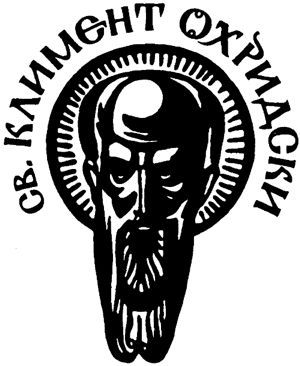
\includegraphics[width=0.1\linewidth]{su-logo.png}}
\chead{СОФИЙСКИ УНИВЕРСИТЕТ „Св. КЛИМЕНТ ОХРИДСКИ”\\Факултет по математика и информатика}
\fancyfoot[C]{\ifnum\thepage<2\relax\else\thepage\fi}
%end header definitions


%%custom commands
\tcbuselibrary{theorems}
\newtcbtheorem{definition}{Дефиниция}{colback=blue!5,colframe=blue!35!black,fonttitle=\bfseries}{def}
\makeatletter
\newcommand\tcb@cnt@definitionautorefname{Дефиниция}
\makeatletter

\newtcbtheorem{result}{Резултат}{colback=green!5,colframe=green!35!black,fonttitle=\bfseries}{res}
\makeatletter
\newcommand\tcb@cnt@resultautorefname{Резултат}
\makeatletter

%% Color definitions
\definecolor{darkgreen}{RGB}{1,127,1}
\definecolor{wine}{RGB}{128,0,1}
%% End Color Definitions

%%Autoref language settings begin
\renewcommand*{\figureautorefname}{Фиг.}
\renewcommand*{\equationautorefname}{Уравн.}
\renewcommand*{\subsectionautorefname}{Пар.}
\renewcommand*{\tableautorefname}{Табл.}
\renewcommand*{\subsubsectionautorefname}{\subsectionautorefname}
\newcommand{\subfigureautorefname}{\figureautorefname}
\renewcommand{\ALG@name}{Алгоритъм:}
\renewcommand{\fnum@algorithm}{\fname@algorithm}

%%Autoref language settings end


\makeatletter
\begin{document}
\begin{titlepage}
    \thispagestyle{fancy}
    \begin{center}
        \hfill \break
        \hfill \break
        \hfill \break
        \Huge	
        \textbf{Дипломна работа}\\
        \@title
        \vspace{3cm}
    \end{center}
    \normalsize	
    \title{}
    \vspace{2cm}

    \begin{flushright}
        \normalsize	
        От Може и без от!: \@author
        
        Магистърска програма: ,,Изчислителна математика и математическо моделиране``
        \vspace{1cm}

        Научен ръководител:

        \VT
    \end{flushright}

    \vspace*{\fill}
    \begin{center}
        \footnotesize	
        София, България\\
         ~\@date~
    \end{center}
 \end{titlepage}
\tableofcontents
\setcounter{page}{2}
\section{Въведение}
Целта на настоящата дипломна работа е да представи моделите и резултатите получени по време на работата ми през изминалата година с \vT. Крайната цел е да се моделира процеса на кристален растеж при различни условия и да се развие разбирането как експерименталните условия влияят на кинетиката на процеса и на крайната структура на кристала. В този контекст ще бъде направен и преглед на част от публикуваните експериментални данни с цел валидиране на моделите и подобряване на разбирането на тези резултати с разработените нови инструменти.

В най-общ смисъл настоящият труд може да бъде разделен на две основни части - моделиране на зависимостта на степента на превръщане $\alpha$ от времето (макроскопско моделиране) и моделиране на т.нар. ,,step-flow growth``  (моделиране на микроскопския механизъм). Преди това е нужно да бъде направено кратко въведение в представите за кристализацията като процес, разработени през късните години на миналия век.

\subsection{Критични явления и фазови преходи}
Кристализацията е от т.нар. ,,фазови преходи`` и по-точно е фазов преход от \textit{първи род}. Класификацията на фазови преходи от \textit{първи} и \textit{втори} род е дадена от Пол Еренфест \cite{Jaeger1998} \cite{atkinspaula2008} и представлява важен инструмент за разбирането на промените, които настъпват по време на процеса.

\begin{definition}{Класификация на Еренфест на фазовите преходи}{ehrenfest}
	По време на фазов преход от \textbf{n}-ти род, \textbf{n}-тата производна на вътрешната енергия ($\frac{\partial^n U}{\partial X^n}$) \textbf{U} по някоя термодинамична величина (\textbf{X}) търпи скок в критичната точка $\boldsymbol{X_c}$. \textbf{X} може да бъде температура (\textbf{T}), налягане (\textbf{p}), обем (\textbf{V}) и т.н.
\end{definition}

\noindent Физически важни са фазовите преходи от \textit{първи} и \textit{втори} род:

По време на фазов преход от \textit{първи род} съществуват едновременно и двете фази - течност/газ, течност/твърдо и т.н. Процеса е свързан и с т.нар. ,,латентна енергия``, което означава че системата приема или отдава фиксирано количество енергия (най-често топлина) за единица маса или обем. Системата тогава остава при постоянна температура по време на прехода като цялата отдадена/погълната енергия отива за формирането на новата фаза.

Фазовите преходи от \textit{втори род} се характеризират с плавна ($C^1$-непрекъсната) промяна на вътрешната енергия. Те обикновено са свързани със скок в т.нар. ,,възприемчивости`` на системата - магнитна възприемчивост, топлинен капацитет и други. Няма фазови граници между отделните фази и няма латентна топлина. Пример за такъв фазов преход е нагряването на магнит до неговата точка на Кюри. Характеристична за тези фазови преходи е безкрайната корелационна дължина в критичната точка. Прост модел за изследването на такива фазови преходи е моделът на Изинг за свойствата на феромагнитите в размерности на пространството по-големи от 1, който може да се приложи и за изследването на магнитните свойства на кристалите. Въпреки че тези фазови преходи са изключително интересни от физична и математическа гледна точка, те няма да бъдат предмет на настоящата работа.

\subsection{Термодинамика на кристализацията}
\label{sub:thermodynamics}
Имайки предвид \autoref{def:ehrenfest} естествен първи подход за моделиране на кристализацията е да използваме термодинамиката на многокомпонентните системи.

\begin{definition}{Химичен потенциал}{chempot}
    Химичният потенциал е промяната във вътрешната (свободната) енергия, която би настъпила при промяна на броя частици от даден химичен вид/фаза в системата. Най-често се отбелязва с $\mu$.
	\begin{equation}
		\label{eq:chempot}
		\mu_i = \left(\frac{\partial U}{\partial N_i}\right)_{S, V, N_{i \ne j}}
	\end{equation}
	Където индексът $S, V, N_{i \ne j}$ означава, че ентропията, обемът и броят други частици в системата са постоянни при изчисляване на производната.
\end{definition}

\noindent Следва да се отбележи, че абсолютната стойност на химичния потенциал не може да бъде измерена на практика. Нейната стойност (промяната ѝ) спрямо тази при определени референтни условия обаче може лесно да бъде получена експериментално. Затова и в литературата най-често се откриват табулирани стойностите на $\Delta \mu$ измерени по отношение на стандартни термодинамични условия ($T \approx 273~K, p \approx 1~atm$) \cite{IvanMarkovCGB}\cite{atkinspaula2008}.

\begin{result}{Условие за фазово/химично равновесие}{equil_cond}
	\[\sum\limits_i \nu_i\Delta \mu_i  = 0\]
	Където $\nu_i$ е т.нар. ,,стехиометричен коефициент``. За фазови преходи най-често $\nu_i = 1$ (една частица от фаза $\alpha$ преминава във фаза $\beta$).
\end{result}

\noindent Тогава можем директно да приложим уравнението за идеален разтвор към течната фаза:

\begin{align}
	\Delta \mu_{i} & = \left( \mu_{i}^\circ + RT\ln{c_i} \right) - \left( \mu_{i}^\circ + RT\ln{c_{i}^{eq}} \right) \nonumber \\
	\Delta \mu_{i} & = RT\ln{\frac{c_i}{c_{i}^{eq}}} \nonumber                                                                \\
	\Delta \mu_{i} & = RT\ln{\sigma} \label{eq:thermodynamic_force}                                                           
\end{align}

\noindent Където дефинираме:
\begin{equation}
	\label{eq:abs_supersat}
	\sigma \coloneqq \frac{c_{i}}{c_{i}^{eq}}
\end{equation}
Да бъде т.нар. ,,абсолютно пресищане``. Тогава \autoref{eq:thermodynamic_force}, заедно с условието за равновесие \autoref{res:equil_cond} ни дава термодинамичната движеща сила.

Кристализационният процес, от термодинамична гледна точка, е обусловен от абсолютното пресищане $\sigma > 1$. В граничния случай на равновесие $\sigma = 1$ ($c_{i}  = c_{i}^{eq}$). Този резултат е интуитивно смислен - ,,излишъкът``от частици в течната фаза преминават в кристалната \cite{IvanMarkovCGB}

Има много начини да бъде постигнато пресищане $\sigma > 1$ от експериментална гледна точка. Най-честият начин е наситен ($\sigma = 1$) за дадена температура разтвор да бъде охладен рязко, като други възможности са електрохимично да се промени разтворимостта, добавяне на друг електролит и разрушаване на солватната обвивка и т.н. 

Въпреки че термодинамичният модел е много лесен за получаване и разбиране, той единствено може да покаже коя е термодинамичната движеща сила, без да дава отговор на следните практически важни въпроси:
\begin{enumerate}
	\item Как започва кристалният растеж?
	\item Как скоростта на кристализация (трансформация) зависи от пресищането?
	\item Кристалите имат симетрия, която се репродуцира на всички мащаби. Какви са механизмите зад това?
	\item Как крайният размер на фазите влияе на растежа?
	\item \textbf{Какъв е микроскопският механизъм на процеса?}
\end{enumerate}

В следващите параграфи на това въведение ще бъде направен преглед на трудовете на Странски, Каишев, Кръстанов, Марков, Бъртон и др., който ще очертае основите на механизма възпроизводимият кристален растеж. Това ще послужи и като основа за моделите, които ще разработим.

\subsection{Микроскопски представи за кристалния растеж}
\label{sub:microscopic_growth}
Както беше споменато, горните разглеждания са чисто макроскопски и не взимат предвид реалното адсорбиране-десорбиране на градивните единици на кристалите - атоми, молекули, йони. Ще започнем прегледа като въведем някои общи дефиниции и нотация:
\begin{figure}[htbp]
	\centering
	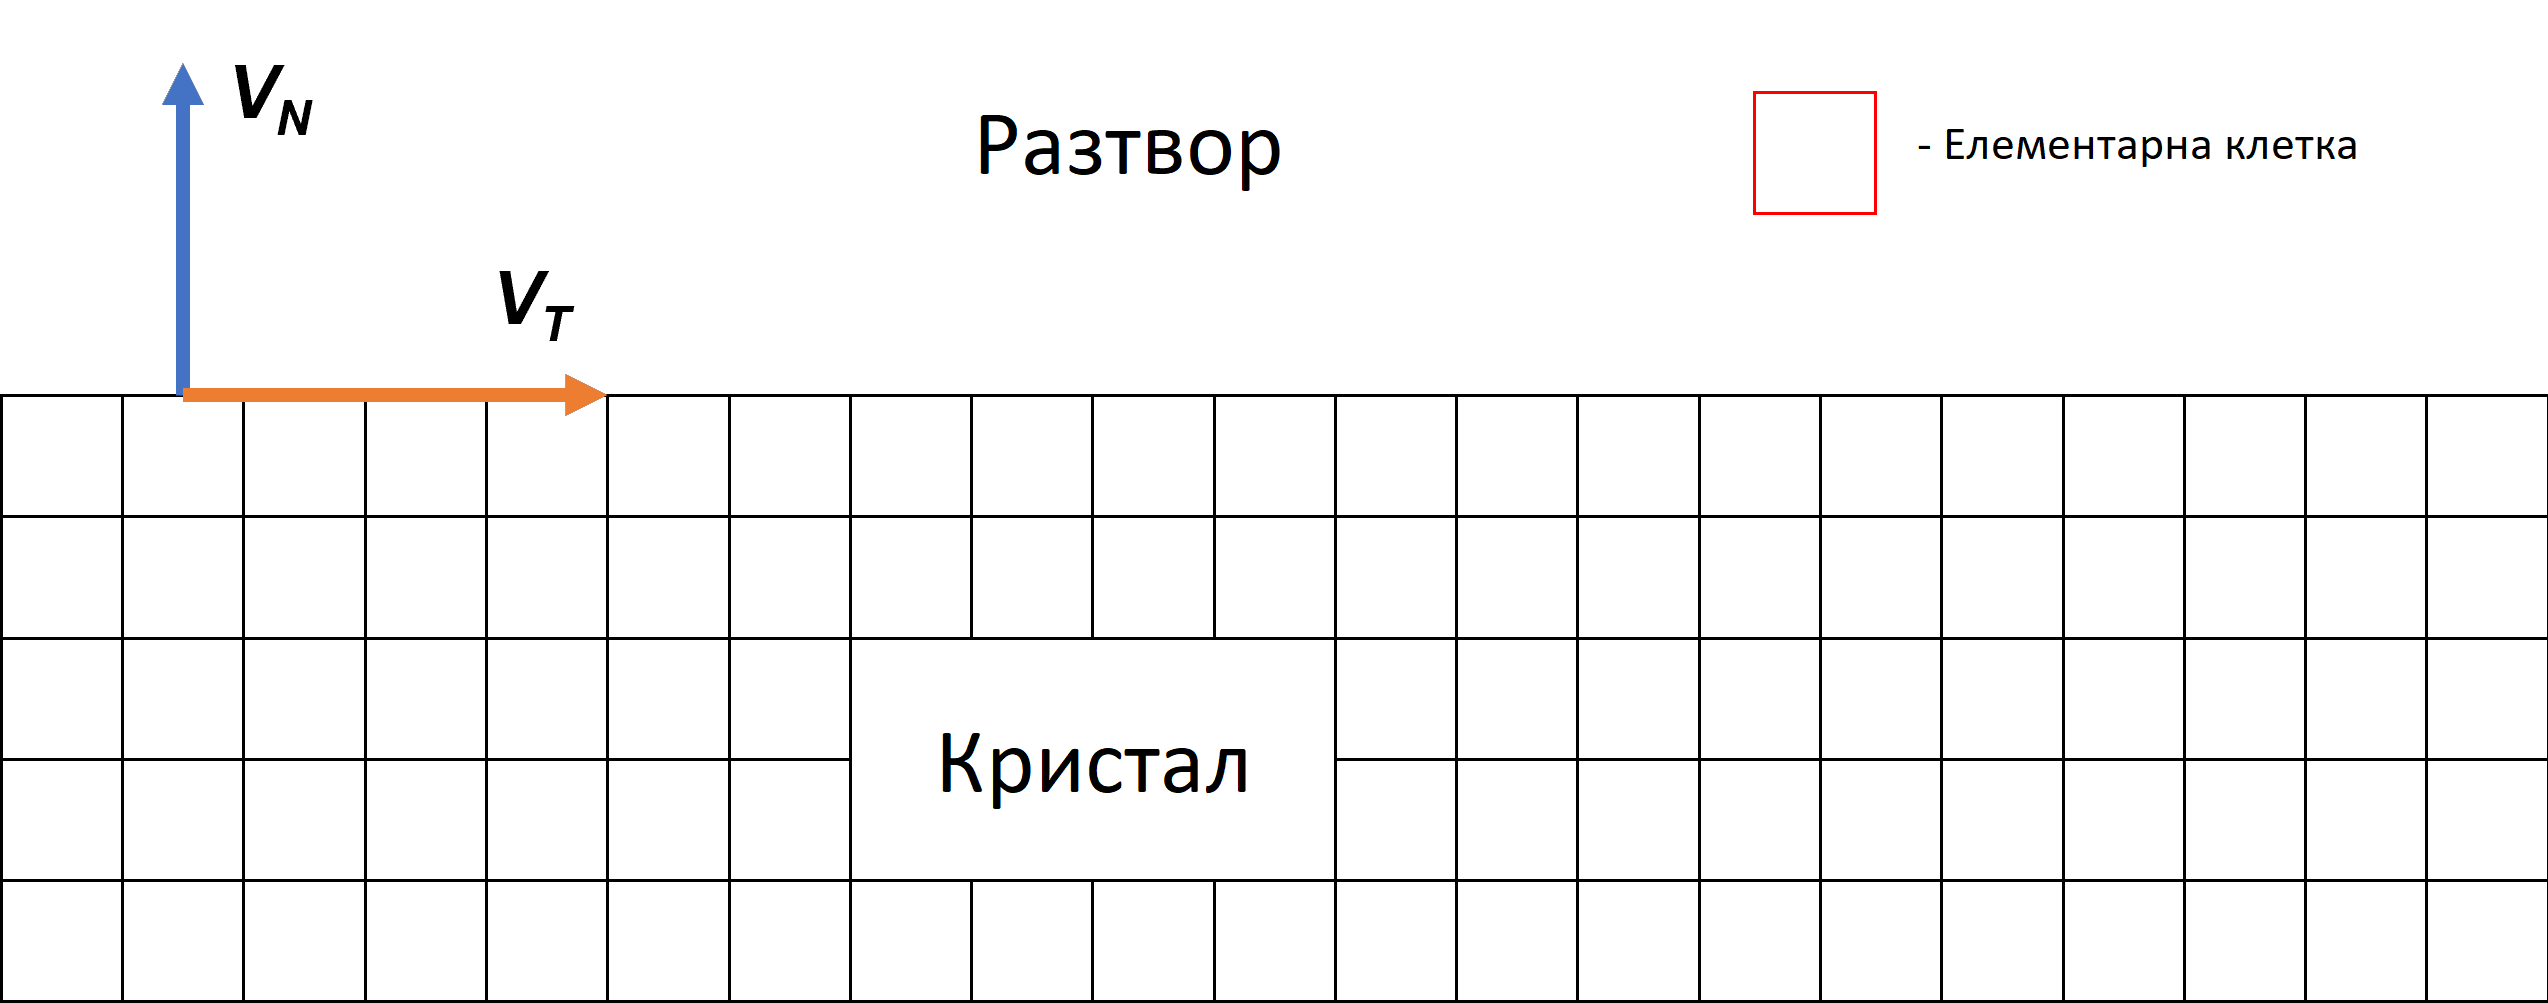
\includegraphics[width=\textwidth]{crystal_coord_system.png}
	\caption{Схематично представяне на растящ в разтвор кристал}
\end{figure}

\noindent Ще означаваме с $\boldsymbol{V_{N}}$ външната нормала към кристалната повърхност, а с $\boldsymbol{V_{T}}$ - единичния вектор тангенциален към повърхността. Също така ще предполагаме, че безкраен кристал без дефекти е изграден изцяло от т.нар. \textbf{елементарни клетки}, регулярно транслирани в посоките на пространството, така че да се получи плътна опаковка.

\begin{definition}{Елементарна клетка}{unit_cell}
    Елементарната клетка е най-малката структура от атоми, йони или молекули, която напълно отразява структурата на целия кристал. Целият кристал може да бъде изцяло изграден чрез транслиране на елементарната клетка по посока на главните координатни оси.
\end{definition}

Съществуването на повтаряща се структура като елементарната клетка, чиято група на симетрия се възпроизвежда на всички мащаби, дава една посоките за отговор на част от въпросите поставени в \autoref{sub:thermodynamics}. Кинетичният механизъм обаче остава все още неясен. За краткост като синоним на ,,елементарна клетка`` ще използваме понятието ,,градивна единица``.

\begin{figure}[ht]
	\centering
	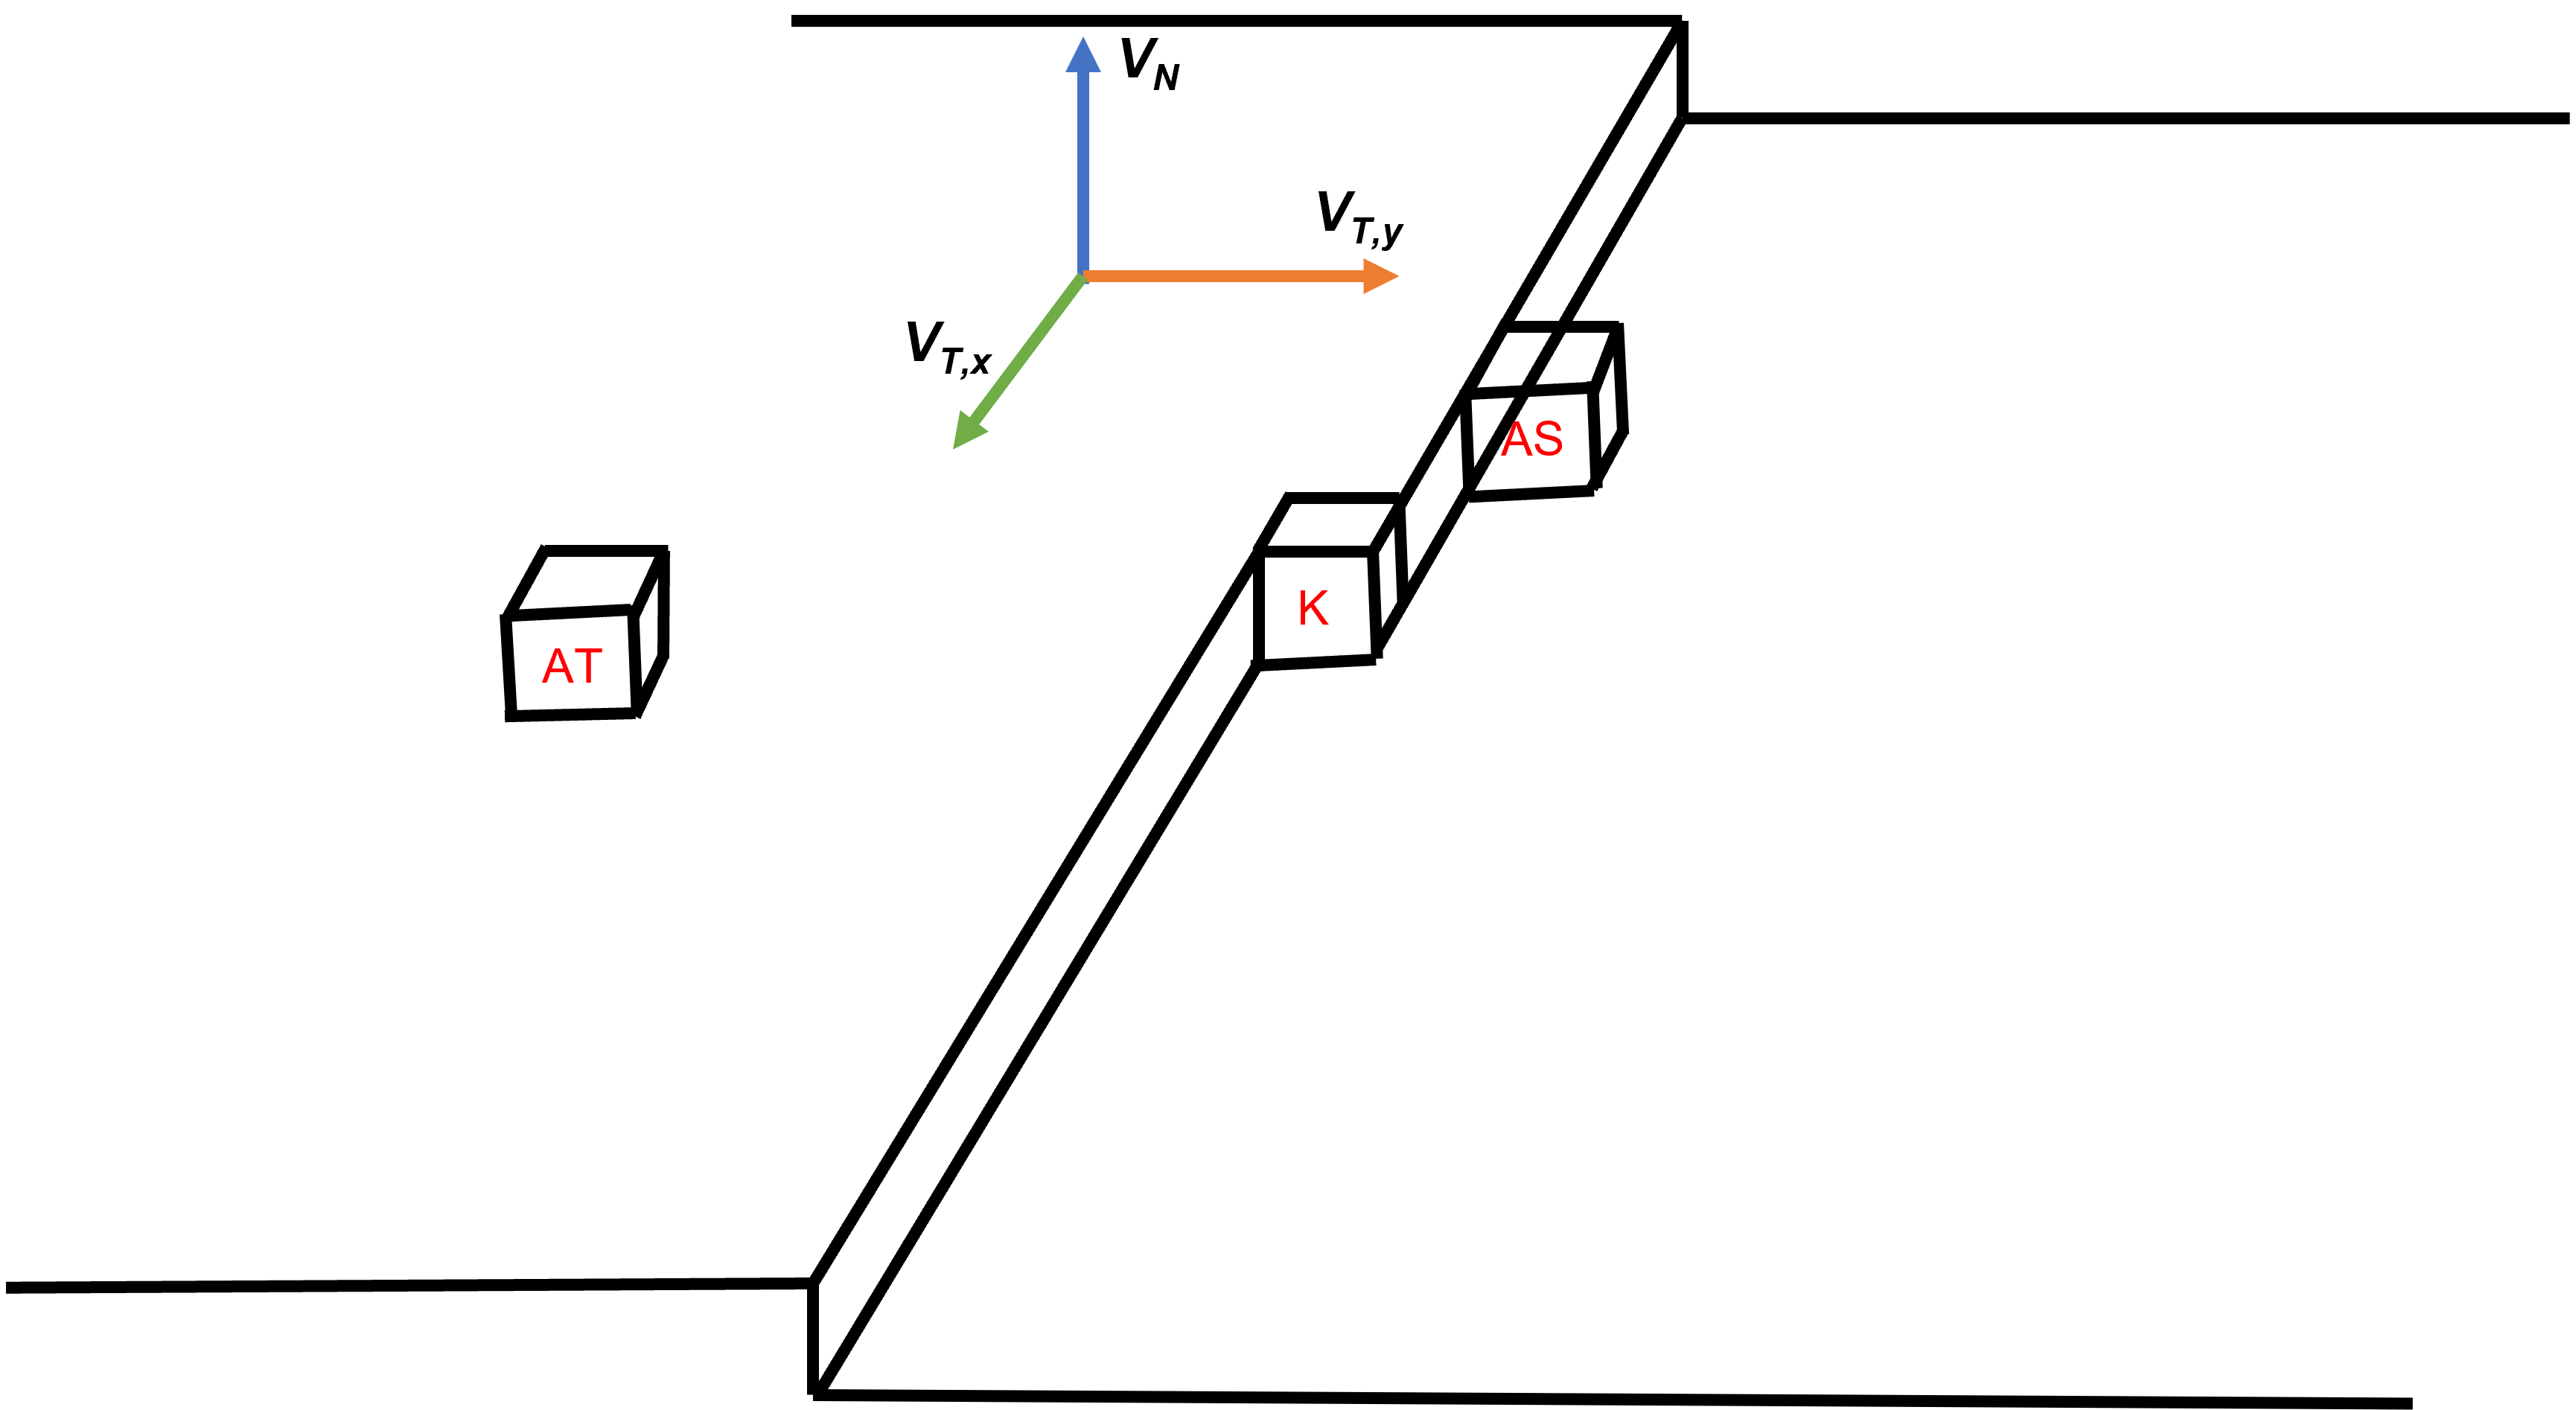
\includegraphics[width=\textwidth]{kink_pos.png}
	\caption{Позиции на растящата кристална повърхност:  \textcolor{red}{K} - кинк-позиция, \textcolor{red}{AT} - атом адсорбиран на терасата, \textcolor{red}{AS} - атом адсорбиран на стъпалото. }
	\label{fig:atoms_on_surface}
\end{figure}

Основите на съвременната кинетична теория поставят Странски и Косел независимо един от друг през 1927~г. \cite{Stranski1928}\cite{Kossel1927} като въвеждат идеята за работа, необходима за отделяне на градивна единица от т.нар. позиция на ,,полу-кристал`` или ,,кинк-позиция``. Тези представи свързват именно морфологията на растящата кристална повърхност с механизма на растеж.

От представените на  \autoref{fig:atoms_on_surface} позиции е ясно, че най-здраво свързани са атомите в обема на кристала. Новите адатоми обаче могат да се свържат само към повърхността му. В позиция \textcolor{red}{К} градивната частица има същият брой връзки като в обемния кристал, въпреки че са само ,,половин-връзки``, докато в позиции \textcolor{red}{AT} и \textcolor{red}{AS} e по-слабо свързана. Като следствие от това, свързването към кинк-позиция води до най-голямо понижаване на вътрешната енергия на свързващата се градивна единица и най-много отделена латентна топлина, и съответно е термодинамично най-устойчивата позиция. Това може да бъде илюстрирано още по-добре ако бъде разгледана и една странична (едномерна) проекция на растящата кристална повърхност, където представянето на кинк-позицията като най-енергийно изгодната такава става очевидно.

Такава проекция е представена на \autoref{fig:side_proj_kink}. От нея става освен това очевиден и друг централен факт - свързването към кинк-позиция води до формирането на нов кинк.
Това е основното ,,зъбно колело`` в механизма на възпроизводимия кристален растеж представен от Странски, Косел и Каишев \cite{Stranski1928} \cite{Kossel1927} \cite{StranskiKaischew1931}.
\begin{figure}[H]
	\centering
	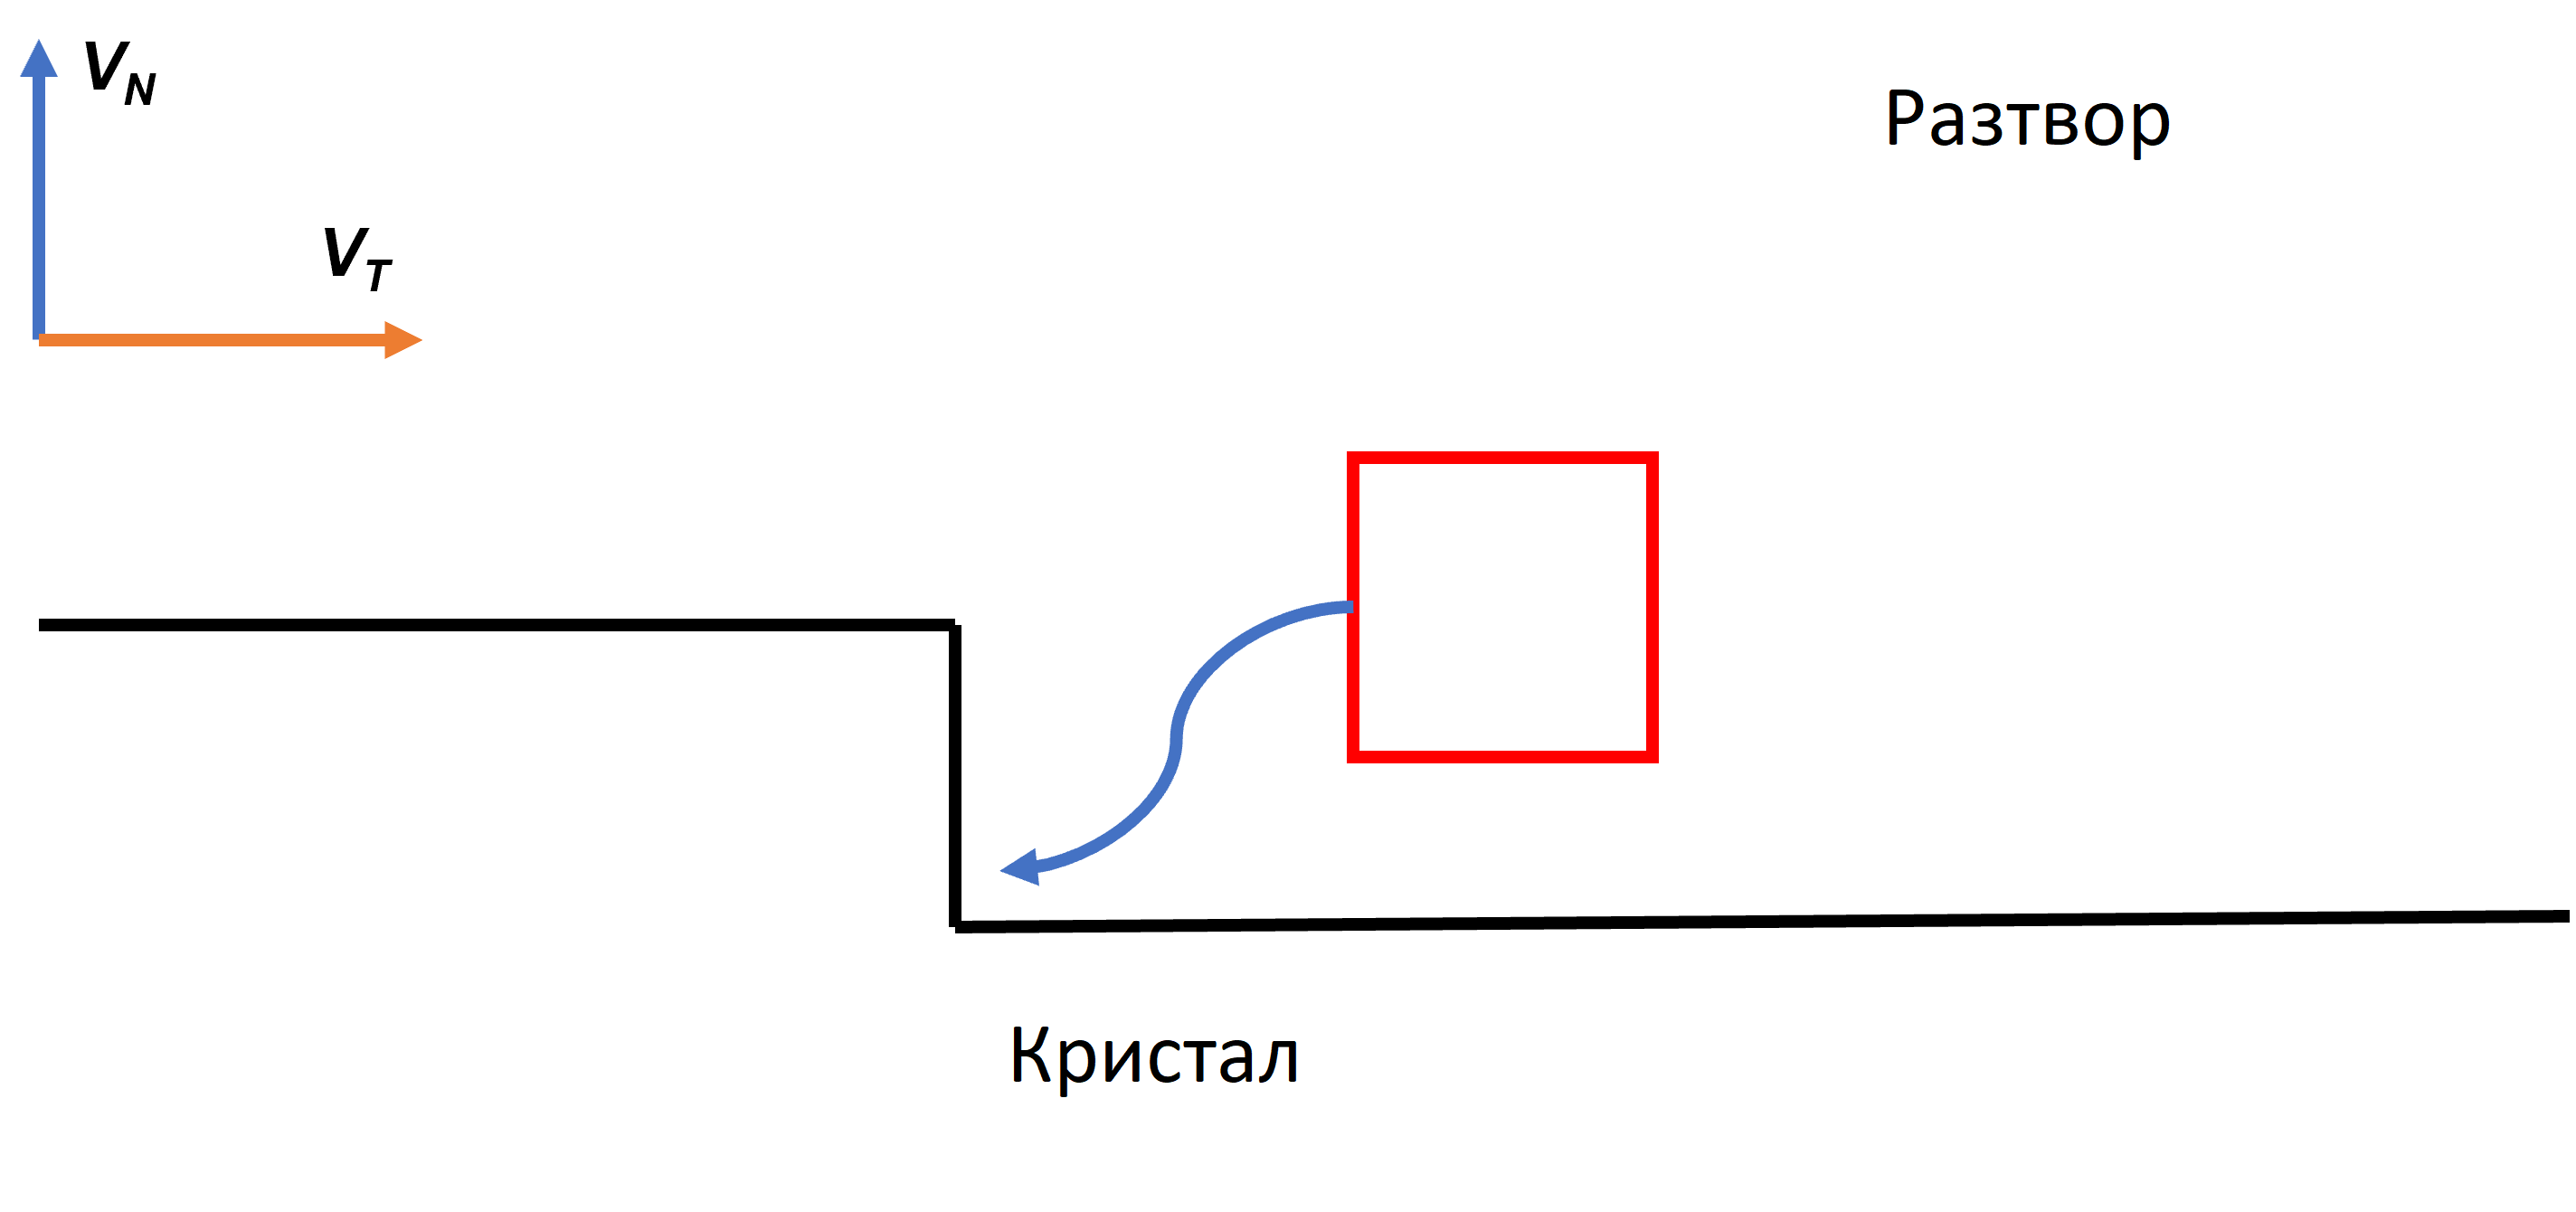
\includegraphics[width=\textwidth]{side_proj_kink.png}
	\caption{Странична (1D) проекция на кристалната повърхност}
	\label{fig:side_proj_kink}
\end{figure}

Идеята за кинк-позицията, комбинирана с тази за елементарната клетка като основна градивна единица, носеща цялата информация за кристала дава обяснение на въпроса за кристалната симетрия. Още повече, става ясно че растежът е послоен - новите градивни единици се свързват към кинк-позиции, докато настоящият слой от кристалната стена е изцяло изграден. Така ,,тангенциалният растеж`` (по посока на  $\boldsymbol{V_{T,x}}$ и $\boldsymbol{V_{T,y}}$) обуславя ,,нормалния`` (по посока на $\boldsymbol{V_{N}}$) и в крайна сметка - напредването на кристалната стена в разтвора.

От описаната картина обаче се вижда и недостатък на този механизъм - тъй като кристалите са крайни обекти, в даден момент всички кинкове са изчерпани. Затова към тези представи е необходимо да се добави и идеята за комплементарни събития на свързването към кинк-позиция. Природата на тези комплементарни събития може да е доста разнообразна - агрегация, зародишообразуване и т.н., но могат да бъдат обединени под общото название за ,,кинк-образуващи`` събития.
Процесът на образуване като правило може да е доста сложен - особено в случая на тримерен растеж, тъй като свързването на единствена градивна единица към атомно гладка кристална повърхност не води до образуване на кинк. Това ясно се вижда при позиция \textcolor{red}{AT} на \autoref{fig:atoms_on_surface}.

През 1931~г. Каишев и Странски доказват т.нар. теорема на \textit{Каишев-Странски-Волф} - градивни единици, които са свързани по-слабо от такава в кинк-позиция са ,,преходни`` - те не принадлежат към равновесната форма на кристала. Въпреки това, те могат да бъдат важна част от кинетиката на процеса (напр. като част от кинк-образуващи събития). \cite{StranskiKaischew1931}\cite{Yamamoto1988}

Комбинацията от тези идеи е довела до т.нар. ,,Terrace-Ledge-Kink`` (TLK) модел на кристалния растеж, който е бил предпоставка за основополагащия кинетичен модел на Бъртон-Кабрера-Франк (BCF), следствие от който ще бъде основа за нашите модели. \cite{BCF1951}\cite{Chernov2004}

През 30-те години на XX~век започва и паралелно развитие на модели за целите на металургията и описание на фазовите преходи, които могат да се наблюдават там. Ранните успехи на тази област до голяма степен се дължат на на Джонсън, Мел, Аврами и Колмогоров (JMAK) \cite{Mehl1939} \cite{Lambrigger1998}. Те успяват да изведат прост аналитичен модел за изследване на данни за т.нар. степен на превръщане $\alpha$ (интуитивно, какъв процент от кристализацията е приключила в даден момент от процеса).

\begin{result}{JMAKn}{jmak}
    Ще означаваме с JMAKn семейството от криви:
    \begin{equation}
        \label{eq:jmak}
        \alpha(t) = 1 - e^{ - k t^n }
    \end{equation}
    Където $\alpha$ - степен на превръщане, $n = D$ (D е броят на пространствените измерения, в които растежният процес се случва - 1, 2, 3) или $n = D+1$ (ако се наблюдава допълнително зародишообразуване), а $k$ - ,,материална константа`` (носеща температурната зависимост на процеса).
\end{result}

%% TODO: Maybe add graphs for different values of n in JMAKn

JMAKn е придобил широка популярност като основен инструмент за ,,фитване`` на данни със сигмодна форма от кристален растеж при разнообразни условия. Нещо повече - простотата на този модел го е направила толкова популярен, че до голяма степен условията и предположенията, при които е изведен са ,,забравени``. Могат да бъдат намерени публикувани експериментални данни, спрямо които е направена параметрична идентификация за $n$ в JMAKn и получените стойности не са целочислени (напр. $n = 1.725$) \cite{Min2005}. Това е довело до дискусии в областта дали кристалният растеж може да се случва в ,,брой`` пространствени измерения, който не е цяло число (т.нар. фрактален кристал), без първо да се вземе под внимание дали предпоставките, за които JMAKn е изведен са валидни за конкретните експериментални условия. Нецелите стойности на $n$ водят и до размерности на $k$, които трудно могат да бъдат обяснени (напр. какво би значело $[k]=T^{-1.725}$. Така възниква ситуация, в която се правят опити експериментът да бъде напаснат към и да обясни модела, а не обратното.

Съществуват и различни алтернативи на JMAKn, като най-често се използва моделът на Ричърдс - и по-точно неговите частни случаи - моделите на Гомперц и Ферхюлст. Тези сигмоидни криви при параметрични идентификация дават също малки остатъчни дисперсии, но пък са изведени за популационен растеж. Това прави също трудна физическата интерпретация на получените стойности.

Всички тези недостатъци на настоящите инструменти за моделиране на времевата еволюция на степента на превръщане $\alpha$ очертават нуждата за нов модел, изведен от първи принципи за изотермична кристализация от разтвор. Това ще бъде и целта на следващите параграфи.
\section{Моделът \texorpdfstring{$\aDg$}{αDg}} 
Преди да започнем с извеждането на модела, ще въведем малко обща нотация. Нека $\sigma_0$ бъде началното пресищане (за $t = 0 $) на разтвора (преди кристали да са се образували). Нека тогава $\sigma = \sigma(t)$ бъде пресищането в даден момент от време $t > 0$. Тогава дефинираме относителното пресищане като:
\begin{equation*}
	\Theta \coloneqq \frac{\sigma}{\sigma_0}
\end{equation*}
Така $\Theta \in [0,1]$ и е безразмерна величина, характеристична за моментното състояние на процеса.

Ще въведем и $r$  - магнитуда на нормалната скорост, с която кристалната стена напредва в разтвора. Съответно, $r_0$ ще е стойността на $r(t=0)$, която ще бъде важна скала при обезразмеряване на уравненията, които ще бъдат изведени по-долу.

Степента на превръщане $\alpha$, която беше / в контекста на JMAKn, сега ще дефинираме като:
\begin{equation}
	\label{eq:alpha_ndef_def}
	\alpha \coloneqq \frac{N(t)}{N_{max}}
\end{equation}

Където $N(t)$ е броят растящи кристали в момента $t$ и $N_{max}$ е максималният брой кристали, които ще се образуват при достигане на равновесие.

Ако предположим, че имаме $\eta$ кристала растящи едновременно, които не си взаимодействат през дифузионните си полета, тогава можем да дефинираме $\alpha$ през $D$-мерният обем на кристала. В такъв случай общото пресищане ще бъде разделено на броя растящи кристали поравно.

\begin{equation}
	\label{eq:alpha_vol_def}
	\alpha \coloneqq \frac{V(t)}{V_{max}}
\end{equation}

\noindent $\alpha \in [0,1]$ и също е безразмерна величина.

\subsection{Получаване на основното ОДУ на модела}
Стратегията за извеждане на основното ОДУ на модела ще бъде като започнем от следната форма на закона за запазване на масата:
\begin{equation}
	\label{eq:mass_conservation_law}
	\alpha(t) = 1 - \Theta(t)
\end{equation}
\noindent Физическият смисъл на \autoref{eq:mass_conservation_law} е следният: една частица може да е или в разтвора и да допринася за относителното пресищане или да е в кристала и да допринася за степента на превръщане.

Нататък продължаваме с основното следствие от BCF-модела \cite{BCF1951} и го комбинираме с \autoref{eq:mass_conservation_law}:
\begin{equation}
	\label{eq:bcf_corollary}
	r = r_0(g)(1-\alpha)^g
\end{equation}

\noindent Където $g$ е параметър от BCF модела. Каноничните стойности за $g$ са \textit{1} в режима на бърза кинетика (дифузионно контролиран растеж) и \textit{2} за кинетично контролиран.

\autoref{eq:bcf_corollary} записано в този вид напомня на закона за действие на масите (ЗДМ) на  \textit{Гулдберг и Вааге} и по тази причина параметърът $g$ понякога се нарича \textit{порядък на растеж}. Тук следва да се отбележи, че трябва тази аналогия със ЗДМ да се ползва внимателно, тъй като в лявата страна на уравнението $r$ е скоростта на фронта, а не производна на концентрацията (скорост на химична реакция - chemical rate). Още повече, това движение на кристалната стена е ефективно - всяка свързала се единица остава фиксирана към нея.

\noindent Общата скорост на растеж се дефинира като:
\begin{equation}
	\label{eq:overall_growth_rate}
	G \coloneqq \frac{dl}{dt}
\end{equation}
Където $l$ - линеен характеристичен размер на кристала (напр. полудължина на нишката при едномерен растеж, страна на квадрат при двумерен, страна на куб при тримерен).
При т.нар. \textit{полиедричен} растеж всеки две срещуположни стени нарастват едновременно спрямо центъра (началния зародиш). Т.е. общата скорост на растеж е два пъти скоростта на напредване на стената: $G = 2r$, за да се запази полиедричната форма на кристала.
В експерименти, при които пресищането се довежда до своята максимална стойност в началото и след това не се поддържа допълнително, както и допълнителното зародишообразуване е потиснато (напр. двойно-импулсната техника) фиксиран малък брой кристали $\eta$ растат и имат един и същ характеристичен размер $l$. Това ни позволява да разглеждаме случая, когато кристалите не си взаимодействат с дифузионните си полета. Допълнително, в такива условия е по-вероятно дифузията да е бавна и съответно $g = 1$.

Растежът приключва когато кристалите достигнат своята максимална характеристична дължина $l_{max}$. Може да се покаже чрез анализ на размерностите за $l_{max}$ \cite{Tsoularis2002}:
\begin{equation}
	\label{eq:l_max}
	l_{max} = f\left(N^{-\frac{1}{D}}, (c-c_{eq}) \right)
\end{equation}
Ще обезразмерим \autoref{eq:overall_growth_rate} като използваме $l_{max}$ като естествената скала за дължина:
\begin{equation}
	\label{eq:half_non_dimensional}
	l_{max} \frac{d(l/{l_{max}})}{dt} = 2r_0(g)(1-\alpha)^g
\end{equation}
Тогава получаваме времевата скала на процеса $\tau$ по естествен начин.
\begin{equation}
	\label{eq:time_scale}
	\tau \coloneqq \frac{l_{max}}{r_0(g)}
\end{equation}
Заедно с \autoref{eq:l_max}, получаваме че $\tau \propto N^{-(1/D)}$. Можем да сравним с известната от литературата скала на JMAKn \cite{Avramov2005}:
\begin{equation}
	\label{eq:jmak_time_scale}
	\tau_{JMAKn} \propto \frac{1}{U N^{1/D}}
\end{equation}
Където $U$ e постоянната скорост на повърхностите. Това съответствие в скалите ще стане още по-важно по-късно при по-детайлно сравнение на $\aDg$ моделите с JMAKn. Тогава ще покажем, че $\tau \approx 1.1 \tau_{JMAKn}$ в общия случай.

\noindent Връщайки се към \autoref{eq:half_non_dimensional} можем да го запишем в изцяло безразмерна форма:
\begin{equation}
	\frac{d(l/l_{max})}{d(t/\tau)} = 2(1-\alpha)^g
\end{equation}
Според \autoref{eq:alpha_vol_def} можем да разглеждаме степента на превръщане $\alpha$ като рескалирания обем на кристала(ите). Тогава при $D$-мерен растеж имаме:
\begin{equation*}
	l/l_{max} = \alpha^{1/D}
\end{equation*}
Заместваме горното и диференцираме:
\begin{align*}
	\frac{d \alpha ^ {1/D}}{d(t/\tau)}            & = 2(1-\alpha)^g \\
	\frac{\alpha^{(1-D)/D} d \alpha}{D d(t/\tau)} & = 2(1-\alpha)^g 
\end{align*}
Така довършвайки преобразованието и замествайки $\alpha \rightarrow \aDg$, за да отбележим конкретна крива при даден избор на $D, g$ получаваме:
\begin{result}{Основно ОДУ на $\aDg$ моделите}{adg_main_ode}
	\begin{equation}
		\label{eq:main_aDg_ode}
		\frac{d\aDg}{d(t/\tau)} = 2D\aDg^{(D-1)/D}(1-\aDg)^g
	\end{equation}
	Естественото начално условие, с което да затворим диференциалната задача е $\aDg(0) = 0$ - в началото няма формирани кристали.  
\end{result}
\noindent \autoref{eq:main_aDg_ode} с това начално условие ще бъде основното диференциално уравнение, което ще изследваме в тази част.

\subsection{Анализ на основното ОДУ}
От самото ОДУ - \autoref{eq:main_aDg_ode} се вижда, че имаме два противостоящи си механизма - такъв на положителна (,,автокаталитичен``) и на отрицателната (,,самоограничаващ``) обратна връзка. 

Положителната обратна връзка се определя от $2D\aDg^{(D-1)/D}$ члена и е независима от стойността на g. Освен това се вижда директно за $D = 1$, че този член е константата $2$ и съответно такава обратна връзка няма в процеса. При $D = 2$ положителната обратна връзка е $4\alpha_{2g}^{1/2} = 4 (l/l_{max})$ - рескалираният периметър на двумерния кристал, т.е. с нарастването на периметъра този член води до ускоряване на процеса. При $D = 3$ имаме  $6\alpha_{3g}^{2/3} = 6 (l/l_{max})^2$ - околната повърхнина на растящия куб. От основното ОДУ имаме, че положителната обратна връзка е доминираща за ,,малки`` $\alpha$, т.е. $\alpha \rightarrow 0$. Тогава можем да разгледаме дясната страна на уравнението в тази граница. 
\begin{equation}
	\label{eq:main_aDg_ode_small_limit}
	\frac{d\aDg}{d(t/\tau)} = 2D\aDg^{(D-1)/D}
\end{equation}
Това уравнение може да бъде интегрирано лесно:
\begin{equation}
	\label{eq:aDg_small_alpha_limt}
	\alpha(t) = \left(\frac{2t}{\tau}\right)^D
\end{equation}
От \autoref{eq:main_aDg_ode_small_limit} и \autoref{eq:aDg_small_alpha_limt} наблюдаваме следните важни следствия:

Положителната обратна връзка, освен че доминира при $\alpha \rightarrow 0$, тя е от вида $\aDg \propto t^D$. Т.е. в началото имаме ,,бърз`` полиномиален растеж, като поради участието на повече стени в околната повърхнина при по-големи D, имаме по-бърз начален растеж.
\autoref{eq:main_aDg_ode} също така много напомня за диференциалната форма на класическия модел на Ферхюлст. Тук нарочно ще отбележим функцията за която е записано ОДУ на модела с $\alpha$ и ще изберем за скоростта на растеж $k = 2D$, с цел да подчертаем аналогията 
\begin{equation}
	\frac{d\alpha}{d(t/\tau)} = 2D\alpha (1-\alpha)
\end{equation}
Тук освен че отрицателната обратна връзка съвпада със случая $g = 1$, струва си да се фокусираме върху положителната:
\begin{equation*}
	\frac{d\alpha}{d(t/\tau)} = 2D \alpha
\end{equation*}
Интегрираме и получаваме за същото начално условие:
\begin{equation*}
	\alpha(t) = e^{2Dt} - 1
\end{equation*}

От тези разгледания можем директно да заключим, че при направените предположения растежът в началото винаги ще е по-бавен от такъв отговарящ на модела на Ферхюлст. Това се потвърждава и от факта, че степента на положителната обратна връзка в \autoref{eq:main_aDg_ode} е $1-\frac{1}{D}$, т.е. с нарастването на пространствените измерения се доближаваме до растеж по Ферхюлст, като за $D \rightarrow \infty$ съвпадението е точно. Не бива да забравяме, че $D > 3$ в рамките на този модел не са физически смислени стойности.

Отрицателната обратна връзка води до самоограничаване (регулиране) на растежния процес, т.е. с изчерпването на пресищането процеса започва да се забавя. Тоест този член започва да доминира в случаите когато $\aDg \rightarrow 1$. Изолирайки само тази част от ОДУ получаваме:
\begin{equation}
	\frac{d\alpha}{d(t/\tau)} = (1-\alpha)^g
\end{equation}
Тук трябва да сме внимателни при интегрирането, като за $g=1$ получаваме:
\begin{equation*}
	\alpha(t) = 1-e^{-t/{\tau}}
\end{equation*}
За $g = 2$:
\begin{equation*}
	\alpha(t) = 1 - \frac{\tau}{t}
\end{equation*}
И в двата случая получаваме монотонно растящи към $1$ при $t \rightarrow \infty$ функции. Така виждаме, че когато пресищането започне да се изчерпва, отрицателната обратна връзка ограничава растежа, $\alpha$ да бъде най-много $1$ (целият излишък е в твърдата фаза).

\begin{figure}[ht]
	\centering
	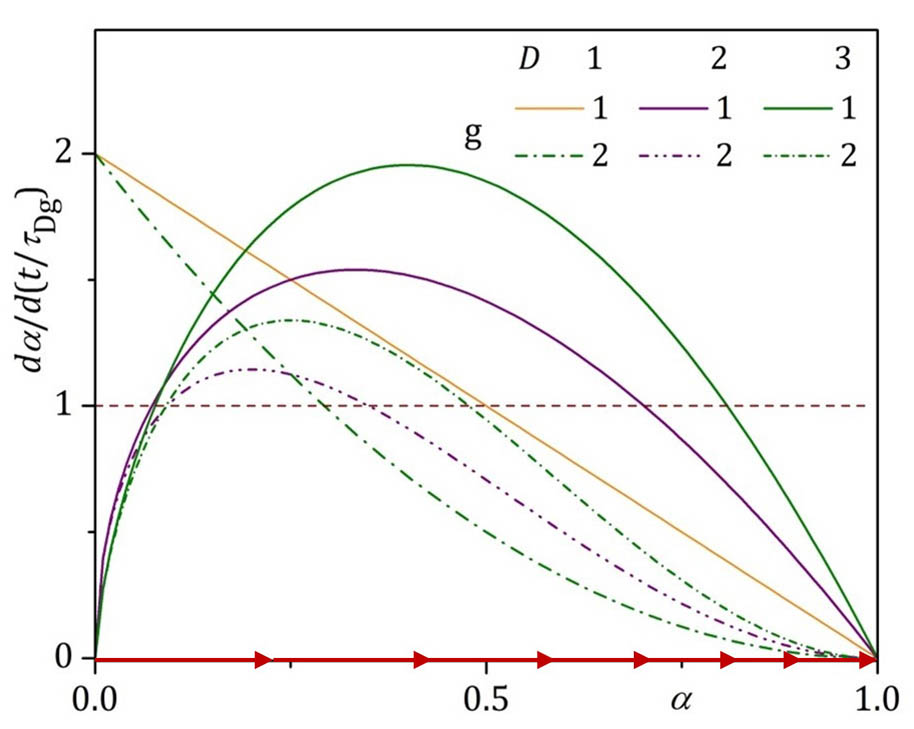
\includegraphics[width=0.9\textwidth]{phase_space.jpg}
	\caption{1D фазово пространство (линия) на модела. Представени са физически важните стойности на параметрите $D$ и $g$.}
	\label{fig:aDg_phase_space}
\end{figure}

Друг важен инструмент за разбирането на поведението на моделите при различен избор на параметрите е фазовата линия (едномерното фазово пространство) представена на фигура \autoref{fig:aDg_phase_space}. От него първото важно наблюдение е, че независимо от избора на параметри $\aDg  = 0 $ и $\aDg = 1$ са двете равновесни точки на системата. Нещо повече - единствената глобално асимптотично устойчива равновесна точка е $\aDg = 1$, докато $\aDg = 0$ е неустойчива. 

Това има последствия за интегрирането - числено и аналитично. Началното условие $\aDg (0) = 0$ се изпълнява и от тривиалното решение $\aDg(t) = 0$, $\forall t > 0$. Този проблем лесно може бъде съобразен и избегнат при аналитичното интегриране на ОДУ. При численото интегриране, което ще правим, за да сме сигурни че ще получим ,,интересното`` решение ще избираме $\aDg = \epsilon$, където $\epsilon > 0$ e ,,малко`` число, близко до машинната грешка (но по-голямо от нея). Тъй като  $\aDg = 1$ е устойчива равновесна точка, грешката от това числено решение ще бъде малка спрямо точното и бихме очаквали да намалява с нарастване на времето (при условие, че численият метод за интегриране има ,,добро`` поведение.

От \autoref{fig:aDg_phase_space} се оправдава и очакването ни за сигмоидния ход на кривите, преди да сме получили решения за ОДУ. Всички модели (без $D=1$) имат инфлексна точка, в която доминиращата обратна връзка се сменя от положителна на отрицателна. Добре се очертава и монотонното намаляване на скоростта при моделите, в които няма положителна обратна връзка ($D=1$). При тях максималната скорост на растеж е била началната, след което процесът само се забавя до ,,достигане`` на равновесие.

\subsection{Получаване на аналитични изрази}
\label{sub:analytic_results}
Разделяме променливите в \autoref{eq:main_aDg_ode} и интегрираме. За простота на записа правим смяната $t \rightarrow t/\tau$. Така получаваме следната имплицитна крива:
\begin{equation}
	\label{eq:integral_aDg_beta_implicit}
	t(\alpha) = \frac{1}{2D}\mathcal{B}\left(\alpha; \frac{1}{D}, 1 - g \right)
\end{equation}
Където $\mathcal{B}\left(x; a, b \right) = \int_{0}^{x} t^{a-1} (1-t)^{b-1} dt$ е непълната не-нормирана бета-функция на Ойлер. Използвайки нейната обратна, можем да запишем формално:
\begin{equation}
	\label{eq:integral_aDg_beta_inverse}
	\alpha(t) = \mathcal{B}^{-1}\left( 2Dt; \frac{1}{D}, 1 - g \right)
\end{equation}
Където съответно $\mathcal{B}^{-1}$ е обратната на бета-функцията. 

Това решение е достатъчно общо, но получаване на затворени изрази за произволни стойности на параметрите $D, g$ в общия случай не е възможно. За целта е разработена и числена процедура, която да интегрира основното ОДУ за произволен избор на параметрите.

Въпреки това, за физически обоснованите, целочислени стойности на параметрите, т.е. $D = 1, 2, 3$ и $g = 1, 2$ е възможно да извършим аналитично интегрирането. За случаите $D + g \le 3$ можем да получим изрази в затворен вид, докато за $D + g > 3$ можем да получим само кривите $t(\alpha)$. Резултатите от интегрирането обобщаваме така:
\begin{align*}
	\noindent\text{За $g = 1:$} \\
	    & \alpha_{11} =  1 - \exp{\left(-2t/\tau_{11}\right)}                                                                                                                                                                                                                                                             \\
	​ & \alpha_{21} = \tanh^2 \left(2 t/\tau_{21}\right)                                                                                                                                                                                                                                                                 \\
	    & \frac{t}{\tau _{31}} = \frac{1}{12} \left(\ln \left(\frac{\alpha_{31}^{2/3}+\sqrt[3]{\alpha_{31}}+1}{\left(1-\sqrt[3]{\alpha_{31}}\right){}^2}\right)+2 \sqrt{3}\arctan\left(\frac{\sqrt{3} \sqrt[3]{\alpha_{31}}}{2+\sqrt[3]{\alpha _{31}}}\right)\right) \tag{*}                                               \\
	\noindent\text{За $g = 2:$} \\
	    & \alpha_{12} = \frac{2 t/ t_{12}}{2 t/ t_{12} + 1}                                                                                                                                                                                                                                                                \\
	    & t/\tau_{22} = \frac{1}{4}\left( \frac{\alpha_{22}^{1/2}}{1-\alpha_{22}} + \tanh^{-1} \alpha_{22}^{1/2} \right) \tag{*}                                                                                                                                                                                           \\
	    & \frac{t}{\tau_{32}} = \frac{1}{18} \left(\frac{3 \sqrt[3]{\alpha_{32}}}{1-\alpha_{32}}+\ln \left(\frac{\alpha_{32}^{2/3}+\sqrt[3]{\alpha _{32}}+1}{\left(1-\sqrt[3]{\alpha_{32}}\right){}^2}\right)+2 \sqrt{3}\arctan \left(\frac{\sqrt{3} \sqrt[3]{\alpha_{32}}}{2+\sqrt[3]{\alpha_{32}}}\right)\right) \tag{*} 
\end{align*}
Уравненията, които са отбелязани с $(*)$ не могат да бъдат решени за $\aDg$.
\begin{figure}[H]
	\centering
	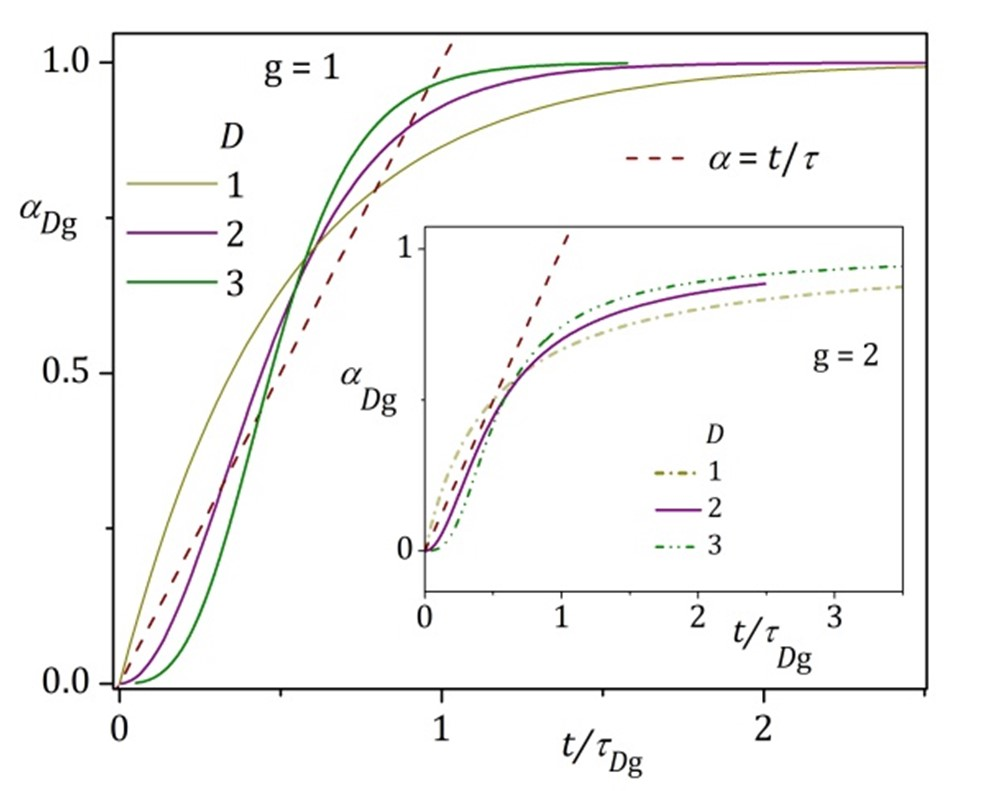
\includegraphics[width=0.9\textwidth]{integral_curves.jpg}
	\caption{Интегрални криви на модела. Основна фигура: $g = 1$, вложена: $g = 2$. Тук правата отговаряща на $\alpha = t/\tau$ е дадена като референтна за по-удобно сравняване на двете фигури.}
	\label{fig:aDg_integral_curves}
\end{figure}

\subsection{Инфлексни точки на модела}
\label{sub:aDg_infl_points}
Както вече беше споменато, в модела имаме два вида обратна връзка - положителна и отрицателна. Точката, в която доминиращата обратна връзка се сменя, е инфлексната точка (когато тя съществува). В този смисъл инфлексната точка е характеристична за режима на кристален растеж, който наблюдаваме и затова получаването на израз за нея като функция на параметрите на модела ще бъде важна задача, която да решим. Необходимо условие за съществуването на инфлексна точка $t^*$ е:
\begin{equation*}
	\alpha'' = \left. \frac{d^2\alpha}{dt^2}\right|_{t = t^*} = 0
\end{equation*}
Диференцираме двете страни на \autoref{eq:main_aDg_ode} по t:
\begin{equation*}
	\alpha'' = -2 \alpha^{-1/D} (1-a)^{g-1}\left[ \left( D g + D - 1 \right)\alpha - D + 1 \right] \alpha'
\end{equation*}
Заместваме $\alpha'$ с дясната страна на \autoref{eq:main_aDg_ode}, групираме членовете по $\alpha$ и получаваме за втората производна:
\begin{equation}
	\label{eq:aDg_second_der}
	\alpha'' = -4 D \alpha^{\frac{D-2}{D}}(1-\alpha)^{2g-1}\left[(D g + D - 1) \alpha - D + 1\right]
\end{equation}
Единствената нула $\alpha^*$ на уравнението $\alpha'' = 0$, която не е една от равновесните точките $\alpha = 0 $ или $\alpha = 1$ e:
\begin{equation}
	\label{eq:aDg_alpha_infl_point}
	\alpha^* = \frac{D - 1}{D g + D - 1}, \qquad D > 1
\end{equation}  
Тъй като в $\alpha_{1g}$ моделите няма положителна обратна връзка, те нямат и инфлексна точка. Това се потвърждава и от монотонно намаляващите криви на \autoref{fig:aDg_phase_space}.
Тук общото решение дадено в \autoref{eq:integral_aDg_beta_implicit} за $t(\alpha)$ ще ни послужи да намерим за кое $t^*$ се достига инфлексната точка $\alpha^*$ (изчисляването на правата непълна ненормирана бета-функция е много по-лесна и добре обусловена числена задача от тази за обратната). Можем да обобщим като кажем, че $\aDg$ моделите имат инфлексна точка в наредените двойки $\{t^*, \alpha^*\}$, такива че:
\begin{equation}
	\label{eq:aDg_tuple_infl_point}
	\left\{t^*; \alpha^* \right\} = \left\{\frac{1}{2D}\mathcal{B}\left( \frac{D - 1}{D g + D - 1}; \frac{1}{D}, 1 - g \right); \frac{D - 1}{D g + D - 1}\right\} 
\end{equation}
Конкретните стойности можем да обобщим в \autoref{tabl:aDg_infl_points}. Интересно наблюдение е, че инфлексните точки са относително ,,рано``, т.е. за ,,малки`` $t, \alpha$, и по-конкретно $\alpha^* < 1/2$ за всеки от наборите параметри. Това е логично, предвид че положителната обратна връзка е ,,по-слаба`` от експоненциалната в модела на Ферхюлст, т.е. процесът на кристален растеж при тези условия се самоограничава относително бързо и  съответно максимумът на скоростта се достига относително рано. Още по-явно се забелязва това в случая на кинетичен контрол, когато $g = 2$. Тогава самоограничаването на процеса е още по-силно.

Интересен факт е, че инфлексните точки са относително ,,близо`` до правата $\alpha = t/\tau$, т.е. използването ѝ като референтна такава на \autoref{fig:aDg_integral_curves} е оправдано за целите на сравняване на хода на кривите.
\begin{table}[htbp]
	\centering
	\caption{Инфлексни точки на $\aDg$ моделите при различни стойности на параметрите $D, g$}
	\label{tabl:aDg_infl_points}
	\resizebox{0.5\textwidth}{!}{%
		\begin{tabular}{@{}cll@{}}
			\toprule
			\multicolumn{1}{l}{D/g} & \multicolumn{1}{c}{1} & \multicolumn{1}{c}{2} \\ \midrule
			1                       & -                     & -                     \\
			2                       & \{0.329; 1/3\}        & \{0.260; 1/5\}        \\
			3                       & \{0.417; 2/5\}        & \{0.365 ; 1/4\}       \\ \bottomrule
		\end{tabular}%
	}
\end{table}
\subsection{Числено интегриране и параметрична идентификация}
\subsubsection{Числено интегриране}
\label{subsub:numeric_integration}
Както беше споменато в \autoref{sub:analytic_results} аналитичното интегриране е трудно за произволни параметри $D, g$. Същевременно ,,обръщането`` на бета-функцията е лошо обусловена числено задача. Причината за това е, че при $\alpha \rightarrow 1$, $t \rightarrow \infty$, т.е. за големи степени на превръщане числените методи за решаване на \autoref{eq:integral_aDg_beta_implicit} ще стават неустойчиви, тъй като задачата е лошо обусловена, независимо от конкретните качества на метода.

От друга страна знаем от \autoref{fig:aDg_phase_space}, че равновесната точка $\alpha = 1$ e устойчива \autoref{eq:main_aDg_ode}. Нещо повече, чрез директно прилагане на правилото за Лайбниц за $n$-та производна на произведение, получаваме че $f^{(n)} (\alpha = 1)  = 0$. Където с $f(\alpha) = 0$ сме означили дясната страна на \autoref{eq:main_aDg_ode}. Т.е. не очакваме да имаме проблеми с устойчивостта на методите.

Директно можем да се възползваме от библиотеката \textit{Scipy} \cite{2020SciPy-NMeth} за програмния език \textit{Python}. \textit{Python} е особено подходящ заради динамичната си типова система, която позволява на функцията \textit{scipy.integrate.solve_ivp()} директно да върне кубичен ермитов сплайн-интерполант на решението в интервала $[t_0, t_{max}]$. 
Единствената особеност тук е, че за да сме сигурни че няма да останем в тривиалното решение $\aDg(t) = 0, \forall t$, ще вземем за начално условие $\aDg(0) = 10^{-10}$.
\begin{minted}{python}
def get_sigmoid(d, g):
    sol = integrate.solve_ivp( # from scipy
        rhs, # 2 * d * ((1 - y) ** g) * (y ** (1 - (1 / d)))
        [SIGMOID_CONFIG["t0"], SIGMOID_CONFIG["t_final"]],
        [SIGMOID_CONFIG["initial_alpha"]],
        args=(d, g),
        dense_output=True,
        method="RK45",
        atol=1e-13,
        rtol=1e-12
    )
    return sol.sol # returns a function object
\end{minted}
Полученият обект е изключително удобен за последваща работа, защото има поведение на функция на един аргумент, която за дадено $t/\tau$ връща стойността на $\alpha$. Конкретната имплементация, която е с по-общ програмен интерфейс може да бъде намерена в скрипта \textit{sigmoid_calculation.py} от \cite{SigmoidToolsGH}.

Резултатите от численото интегриране на $\alpha_{21}$ са показателни за общото поведение на числената процедура и за други избори на параметрите на модела.
\begin{figure}[!ht]
    \centering
    \caption{Числено интегриране до различни $t/\tau$}
        \subfloat[Малки времена]{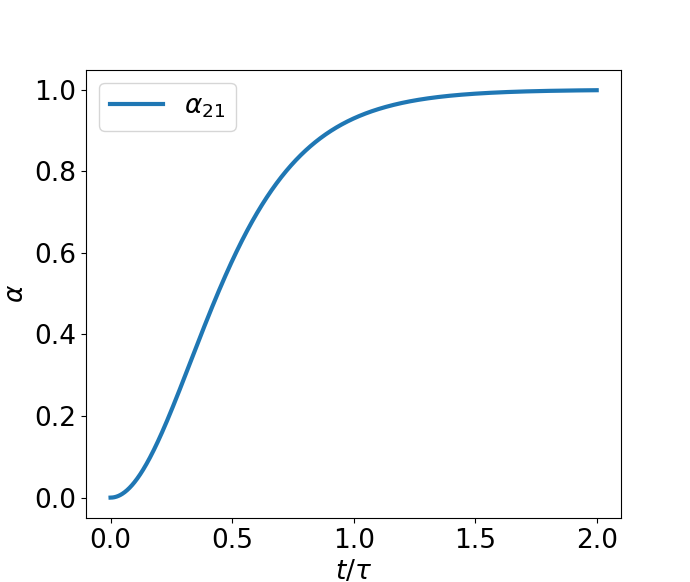
\includegraphics[width=0.47\textwidth]{alpha21_small_tmax.png}}
        \subfloat[Големи времена]{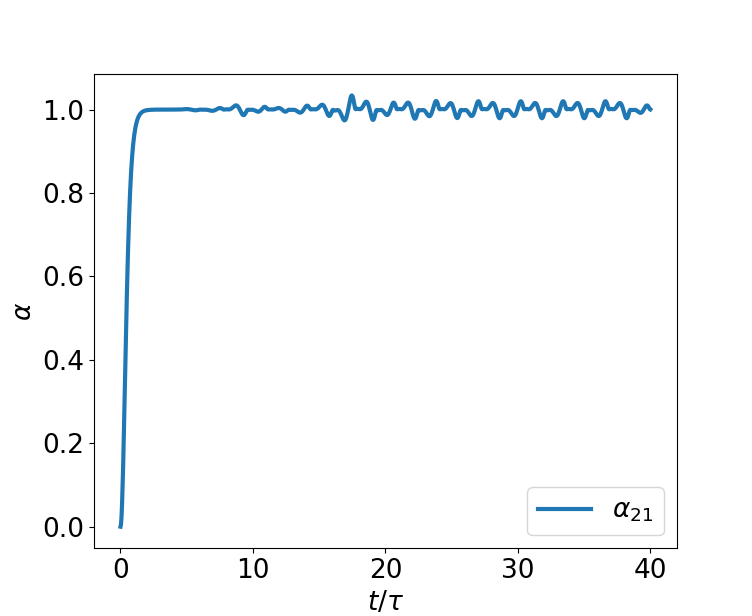
\includegraphics[width=0.48\textwidth]{alpha21_large_tmax.png}}
    \label{fig:a21_numeric}
\end{figure}

\noindent На \autoref{fig:a21_numeric} добре се вижда поведението на числения интегратор. При смяна на метода с такъв с по-сложно поведение (автоматично засичане на неустойчивост и съответен избор на стъпката) резултатите също са аналогични. Резултатът е добър и поведението е ,,хубаво`` за относително широк интервал от времена (в случая на  \autoref{fig:a21_numeric} до около $t_{max}/\tau = 10$, след което численият метод за интегриране става немонотонен. Причината за това е, че $\alpha$ при $t_{max}/\tau = 2$ е на практика достигнало равновесното $\alpha = 1$. От там нататък, разликите на всяка стъпка $\Delta \alpha$ са много малки - от порядъка на машинната грешка $\approx 10^-16$ и това води до наблюдаваното немонотонно поведение.

След числени експерименти за целите на крайната имплементация е избран методът \textit{DOP853} пред \textit{RK45}, тъй като контролът на неустойчивостта  е по-добър и немонотонността се проявява при по-големи $t/\tau$. Използването на методи с адаптивен избор на стъпката ни позволява да интегрираме с малка стъпка само в интервалите, където функцията нараства бързо и да контролираме алгоритъма чрез зададена отнапред относителна грешка.

Този проблем е неизбежен, независимо от метода за интегриране на ОДУ, който използваме но и не е толкова съществен предвид, че експериментите, за които искаме да правим параметрична идентификация на модела, рядко стигат до $\alpha \gg 90\%$. Все пак е важно този ефект да бъде взиман под внимание, когато се разработват оптимизационните методи за намиране на параметрите от експериментални данни, тъй като ,,началото`` на немонотонното поведение - зависи от $D, g, \tau$ и може да се окаже за по-малки $t/\tau$ от представените тук.

Тъй като за $\alpha_{21}$ имаме аналитично решение в затворен вид, можем да изчислим максималната и средната абсолютната грешка за даден интеграционен интервал, например $t/\tau \in [0, 2]$. На \autoref{fig:abs_error_a21} е представена графика на грешката за целия интервал. Очаквано, най-голяма е грешката в инфлексната точка $t/\tau = 0.329$, тъй като там и нарастването на функцията е най-голямо. При направената имплементация максимумът е $8\cdot10^{-9}$, докато средната грешка за интервала е $2\cdot10^{-9}$. 

\begin{figure}[hbtp]
    \centering
    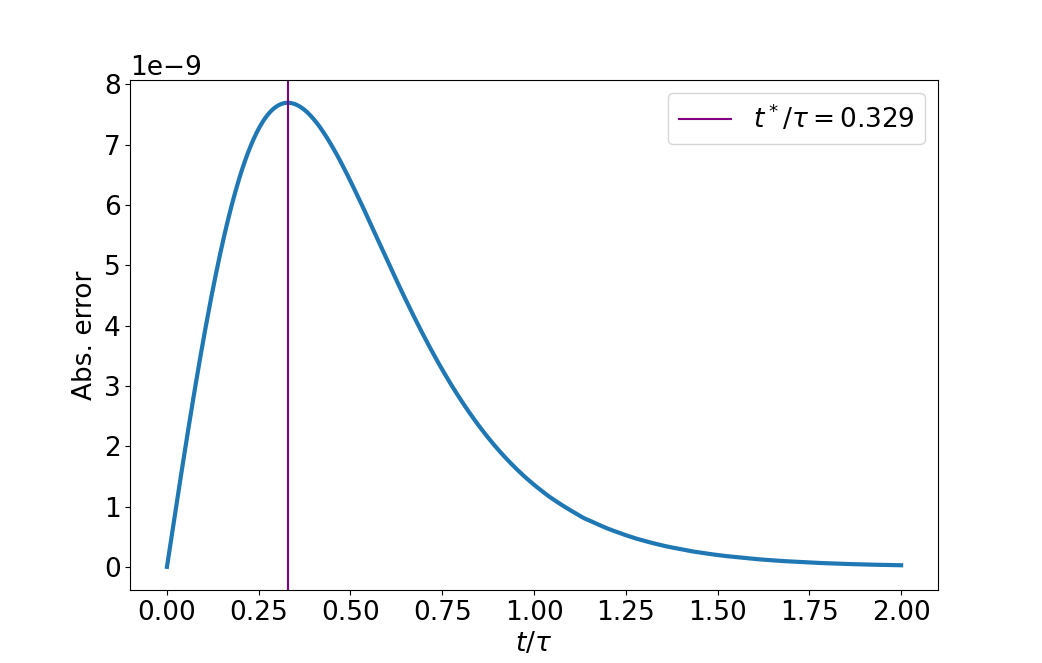
\includegraphics[width=\textwidth]{alpha21_abs_error.png}
    \caption{Абсолютна грешка от численото интегриране за $\alpha_{21}$}
    \label{fig:abs_error_a21}
\end{figure}

\subsubsection{Параметрична идентификация}
\label{subsub:parametric_identification}
Част от целите, които това изследване си поставя, е ,,инструментализацията`` на разработения модел, т.е. разработка на обща процедура, която да позволява от експериментални данни (реални или от числен експеримент) да се определят $D$ (дали растящият кристал e едно, дву - или тримерен) и $g$ (дифузионен или кинетичен контрол). 

Допълнително от \autoref{eq:time_scale} е ясно, че времевата скала $\tau$ съдържа началната скорост $r_0(g)$, която пък съдържа температурната зависимост на процеса. Затова определянето и на $\tau$ с останалите два параметъра ще бъде част от процедурата за параметрична идентификация. За целта умножаваме двете страни на \autoref{eq:main_aDg_ode} с $\tau$ и ще работим с тази ,,полу-обезразмерена`` форма на основното ОДУ.

Следващите процедури надграждат над тези от \autoref{subsub:numeric_integration}, тъй като дясната страна на основното ОДУ е непрекъсната по параметрите $D, g, \tau$. Това позволява да работим със стандартни подходи за параметрична идентификация за непрекъснати функции и по тази причина резултатите от оптимизацията ще са реални числа, а не цели. 

Тъй като ние целим да запазим физичния смисъл на параметрите $D, g$ резултатите от оптимизацията ще служат само за насока за режима на растеж и избор на правилната крива от \autoref{sub:analytic_results}. Параметри получени от оптимизацията, които не отговарят на предположенията поставени при извеждането ще разглеждаме като невъзможност на модела да обясни конкретния експеримент. 

За целите на следващите два параграфа ще въведем следната дефиниция:
\begin{definition}{Вектор на остатъците}{resd_vector}
    Ще предполагаме, че имаме $N$ експериментални точки $(t^{i}, \alpha^i)$ за $i = 1,...,N$. Ще отбележим с $\alpha_{D,g,\tau}^i$ стойността на $\alpha_{D,g,\tau}(t^i)$ при конкретен избор на параметрите $D, g, \tau$. Векторът на остатъците $\varepsilon$ тогава дефинираме като:
    \begin{equation*}
        \label{eq:resd_vector}
        \varepsilon(D, g, \tau) = \left( \alpha^1 - \alpha_{D,g,\tau}^1, \alpha^2 - \alpha_{D,g,\tau}^2,  ..., \alpha^N - \alpha_{D,g,\tau}^N \right)
    \end{equation*}
\end{definition}
\noindent Тогава общата оптимизационна задача, която ще решаваме е:
\begin{equation}
    \label{eq:optmiz_problem}
    (D^*, g^*, \tau^*) = argmin_{(D, g, \tau)} \lVert \varepsilon(D, g, \tau) \rVert
\end{equation}

\paragraph{Нелинейни най-малки квадрати (NLSQ)} Тук нормата, с която определяме големината на вектора на остатъците е втората норма $\lVert \cdot \rVert_{2}$:
\begin{equation*}
    \lVert  \varepsilon \rVert_{2} = \sqrt{\sum_{i} | \varepsilon_i| ^ 2}
\end{equation*}
Така получаваме класическата задача за нелинейни най-малки квадрати. Тъй като това е достатъчно добре изучена задача и броят експериментални точки е малък ($<20$) особено подходящ е алгоритъмът на \textit{Levenberg-Marquard} като модификация на алгоритъма на \textit{Gauss-Newton} с доверителна област. \cite{Kelley1999} 

Имплементация на \textit{Levenberg-Marquard} може да бъде намерена в пакета \textit{MIN\-PACK} за \textit{Fortran} \cite{MinpackGH}. Тази импле\-мен\-та\-ция е доказано ,,добра`` и ши\-ро\-ко\-изпол\-звана с различни опции като пресмятане на матрицата на Якоби чрез алгоритмично диференциране. Особено удобно е, че модулът \textit{Optimize} от \textit{SciPy} предоставя програмен интерфейс за \textit{Python} към \textit{MINPACK} \cite{2020SciPy-NMeth}. Този интерфейс се нуждае единствено от функцията, която пресмята вектора на остатъците $\varepsilon(D,g,\tau)$, начално предположение за стойността на параметрите и по желание на потребителя - експлицитни граници за параметрите и доверителната област.

Най-общо функцията за параметрична идентификация за произволен списък от експериментални точки $(t^{i}, \alpha^i)$ изглежда така:
\begin{minted}{python}
def fit_data(dat):
    fit = optimize.least_squares( # from the scipy module optimize
        lsq_cost, # function that calculates resds vec for given params
        x0=[
            FINDER_CONFIG["d_ini"],
            FINDER_CONFIG["g_ini"],
            FINDER_CONFIG["tau_ini"],
        ],
        args=(dat,),
        verbose=2,
        bounds=(
            (
                FINDER_CONFIG["d_min"],
                FINDER_CONFIG["g_min"],
                FINDER_CONFIG["tau_min"],
            ),
            (
                FINDER_CONFIG["d_max"],
                FINDER_CONFIG["g_max"],
                FINDER_CONFIG["tau_max"],
            ),
        ),
    )
    d = fit.x[0]
    g = fit.x[1]
    tau = fit.x[2]
    return fit, d, g, tau
\end{minted}

Конкретната имплементация с допълнително филтриране на данни, които са извън интеграционния интервал (с цел избягването на екстраполация) и команден интерфейс за работа с \textit{.csv}-файлове може да бъде намерена в скрипта \textit{parameter_finder.py} от \cite{SigmoidToolsGH}.

\paragraph{Равномерно приближение (uniform/minimax)} Тук искаме да минимизираме безкрайност нормата на вектора на остатъците $\lVert \cdot \rVert_{\infty}$:
\begin{equation*}
    \lVert \varepsilon \rVert_{\infty} = \max_{i} | \varepsilon_i| 
\end{equation*}
От общата теория е известно, че безкрайност нормата не е непрекъснато диференцируема и съответно градиентни методи за минимизирането ѝ не са подходящи. Не съществува и обобщен алгоритъм като \textit{Levenberg-Marquard} за решаването на тази задача.

Въпреки тези проблеми, намирането на най-доброто равномерно приближение е интересно практически, защото гарантира, че за дадени параметри на модела, максималната грешка не надвишава определена стойност.

За да намерим минимума на тази норма ще използваме модификация на Монте Карло метода на Метрополис, т.нар. \textit{симулирано закаляване}. Общият алгоритъм е много прост \cite{wiki:Simulated_annealing} и е необходимо целевата функция да е само $C^0$-непрекъсната:
\begin{algorithm}
\caption{Симулирано закаляване}\label{alg:cap}
    \begin{algorithmic}[1]
    \State $p \gets p_0$ \Comment{Начално предположение}
    \While{$k < k_{max}$} \Comment{Максимален брой итерации $k_{max}$}
        \State $T \gets Temperature (k)$
        \State $p_{new} \gets Neighbour(p)$
        \If{$\mathcal{P}\left(E(p), E(p_{new}), T\right) \ge RandomUniform(0,1)$}
            \State $p \gets p_{new}$
        \EndIf
    \EndWhile
    \State $ \text{\textbf{output}}~~p$
    \end{algorithmic}
\end{algorithm}

За конкретната имплементация е необходимо да бъдат дефинирани: началния вектор от параметри $p_0$, целевата функция $E(p
)$, функция с която да избираме следващия кандидат: $Neighbour(p)$, как понижаваме температурата на стъпка $k$ - $Temperature (k)$ и дискриминативна функция $\mathcal{P}\left(E(p), E(p_{new}), T\right)$, спрямо която решаваме дали запазваме новите параметри (напр. Болцманово разпределение в класическия алгоритъм на Метрополис). За симулирането закаляване можем да обобщим следното:
\begin{itemize}
    \item Това е глобална оптимизационна процедура.
    \item Стохастичен (случаен) метод.
    \item Успешността на алгоритъма \textit{силно} зависи от изброените по-горе функции.
\end{itemize}
Поради тези особености, съществуват разработени множество конкретни реализации - различни енергетични разпределения, рестартиране на алгоритъма, множество различни стартове комбинирани с локално търсене и т.н.  \cite{Xiang1997} \cite{Xiang2013}
В \textit{SciPy} модула \textit{Optimize} е направена имплементация на симулирано закаляване под името \textit{scipy.optimize.dual_annealing()} на база \cite{Xiang2013}, където за $Neighbour(p)$ е избрано например разпределението на Коши-Лоренц. Крайният интерфейс се нуждае единствено от целева функция, начално предположение и граници за всеки от параметрите. Допълнителни опции като избор на максималния брой итерации $k_{max}$ също са налични.

Най-общо функцията за параметрична идентификация за произволен списък от експериментални точки $(t^{i}, \alpha^i)$ изглежда така:
\begin{minted}{python}
def fit_data(dat):
    fit = optimize.dual_annealing(uniform_cost,
    x0 = (FINDER_CONFIG["d_ini"], 
    FINDER_CONFIG["g_ini"], 
    FINDER_CONFIG["tau_ini"]
    ), 
    bounds=((FINDER_CONFIG["d_min"], FINDER_CONFIG["d_max"]), 
            (FINDER_CONFIG["g_min"], FINDER_CONFIG["g_max"]),
            (FINDER_CONFIG["tau_min"], FINDER_CONFIG["tau_max"])),
    args=(dat,),
    )

    d = fit.x[0]
    g = fit.x[1]
    tau = fit.x[2]
    return fit, d, g, tau
\end{minted}
Командния интерфейс за работа с \textit{.csv}-файлове може да бъде намерен в скрипта \textit{parameter_finder_uniform.py} от \cite{SigmoidToolsGH}.
\subsection{Верификация на модела спрямо JMAKn}
Моделът $\aDg$ има за цел да бъде физически осмислена в контекста на кристализация из разтвор алтернатива на JMAKn, затова ще направим подробно сравнение на двата модела и ,,верификация`` на  $\aDg$ спрямо JMAKn.
С цел последващото изложение и по-директна аналогия, ще запишем JMAKn във вида:
\begin{equation}
    \label{eq:jmakn_with_time_scale}
    \alpha(t) = 1 - \exp{\left[ - \left( \frac{2 t}{\tau_{JMAKn}} \right)^n \right]}
\end{equation}
Т.е. сме заместили в \autoref{eq:jmak}: $k = (2/\tau_{JMAKn})^n$, тъй като $\tau_{JMAKn}$ може да бъде толкова произволно колкото $k$ не сме променили общността на записа.
\subsubsection{Диференциална форма на JMAKn}
В литературата рядко може да бъде намерена диференциалната форма на JMAKn или ако е публикувана, то нейното извеждане не директно направено \cite{Avramov2005}. За целта ние ще започнем като получим скоростта на нарастване на степента на трансформация $d \alpha/d t$ за JMAKn. Първо решаваме \autoref{eq:jmakn_with_time_scale} за $t/\tau_{JMAKn}$:
\begin{equation*}
    t/\tau_{JMAKn} = \frac{1}{2}\left[ - \ln{\left( 1- \alpha \right)} \right]^{1/n}
\end{equation*}
и диференцираме по $\alpha$:
\begin{equation*}
    \frac{d \left( t/\tau_{JMAKn} \right) }{d \alpha} = \frac{\left[ - \ln{\left( 1- \alpha \right)} \right]^{\frac{1-n}{n}}}{2n(1-\alpha)}
\end{equation*}
заедно с теоремата за производна на обратната функция, получаваме:
\begin{equation}
    \label{eq:jmak_differential_form}
    \frac{d \alpha}{d (t/\tau_{JMAKn})} = 2n(1-\alpha)\left[ \ln{\left( \frac{1}{1-\alpha} \right)} \right] ^ {\frac{n-1}{n}}
\end{equation}
Дясната страна на това ОДУ за $n = 2$ може да бъде намерено формулирано като вероятностно разпределение за $\alpha$ в \cite{Stoyanov1988} \cite{Fanfoni1998}.

От този запис веднага се вижда съответствието с \autoref{eq:main_aDg_ode}. За $n = 1$ дясната страна изцяло съвпада с тази на $\alpha_{11}$, както и интегралната крива от \autoref{eq:jmak_time_scale} и тази за $\alpha_{11}$ от \autoref{sub:analytic_results}.

\noindent Нещо повече, нека вземем предвид следния ред на Тейлър развит около $\alpha = 0$:
\begin{equation}
    \ln{\left( \frac{1}{1-\alpha} \right)} = \sum_{k=1}^\infty \frac{\alpha^k}{k}, \qquad |\alpha| < 1
\end{equation}
И развием логаритъма в скобите от \autoref{eq:jmak_differential_form} взимайки само линейният член ($k=1$), получаваме:
\begin{equation}
    \label{eq:jmakn_power_series}
    \frac{d \alpha}{d \left( t/\tau_{JMAK} \right)} = 2 n \alpha^{\frac{n-1}{n}}\left(1-\alpha\right) + O(\alpha^{^{\frac{2(n-1)}{n}}})
\end{equation} %% TODO: check power
Тогава за \textbf{малки} степени на превръщане ($\alpha \approx 0$): $\aDg$ и JMAKn съвпадат с $D = n$, $g = 1$ и $\tau_{JMAKn} = \tau_{D1}$.

\subsubsection{Инфлексни точки на JMAKn}
В литературата е разпространена $\left\{t^*/\tau_{JMAKn};\alpha^* \right\} = \left\{1/2; 1 - 1/e \right\}$ \cite{Avramov2005} като единствена инфлексна точка на JMAKn, която не зависи от избора на $n$. Това очевидно няма как да бъде вярно, особено предвид че при $n = 1$ такава инфлексна точка не съществува (отново има само отрицателна обратна връзка).
Следвайки процедурата в \autoref{sub:aDg_infl_points} можем аналогично да получим за инфлексната точка на JMAKn при конкретен избор на $n$:
\begin{equation}
    \label{eq:jmak_infl_point}
     \left\{ t^* / \tau_{JMAKn}; \alpha^* \right\}  = \left\{\frac{1}{2} \left( \frac{n-1}{n} \right); 1-e^{\frac{1}{n} - 1}\right\}
\end{equation}
Ако в \autoref{eq:jmak_infl_point} пуснем $n \rightarrow \infty$ в дясната страна ще получим именно $\left\{1/2; 1 - 1/e \right\}$.
Можем и да изключим $n$, за да получим директно имплицитна крива за $\alpha^*$ свързваща двете координати на инфлексната точка:
\begin{equation*}
    t^*/\tau_{JMAKn} (\alpha ^ *) = \frac{1}{2}\left( \ln{\left( \frac{1}{1-\alpha^*} \right)} \right)^{1+\ln{(1-\alpha^*)}}, \qquad 0 < \alpha^* \le  1 - 1/e 
\end{equation*}
В \autoref{tabl:jmak_infl_points} са представени обобщено инфлексните точки за избрани стойности на $n$, които могат да бъдат срещнати често в литературата. Допълнително на \autoref{fig:infl_points_curves} са представени параметричните криви, даващи инфлексните точки на JMAKn, $\alpha_{D1}$  и $\alpha_{D2}$ при вариране на $D$ или $n$. Кривата за \textcolor{green}{JMAKn} е винаги над правата $\alpha^* = t^*$, докато $\aDg$ я пресичат. Трябва да се има предвид, че с тези криви следва да се работи внимателно, защото за дадена точка от тях не е директно очевидно на каква стойност на параметрите отговаря. От друга страна те могат да служат за ориентир за ,,близостта`` на моделите при тези различни параметри - например се вижда, че $\alpha_{21}$ e най-близо до JMAKn за $n = 1.725$, вместо $n = 2$.

\begin{table}[hbpt]
\centering
\resizebox{\textwidth}{!}{%
\begin{tabular}{ccccccc}
\hline
\textbf{n}                                     & \textbf{1} & \textbf{1.725}    & \textbf{2}         & \textbf{2.43}     & \textbf{3}        & \textbf{4}        \\ \hline
$\left\{(t^*/\tau_{JMAK_n}); \alpha^*\right\}$ & -          & $\{0.303;0.343\}$ & $\{0.354; 0.393\}$ & $\{0.402;0.445\}$ & $\{0.437;0.487\}$ & $\{0.465;0.528\}$ \\ \hline
\end{tabular}%
}
\caption{Инфлексни точки на JMAKn при различни стойности на $n$}
\label{tabl:jmak_infl_points}
\end{table}
\begin{figure}[hbtp]
    \centering
    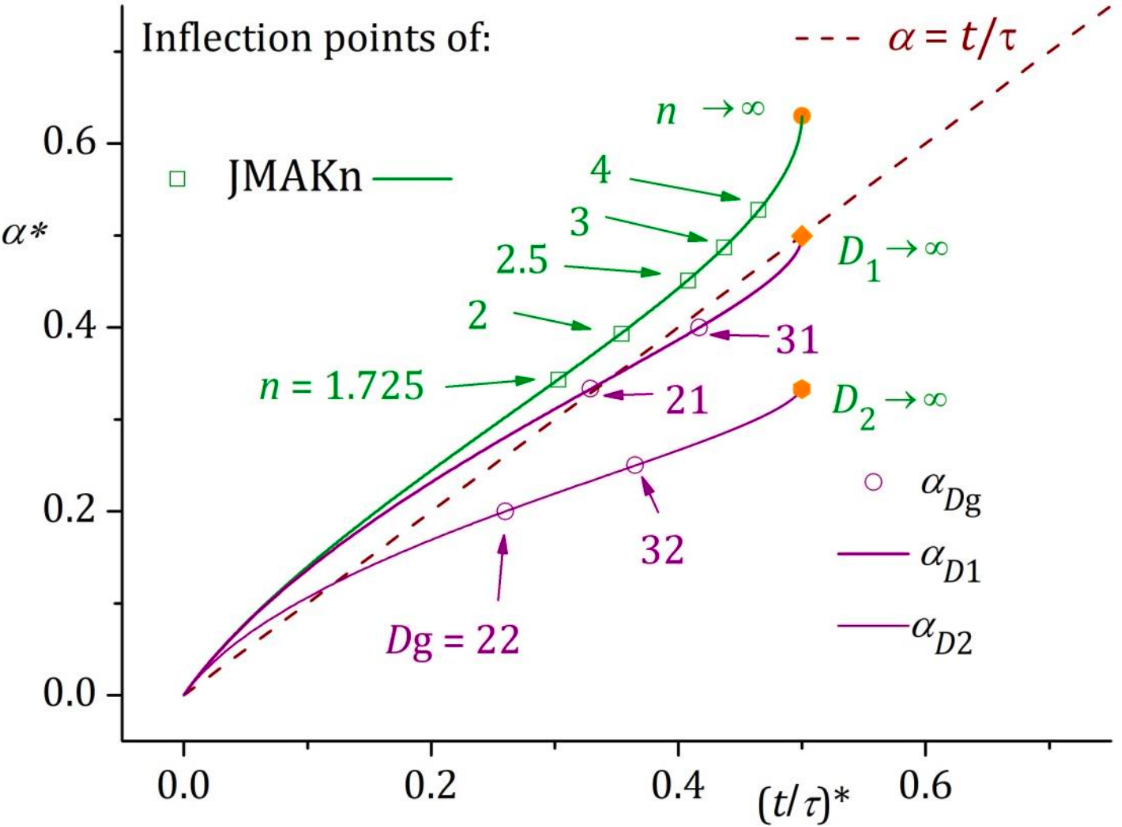
\includegraphics[width=0.80\textwidth]{adg_jmakn_infl_points.png}
    \caption{Инфлексни точки на JMAKn и $\aDg$ при различни стойности на параметрите}
    \label{fig:infl_points_curves}
\end{figure}
\subsubsection{Числено сравнение (фитване) на JMAKn и \texorpdfstring{$\aDg$}{αDg}}
Тук ще използваме процедурите разработени в \autoref{subsub:parametric_identification} за да намерим кои параметри на $\aDg$ водят до крива най-близо (метрично) до $JMAKn$ за дадено $n$ и обратно - кой избор на $n$ води до JMAKn крива най-близо до $\alpha_{D1}$ за дадено $D$.
\autoref{eq:jmakn_power_series} показва, че двата модела са близки за малки $\alpha$ при съответен избор на параметрите, затова в този параграф ще генерираме гъста мрежа от точки ($\Delta t < 0.001$) и стойности, така че $\alpha \in [0, 0.999]$ от единия модел и ще го ,,фитнем`` с другия с \textit{NLSQ} (JMAKn и $\aDg$) и \textit{Uniform} (JMAKn). Тъй като $\alpha_{11}$ съвпада аналитично с JMAK1, най-интересни ще са ни стойностите за  $D \ge 2$.  По този начин ще получим представа в по-широк интервал как биха и до колко си съответстват двата модела.  

Като начало въвеждаме безразмерен конверсионен фактор между двете скали, за да можем по-удобно да покажем разликата между тях. Можем и да въведем по-сложна зависимост между скалите, но това трудно би било оправдано, предвид че за малки $\alpha$ двете трябва да съвпадат точно.
\begin{equation*}
    \tau_{JMAKn} = c_{f} \tau_{Dg}
\end{equation*}

\paragraph{Фитване на $\aDg$ с JMAKn}
Ще започнем като намерим за $\alpha_{21}$ и $\alpha_{31}$ по NLSQ кое е това $n$, за което е най-близка съответната JMAKn-крива. На \autoref{fig:fit_adg_with_jmakn} са представени тези резултати. За конверсионния фактор получаваме $c_{f} \approx 1.1$. Т.е. дори в този широк интервал двете времеви скали са относително близки. Разликите са по-скоро в $D$ и $n$, които са значими, особено предвид че това са експоненти в изразите.
\begin{figure}[hbpt]
    \centering
    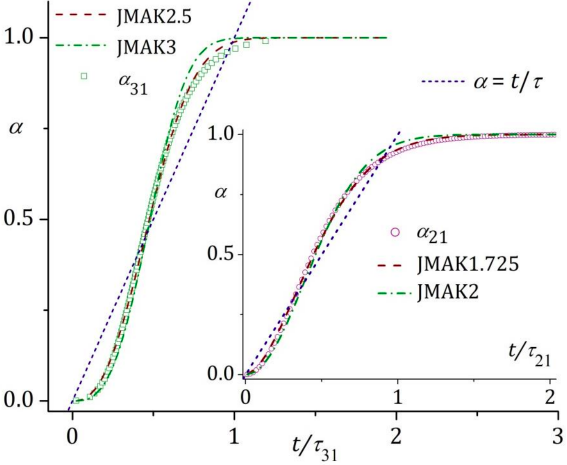
\includegraphics[width=0.8\textwidth]{alpha21andalpha31vsjmak.png}
    \caption{Фитване на $\alpha_{31}$ (основна фигура) с JMAK2.5 и $\alpha_{21}$ с JMAK1.725 (вложена)}
    \label{fig:fit_adg_with_jmakn}
\end{figure}
Същите две графики ще представим и в т.нар. Аврами координати (двойно логаритмични), в които моделът JMAKn се линеаризира. Тези координати са били исторически важни за параметрична идентификация на модела, тъй като тогава не е необходимо да се решава задачата за нелинейни най-малки квадрати. \cite{Fanfoni1998} Линеаризацията изглежда така: 
\begin{equation*}
    \ln{\ln{\left(\frac{1}{1-\alpha}\right)}} = \ln{\left(\frac{t}{\tau_{JMAKn}}\right)}
\end{equation*}
\begin{figure}[!ht]
    \centering
        \caption{Фитване на $\aDg$ с JMAKn в Аврами координати}
        \subfloat[$\alpha_{21}$]{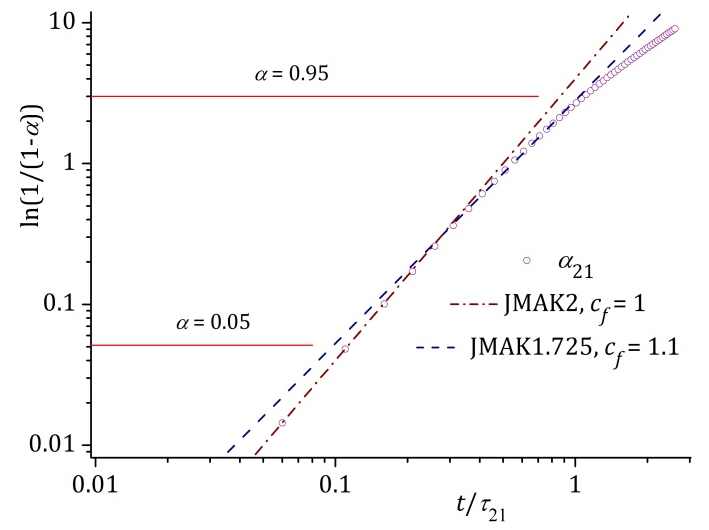
\includegraphics[width=0.48\textwidth]{avramia21.png}}
        \subfloat[$\alpha_{31}$]{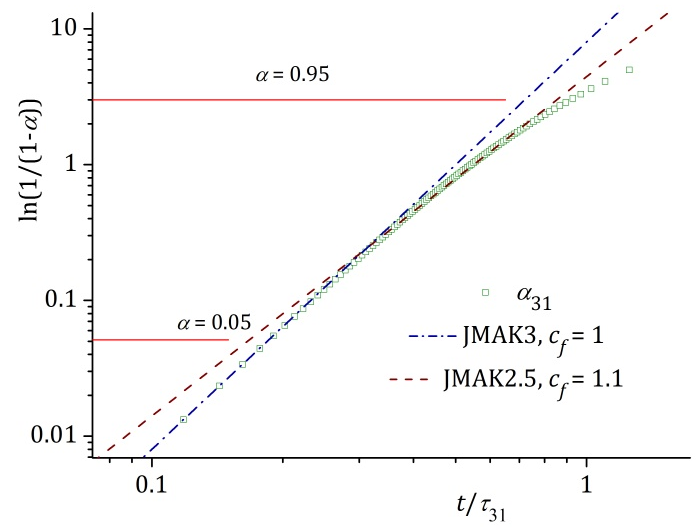
\includegraphics[width=0.48\textwidth]{avramia31.png}}
    \label{fig:avrami_coords_adg_jmak}
\end{figure}
Да обърнем внимание, че в Аврами координати заради нелинейността на осите, малки отклонения всъщност могат да са значителни в линейни координати. Интересен е и ,,десният завой`` на $\aDg$ моделите от JMAKn при големи степени на трансформация.
\begin{figure}[!ht]
    \centering
        \caption{Фитване на $\aDg$ с JMAKn за различни стойности на $\alpha_{upper}$}
        \subfloat[$\alpha_{21}$]{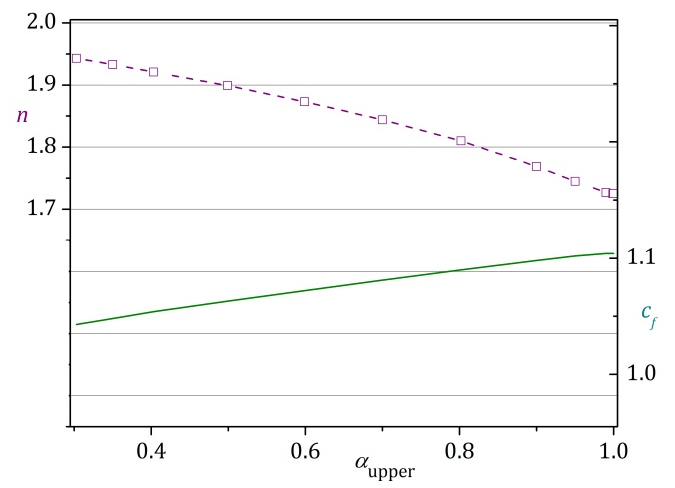
\includegraphics[width=0.48\textwidth]{avramia21_jmak_alphamax_change.png}}
        \subfloat[$\alpha_{31}$]{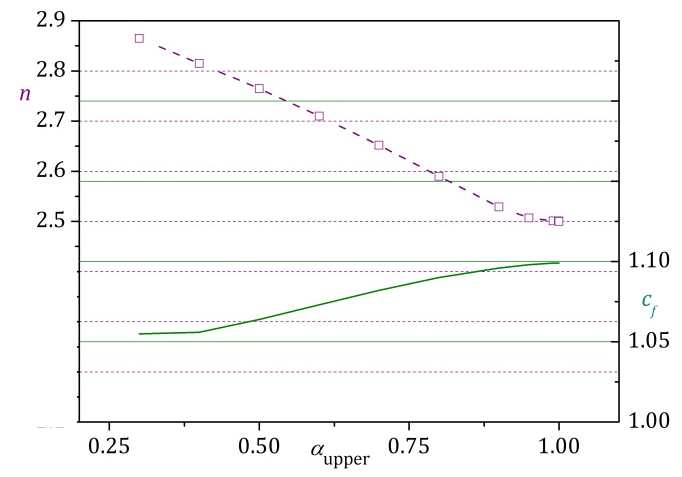
\includegraphics[width=0.49\textwidth]{avramia31_jmak_alphamax_change.png}}
    \label{fig:avrami_coords_adg_jmak_moving_alpha_max}
\end{figure}

На \autoref{fig:avrami_coords_adg_jmak_moving_alpha_max} са комбинирани идеите до тук, като са проведени параметрични идентификации. Данните генерирани от $\aDg$, са такива че $\alpha \in [0, \alpha_{upper}]$, като пък $\alpha_{upper} \in [0.1, 0.999]$. Така се вижда добре нарастването на разликата между $D$ и $n$, съответно и промяната на $c_{f}$ от $1$ до $\approx 1.1$.

От настоящия параграф и фигурите се очертава ясна картина - резултатите от параметричната идентификация зависят от размаха на данните по $\alpha$. Това означава, че трябва внимателно да боравим с експериментални измервания за степента на превръщане, особено когато процесът не е доведен докрай, тъй като тази зависимост от $\alpha_{upper}$ може да скрие ,,истинския`` модел описващ данните. 
%% TODO: interpolate
Глобално оптималните параметри ($\alpha_{upper} \approx 1$) водят до крива, която е метрично близка (в $\lVert \cdot \rVert_{2}$-норма) до съответната $\aDg$, но не я интерполира в $\alpha \rightarrow 0$. Обратно, развитието в ред на Тейлър от \autoref{eq:jmakn_power_series} е много близо до $\aDg$-кривата в началото, но разликата нараства значително с нарастване на $\alpha$.
\paragraph{Фитване на JMAKn с $\aDg$} Ще използваме процедурите разработени в \autoref{subsub:parametric_identification} за да направим параметрична идентификация за данни генерирани от JMAKn при $\alpha \in [0, 0.9999]$. Ще фиксираме $g = 1$ и ще оставим само $D$ и $c_{f}$ да получим като резултат от оптимизацията. Получените параметри са обобщени в \autoref{tabl:fit_jmak_with_adg}.
\begin{table}[hbtp]
\centering
\resizebox{0.7\textwidth}{!}{%
\begin{tabular}{@{}ccccc@{}}
\toprule
\textbf{n от JMAKn}            & \textbf{D}                    & $\boldsymbol{c_{f}}$               & $\boldsymbol{R^2}$                     & \textbf{Процедура}              \\ \midrule
                                 & 1.002                         & 1.00026                        & 0.9999992                          & NLSQ                            \\
\multirow{-2}{*}{\textbf{1}}     & \cellcolor[HTML]{EFEFEF}1     & \cellcolor[HTML]{EFEFEF}0.9999 & \cellcolor[HTML]{EFEFEF}0.99999998 & \cellcolor[HTML]{EFEFEF}UNIFORM \\
                                 & 1.989                         & 1.104                          & 0.9994                             & NLSQ                            \\
\multirow{-2}{*}{\textbf{1.725}} & \cellcolor[HTML]{EFEFEF}1.966 & \cellcolor[HTML]{EFEFEF}1.105  & \cellcolor[HTML]{EFEFEF}0.9993     & \cellcolor[HTML]{EFEFEF}UNIFORM \\
                                 & 2.371                         & 1.109                          & 0.9991                             & NLSQ                            \\
\multirow{-2}{*}{\textbf{2}}     & \cellcolor[HTML]{EFEFEF}2.352 & \cellcolor[HTML]{EFEFEF}1.110  & \cellcolor[HTML]{EFEFEF}0.9991     & \cellcolor[HTML]{EFEFEF}UNIFORM \\
                                 & 2.993                         & 1.105                          & 0.99883                            & NLSQ                            \\
\multirow{-2}{*}{\textbf{2.43}}  & \cellcolor[HTML]{EFEFEF}3.000 & \cellcolor[HTML]{EFEFEF}1.108  & \cellcolor[HTML]{EFEFEF}0.99882    & \cellcolor[HTML]{EFEFEF}UNIFORM \\
                                 & 3.073                         & 1.106                          & 0.99879                            & NLSQ                            \\
\multirow{-2}{*}{\textbf{2.5}}   & \cellcolor[HTML]{EFEFEF}3.036 & \cellcolor[HTML]{EFEFEF}1.107  & \cellcolor[HTML]{EFEFEF}0.99884    & \cellcolor[HTML]{EFEFEF}UNIFORM \\ \midrule
                                 & 3.794                         & 1.100                          & 0.99859                            & NLSQ                            \\
\multirow{-2}{*}{\textbf{3}}     & \cellcolor[HTML]{EFEFEF}3.801 & \cellcolor[HTML]{EFEFEF}1.102  & \cellcolor[HTML]{EFEFEF}0.99857    & \cellcolor[HTML]{EFEFEF}UNIFORM \\
                                 & 5.215                         & 1.083                          & 0.99828                            & NLSQ                            \\
\multirow{-2}{*}{\textbf{4}}     & \cellcolor[HTML]{EFEFEF}5.267 & \cellcolor[HTML]{EFEFEF}1.084  & \cellcolor[HTML]{EFEFEF}0.99829    & \cellcolor[HTML]{EFEFEF}UNIFORM \\ \bottomrule
\end{tabular}%
}
\caption{Резултати от фитването на JMAKn с $\aDg$ при фиксирано $g = 1$}
\label{tabl:fit_jmak_with_adg}
\end{table}

Двете задачи за най-малки квадрати не са напълно еквивалентни (от JMAKn да намерим параметрите на $\aDg$ и обратно). Близките резултати и в двата случая, показват че в най-общ смисъл $n = 1.725$ съответства на $D = 2$ и $n = 3$ на $D = 2.43$ за достатъчно голям размах на данните по степента на трансформация $\alpha$. Факторът $c_{f}$ и в двата случая е консистентно $\approx 1.1$. Така очертаваме съответствие между параметрите на двата модела, което ще е удобно за рационализиране на експериментални данни описани в литературата с JMAKn. 

За да обобщим казаното в този параграф можем да построим графика $n vs. D$ в интервала $2 \le D \le 3$. От \autoref{fig:nvsd_graph} се вижда, че тази зависимост е линейна. 
\begin{figure}[hbpt]
    \centering
    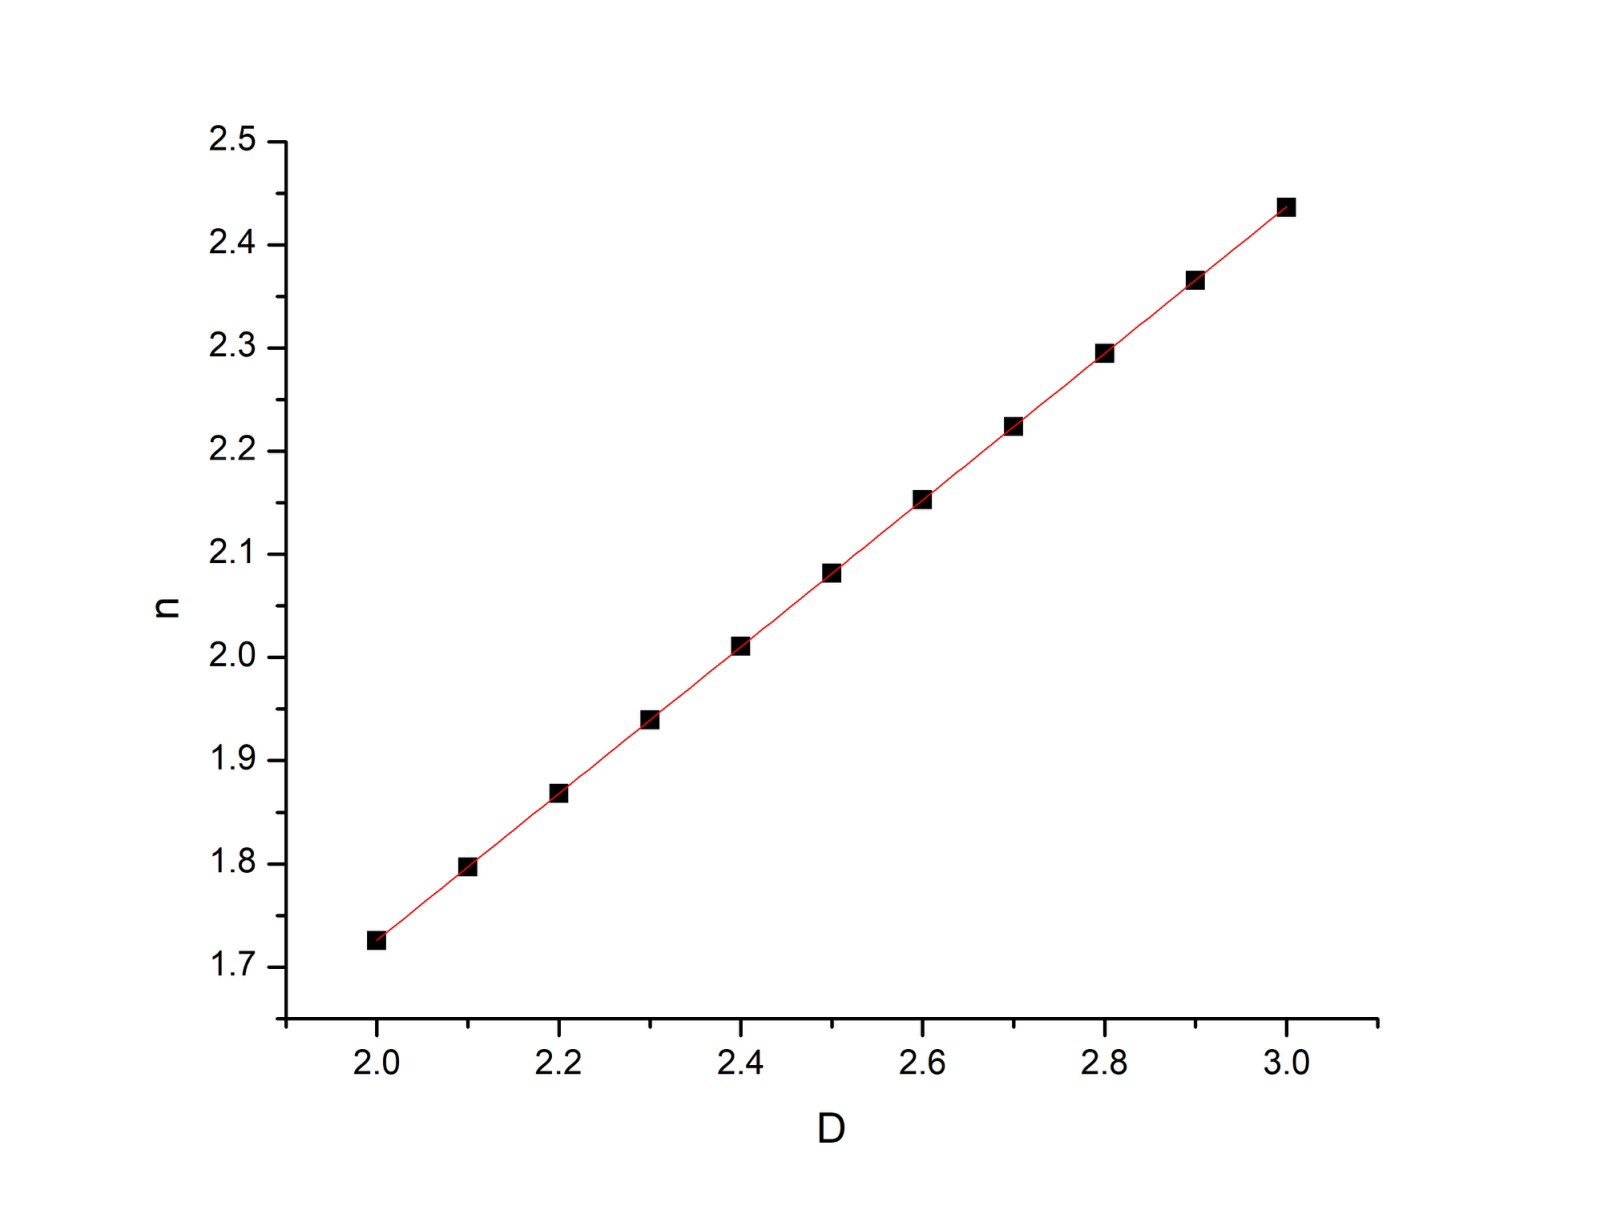
\includegraphics[width=\textwidth]{nvsd.png}
    \caption{Графика на съответствието между $D$ от $\aDg$ и $n$ от най-доброто метрично приближение с JMAKn. Уравнението на правата е $n  = 0.30385 D + 0.71106$} с коефициент на корелация: $R^2 \approx 1 - 1.31 \cdot 10^{-6}$.
    \label{fig:nvsd_graph}
\end{figure}
Като се замести $D = 1$ в уравнението на правата (екстраполация назад) от \autoref{fig:nvsd_graph} се получава $n = 1.01491$, което не е твърде голяма грешка спрямо истинската стойност, предвид че екстраполираме. В този смисъл това уравнение на права може да бъде полезен инструмент за ,,конверсия`` между двата модела.
\subsection{Валидиране с експериментални данни}
\label{sub:experimental_validation}
Основната цел, която си поставихме с този модел е да дадем алтернатива на JMAKn, чиито параметри да носят физически смисъл за целите на изотермична кристализация из разтвор. За да покажем, че това е така ще направим валидиране с реални експериментални данни.
За целите на тази секция ще се фокусираме върху експериментните проведени от \textit{Min, Sinclair, et. al.} \cite{Min2005}.  В  това изследване е използвана тунелна електронна микроскопия (ТЕМ) за изследване на кинетиката на кристализация на тънки $Ta_2O_5$-филми (стъкла) отлагани върху силициеви субстрати. Изследванията са проведени за три различни температури - $790^\circ~C, 820^\circ~C, 850^\circ~C$. Кристализацията при този експеримент е квази-двумерна (2D), тъй като самите тънки филми могат да се разглеждат като квази-двумерни обекти. За трите различни температури са получени стойности за $n$ в JMAKn съответно $n = 2.5, 1.9, 1.7$. Това означава, че няма как използвайки получените скали всички данни да бъдат прескалирани, така че да бъдат описани от една крива.

За да покажем предимствата на $\aDg$ ще използваме $\alpha_{21} = \tanh^2(2t/\tau)$ модела за всеки от трите набора експериментални данни от фиг. 7 на \cite{Min2005}. Ще използваме процедурата за нелинейни най-малки квадрати (NLSQ) за да определим съответните скали $\tau$.
\begin{figure}[hbpt]
    \centering
    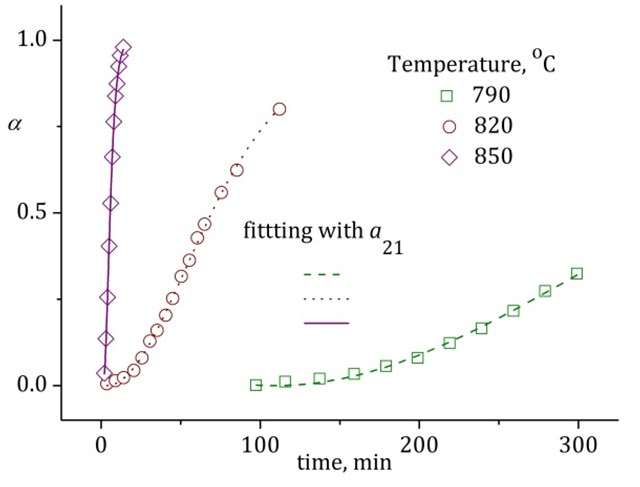
\includegraphics[width=0.83\textwidth]{min_3_curves.jpg}
    \caption{Данните от фиг. 7 на \cite{Min2005} и съответните криви с $\alpha_{21}$, с коефициент на корелация $R^2 = 0.996, 0.999, 0.999$ съответно.}
    \label{fig:a21_min}
\end{figure}

В процеса на параметрична идентификация за \autoref{fig:a21_min} получаваме скала за данните за всяка температура. Тези скали можем да използваме да преоразмерим времената от оригиналните данни. Така очакваме да получим единствена крива (т.нар. ,,master curve``) с безразмерни времена. Това ще потвърди разбирането, че режимът на растеж е един и същ и в трите случая, като данните се различават само по характеристичните времена на процеса (температурна зависимост).
\begin{figure}[hbpt]
    \centering
    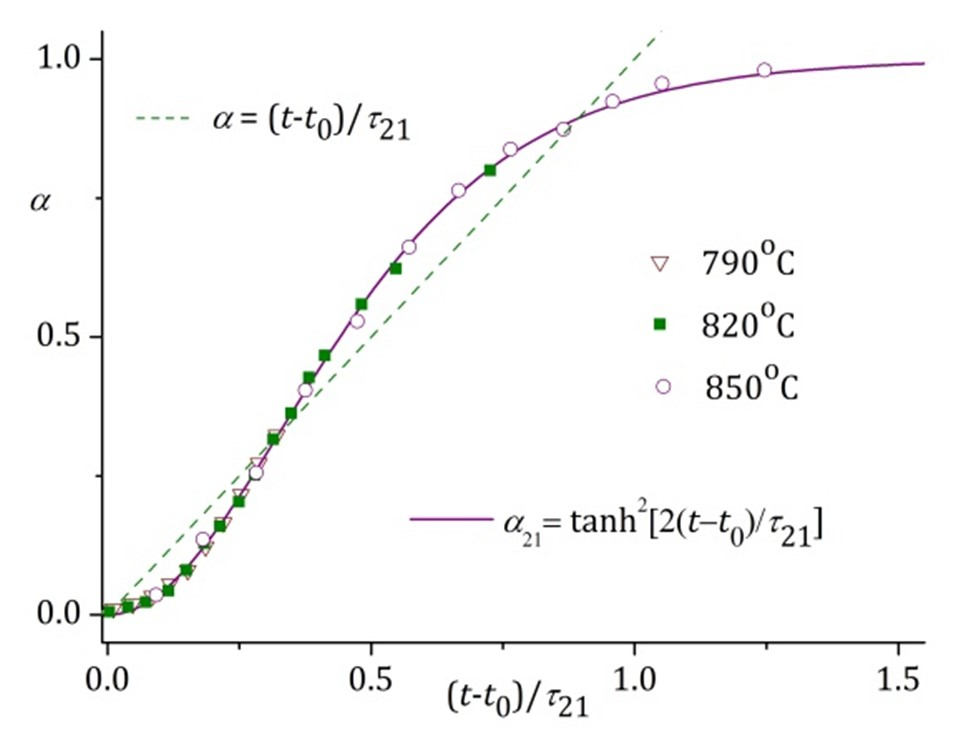
\includegraphics[width=0.65\textwidth]{min_a21_master_curve.jpg}
    \caption{Крива с рескалираните данни. Вижда се ясно как всички данни ,,лягат`` добре на една и съща крива, въпреки значително различни характеристични времена на процесите.} 
    \label{fig:a21_min_master_curve}
\end{figure}
\begin{figure}[hbpt]
    \centering
    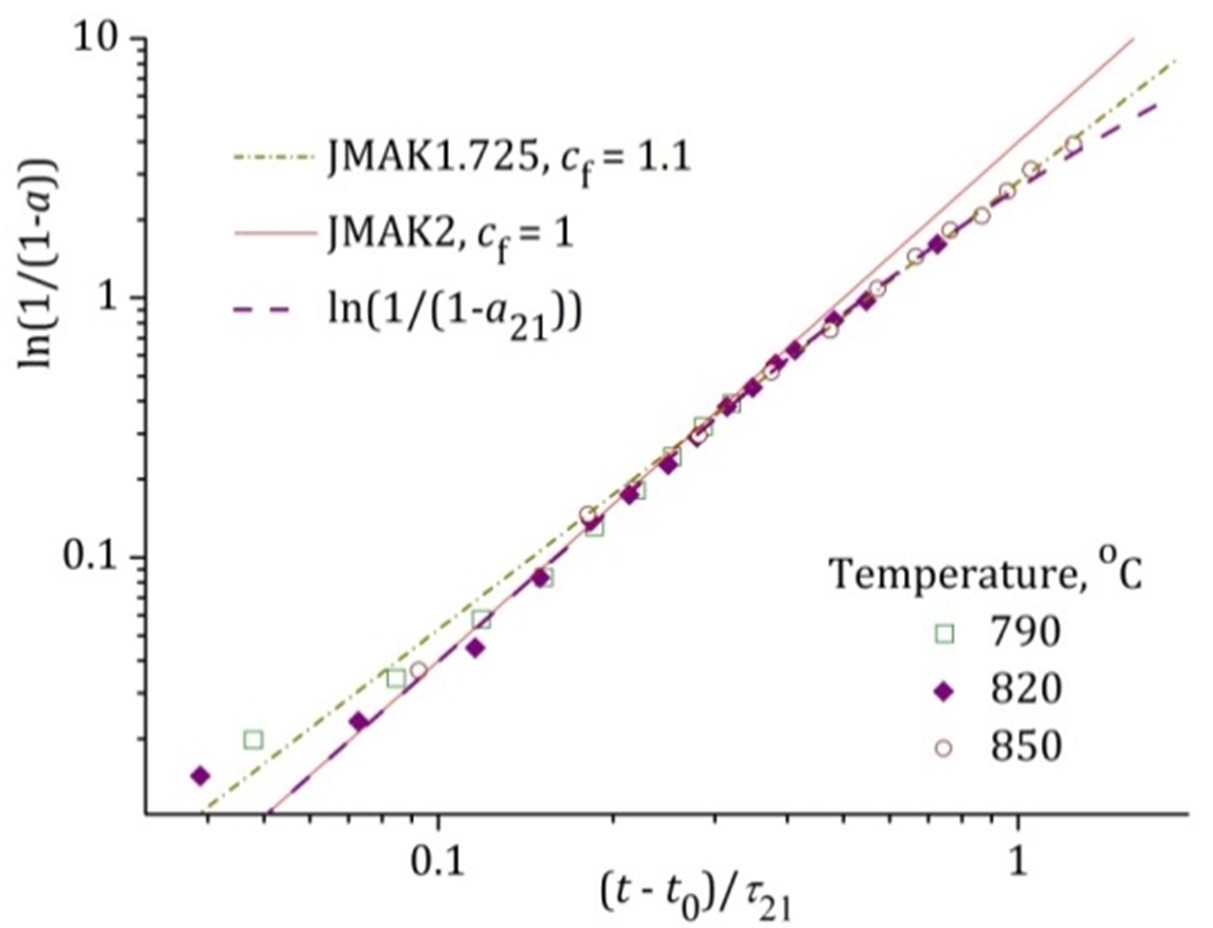
\includegraphics[width=0.65\textwidth]{min_a21_master_curve_avrami_plot.jpg}
    \caption{Крива \autoref{fig:a21_min_master_curve} представена в Аврами координати. Вижда се ясно как и при трите температури малките степени на трансформация не се описват добре от модела, но при големи $\alpha$ данните завиват надясно от JMAKn, което пък се описва добре от $\alpha_{21}$.}
    \label{fig:a21_min_master_curve_avrami}
\end{figure}

\subsection{Валидиране с данни от клетъчен автомат}
В областта на кристалния растеж един от инструментите за симулиране на физичния процес кристализация са клетъчните автомати. Те позволяват иначе сложният макроскопски процес да бъде моделиран чрез простите локални правила, които го обусловят. Един от най-първите микроскопски модели на електроотлагане на метали е така наречена дифузионно-лимитирана агрегация (DLA), чиито резултантни структури са познати като DLA-клъстери. 
\begin{figure}[hbpt]
    \centering
    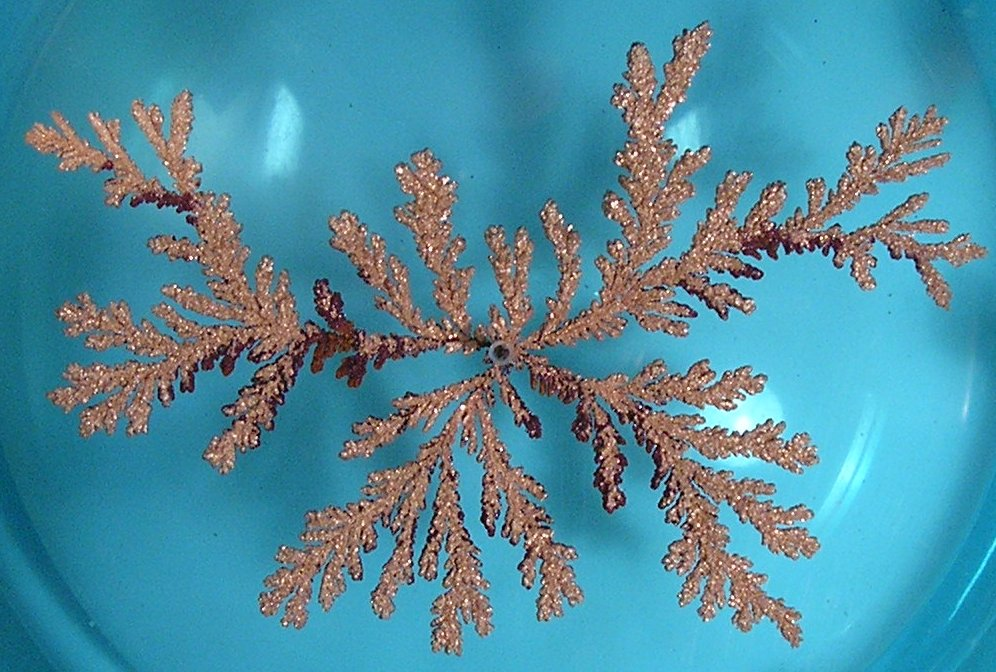
\includegraphics[width=0.65\textwidth]{dla_cluster_copper.jpg}
    \caption{DLA клъстер получен при електроотлагане на мед из разтвор на меден сулфат \cite{dla_copper}.}
    \label{fig:dla_cluster_wikimedia}
\end{figure}

Първият стохастичен (тип случайна разходка) модел на DLA е даден от \textit{Witten \& Sander} \cite{DLA_Witten}. В него започваме с агрегат от една частица (зародиша), спрямо която от ,,безкрайност`` дифундират останалите частици.
Когато една дифундираща частица пристигне при агрегата, тя се свързва необратимо като става част от него. Числената реализация на този модел има своите особености, тъй като условието за старт безкрайно далеч от агрегата е практически неизпълнимо. От друга страна, ако дифундиращите частици стартират твърде далеч от зародиша, симулациите са бавни, ако са твърде близо - предпоставки на модела се нарушават. В литературата са намерени практически решения на тези проблеми, като при симулация върху достатъчно голяма квадратна решетка се получават именно структури от вида на \autoref{fig:brownian_tree} - т.нар. браунови дървета.
\begin{figure}[hbpt]
    \centering
    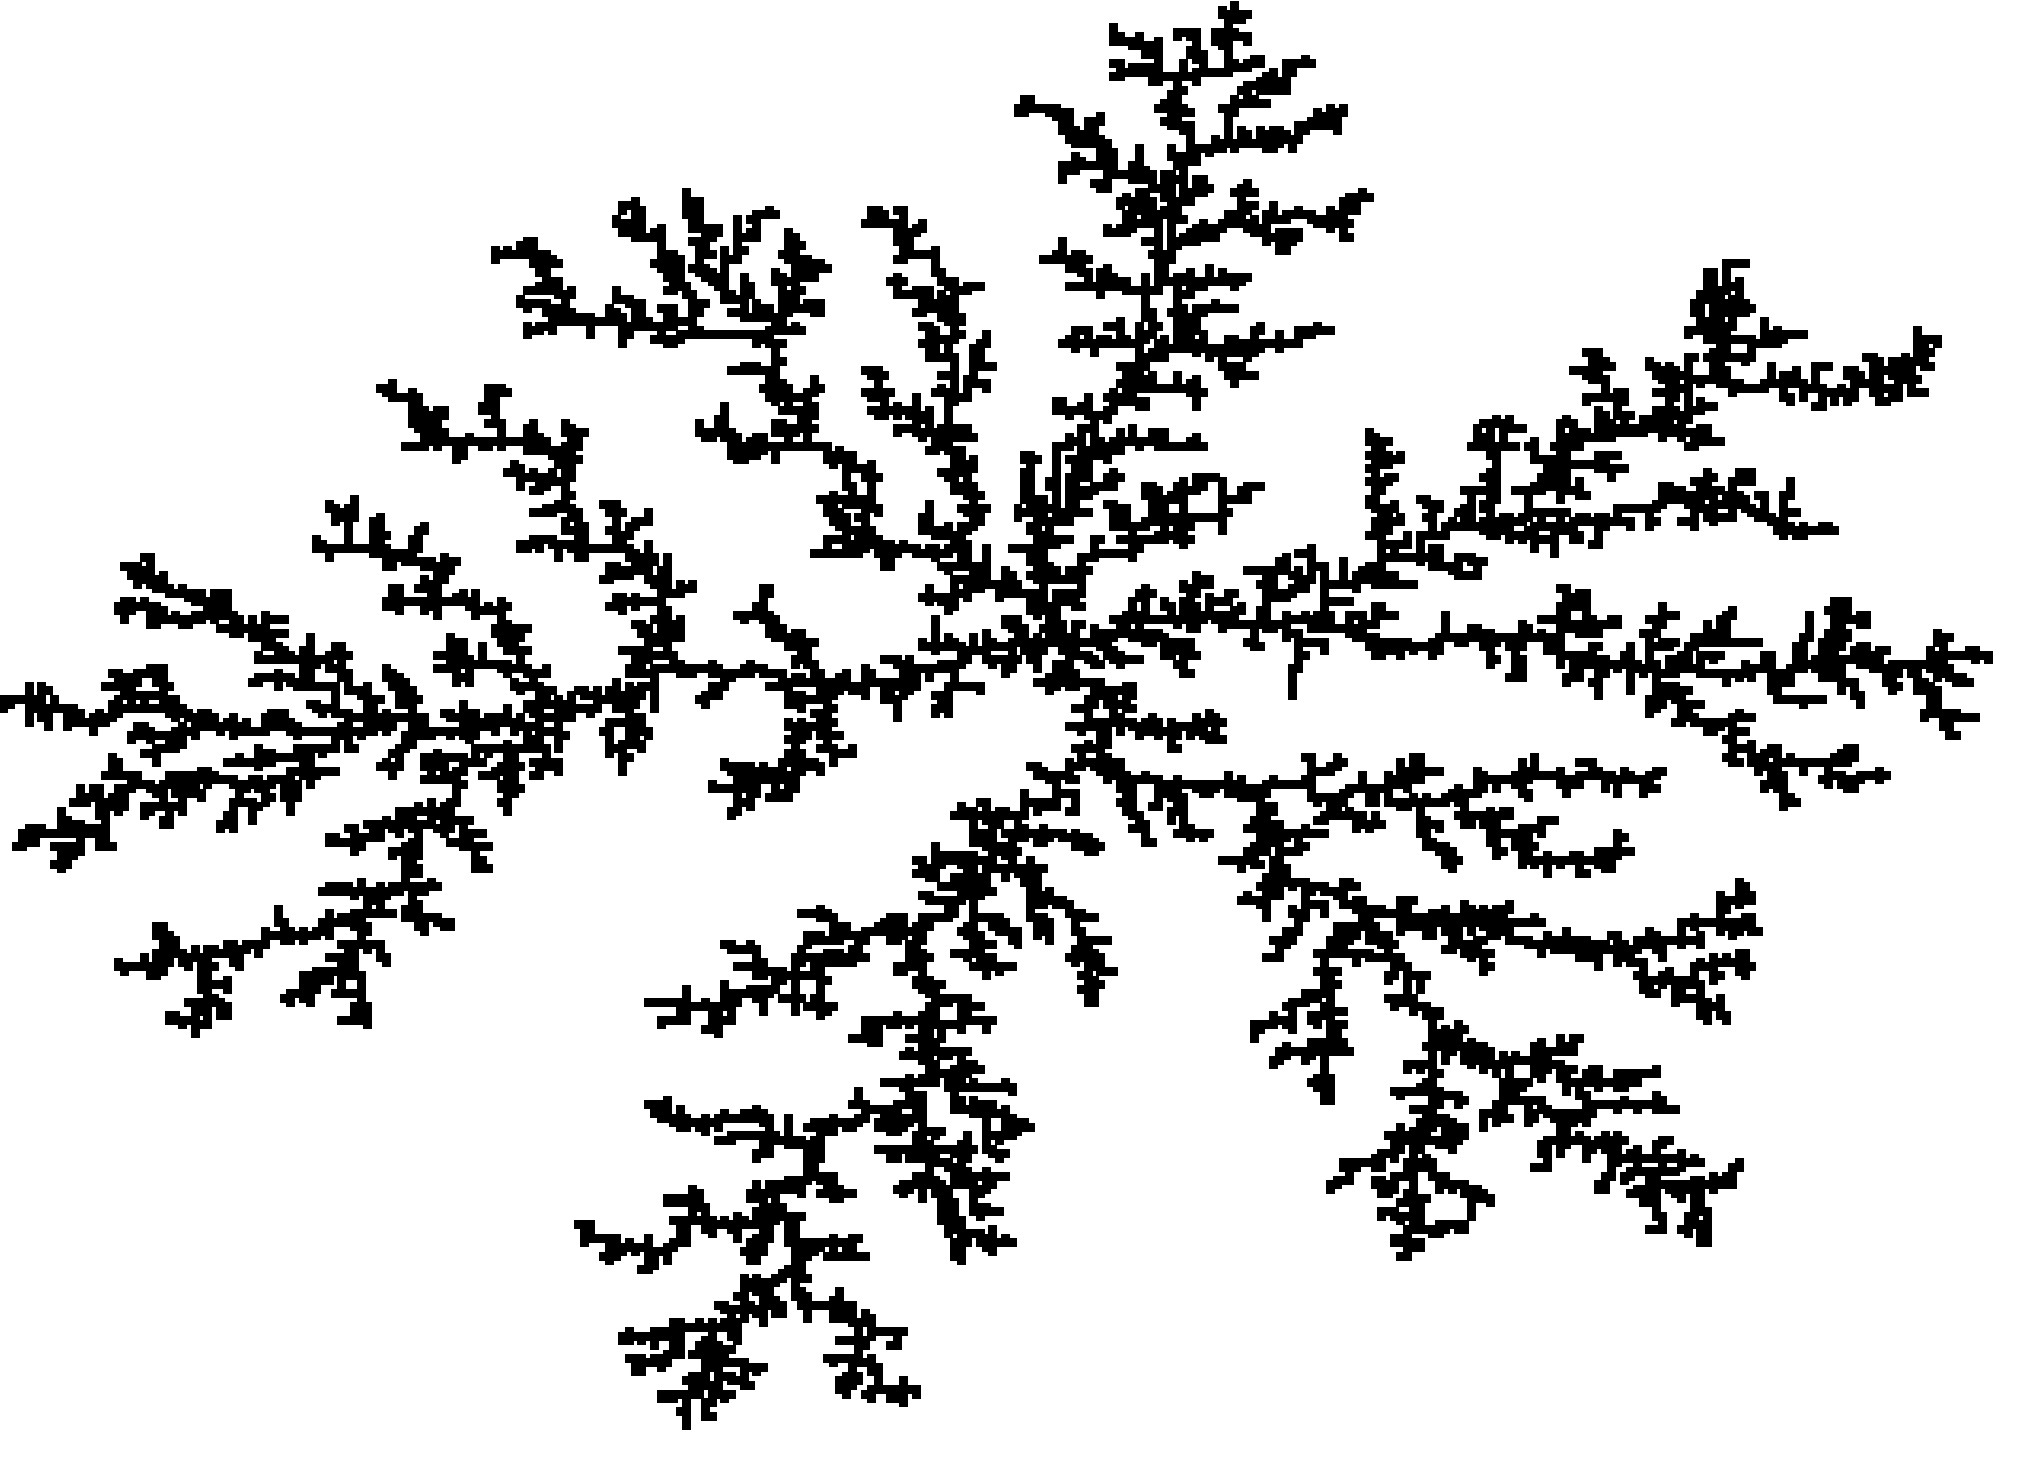
\includegraphics[width=0.65\textwidth]{brownian_tree.jpg}
    \caption{Брауново дърво получено от DLA.}
    \label{fig:brownian_tree}
\end{figure}
Допълнително от симулациите и от структурата на реалните DLA агрегати се вижда, че те имат дендритна (фрактална) структура. \textit{Menshutin} показва, че фракталната размерност на агрегата при 2D DLA е $\approx 1.7$ \cite{DLA_Menshutin}. 

DLA е добър примитивен модел, но резултатите от изследването на този модел обикновено водят до еднакво ,,рехави`` (с еднаква фрактална размерност) браунови дървета. Основните недостатъци в предпоставките му са необратимото свързване на дифундиращите частици, фиксираният им ,,дифузионен коефициент`` (винаги е 1) и малката вероятност частиците да навлязат във вътрешността на агрегата преди да се свържат. 

За целта ще построим модел на клетъчен автомат, базиран на DLA (всички позиции на свързване са еднакво енергитично изгодни - няма кинкове), който ще наречем \textit{Attachment-to-Any Cellular Automata} (A2A CA). Неговите предпоставки са следните:
\begin{enumerate}
    \item Клетките са разположени върху двумерна квадратна решетка.
    \item Всяка от тях има 3 състояния - 0 - празна, 1 - свободна (дифундираща) частица, 2 - неподвижна (в агрегата).
    \item Състоянието на една клетка се определя от \textit{четирите} ѝ най-близки съседи (околност на фон Нойман).
    \item Клетъчната колония се обновява паралелно за всички клетки по \textbf{физически съобразни правила}.
\end{enumerate}
Правилата за обновяване на колонията са следните:
\begin{itemize}
    \item Състояния 0 (празна) и 2 (агрегат) не се променят.
    \item 1 $\rightarrow$ 2 - при наличие на поне един съсед в състояние 2 (DLA правило).
\end{itemize}
Основното \textit{разширение} спрямо класическия DLA модел е, че между всеки две състояния на автомата (приложения на агрегационното правилото), обновяваме дифузионното поле серийно чрез $nds$ на брой дифузионни стъпки - частиците извършват брауново движение без да се свързват към агрегата, ако има такъв в тяхната околност. 
Ефектът от това допълнителното обновяване на дифузионното поле е, че така $nds \propto D$, където $D$-дифузионен коефициент на частиците. Допълнително от уравнението на Стокс-Айнщайн:
\begin{equation*}
    D = \frac{k_{B} T}{6 \pi \eta r} \propto T
\end{equation*}
Или $nds \propto T$, т.е. броят дифузионни стъпки моделира ефективно температурата $T$ на системата. Тази моделна система ни позволява лесно да проследим пресищането (и съответно степента на превръщане) на всяка стъпка по времето, за различни начални концентрации на дифундиращи частици, размери на решетката, $nds$ и т.н.
\begin{figure}[hbpt]
    \centering
        \subfloat[$nds = 1$]{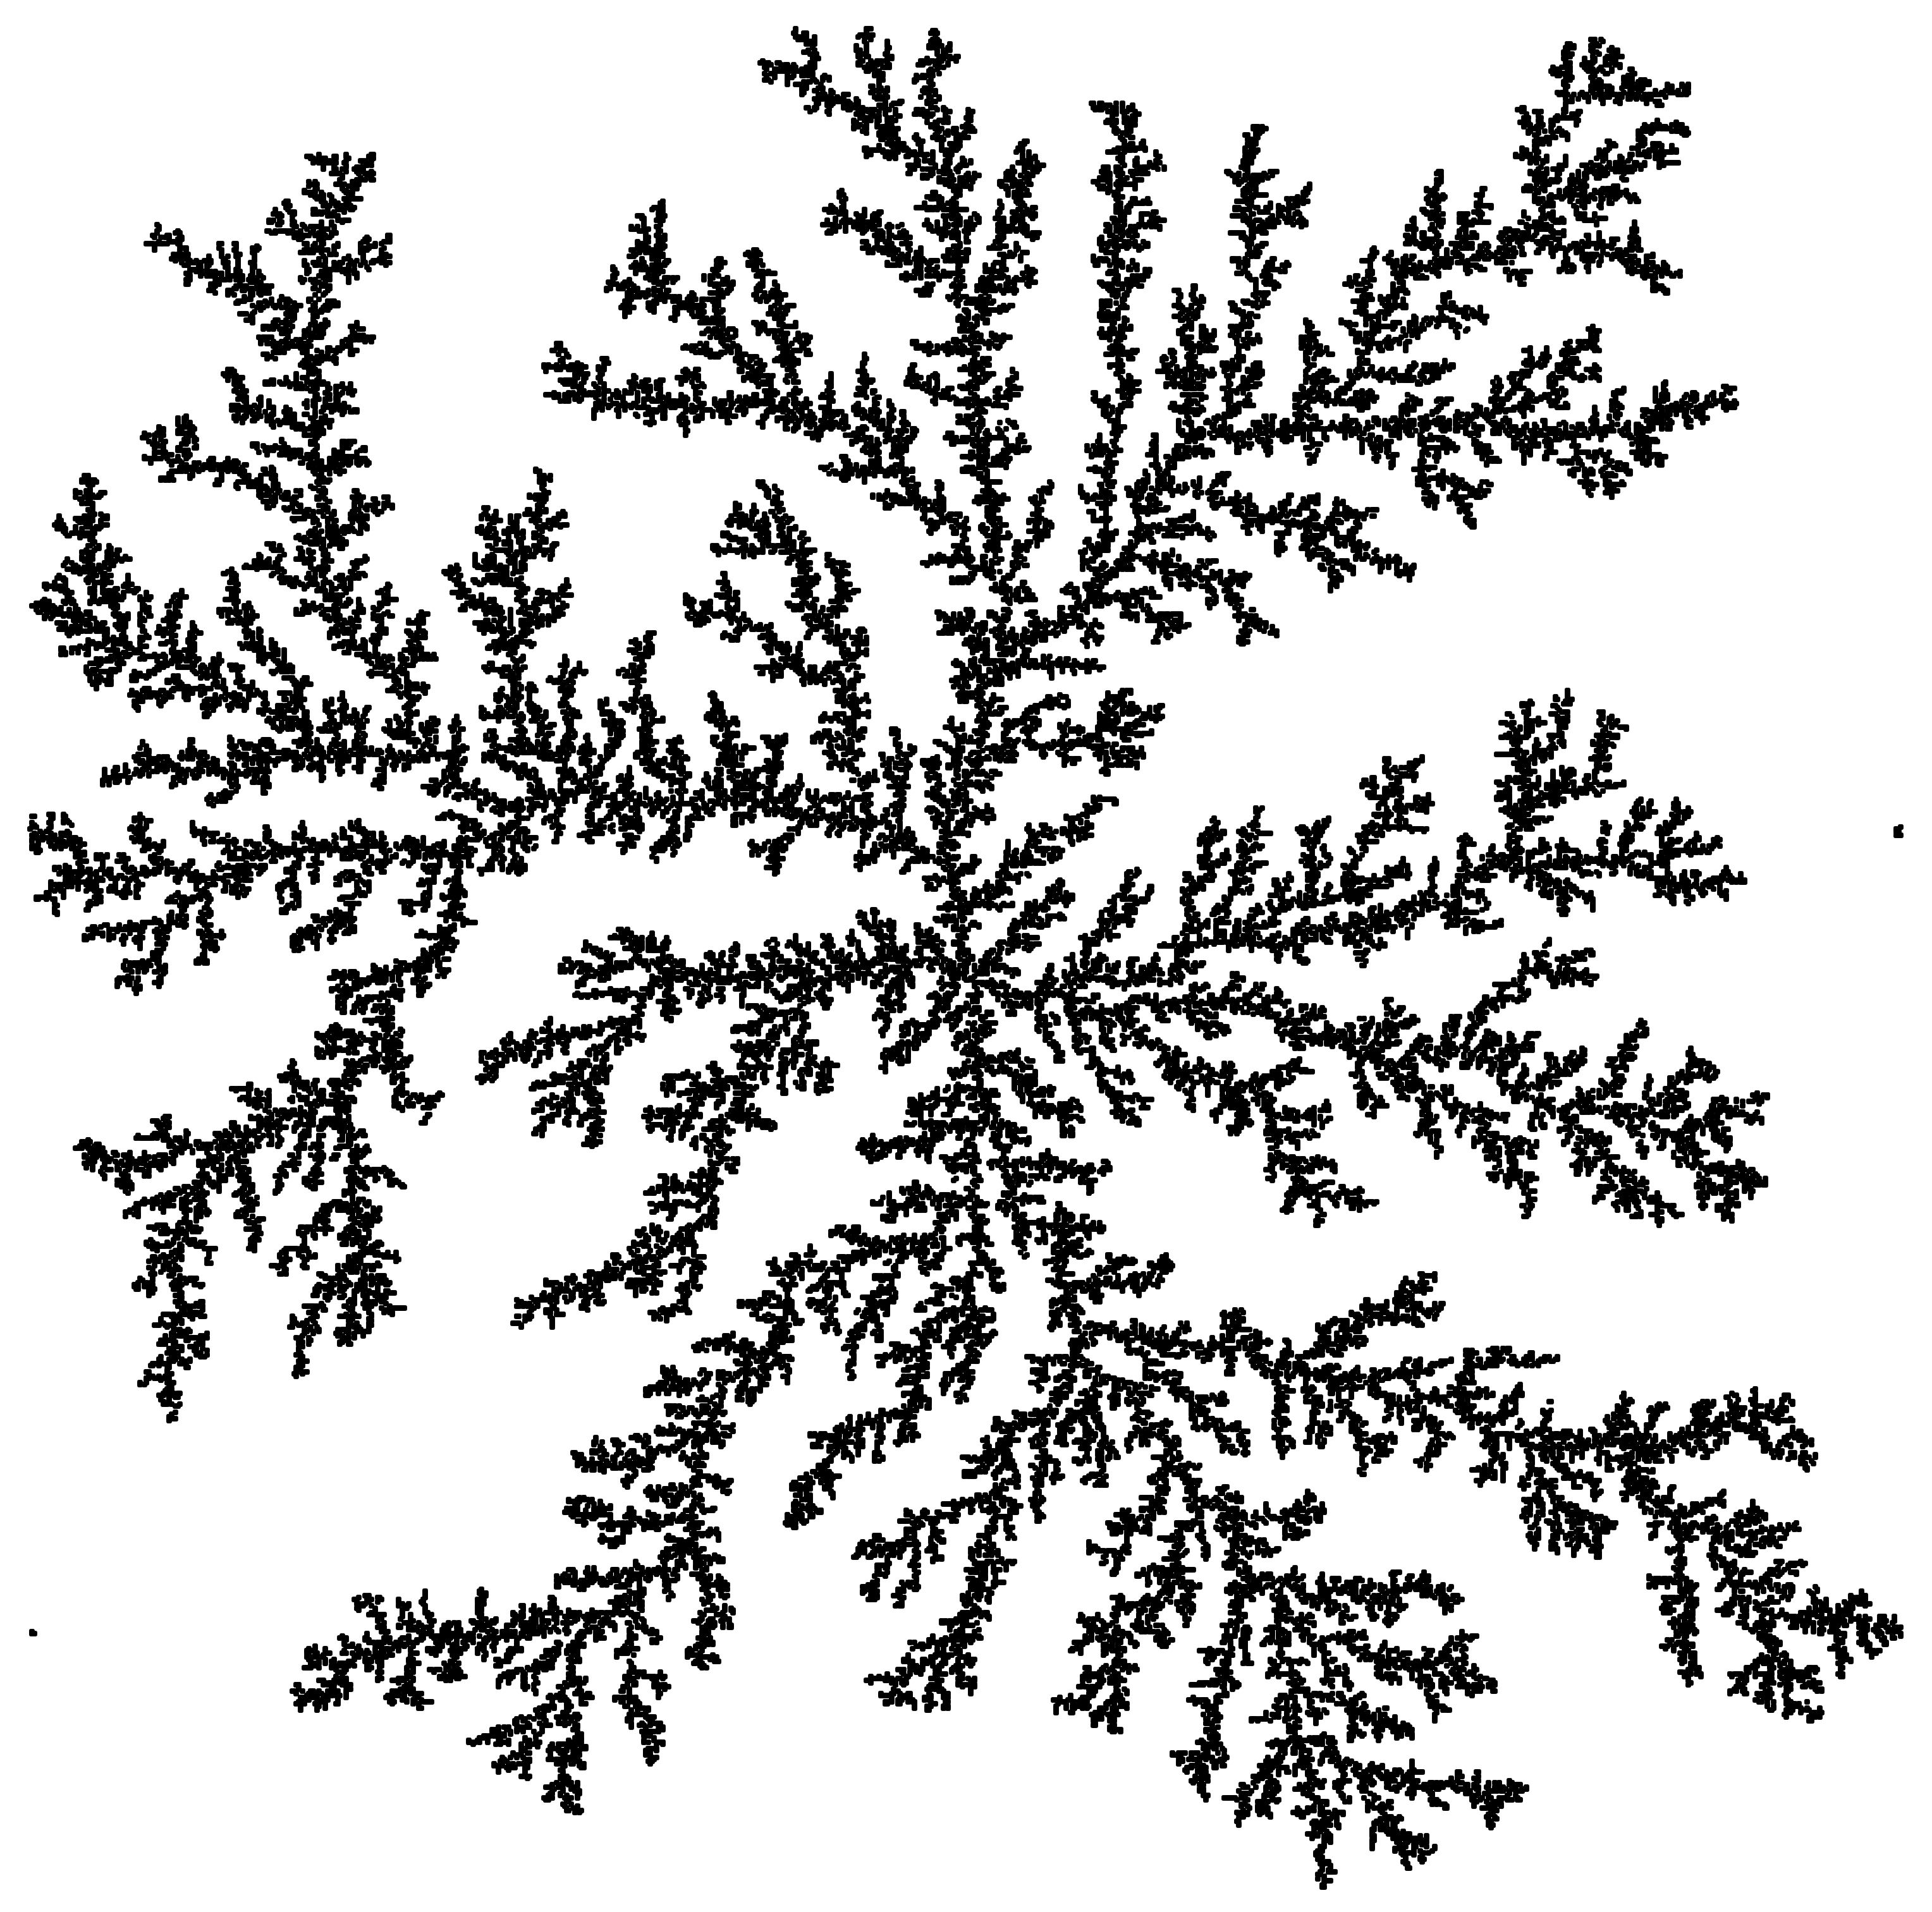
\includegraphics[width=0.43\textwidth]{nds_1_resized.png}}
        \subfloat[$nds = 200$]{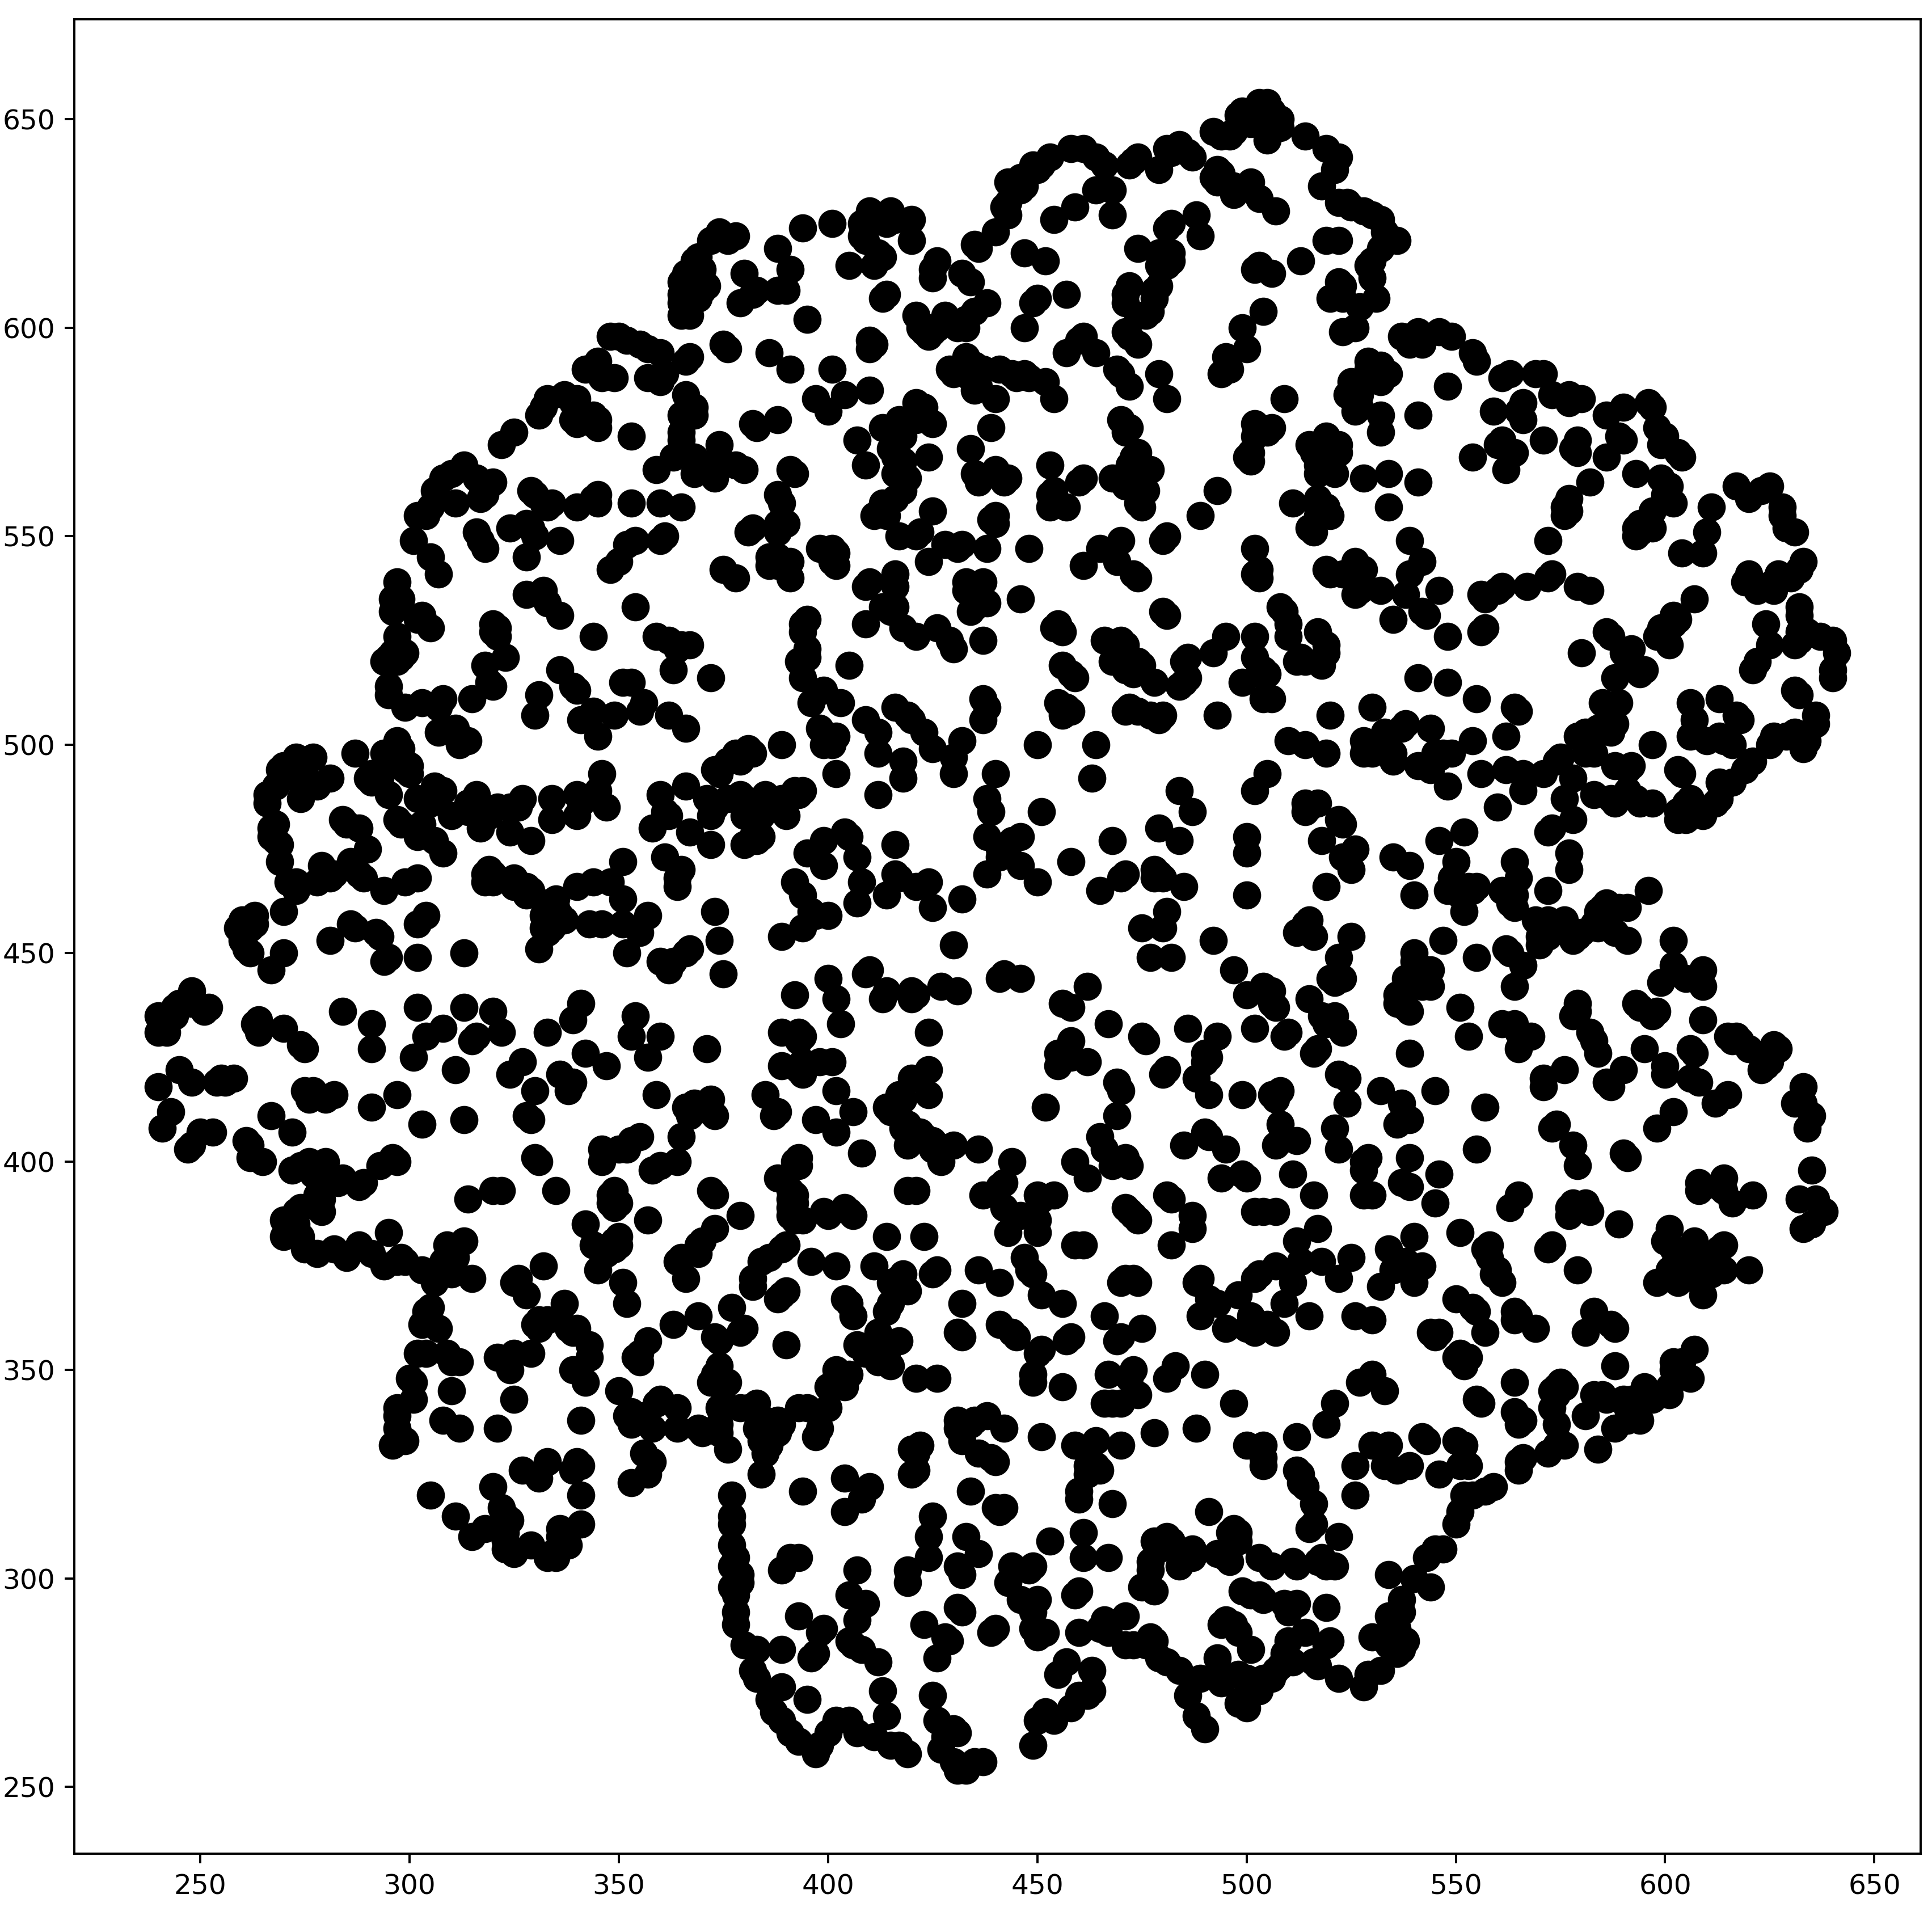
\includegraphics[width=0.43\textwidth]{nds_200_resized.png}}
    \caption{Форма на агрегата за 900x900 A2A CA при начална концентрация на дифундиращи частици c = 10\%.}
    \label{fig:nds_effect}
\end{figure}

\autoref{fig:nds_effect} демонстрира директно влиянието на различния брой стъпки на обновяване на дифузионното поле - при малки стойности на $nds$ имаме познатия от DLA агрегат, подобен на \autoref{fig:brownian_tree}, а при големи - получаваме значително по-компактна структура, с граница много по-близо до кръг. Допълнително, и за двата агрегата от крайната им структура не можем да разпознаем симетрията на решетката върху която са раснали (квадратна), т.е. в една по-разширена версия на такъв клетъчен автомат, в която са моделирани и кинк позициите бихме искали да получим и този ефект на възпроизвеждане на пространствената симетрия на система в крайната структура. За настоящата цел на валидиране на $\aDg$, А2А CA все пак е достатъчно подробен модел.

Протоколът на числения експеримент ще бъде следния: Фиксираме размера на решетката на 900x900 и изследваме \textit{c = 0.025, 0.040, 0.055, 0.070, 0.085, 0.100, 0.115, 0.130} и \textit{nds = 1, 2, 4, 6, 8, 10, 25, 50, 100, 150, 200}. За всяка комбинация $(c, nds)$ правим по 4 старта (4 различни агрегата) на A2A CA. Общо, това са $8 \times 11 \times 4  = 352$ набора данни за степента на трансформация $(t^i, \alpha^i)$. За да намалим количеството данни, които трябва да обработваме, за дадена комбинация $(c, nds)$ ще усредим $\alpha - t$ кривите по агрегатите.

Тъй като тук предпоставката е за дифузионен контрол, фиксираме $g = 1$. При изследване на $D$, което получаваме от оптимизационната процедура резултатите са $D \in [1.67, 2.2]$. По тази причина отново ще фиксираме $D = 2, g = 1$, за да работим директно с $\alpha_{21}$. Ще изследваме подробно как скалата $\tau_{21}$ зависи от $nds$ и още повече - как скейлинговата експонента $\kappa$ от $\tau_{21} \propto nds^\kappa$ зависи от концентрацията $c$.

За да можем да получим експонентата $\kappa$ ще разгледаме в $\log-\log$ зависимостта на $\tau_{21}$ от $nds$.
\begin{figure}[hbpt]
    \centering
    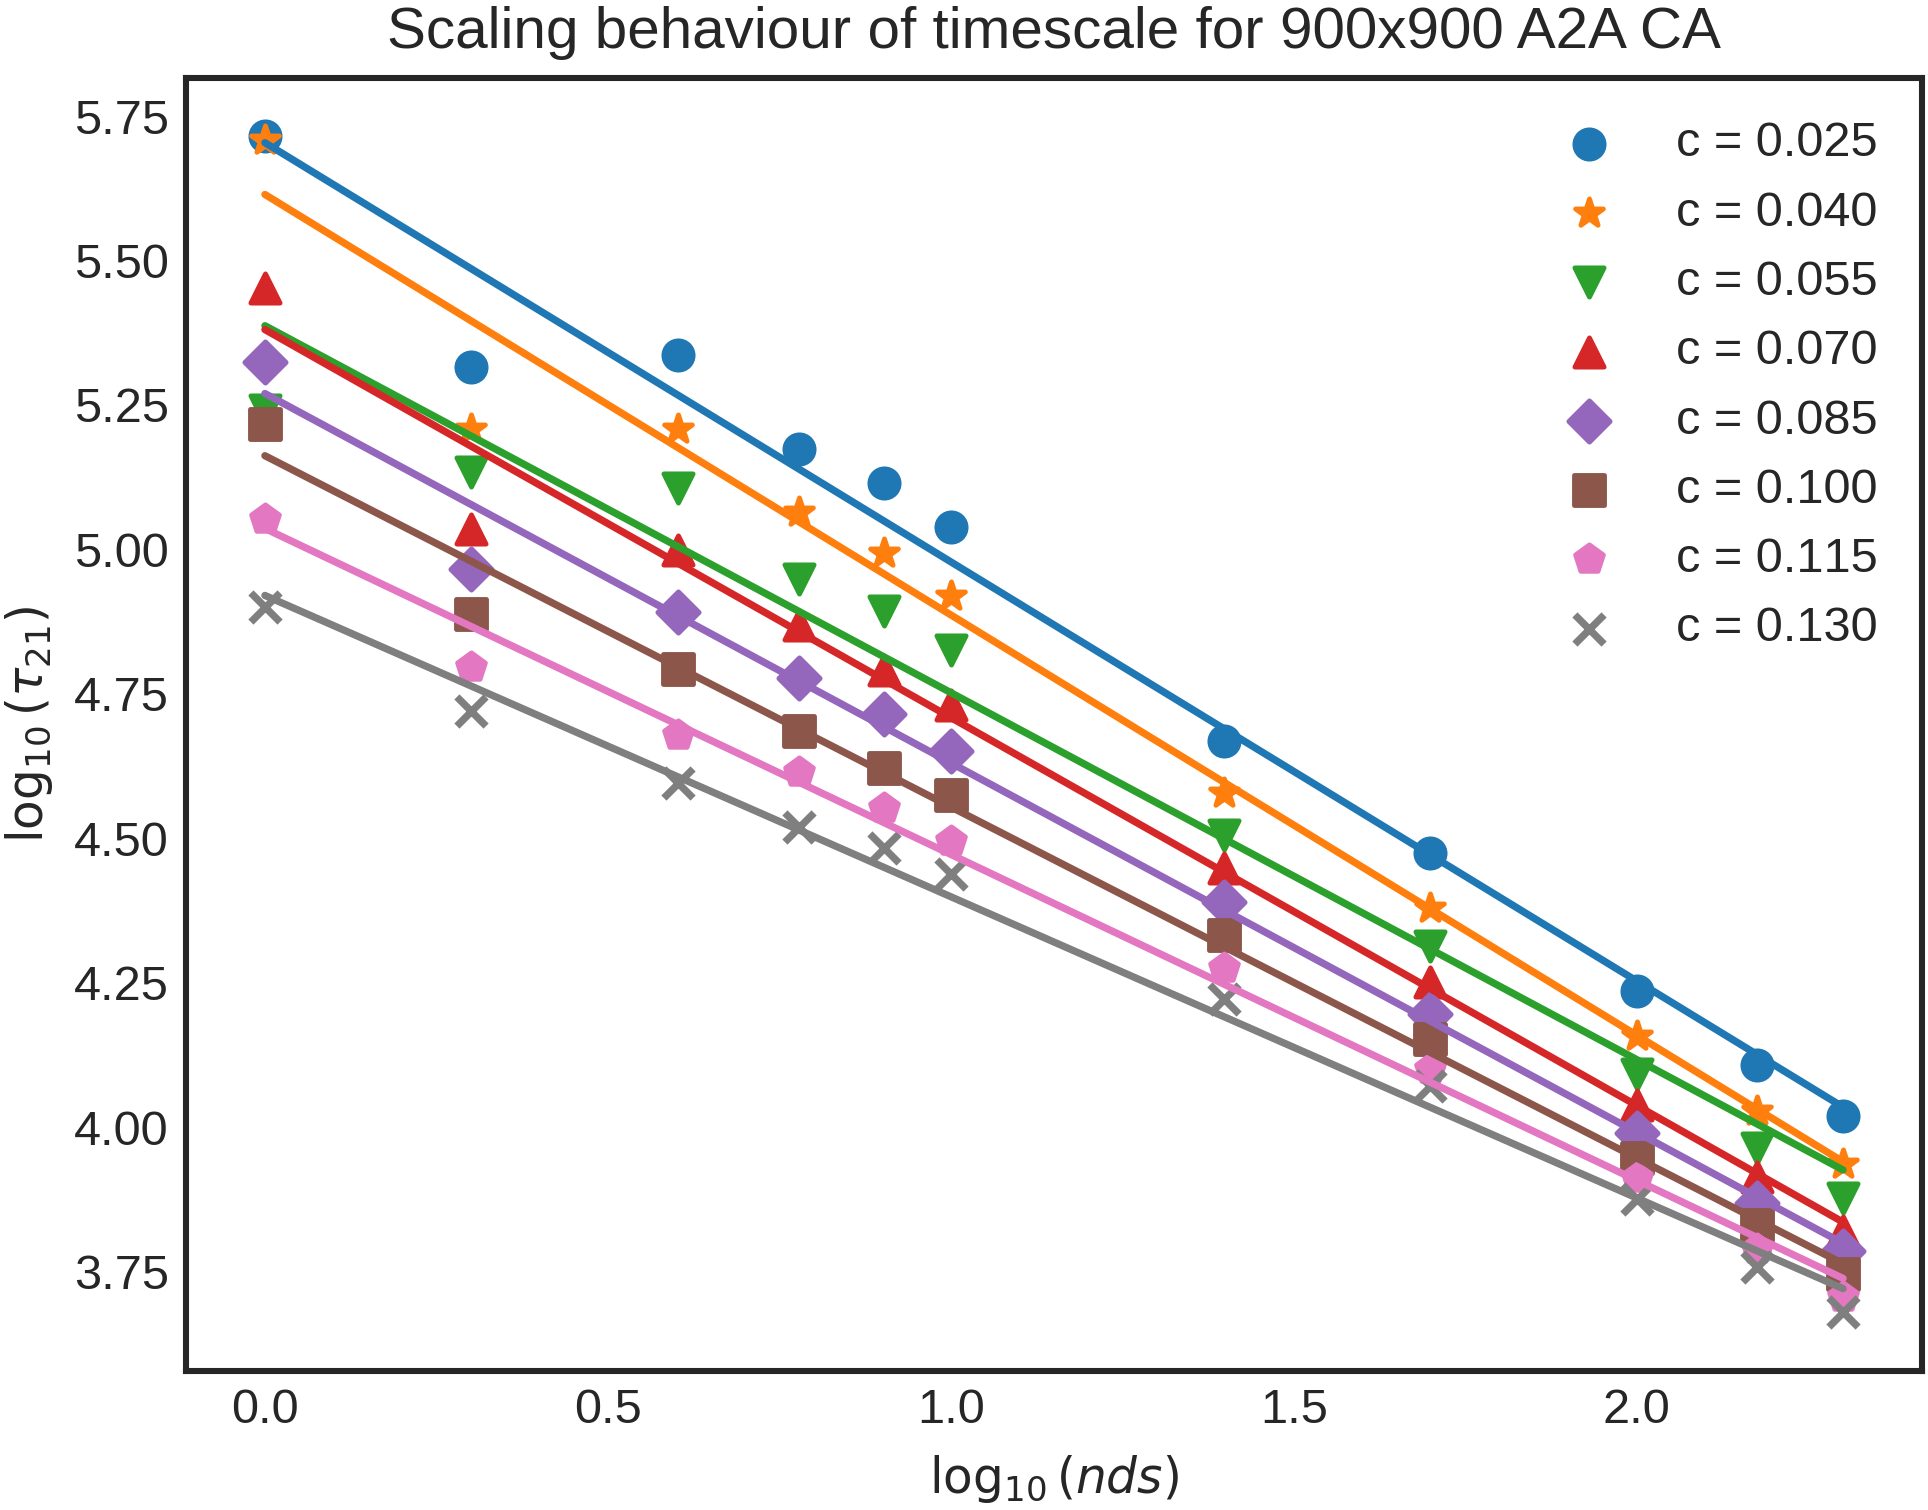
\includegraphics[width=0.85\textwidth]{scaling_plot_all_a2a_ca.png}
    \caption{Скейлинг на $\tau_{21}$ с $nds$}
    \label{fig:scaling_tau21_nds}
\end{figure}
\begin{table}[hbpt]
\centering
\caption{Резултати от линейната регресия за всяка от концентрациите на автомата.}
\label{tabl:scaling_tau21_nds}
\resizebox{0.65\textwidth}{!}{%
\begin{tabular}{@{}cccc@{}}
\toprule
Концентрация ($c$) & Наклон $(\kappa)$    & Отрез    & $R^2$    \\ \midrule
0.025        & -0.725204 & 5.703861 & 0.986310 \\
0.040        & -0.727381 & 5.614268 & 0.985010 \\
0.055        & -0.634860 & 5.387181 & 0.977654 \\
0.070        & -0.671192 & 5.380443 & 0.989942 \\
0.085        & -0.639080 & 5.269890 & 0.993133 \\
0.100        & -0.607593 & 5.162227 & 0.994085 \\
0.115        & -0.563946 & 5.036357 & 0.994955 \\
0.130        & -0.521279 & 4.920473 & 0.993984 \\ \bottomrule
\end{tabular}%
}
\end{table}

\autoref{fig:scaling_tau21_nds} и \autoref{tabl:scaling_tau21_nds} потвърждават очакванията за температурната зависимост на $\tau_{21}$ - с увеличаване на температурата процесът на агрегация (кристализация) се ускорява и съответно характеристичното му време намалява.

Наклонът на регресионните прави от \autoref{tabl:scaling_tau21_nds} е експонентата $\kappa$, докато отрезът е характеристичното време при $nds = 1$. Намаляването на $\tau$ с $nds$ е относително ,,бавно`` - два порядъка промяна по $nds$ водят до по-малко от два порядъка намаляване на характеристично време за всяка от концентрациите.

\begin{figure}[H]
    \centering
    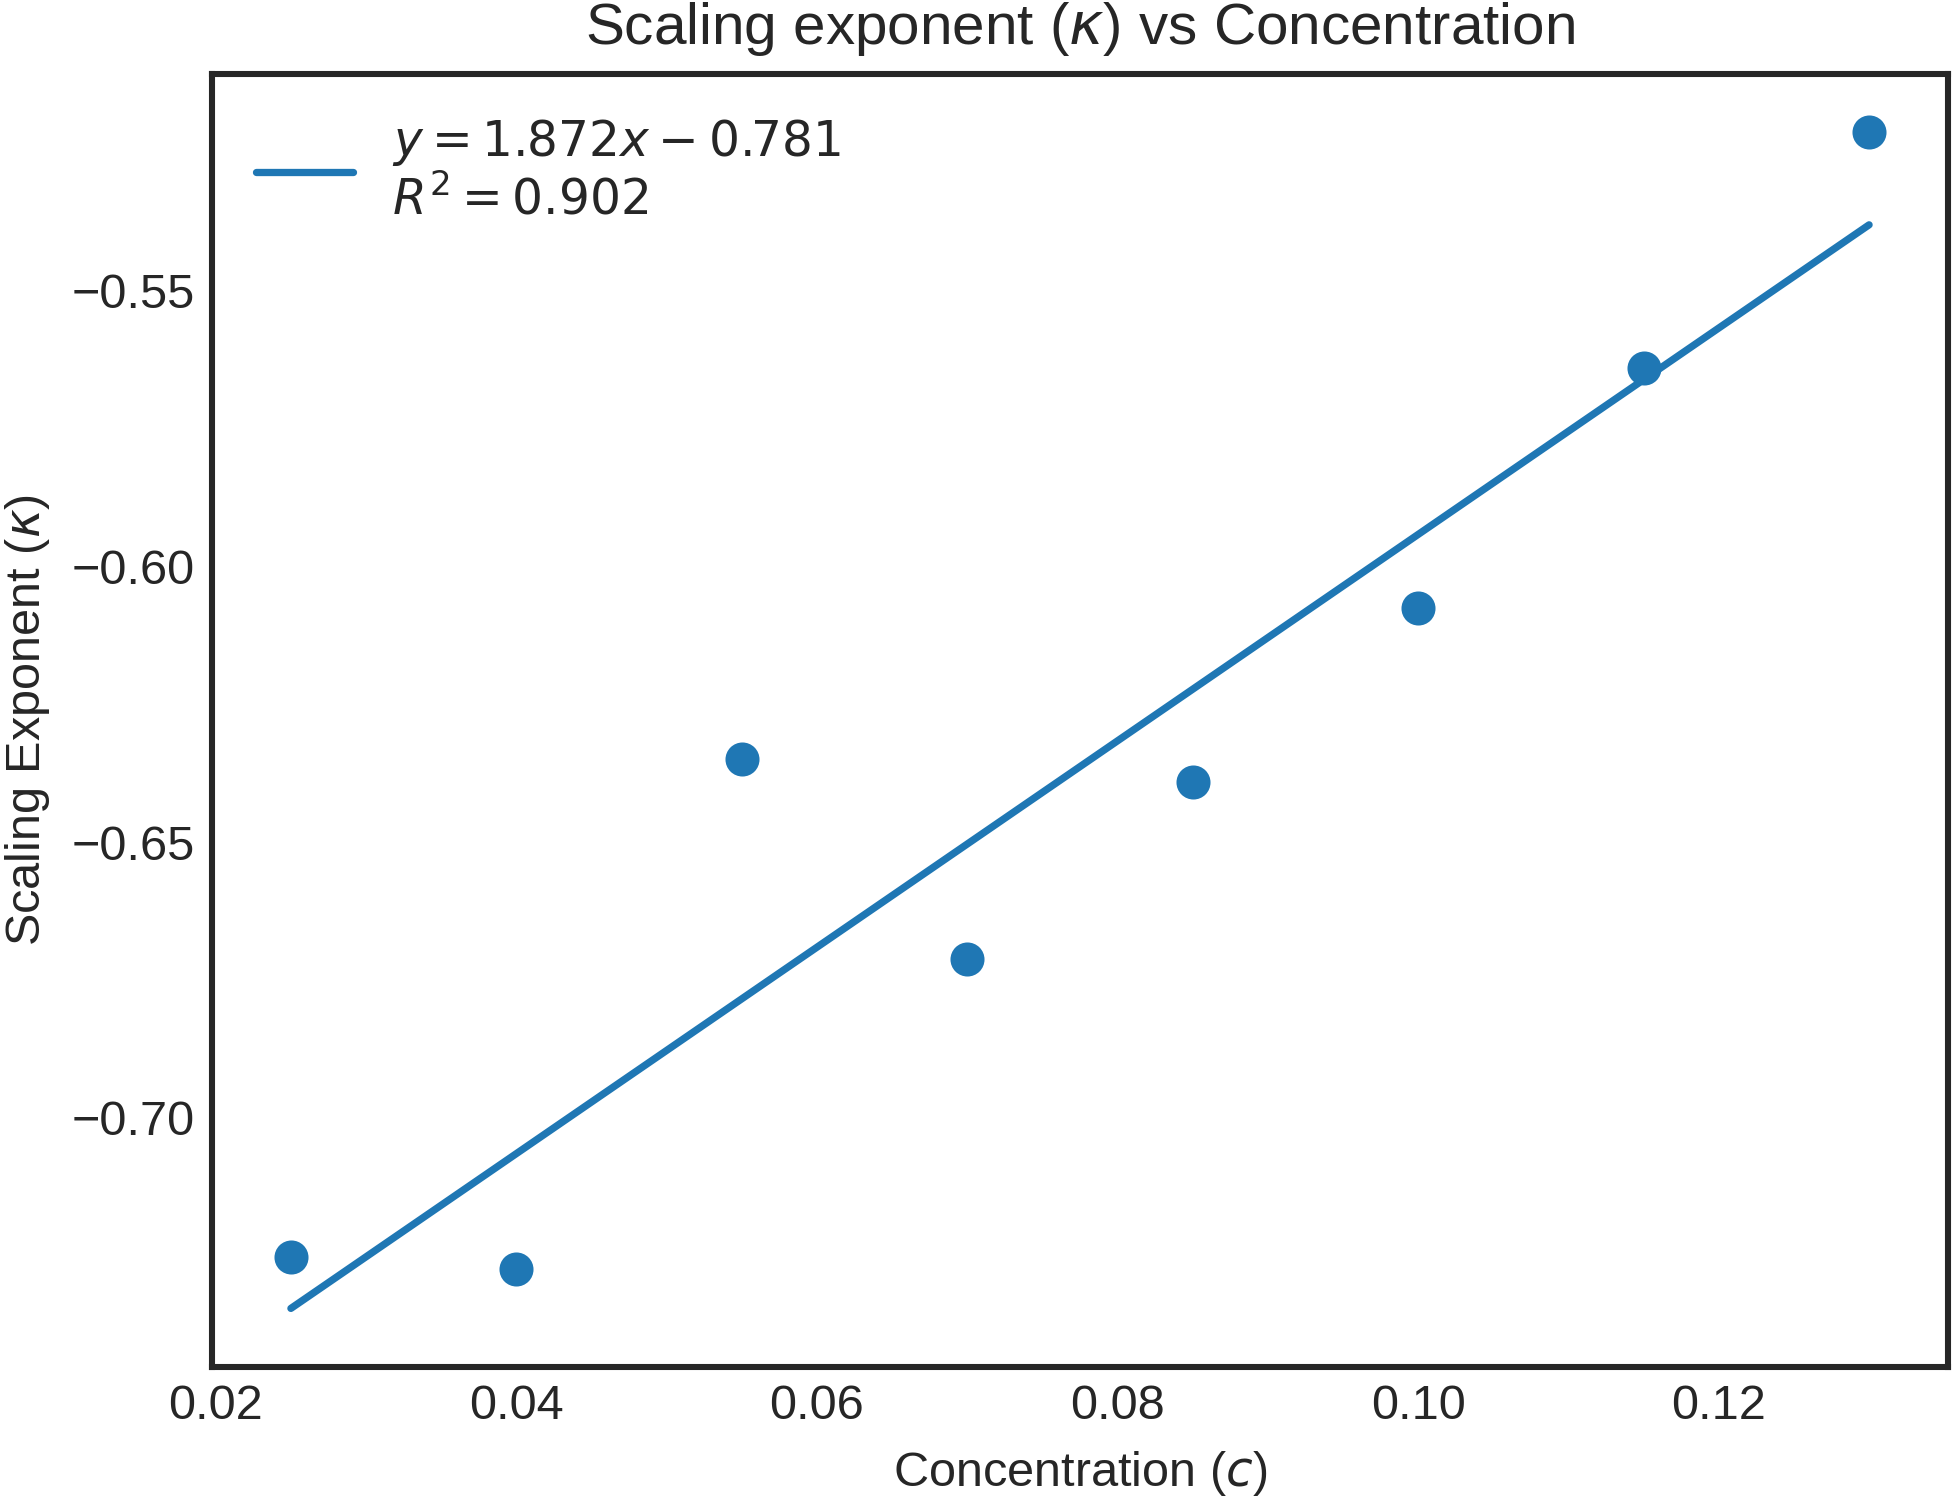
\includegraphics[width=0.7\textwidth]{slope_vs_conc.png}
    \caption{Зависимост на експонентата $\kappa$ от концентрацията $c$}
    \label{fig:scaling_kappa_vs_conc_ca}
\end{figure}

В \autoref{tabl:scaling_tau21_nds} има генерална тенденция $\kappa$ да нараства с концентрацията. За целта на \autoref{fig:scaling_kappa_vs_conc_ca} е изследвана именно тази зависимост. Тук линейната зависимост не е толкова недвусмислена, както при \autoref{fig:scaling_tau21_nds},но въпреки това очертава общата тенденция на нарастване на $\kappa$ в този интервал от концентрации, както и поставя въпроса (при екстраполация) как би изглеждала граничната стойност на $\kappa^0 = \kappa (c \rightarrow 0)$. Тъй като $\kappa ^ 0$ би било трудно да се оправдае физически (при липса на частици - не се образува агрегат), би следвало преди да си позволим такива разсъждения да изследваме поведението на все ,,по-разреден`` A2A CA.

\subsection{Обобщение на резултатите за модела} 
От валидиране с данните на \textit{Min, Sinclair, et. al.} \cite{Min2005} беше показана силата на $\aDg$ модела да описва експерименти, които JMAKn не може да обясни. Показано беше, че точките с най-голяма дискриминативна сила за двата модела са тези при големи степени на превръщане ($\alpha \rightarrow 1$), близки до равновесието. Това противоречи на пряката интуиция, защото бихме очаквали близо до равновесието всички разлики в режима на растеж да са ,,изгладени`` и детайлите на механизма да са ,,загубени``, а точно тези части на процеса се оказват най-характеристични. От експерименталните данни в предния параграф видяхме, че завиването надясно в Аврами координати е физически важно.

Валидирането с данните от симулация на A2A CA поставят $\aDg$ модела като добър инструмент за изследване на температурната зависимост на различни системи на агрегация и кристализация. A2A CA ни позволяват да генерираме много повече данни, с които да изследваме поведението на модела и моделните системи, отколкото би било практически постижимо при изследване на такива реални системи.

Можем да дадем следната ,,рецепта``, която да се прилага за $\aDg$:
Единият подход е да използваме директно числените процедури от \autoref{subsub:parametric_identification} и ако получените параметри са близки до цели числа, ги закръгляваме до съответното най-близко цяло, избираме съответната аналитична крива и правим параметрична идентификация за времевата скала. Ако получените параметри са извън $ 0.5 \le D \le 3.5$ и $0.5 \le g \le 2.5$ считаме, че данните не могат да бъдат обяснени с модела. 

Аналогично, когато сме сигурни, че имаме режим на дифузионен контрол, т.е. $g = 1$, можем да направим параметрична идентификация за $n$, $\tau$ от JMAKn, тъй като там имаме общ аналитичен израз. От уравнението на \autoref{fig:nvsd_graph} за полученото $n$ избираме $D$ и го закръгляваме. Нататък повтаряме предната процедура.

Ако при всеки от двата подхода за избраната $\aDg$-крива коефициентът на Пиърсън $R^2$ е малък, също считаме че моделът не може да обясни добре наблюдавания експеримент.

Тези ограничения върху целите стойности може да изглеждат ненужни и твърде строги, особено с процедурите от \autoref{subsub:parametric_identification}. Ние обаче ги налагаме така щото да държим сметка за началните предположения, при които е изведен модела, за да може те да имат ясен физичен смисъл. 
С използването на модела и задълбочаването на познаването му в контекста на различни експериментални данни, можем да си позволим да освободим размерността да бъде реално число, т.е. да твърдим че $D$ e фракталната размерност на растящия кристал. Такава ретроактивна промяна на смисъла на един параметър трябва да бъде направена внимателно, само когато са на лице подходящи експерименти, с които тази хипотеза да бъде изследвана. Такъв числен експеримент би бил например клетъчен автомат, растящ послойно от 2D към 3D. Ако получаващите се стойности от \textit{NLSQ/Uniform} корелират с фракталната размерност на автомата, то бихме могли да направим такава рационализация за $D$.
\section{Йерархия на сигмодините модели}
\subsection{Експериментът на Марков и Стойчева}
Тук ще прехвърлим фокуса от получаването на конкретен модел към изграждане на кратка йерархия на база поведение, брой параметри, физичен смисъл на параметрите и т.н. Експерименталните данни, спрямо които ще сравняваме моделите са тези на \textit{Марков и Стойчева} от 1976~г. \cite{Markov1976}. Това са едни от най-фините експерименти за зародишообразуване под действието на външен електричен потенциал.

В този експеримент е изследван броят на зародишите като функция на времето и  концентрацията на електролит при електроотлагане на $Hg$ от воден разтвор на $Hg_2(NO_3)_2$ върху ,,безсктруктурен`` \textit{планарен} $Pt$-електрод. В статията си \textit{Марков и Стойчева} правят заключение, че в началото има \textit{линейно нарастване} на броя зародиши и след това се достига плато. Броят зародиши, в платото зависи от експерименталните условия. От \textit{Фиг. 5} на \textit{Марков и Стойчева}, се вижда че броят зародиши всъщност следва сигмоиден закон. Още повече, отлагането върху планарен електрод предполага \textit{квази-двумерен растеж} $(D=2)$. Тези експериментални условия ще бъдат важни за избора на модел, като най-подходящ от разглежданите.

\subsection{Модели за описание на данните}
Ще използваме по-общата дефиниция на степен на превръщане \autoref{eq:alpha_ndef_def} през $N(t)$, тъй като експериментът е именно за броя образувани зародиши. Допълнително, максималният брой зародиши $N_{max}$, ще направим параметър на модела, подлежащ на идентификация. Общо трите модела, които ще разгледаме, ще записваме във вида:

\begin{equation*}
    N(t) = N_{max} f(\overline{p}, t)
\end{equation*}
Където $f(\overline{p}, t)$ е дясната страна на интегралната сигмоидна крива за конкретния модел, $t$ - време,  $\overline{p}$ e векторът с параметрите, освен $N_{max}$.
Трите модела, които ще разгледаме са Ричардс, JMAKn и $\alpha_{21}$.
\paragraph{Ричардс.} Това е един от най-общите модели на сигмоиден растеж, с множител отчитащ положителната обратна връзка и такъв, отчитащ самоограничаването поради изчерпване на ресурс (пресищането в контекста на кристалния растеж). Той е изведен като обобщение на логистичните модели в контекста на описание на растежа на популации. Диференциалната форма на Ричардс е:
\begin{equation}
    \label{eq:richards_diff_form}
    \frac{d(N/N_{max})}{dt} = \frac{k N}{N_{max}(q-1)}\left[ 1 - \left(\frac{N}{N_{max}}\right)^{q-1} \right]
\end{equation}
В основното ОДУ се вижда, че членът отговарящ за положителната обратна връзка води до $N \propto e^t$ за малки времена. Това ОДУ може да бъде интегрирано точно, за да бъде получено решение в затворен вид \cite{Richards1959}:
\begin{equation}
    \label{eq:richards_int_form}
    N(t) = \frac{N_{max}}{\left\{1 + (q-1)\exp{\left[ - (t-t_{i})/t_k \right]}\right\}^{\frac{1}{q-1}}}
\end{equation}
Където $t_k = 1/k$, е характеристичното време на процеса, $k$ - кинетичен коефициент, $t_{i}$ е времето, в което се достига инфлексната точка. Може да се покаже \cite{Tjrve2010}, че $N_i (t_i) = N_{max} d ^ {\frac{1}{1-d}}$. И съответно времевата скала е:
\begin{equation*}
    \tau_R = t_i q ^ {\frac{1}{q-1}}
\end{equation*}
Рескалираме и получаваме безразмерната форма:
\begin{equation*}
    \alpha \equiv \frac{N(t)}{N_{max}} = \left[ 1 + (q-1) \exp{\left( -K \left( \frac{t}{\tau_R} - q ^ {\frac{1}{1-q}} \right) \right)} \right] ^ {\frac{1}{1-q}}
\end{equation*}
Така в модела остават 2 параметъра (спрямо безразмерното време $t/\tau_R$): $K \coloneqq q^{1/(q-1)} t_i / t_k$ и $q$. Тогава и позицията на инфлексната точка е на линията $\alpha = t/\tau_R$ и не зависи от избора на $q$ и $K$.
Изборът на $q = 2$ дава познатият модел на Ферхюлст, a при $q = 1$ - Гомперц (граничен преход). Заедно с времевата скала, за
$\overline{p} = (q, K, \tau_R)$. Тогава за целите на параметричната идентификация имаме \textbf{четири} параметъра, които трябва да определим.

\paragraph{JMAKn.} Ще използваме интегралната крива във вида даден от \autoref{eq:jmakn_with_time_scale}, като заместим степента на превръщане с $N$ през \autoref{eq:alpha_ndef_def}. Получаваме:
\begin{equation}
    \label{eq:jmakn_intform_n}
    N(t) = N_{max} \left\{ 1 - \exp{\left[  \left( 2 \frac{t}{\tau_{JMAK}} \right)^n \right]} \right\}
\end{equation}
Параметрите са степента $n$ (вж. \autoref{res:jmak}) и времевата $\tau_{JMAK}$. Тогава $\overline{p} = (n, \tau_{JMAK})$. Заедно с $N_{max}$ параметрите за определяне в този случай са \textbf{три}.

\paragraph{$\boldsymbol{\alpha_{21}}$.} Тъй като експерименталните условия предполагат квази-двумерен растеж, тук директно ще използваме вариацията на $\aDg$ с $D = 2$, $g = 1$. Предимствата на този модел спрямо JMAKn в близък експериментален контекст  бяха описани в \autoref{sub:experimental_validation}. Единствено остава да запишем кривата за $\alpha_{21}$ от \autoref{sub:analytic_results} като такава за $N(t)$:
\begin{equation}
    \label{eq:alpha21_intform_n}
    N(t) = N_{max} \tanh^2{\left( 2 \frac{t}{\tau_{21}} \right)}
\end{equation}
Тук $\overline{p} = (\tau_{21})$. Заедно с $N_{max}$ общият брой параметри подлежащи на определяне е \textbf{два}.

Моделите следват ясна йерархия в броя параметри, като най-много са при Ричардс и най-малко - при $\alpha_{21}$. Най-ценен ще е такъв модел, който може да даде най-добро физично описание с най-малък брой параметри. Т.е., ако $\alpha_{21}$ дава съизмерими по $R^2$ резултати на Ричардс, ние бихме предпочели $\alpha_{21}$ заради по-малкия брой параметри и заради по-ясния им смисъл в контекста на кристализация.

Тук няма да се ограничим само с определянето на скалите за всеки конкретен модел и набор данни от \textit{Фиг. 5 и 6} от \cite{Markov1976}, a ще разгледаме зависимостта параметрите на модела и най-вече времевите скали от свръхпотенциала, при който е проведена кристализацията (еквивалент на пресищане).

\subsection{Резултати от определянето на параметрите}
\subsubsection{Ричардс}
\begin{figure}[hbpt]
    \centering
    \caption{Рескалирани данни с параметрите получени за модела на Ричардс.}
        \subfloat[Фиг. 5]{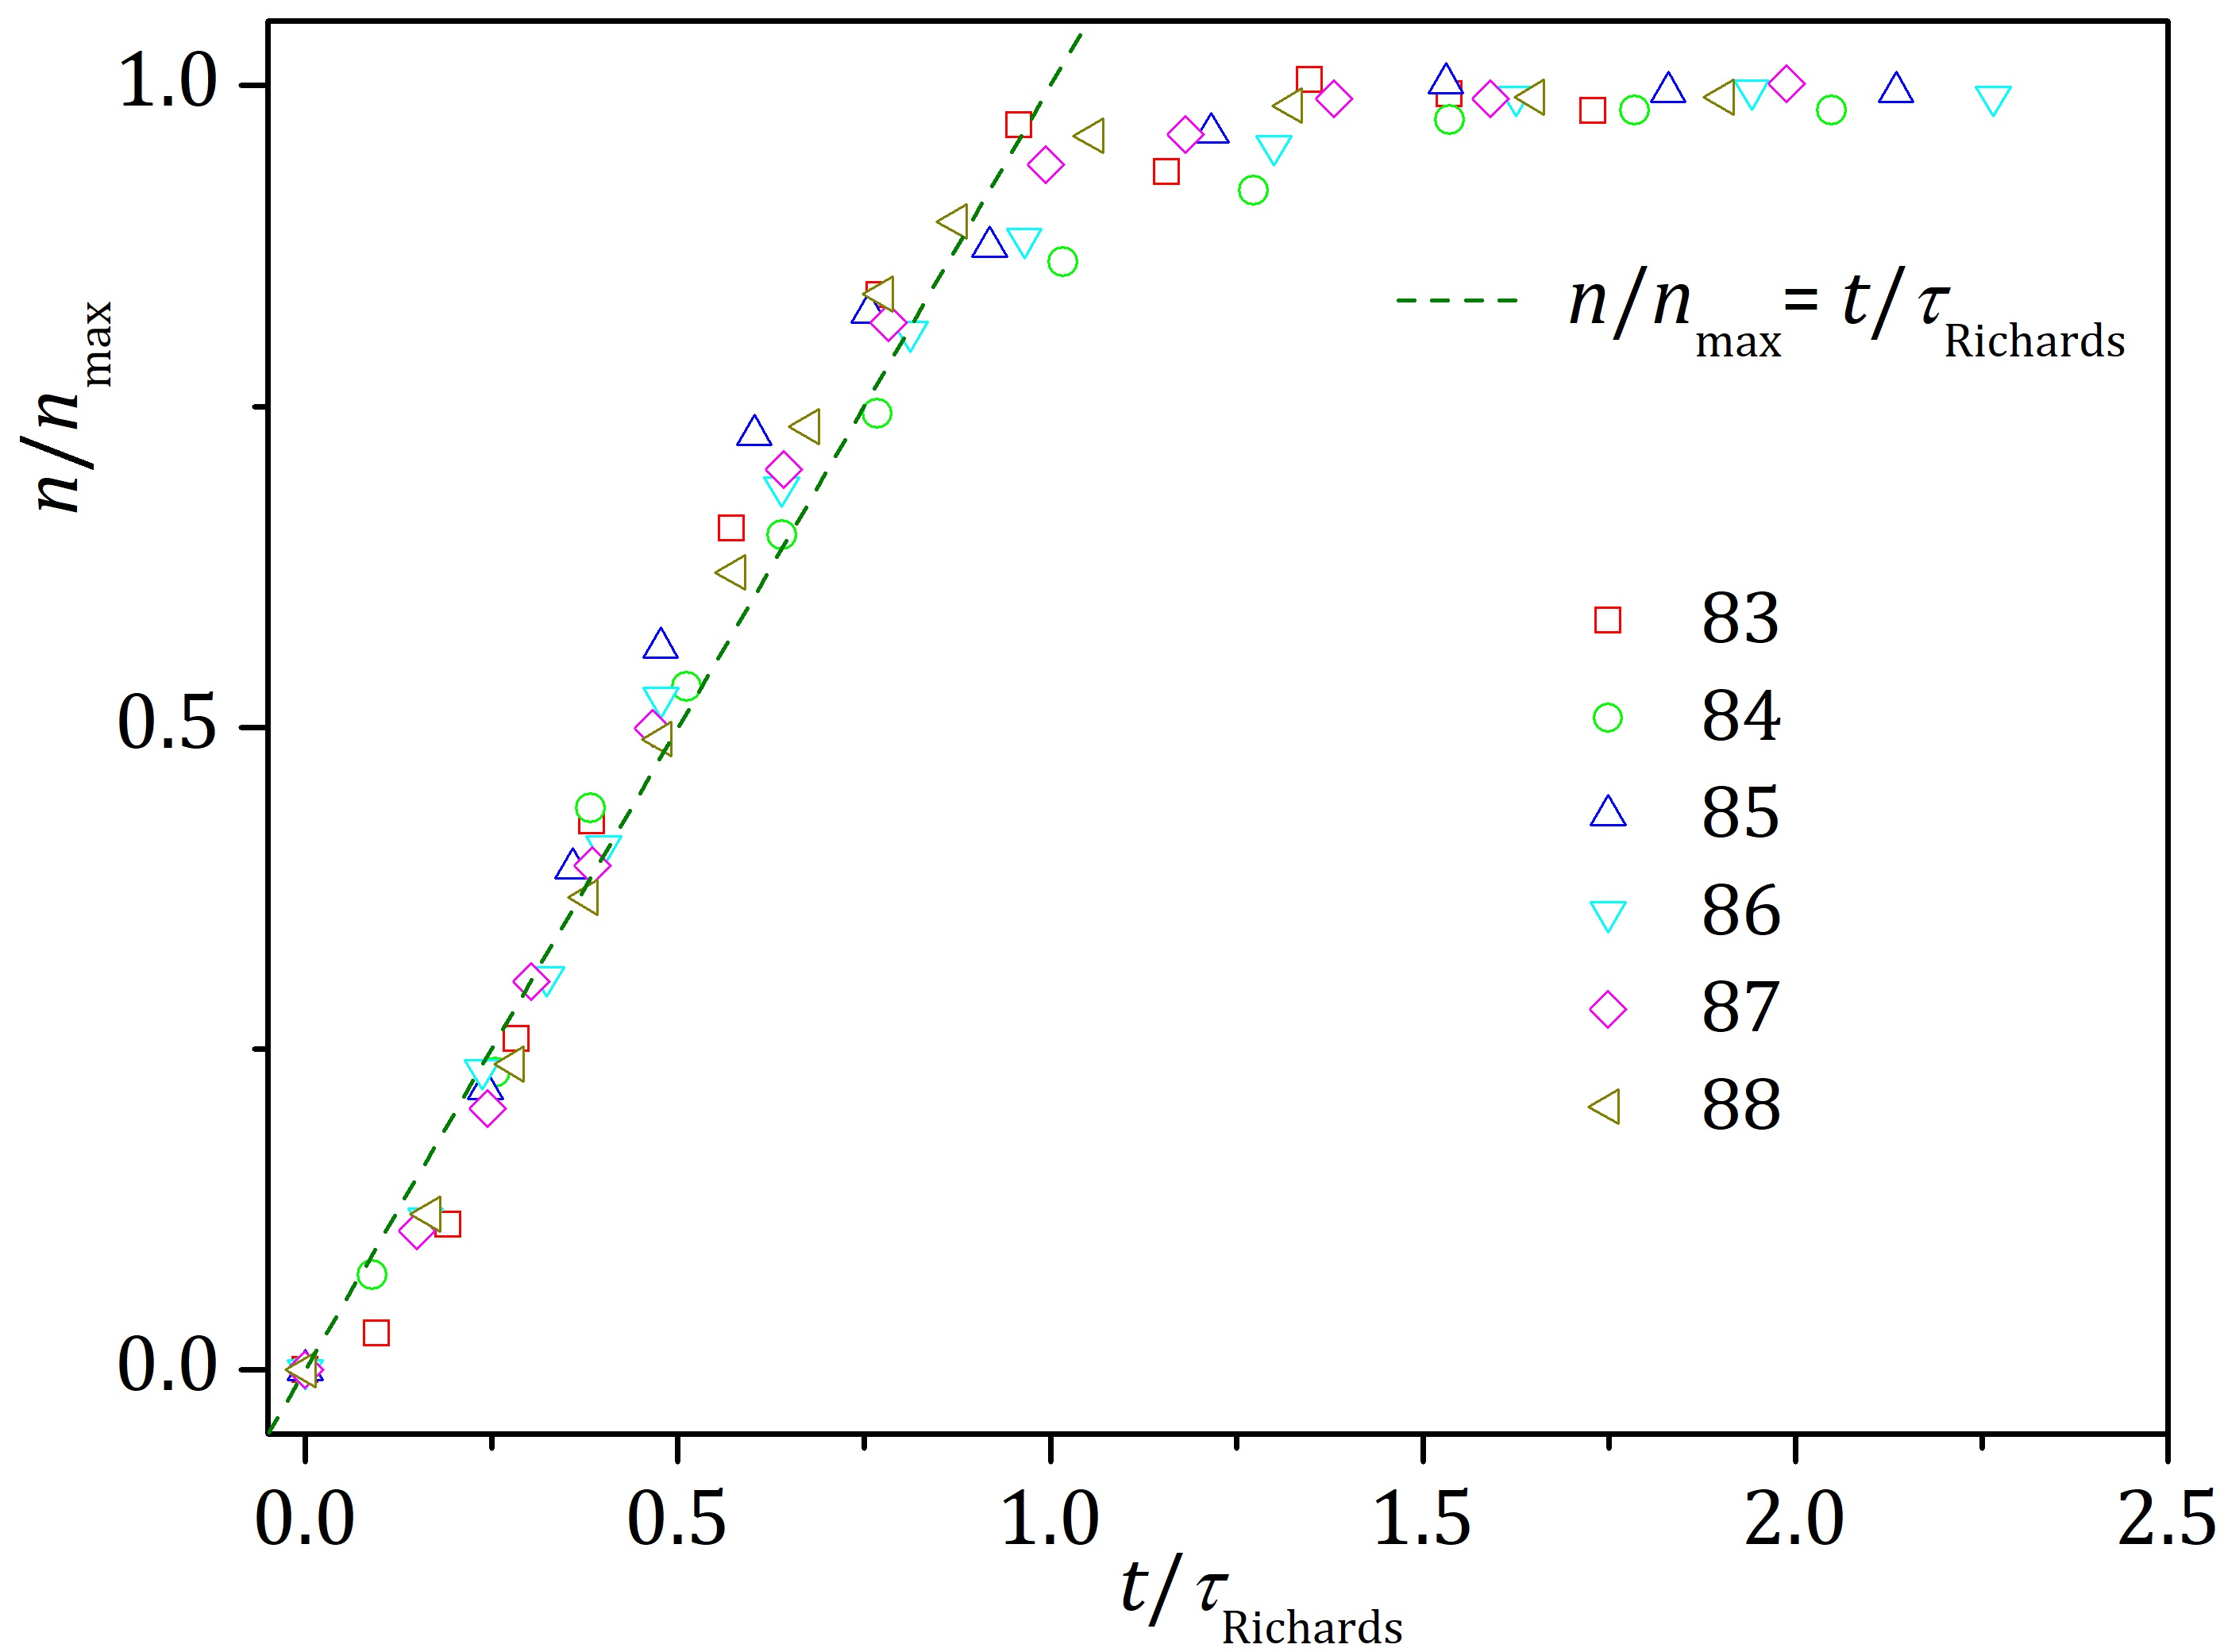
\includegraphics[width=0.43\textwidth]{ivan_markov_graphs/Fig5_Imarkov_ES_TSF1976 -Richards_rescaled.jpg}}
        \subfloat[Фиг. 6]{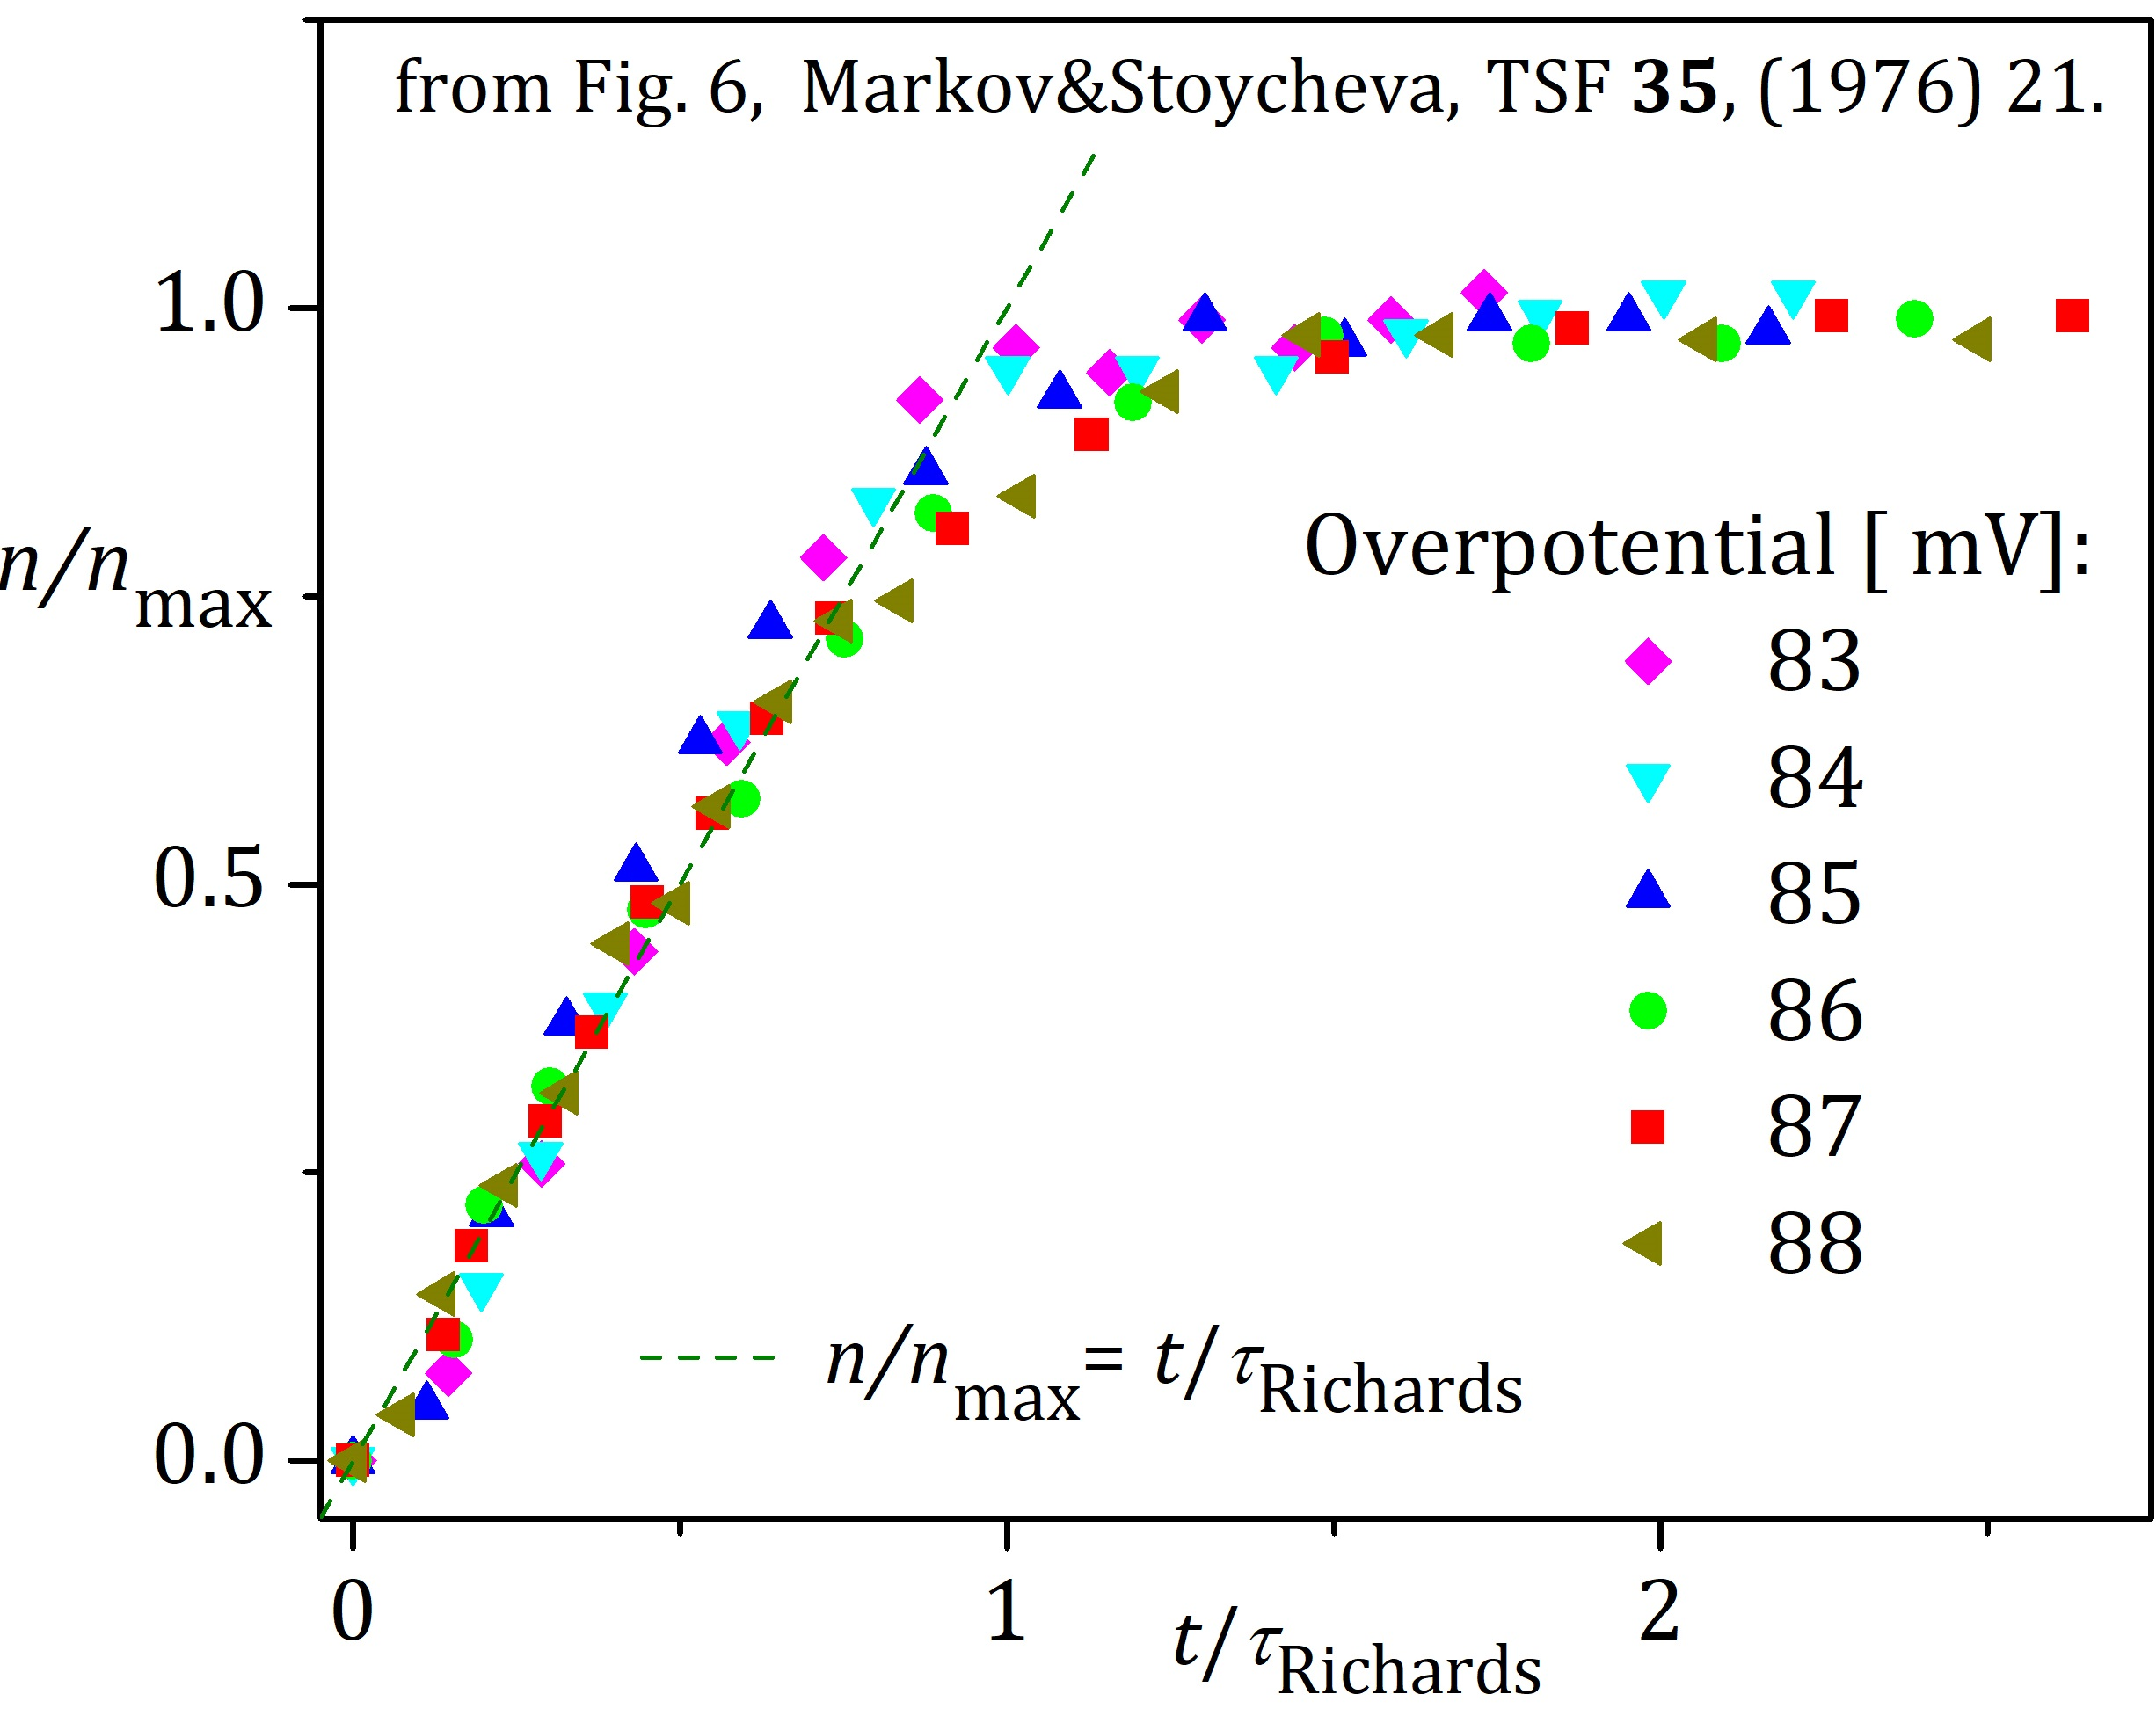
\includegraphics[width=0.43\textwidth]{ivan_markov_graphs/Fig6_Richards_rescaled.jpg}}
    \label{fig:richards_rescaled}
\end{figure}
\begin{figure}[H]
    \centering
        \subfloat[Фиг. 5]{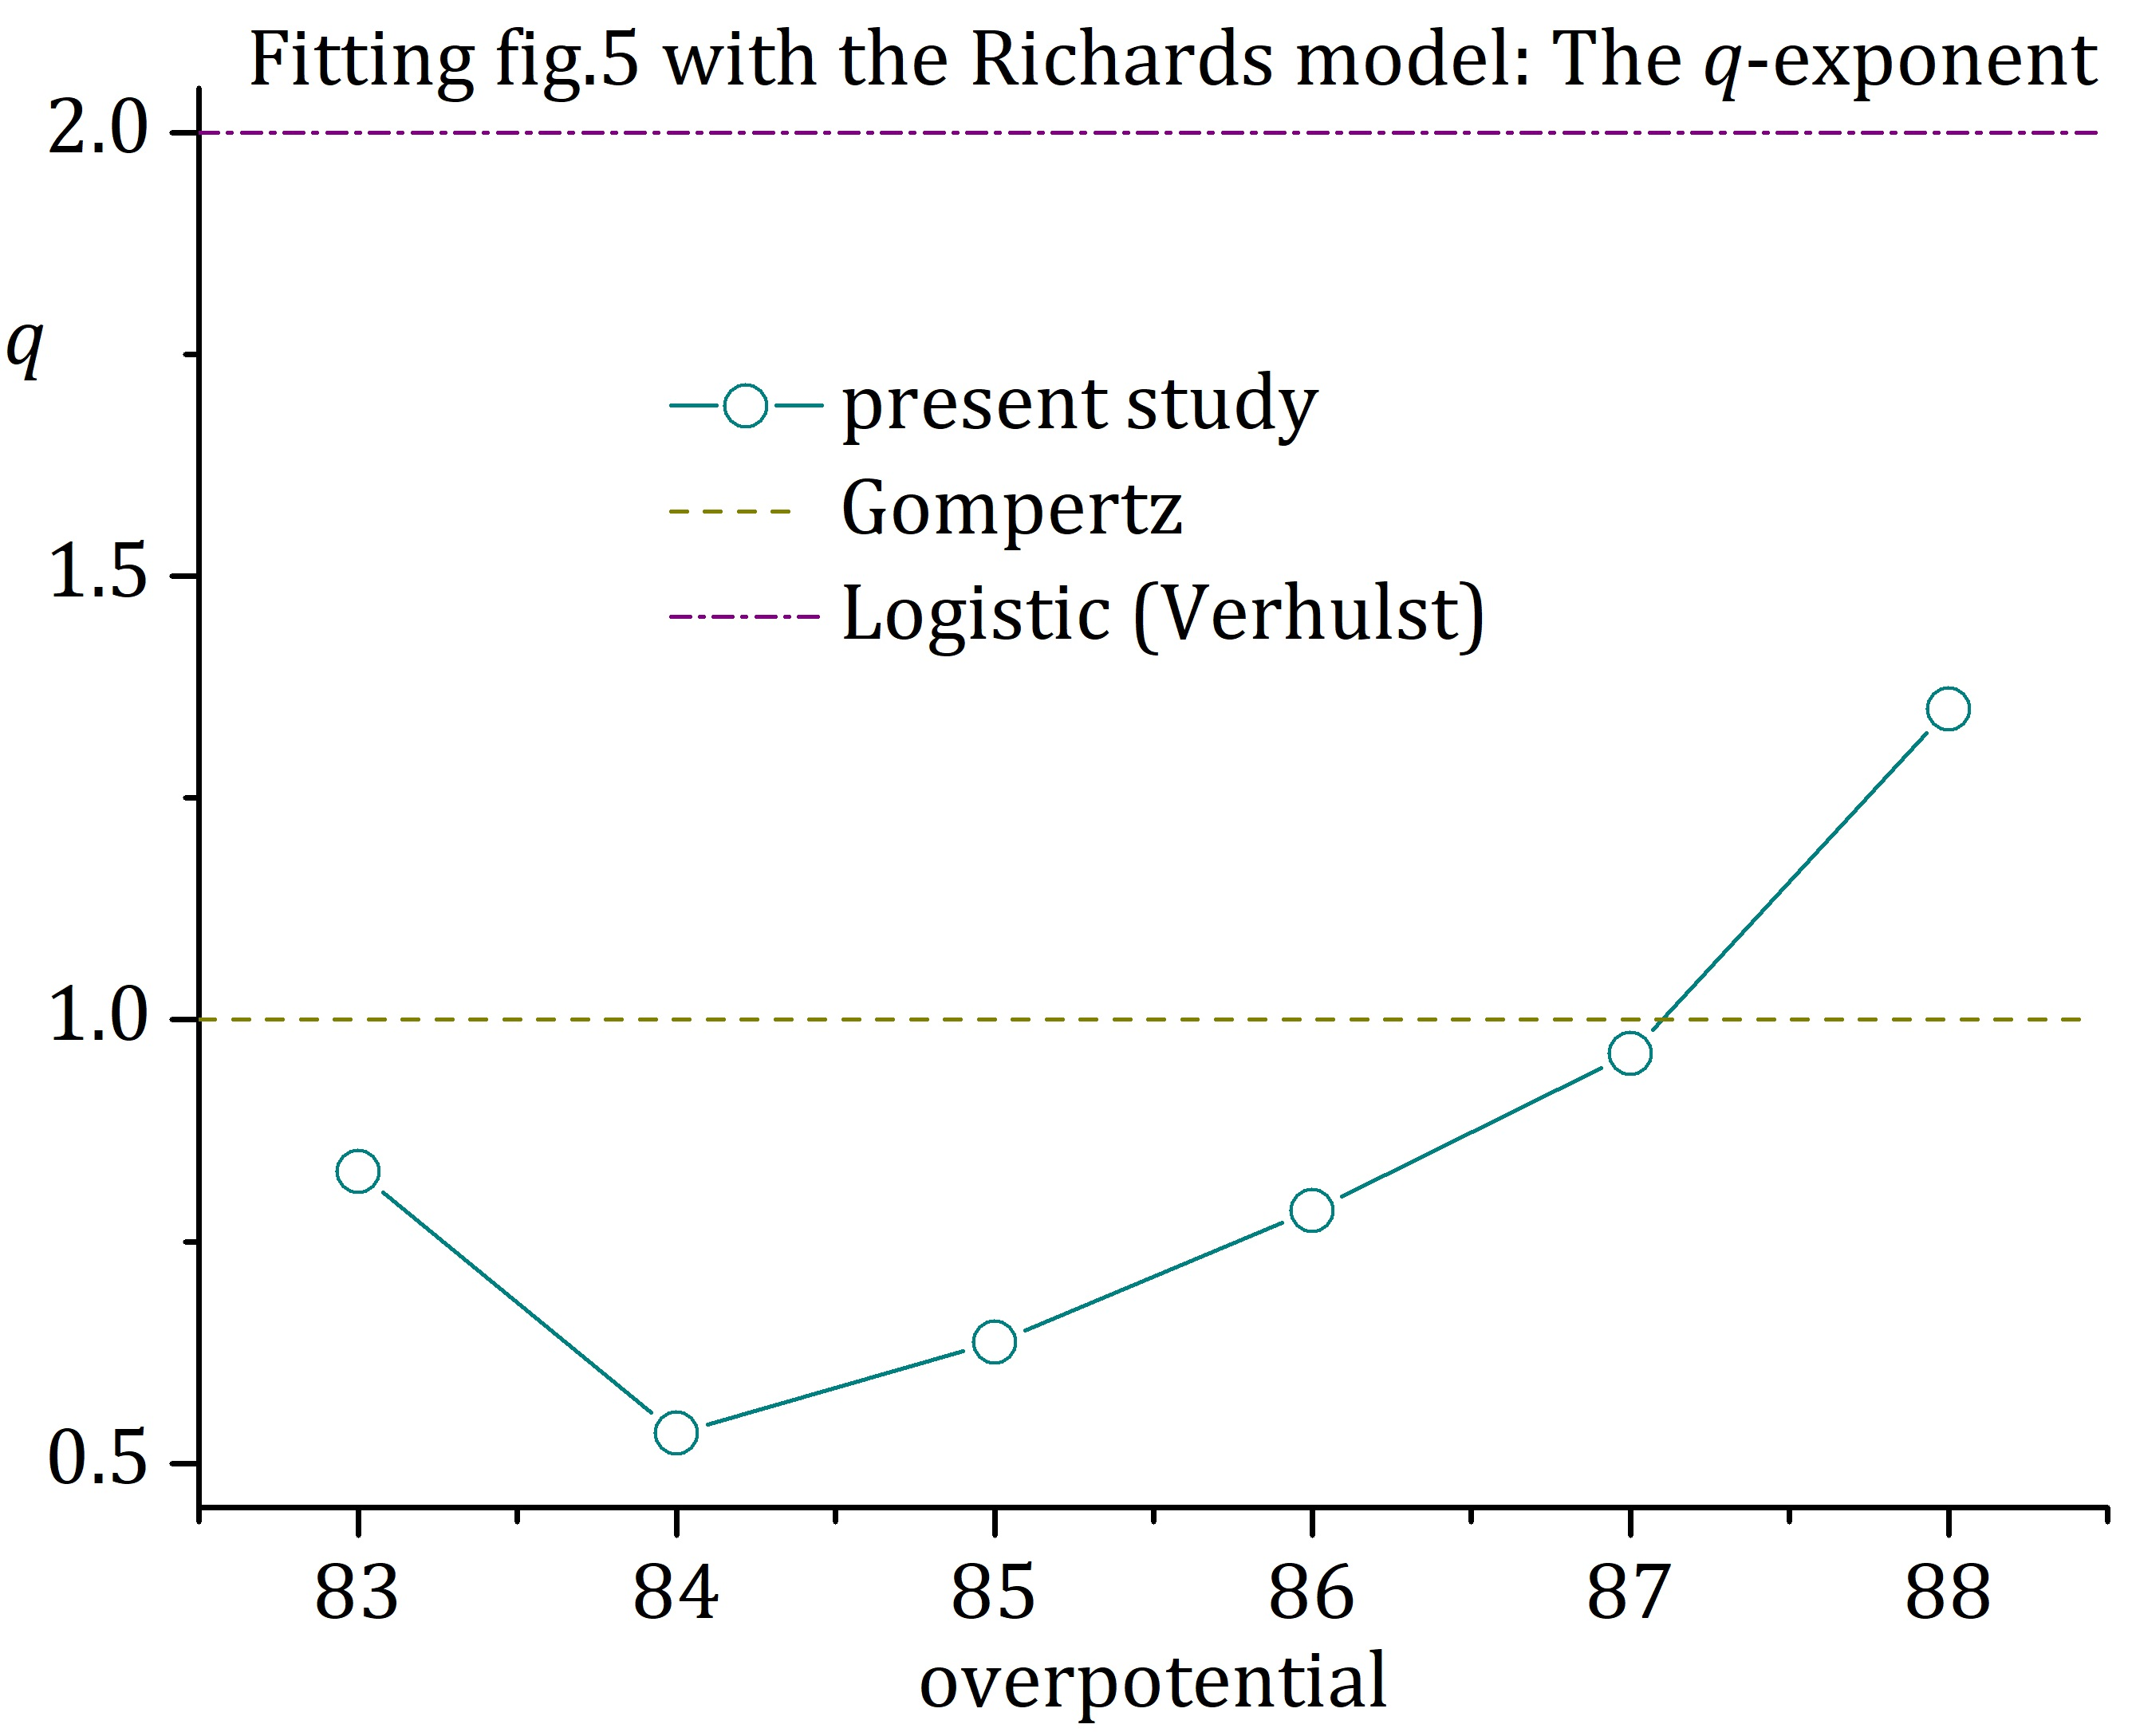
\includegraphics[width=0.40\textwidth]{ivan_markov_graphs/Fig5_q-overpotential.jpg}}
        \subfloat[Фиг. 6]{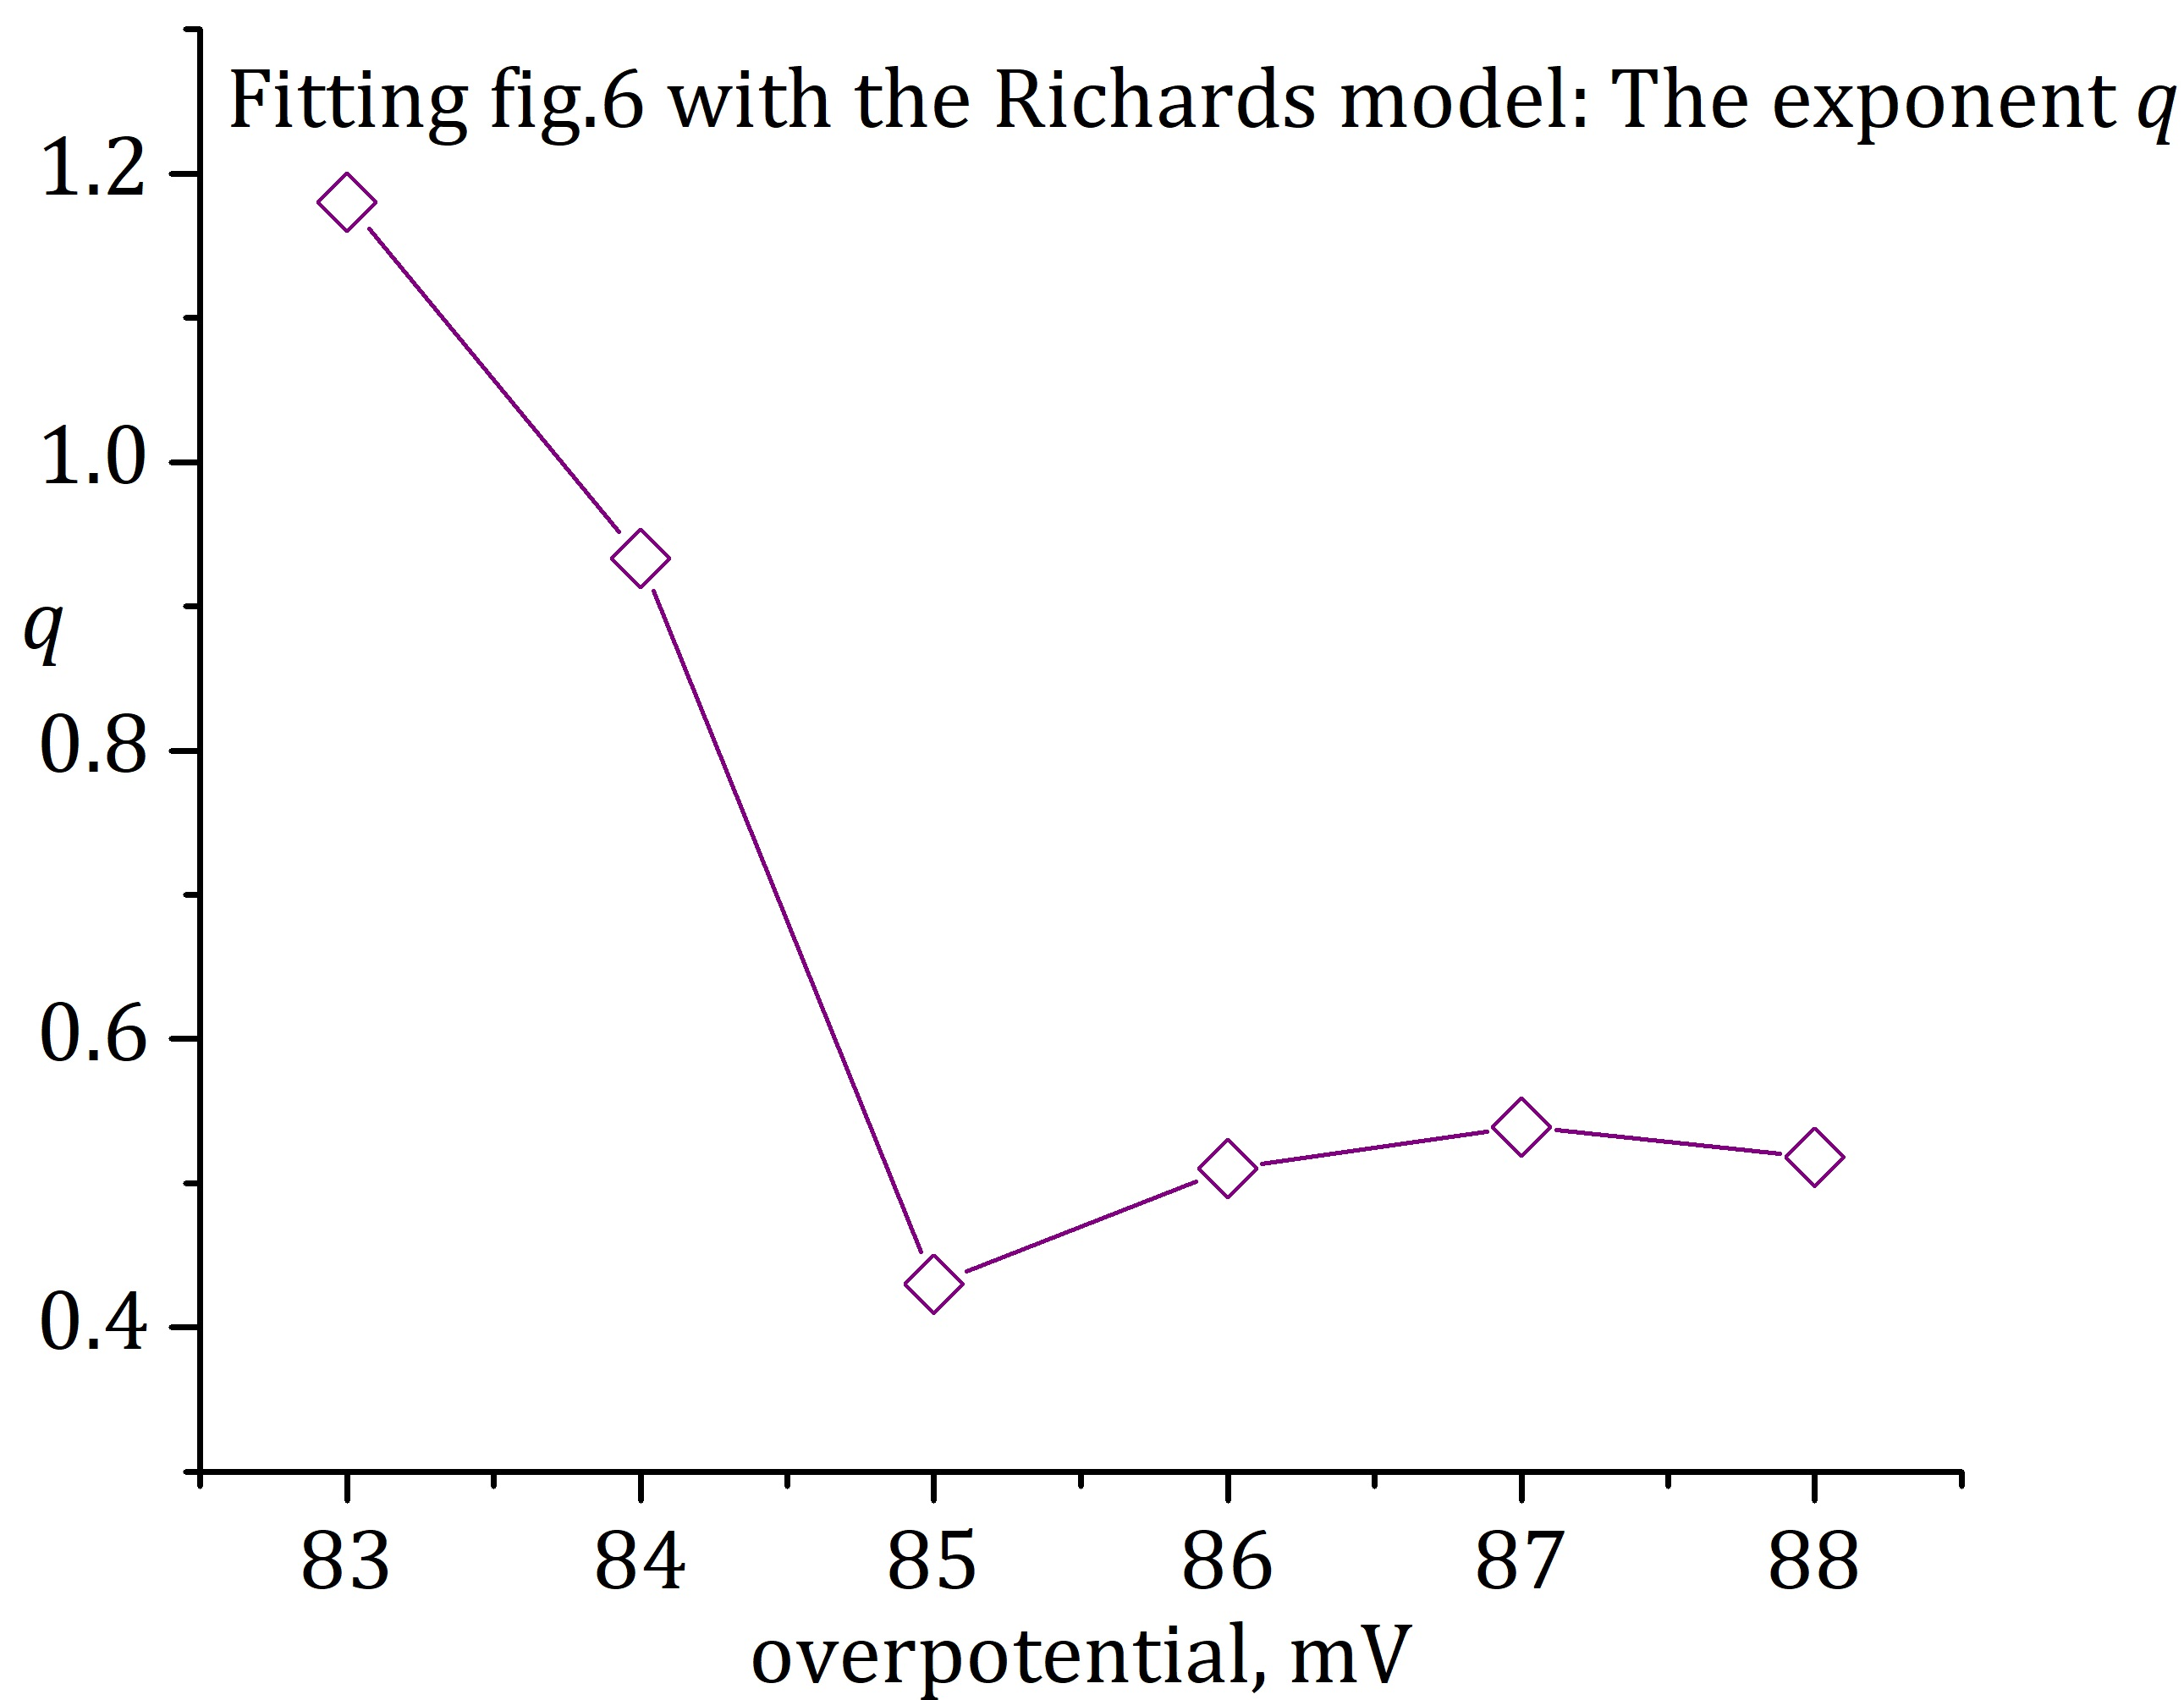
\includegraphics[width=0.43\textwidth]{ivan_markov_graphs/Fig6_Richads_q-oveporential.jpg}}
    \caption{Зависимост на параметъра $q$ от модела на Ричардс от свръхпотенциала}
\end{figure}
\begin{figure}[H]
    \centering
        \subfloat[Фиг. 5]{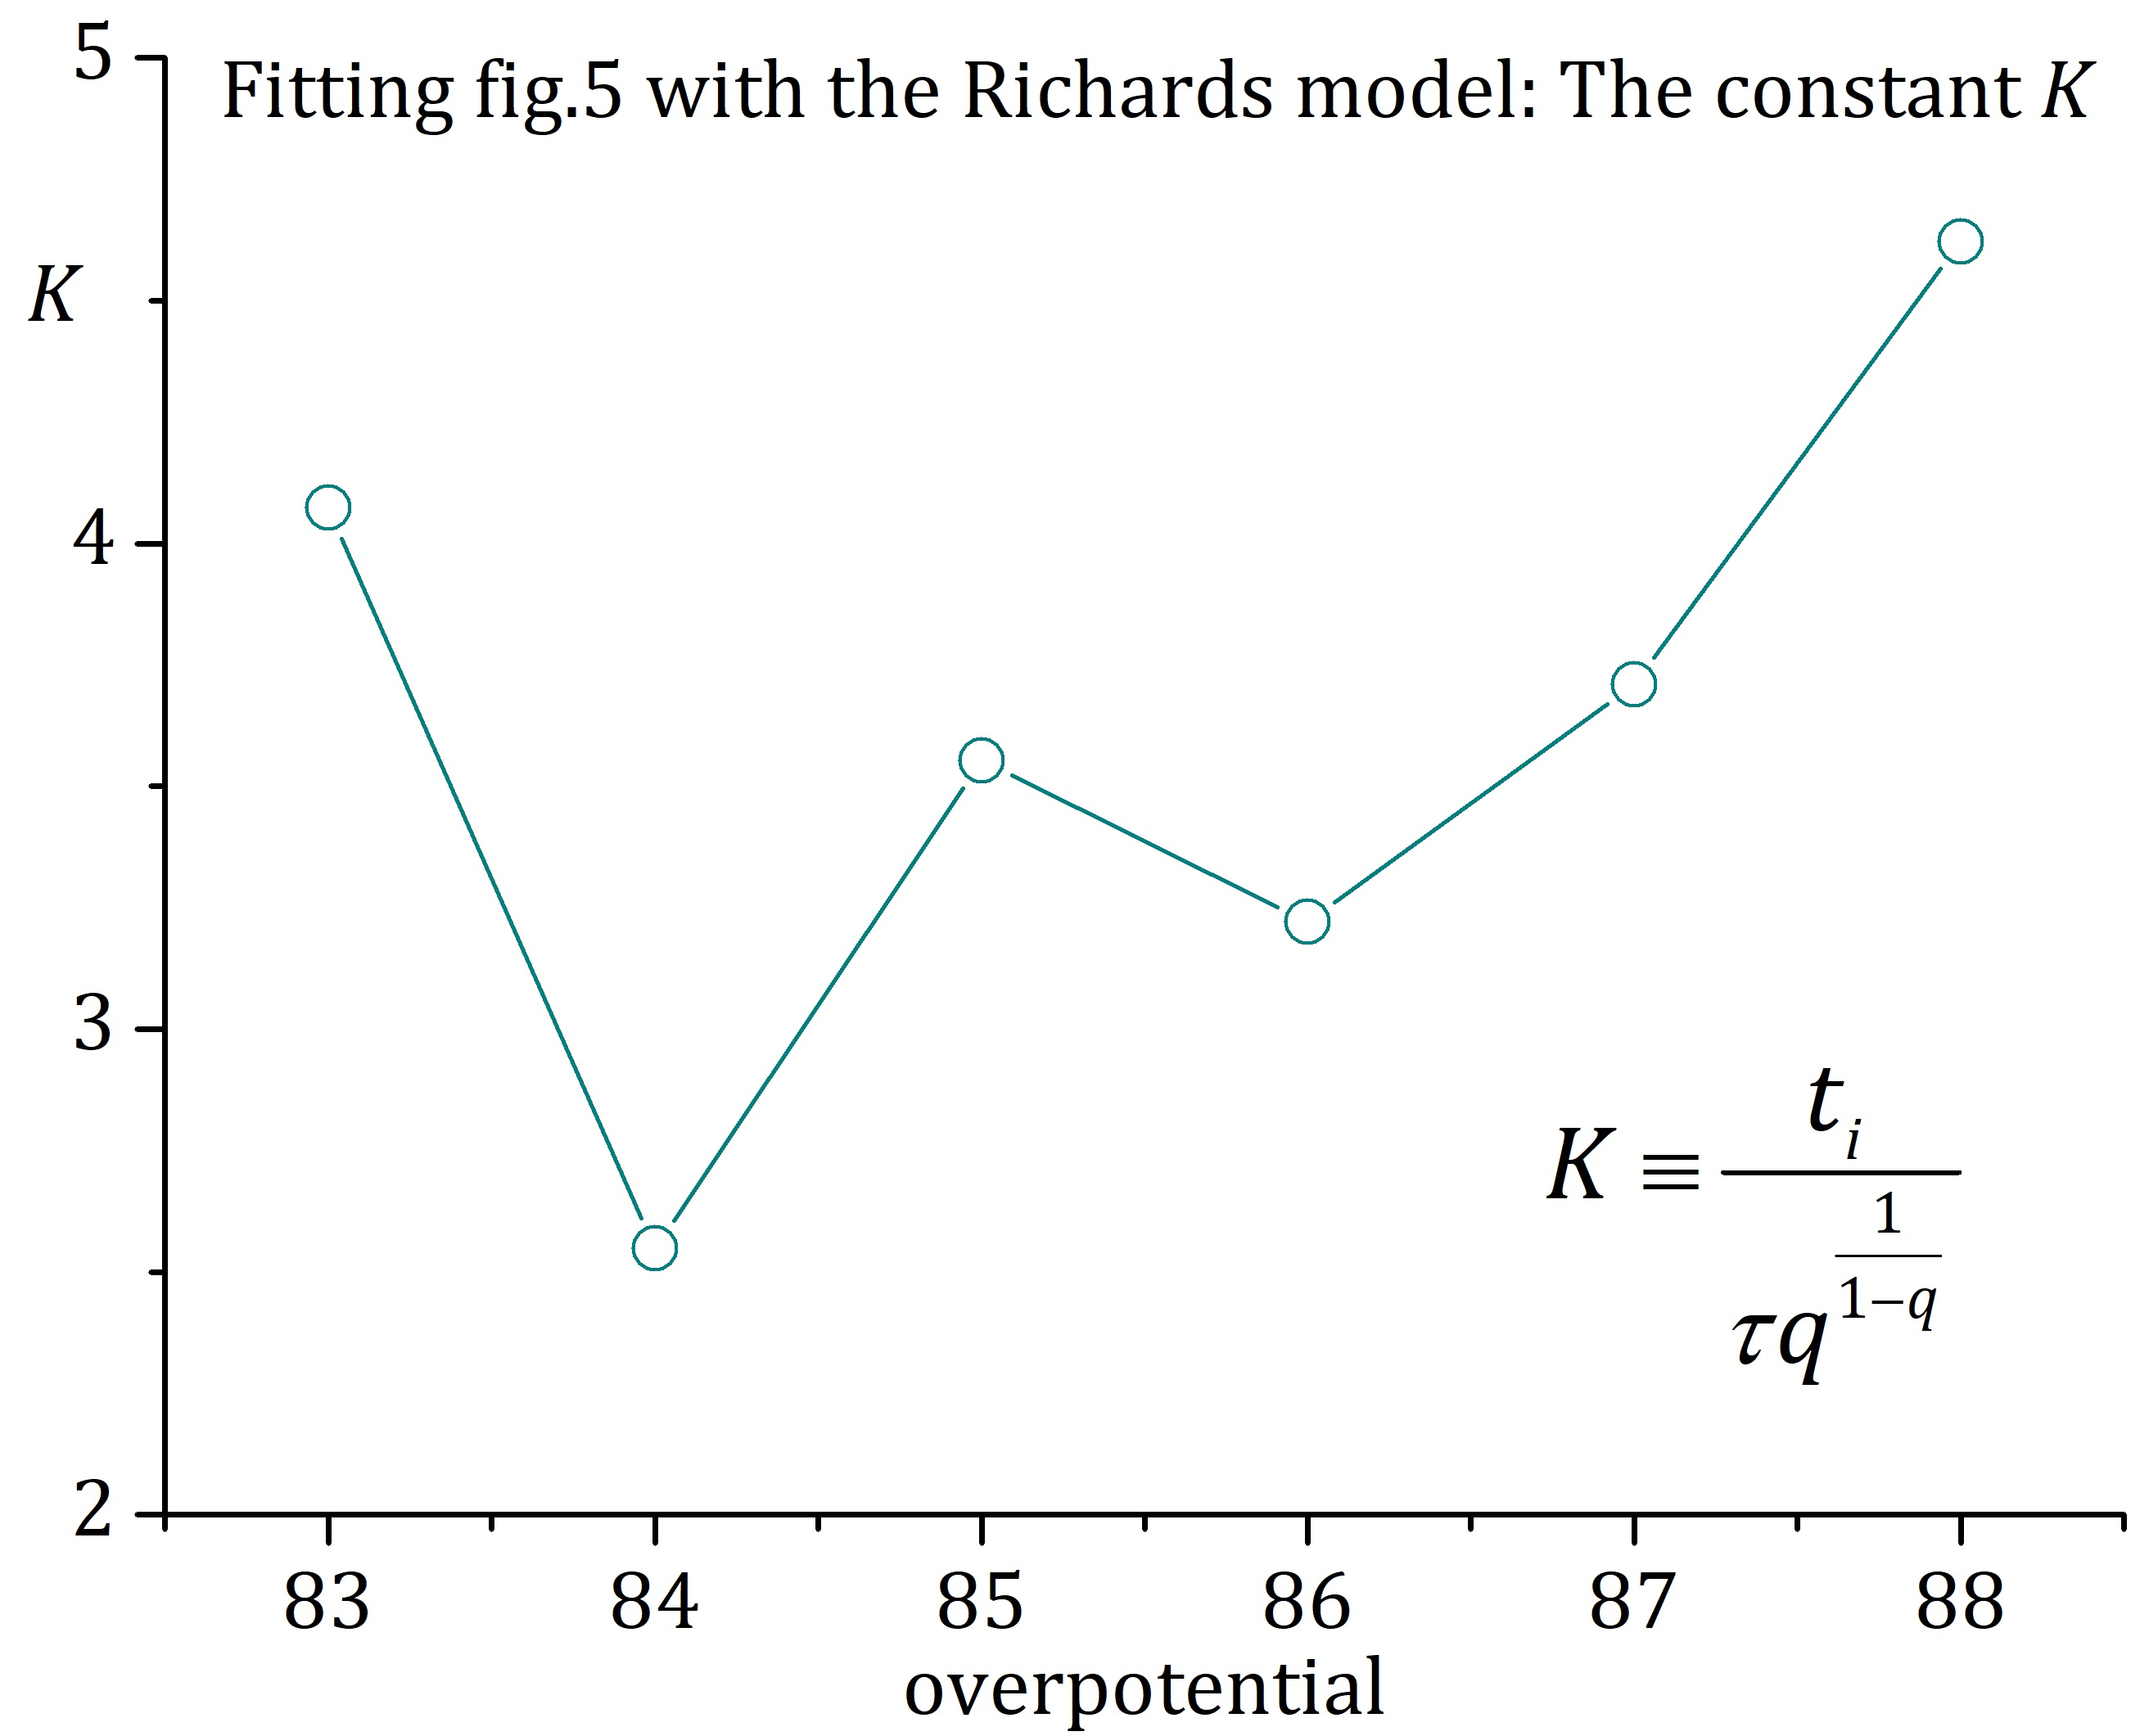
\includegraphics[width=0.45\textwidth]{ivan_markov_graphs/Fig5_K-overpotential.jpg}}
        \subfloat[Фиг. 6]{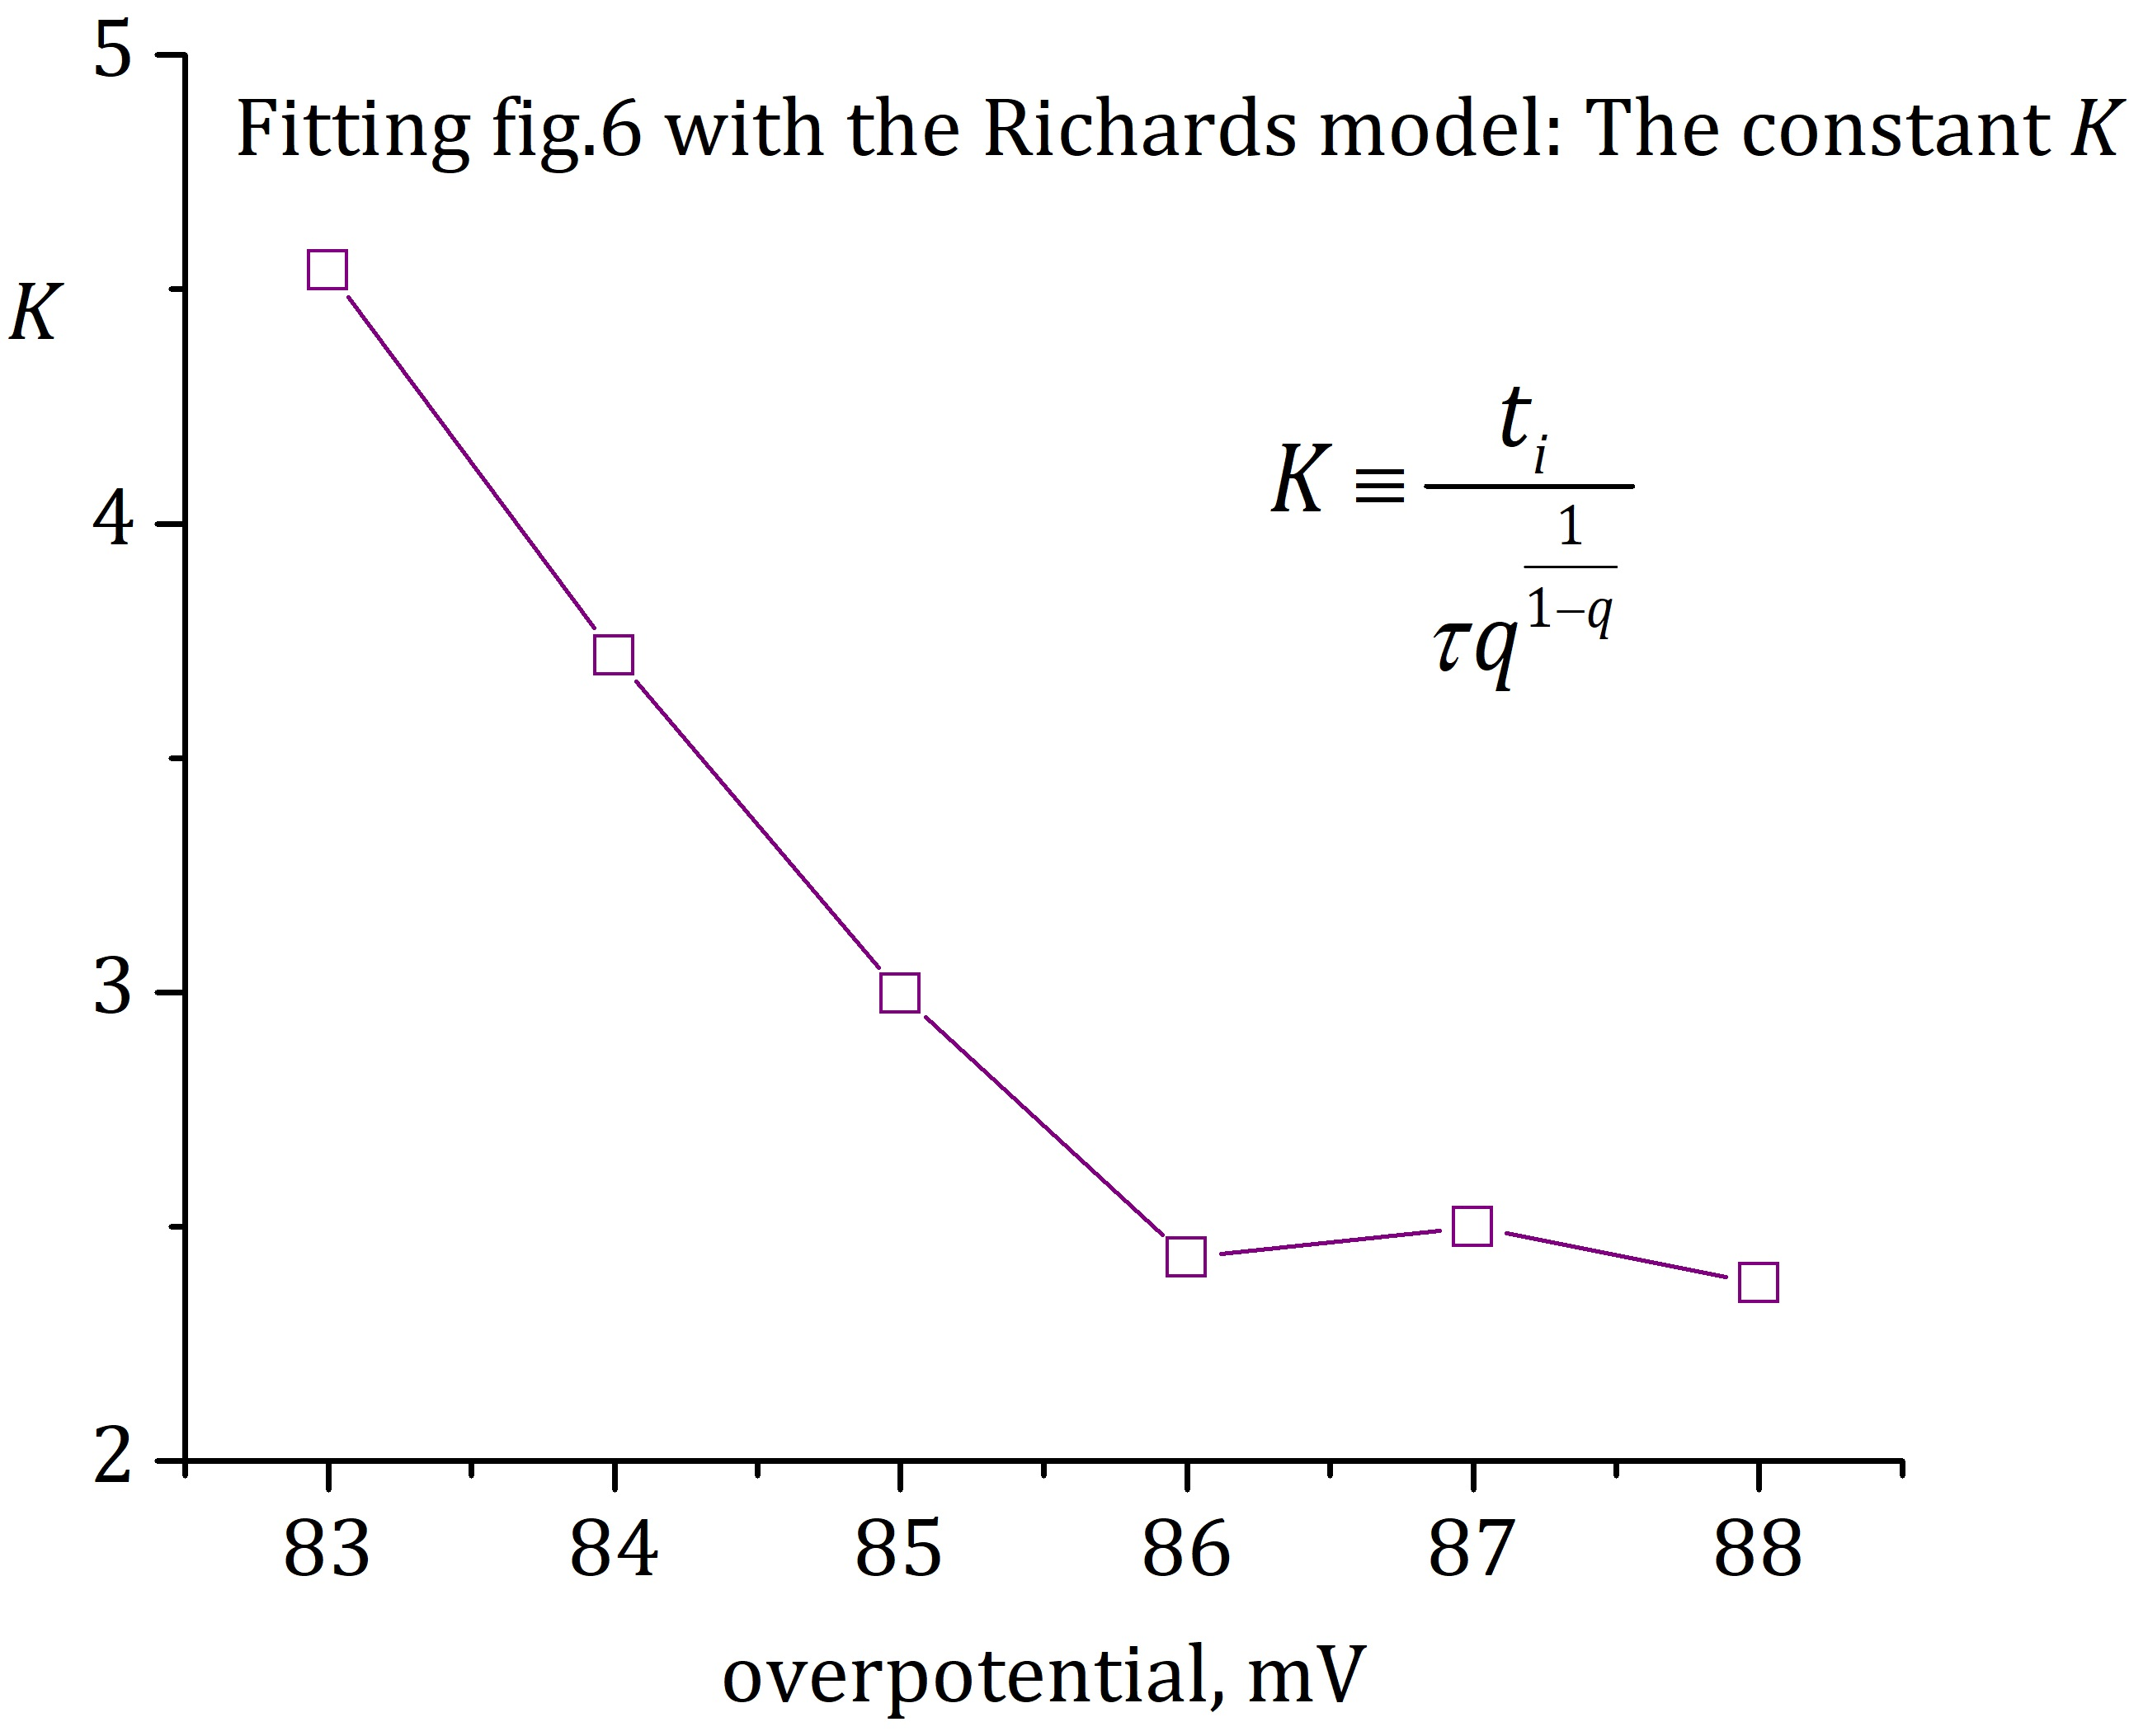
\includegraphics[width=0.45\textwidth]{ivan_markov_graphs/Fig6_K-overpotential.jpg}}
    \caption{Зависимост на параметъра $K$ от модела на Ричардс от свръхпотенциала}
\end{figure}

Важно е да отбележим, че на \autoref{fig:richards_rescaled} няма универсална крива, тъй като пареметрите $q, K$ на модела са различни за всеки набор данни.
\subsubsection{JMAKn}
\begin{figure}[H]
    \centering
        \subfloat[Фиг. 5]{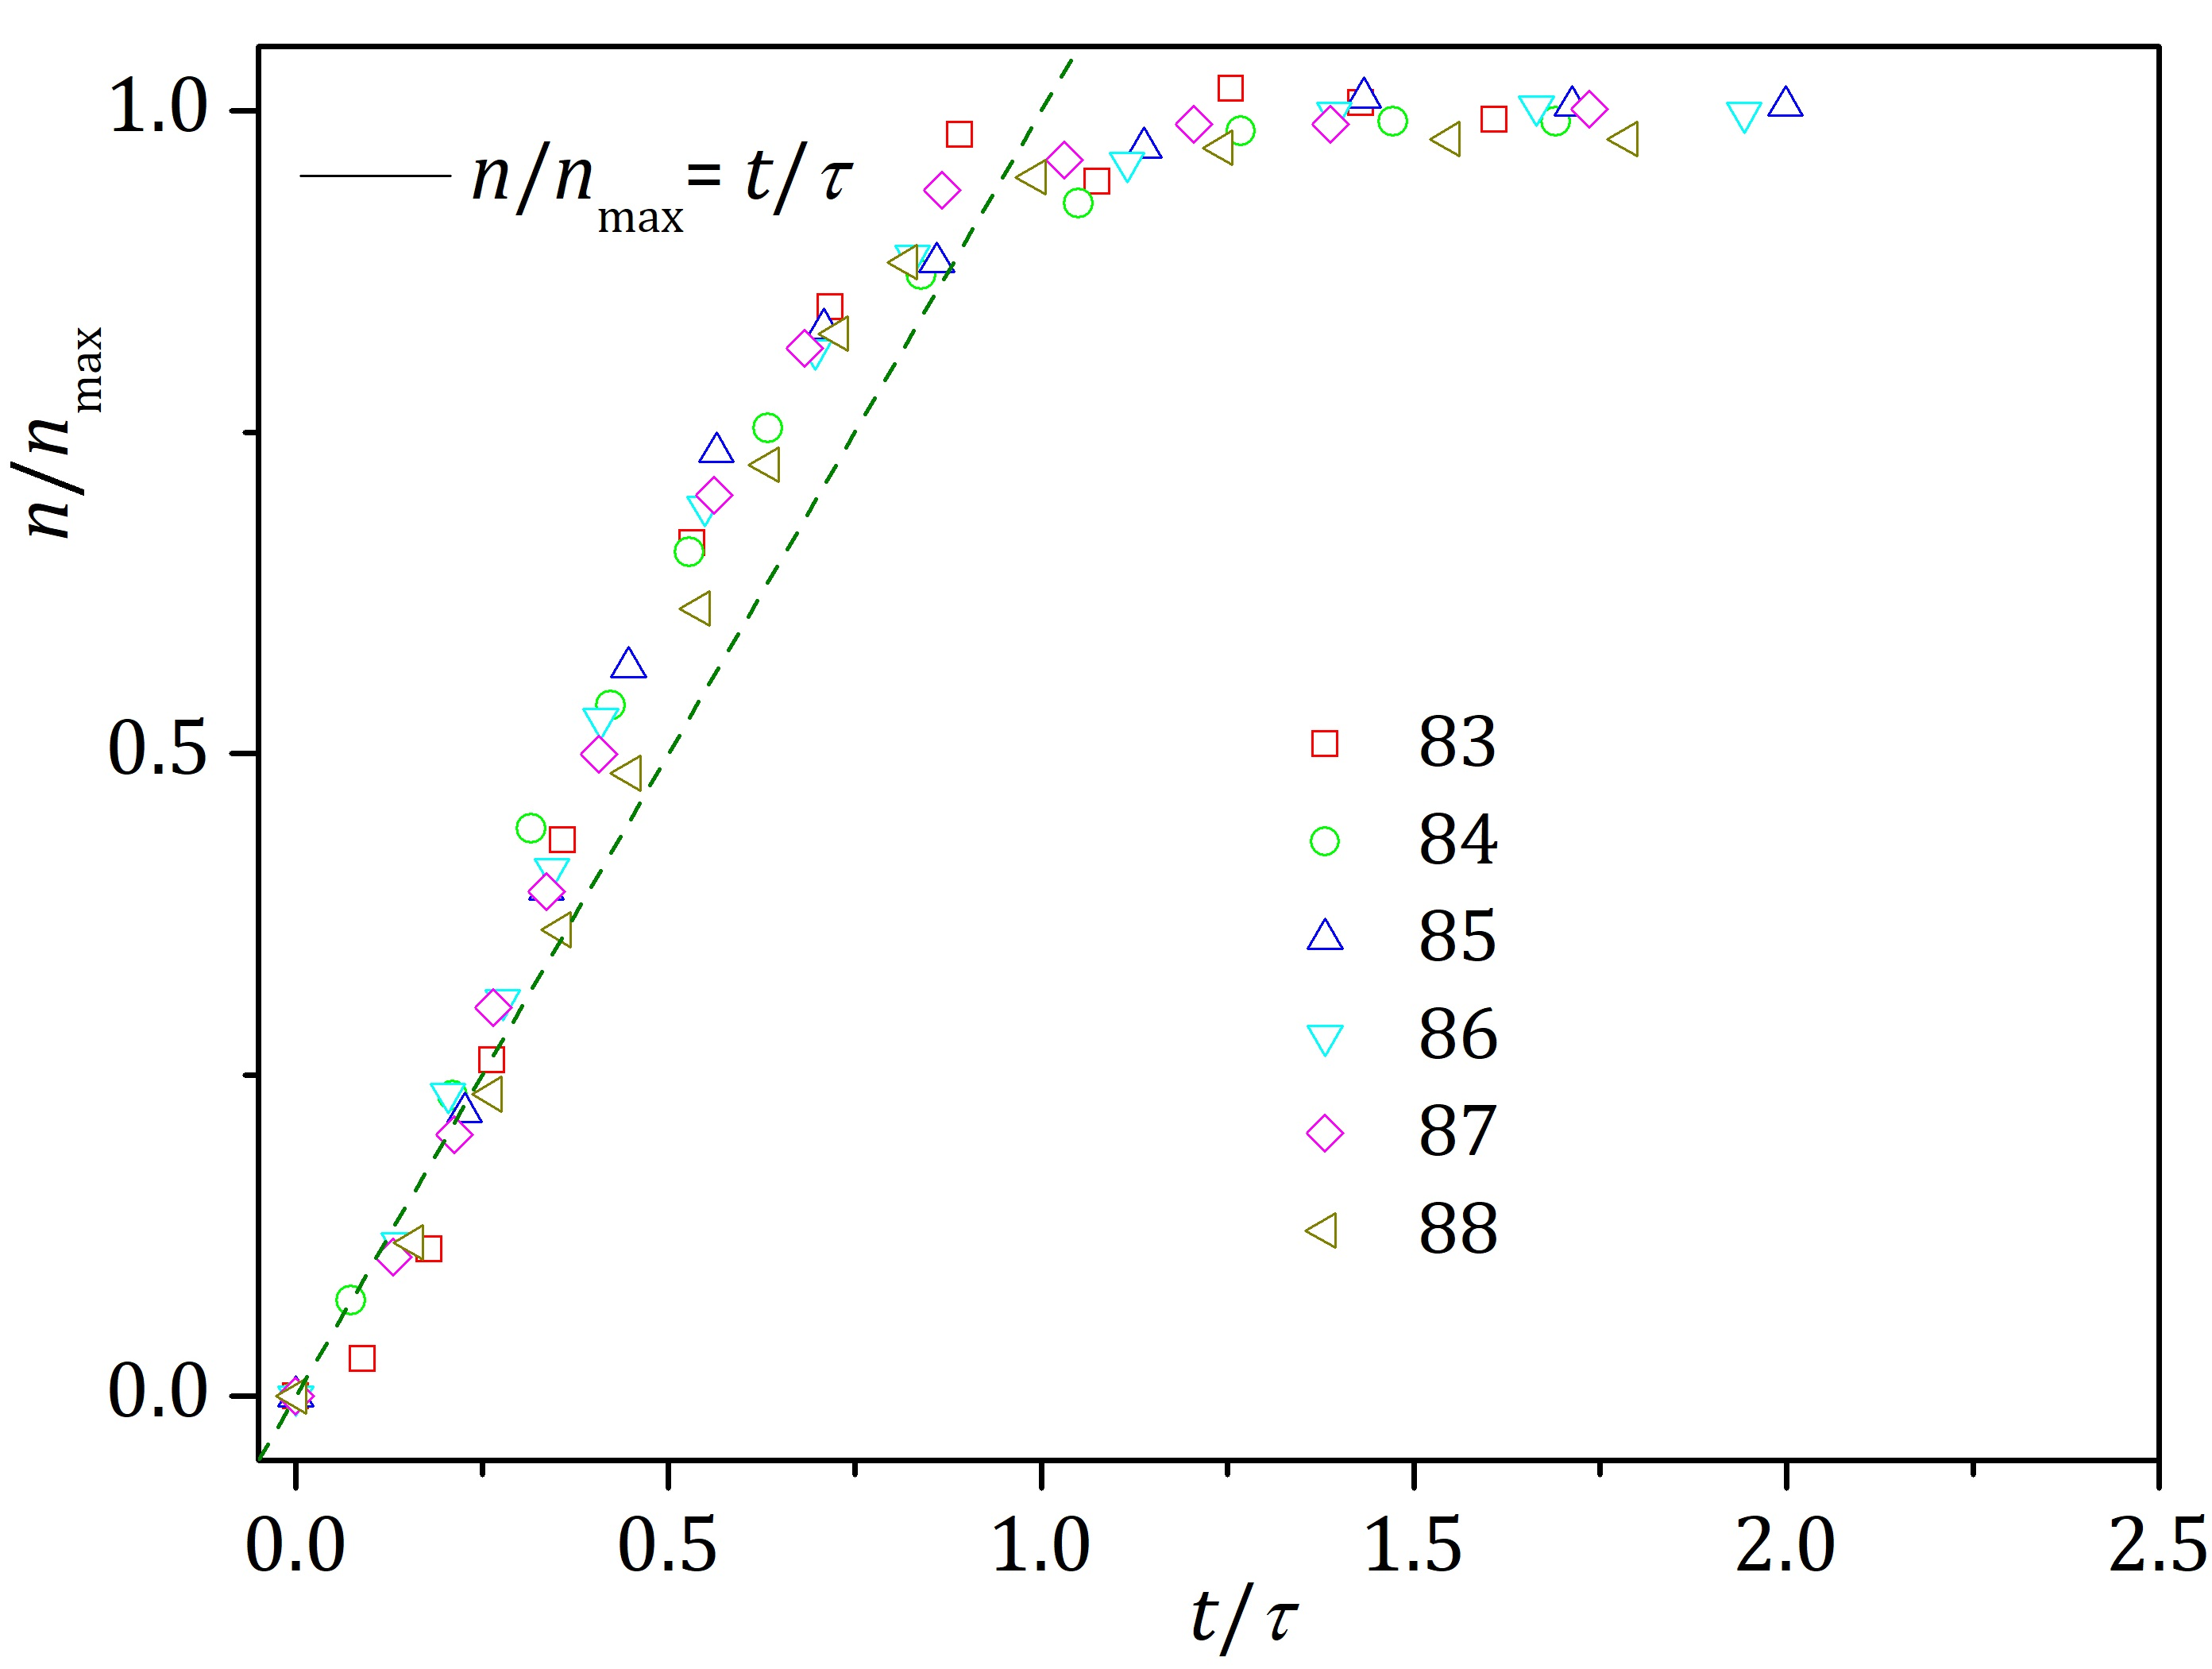
\includegraphics[width=0.48\textwidth]{ivan_markov_graphs/Fig5-jmak_rescaled.jpg}}
        \subfloat[Фиг. 6]{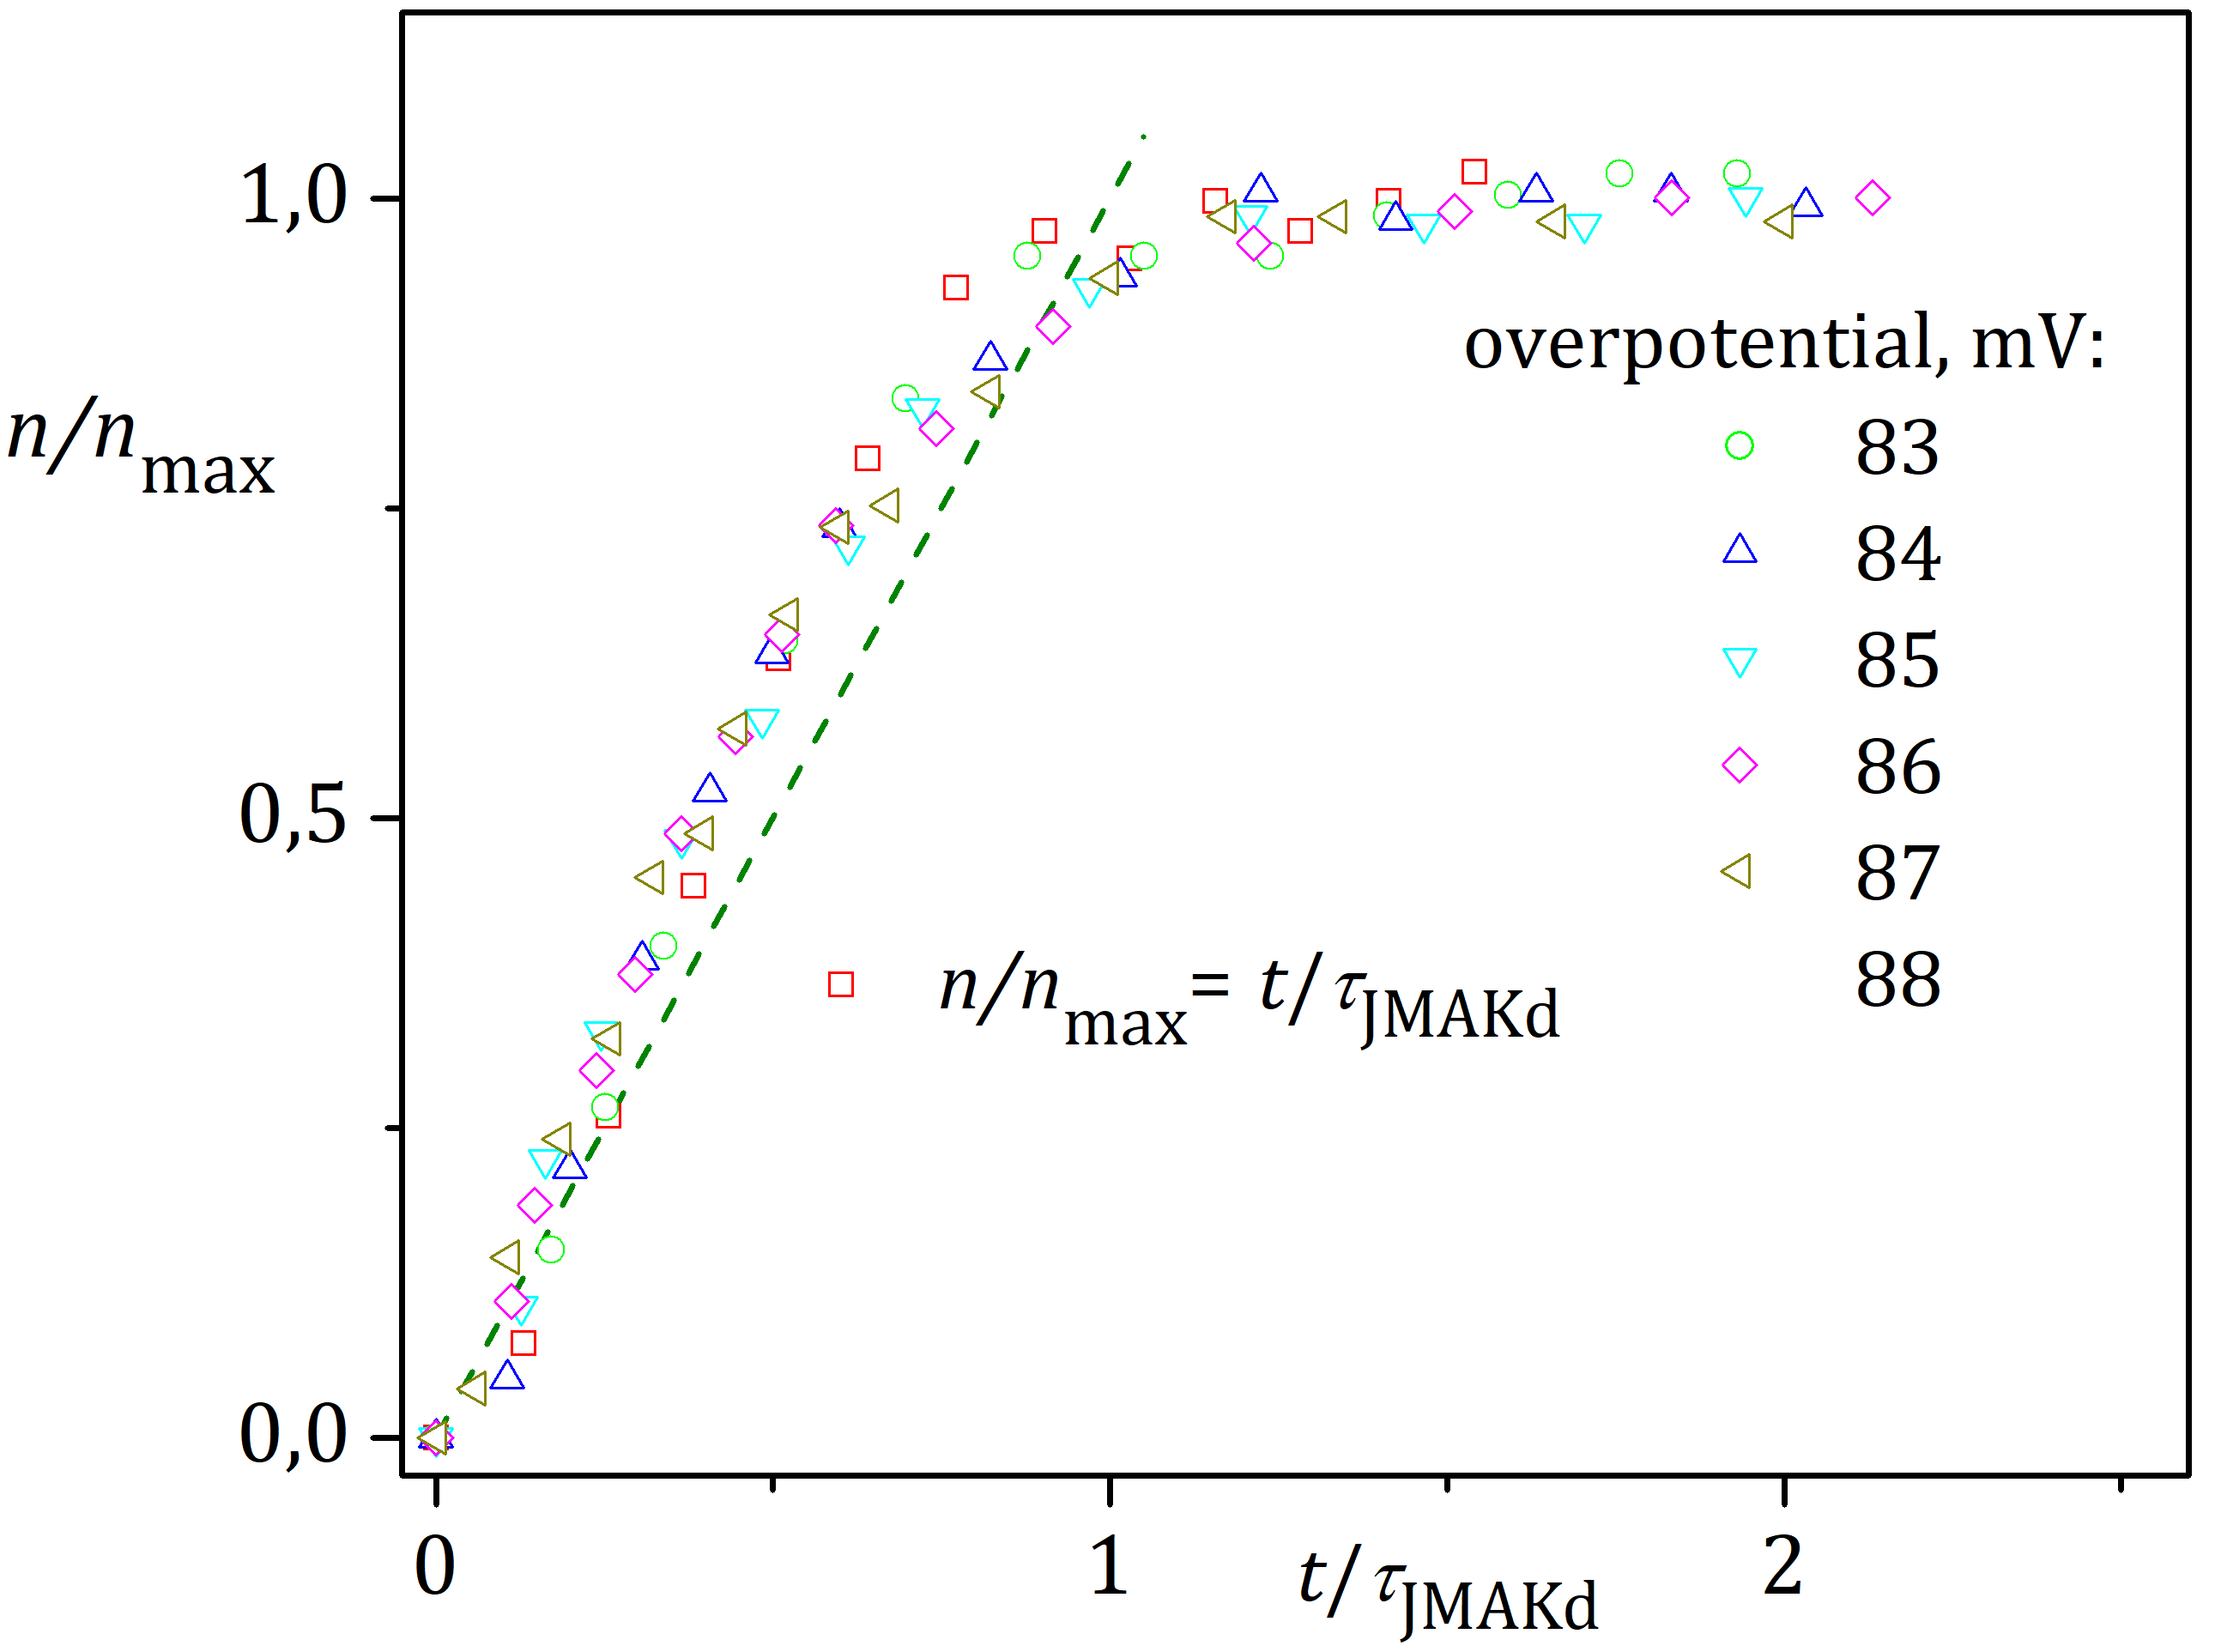
\includegraphics[width=0.48\textwidth]{ivan_markov_graphs/Fig6-jmak_rescaled.png}}
    \caption{Рескалирани данни от JMAKn за различни свръхпотенциали}
\end{figure}
%% TODO: ADD REFERENCE TO TABLE WITH DATA!!!!

Тук отново нямаме универсална крива, тъй като за различните набори данни $n$ е различно. Стойността им е в интервала $n \in [1.6, 1.9]$, т.е. $n \approx 2$. Това потвърждава в комбинация с \autoref{fig:nvsd_graph} изборът ни за $\alpha_{21}$ като най-прост модел, съдържащ само $N_{max}$ и времева скала като параметри.
%% TODO: FIX d to be n on graph!!!!!!!
\begin{figure}[H]
    \centering
        \subfloat[Фиг. 5]{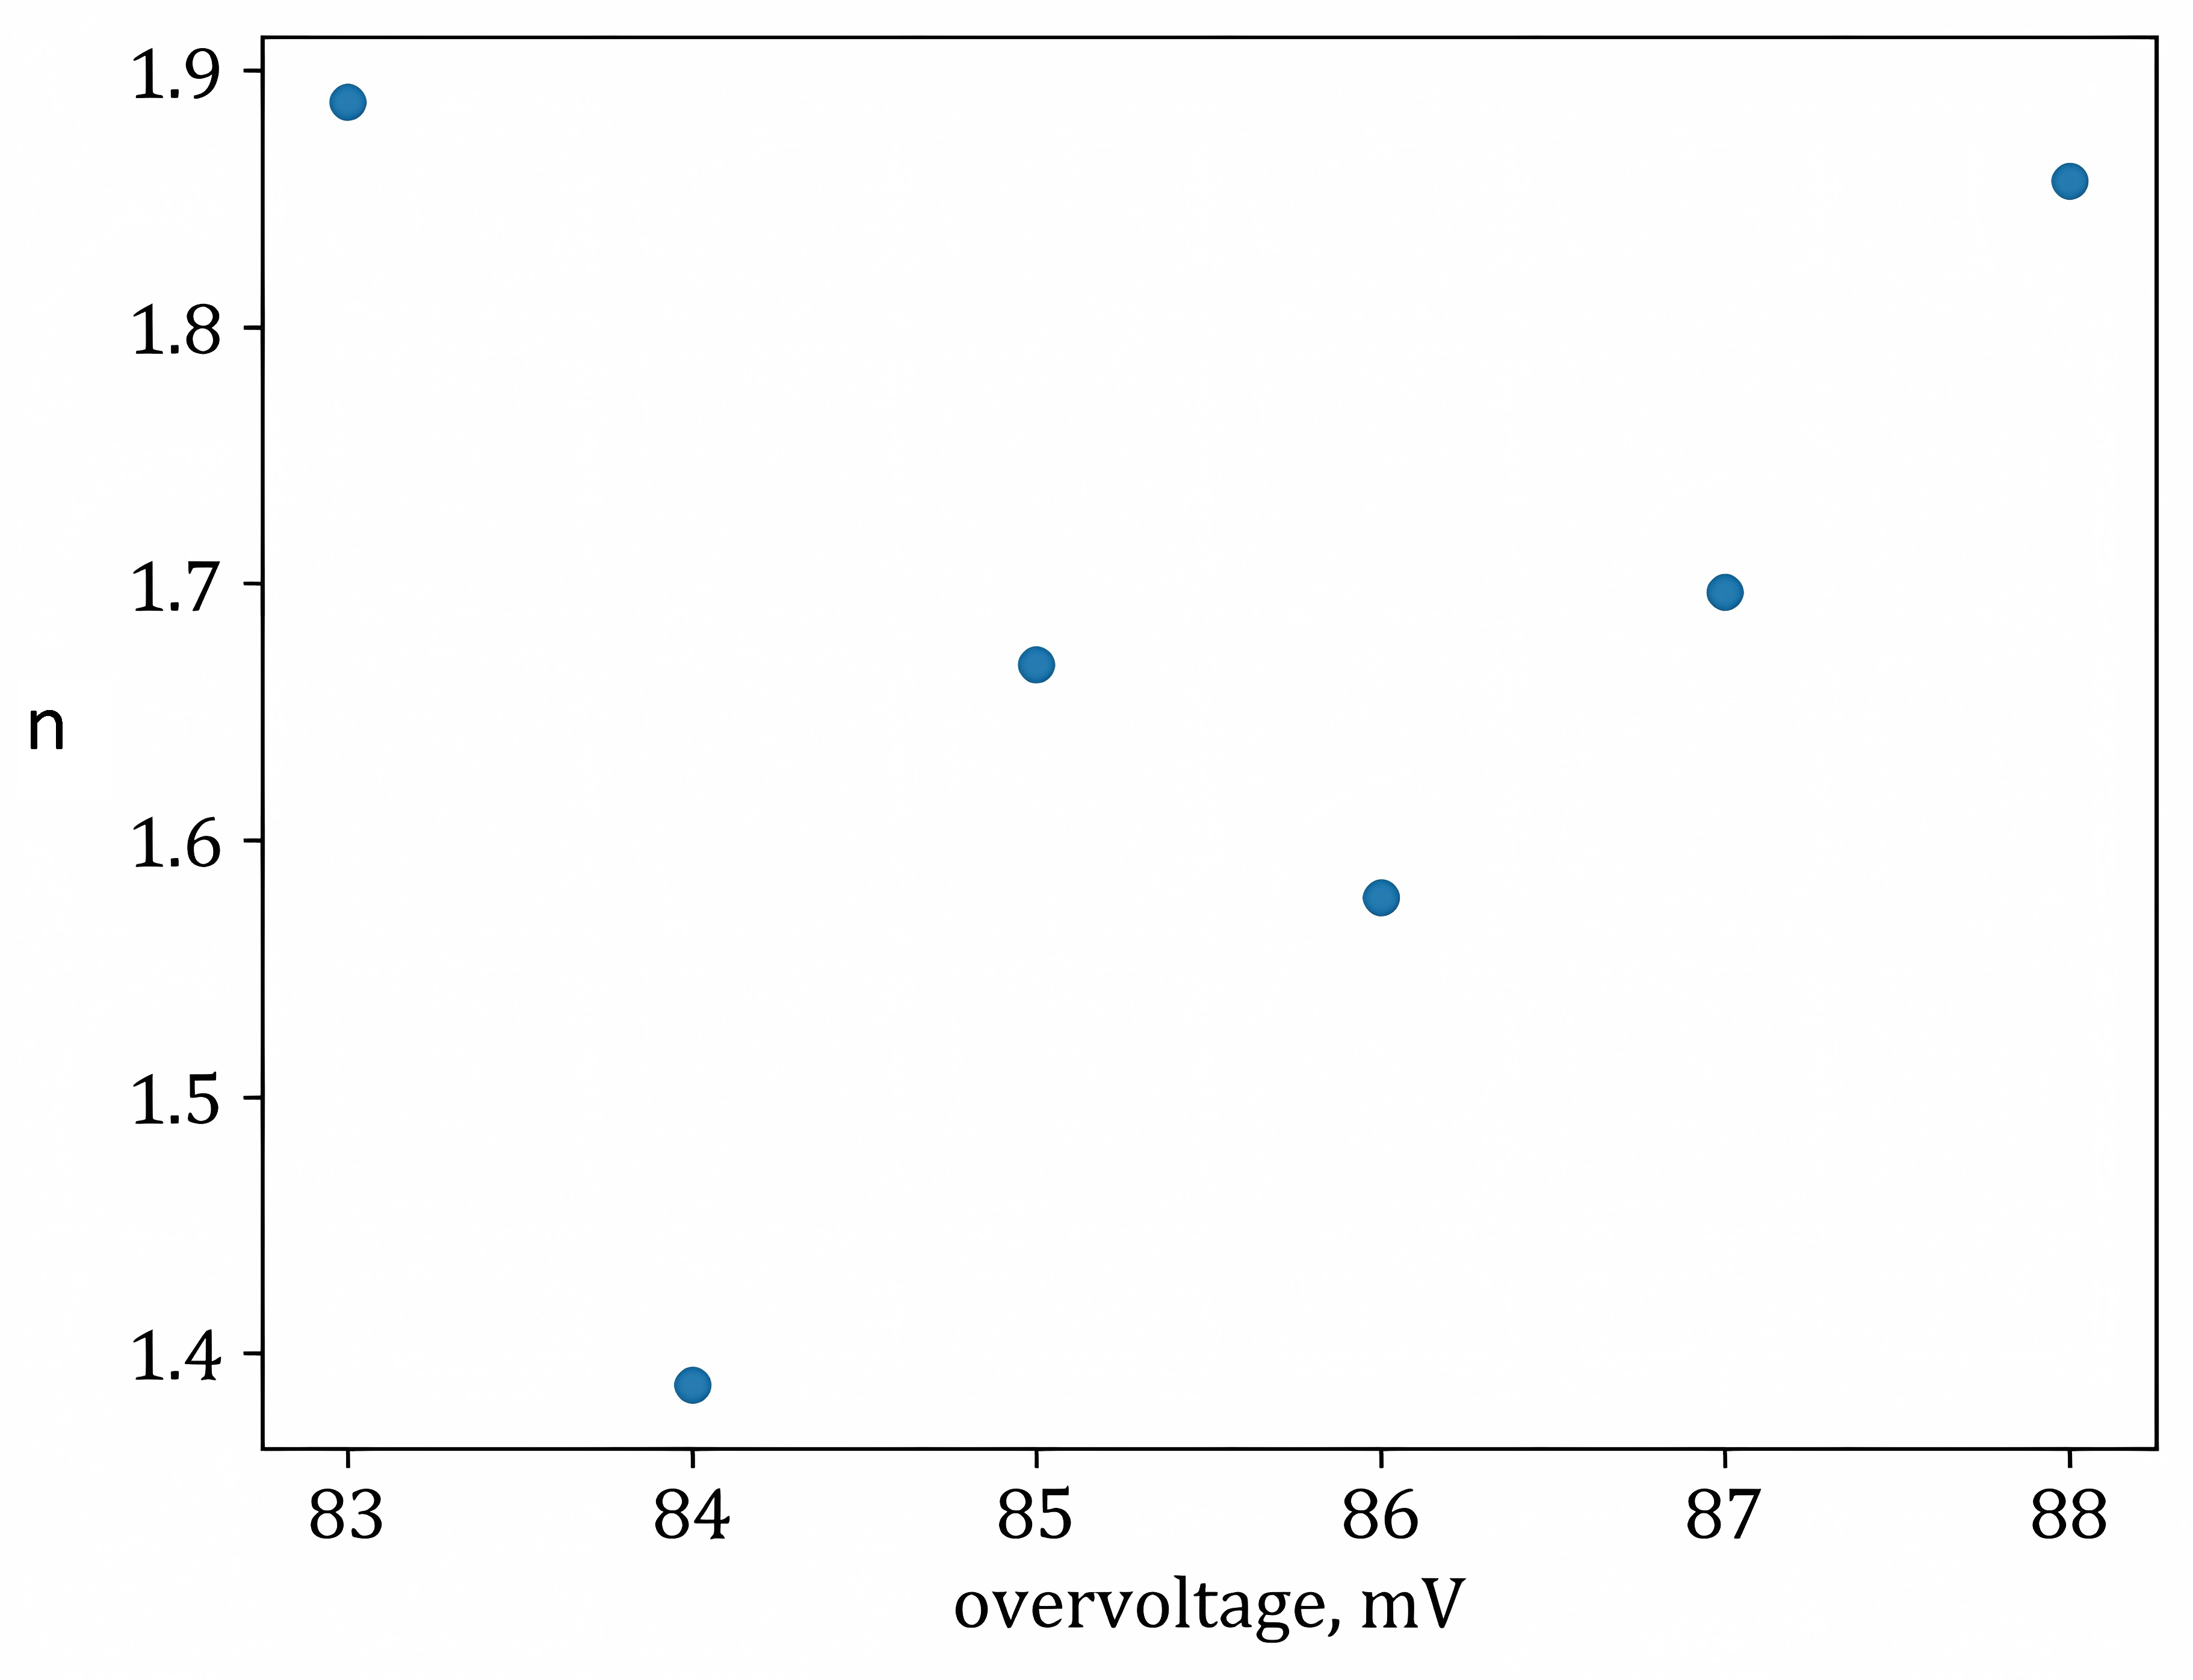
\includegraphics[width=0.48\textwidth]{ivan_markov_graphs/fig5_d_jmakn.png}}
        \subfloat[Фиг. 6]{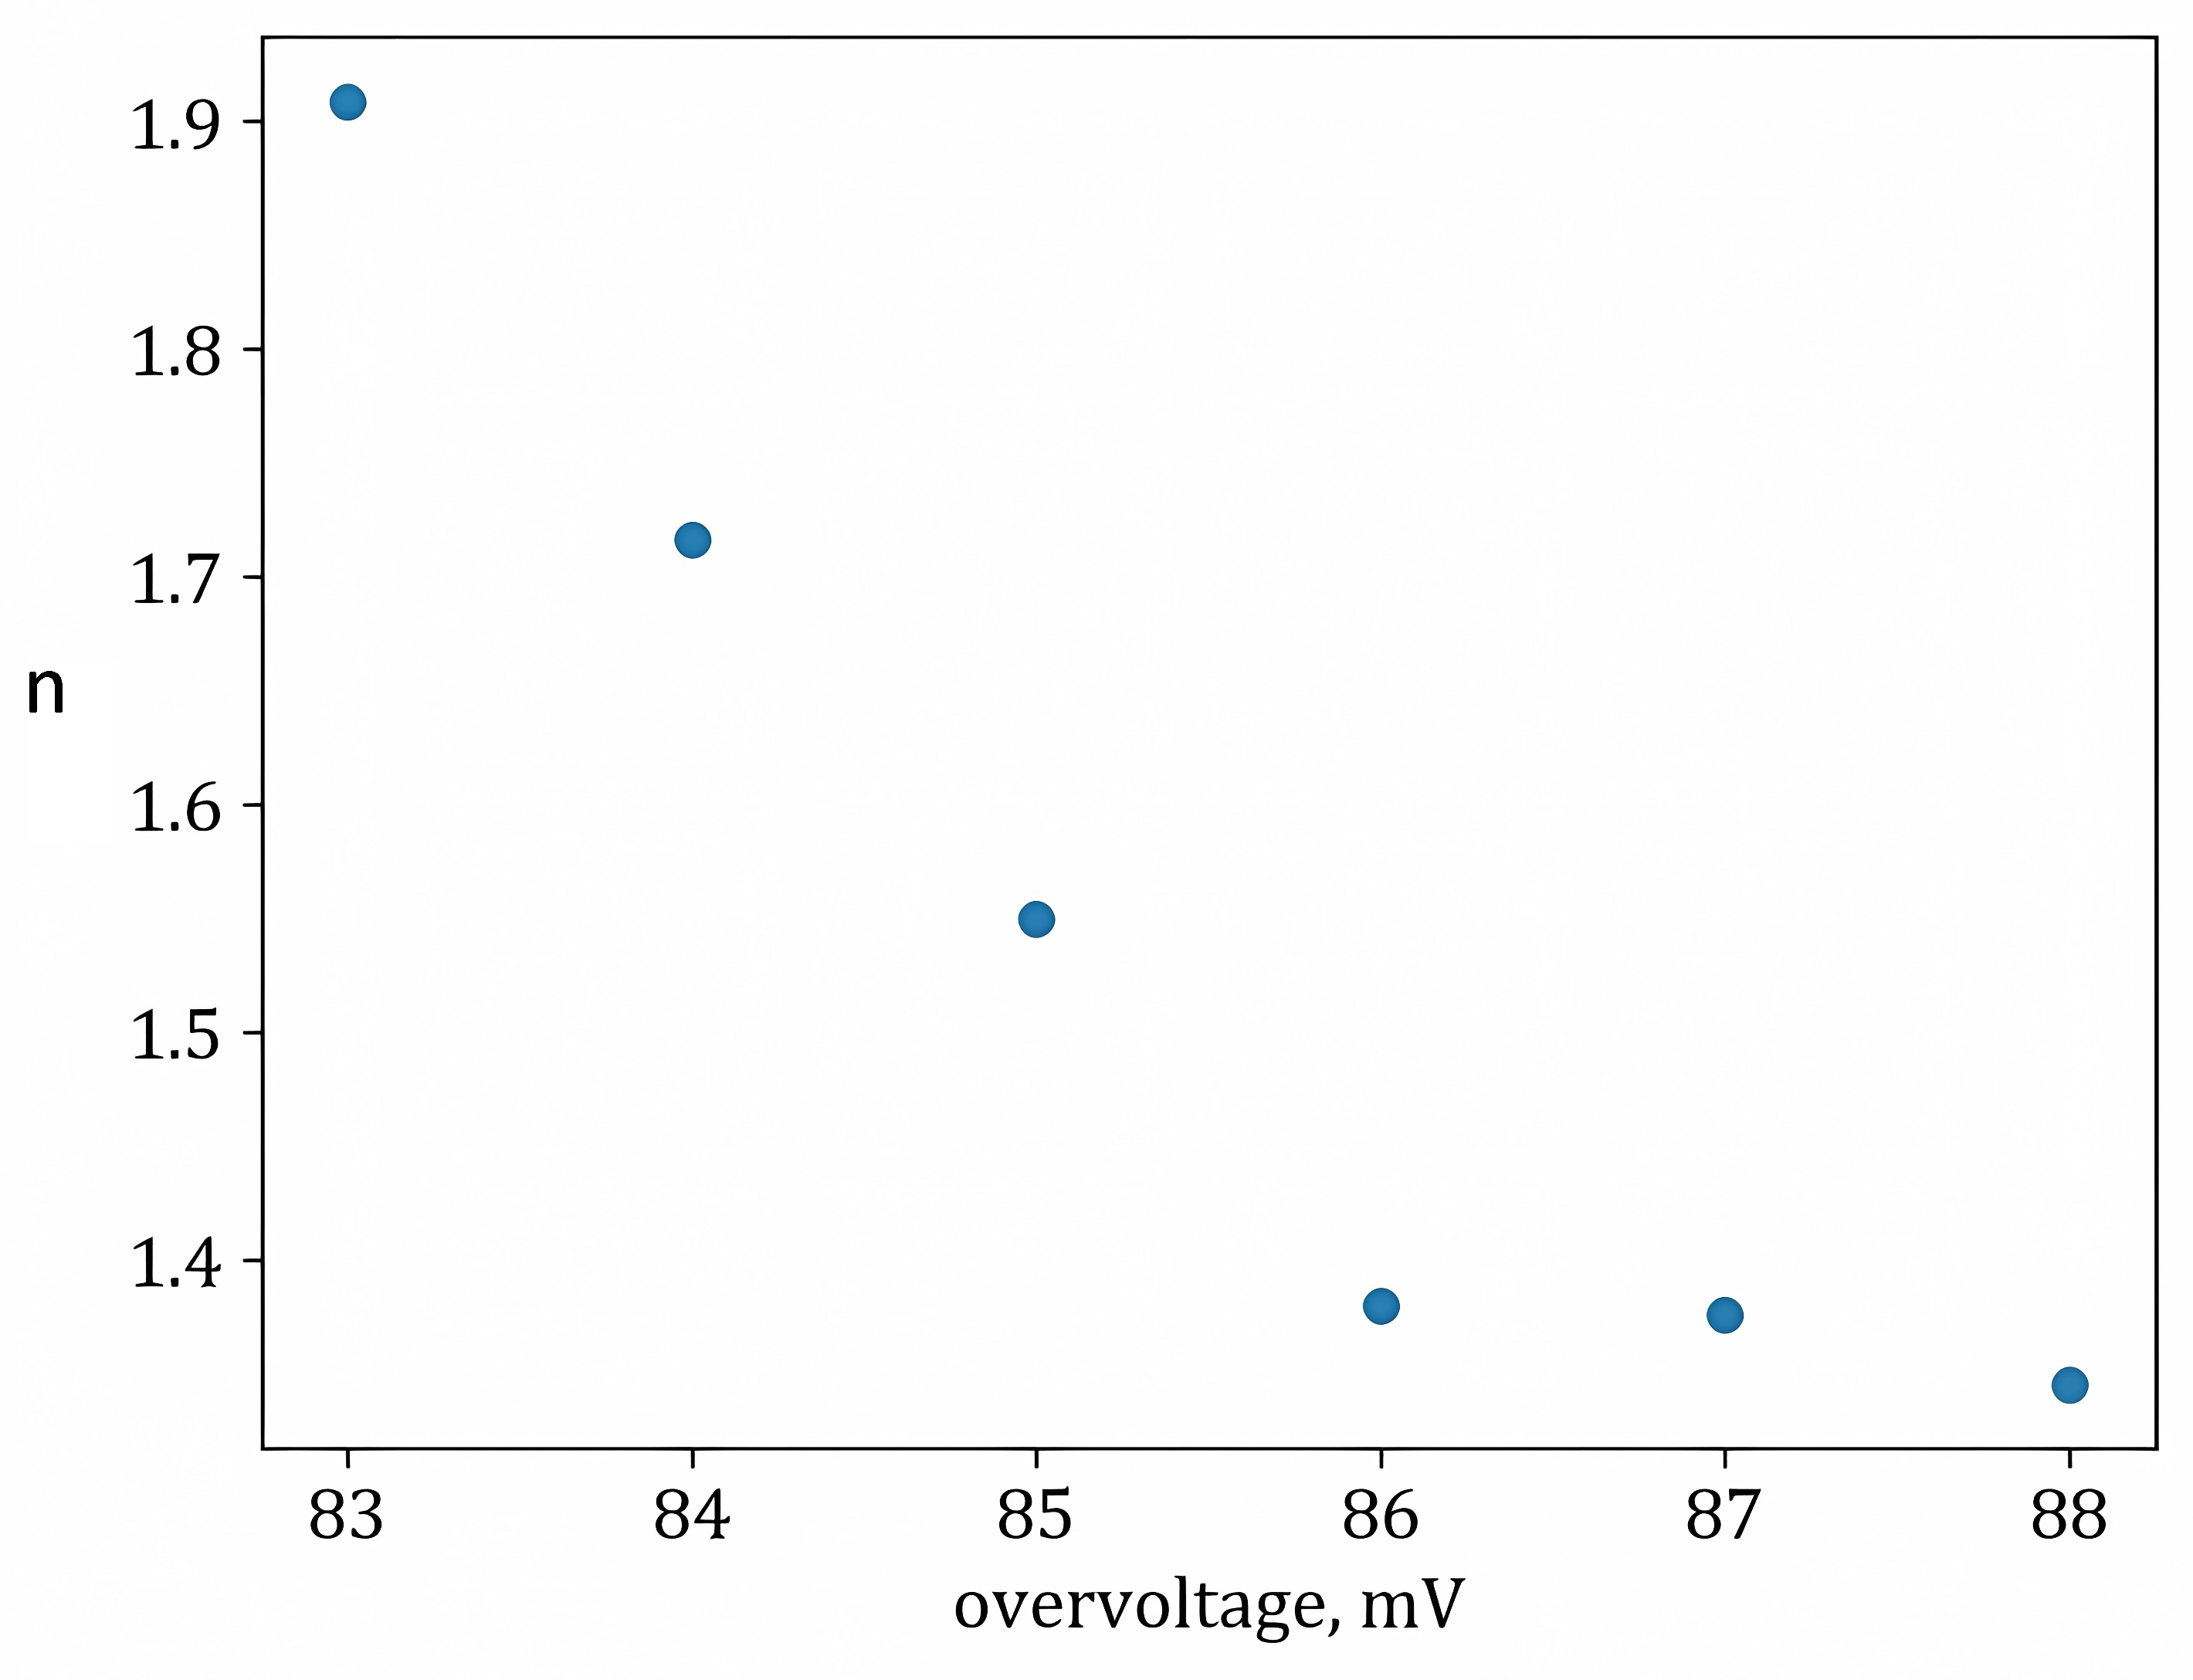
\includegraphics[width=0.48\textwidth]{ivan_markov_graphs/fig6_d_jmakn.png}}
    \caption{Стойности за параметъра $n$ от JMAKn}
\end{figure}
\begin{figure}[H]
    \centering
        \subfloat[Фиг. 5]{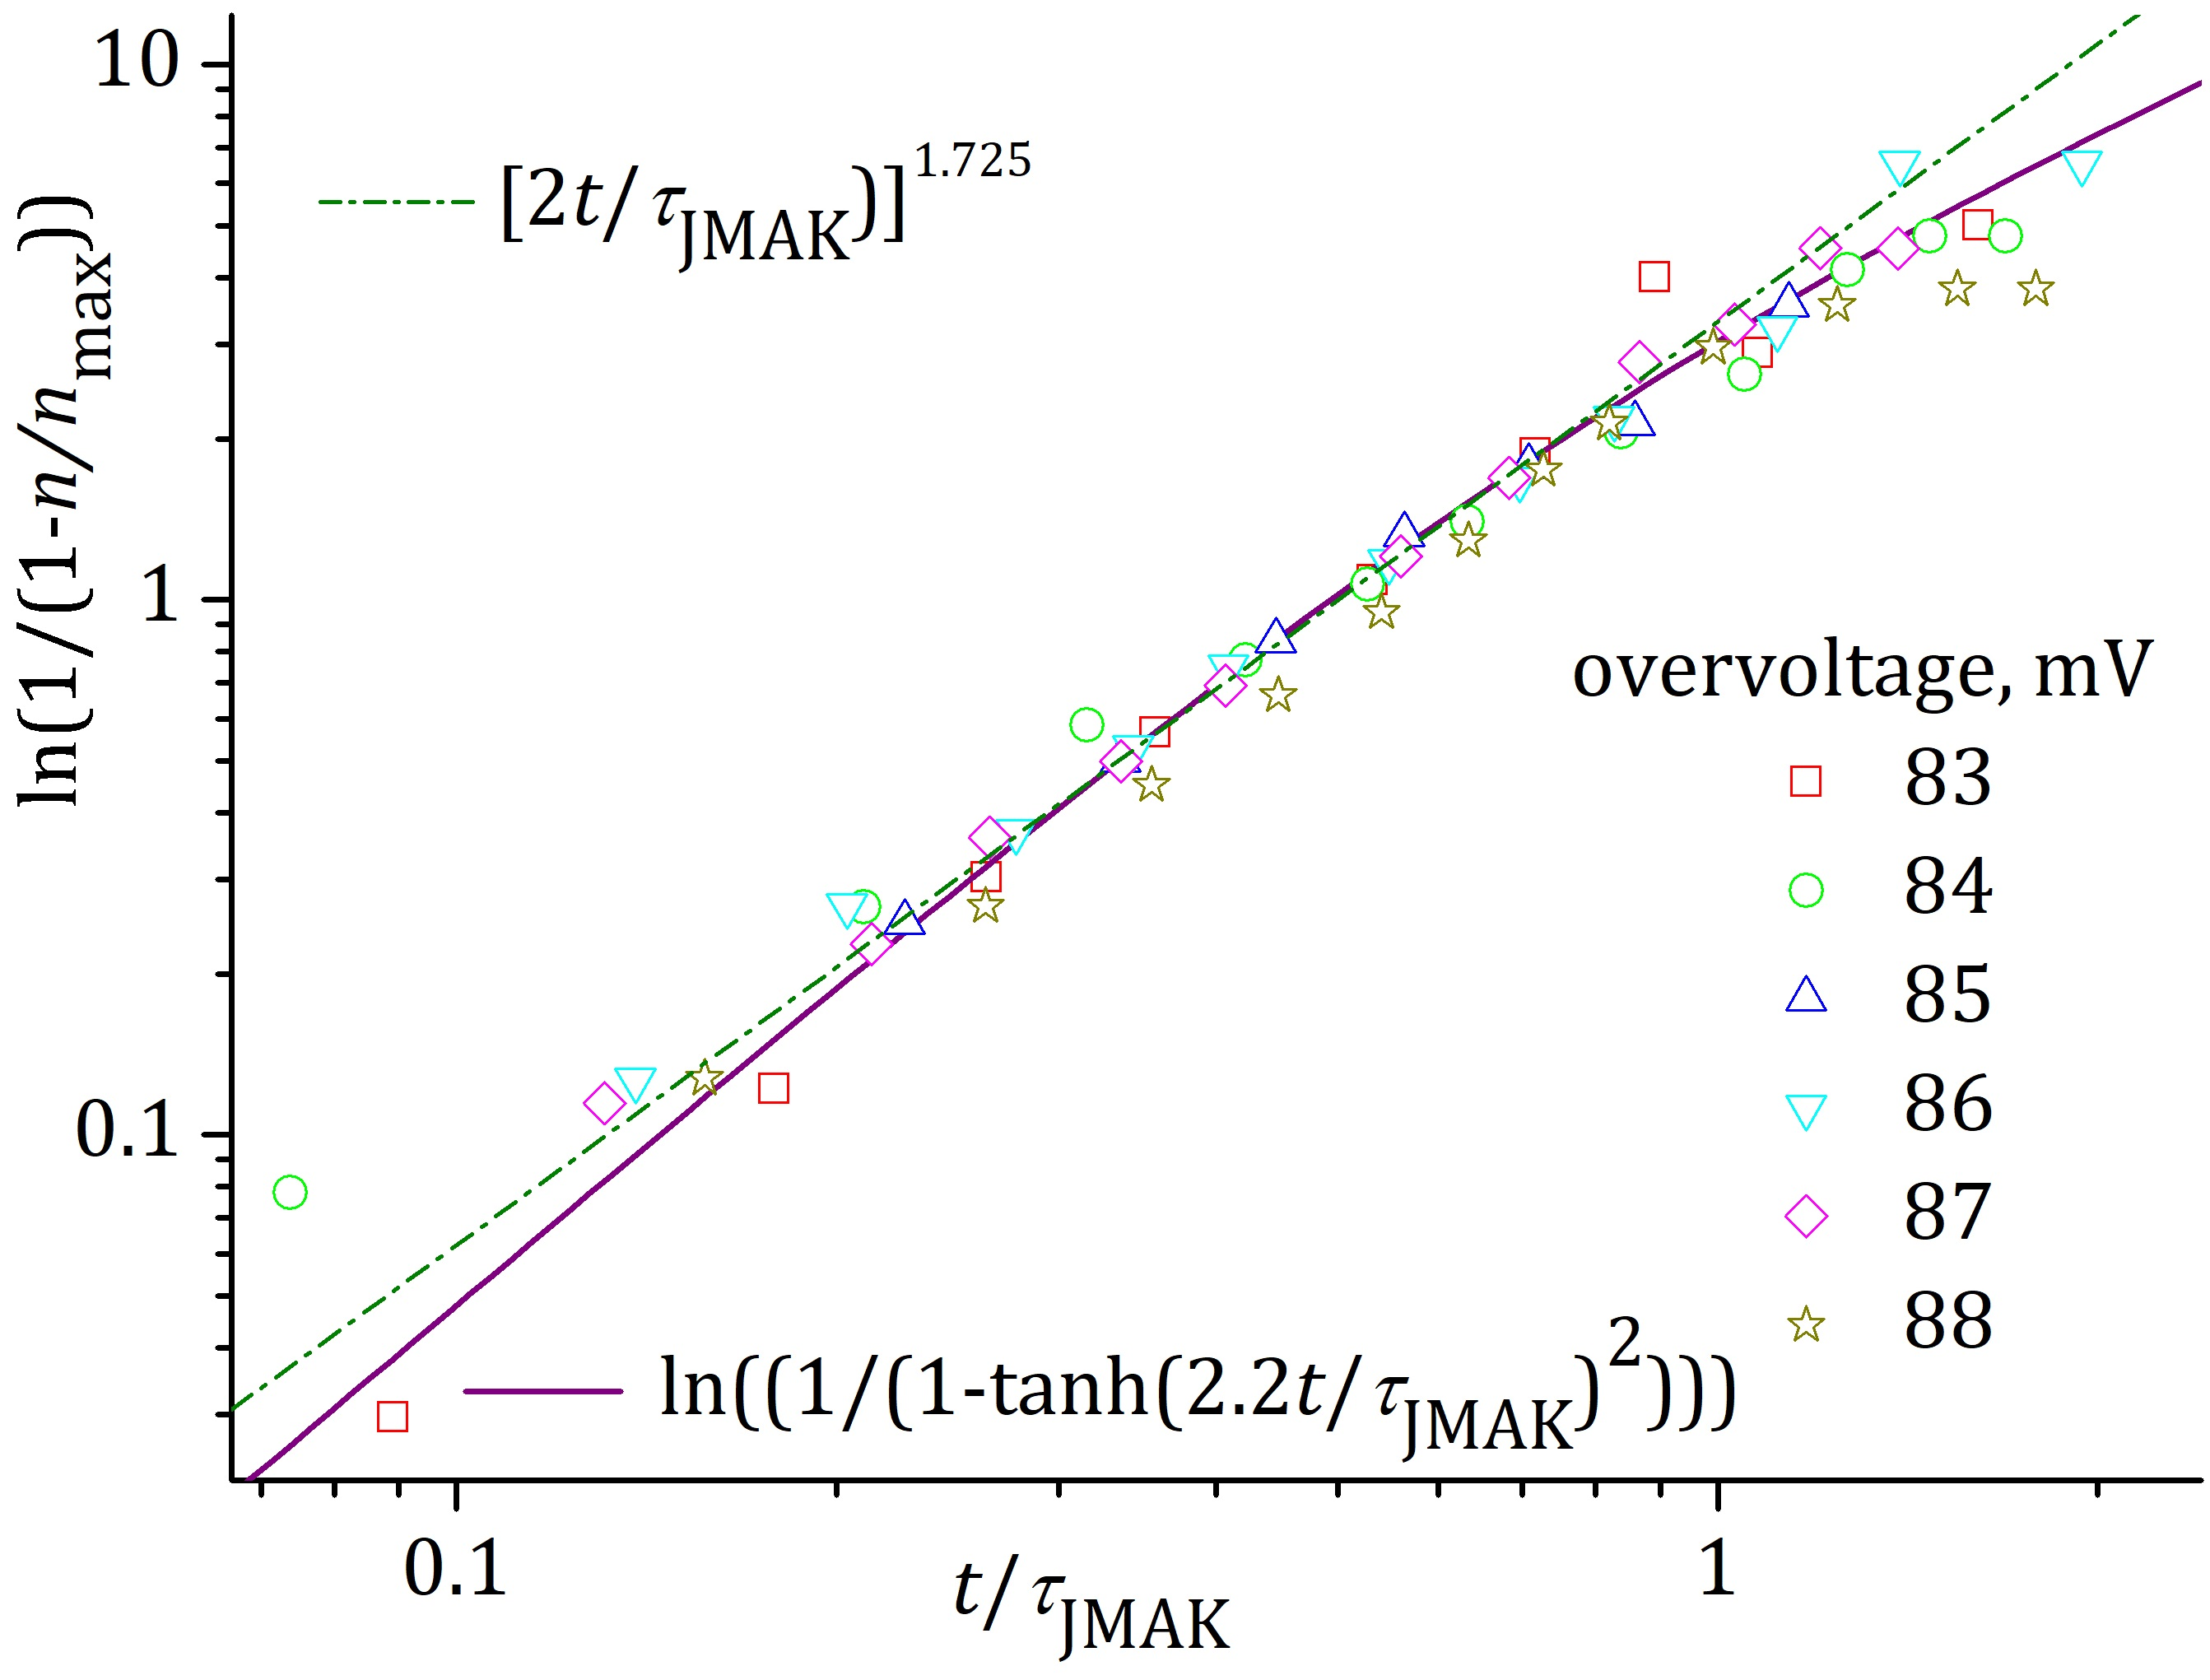
\includegraphics[width=0.48\textwidth]{ivan_markov_graphs/Fig5-jmak_rescaled_inAvramiCoordinates.jpg}}
        \subfloat[Фиг. 6]{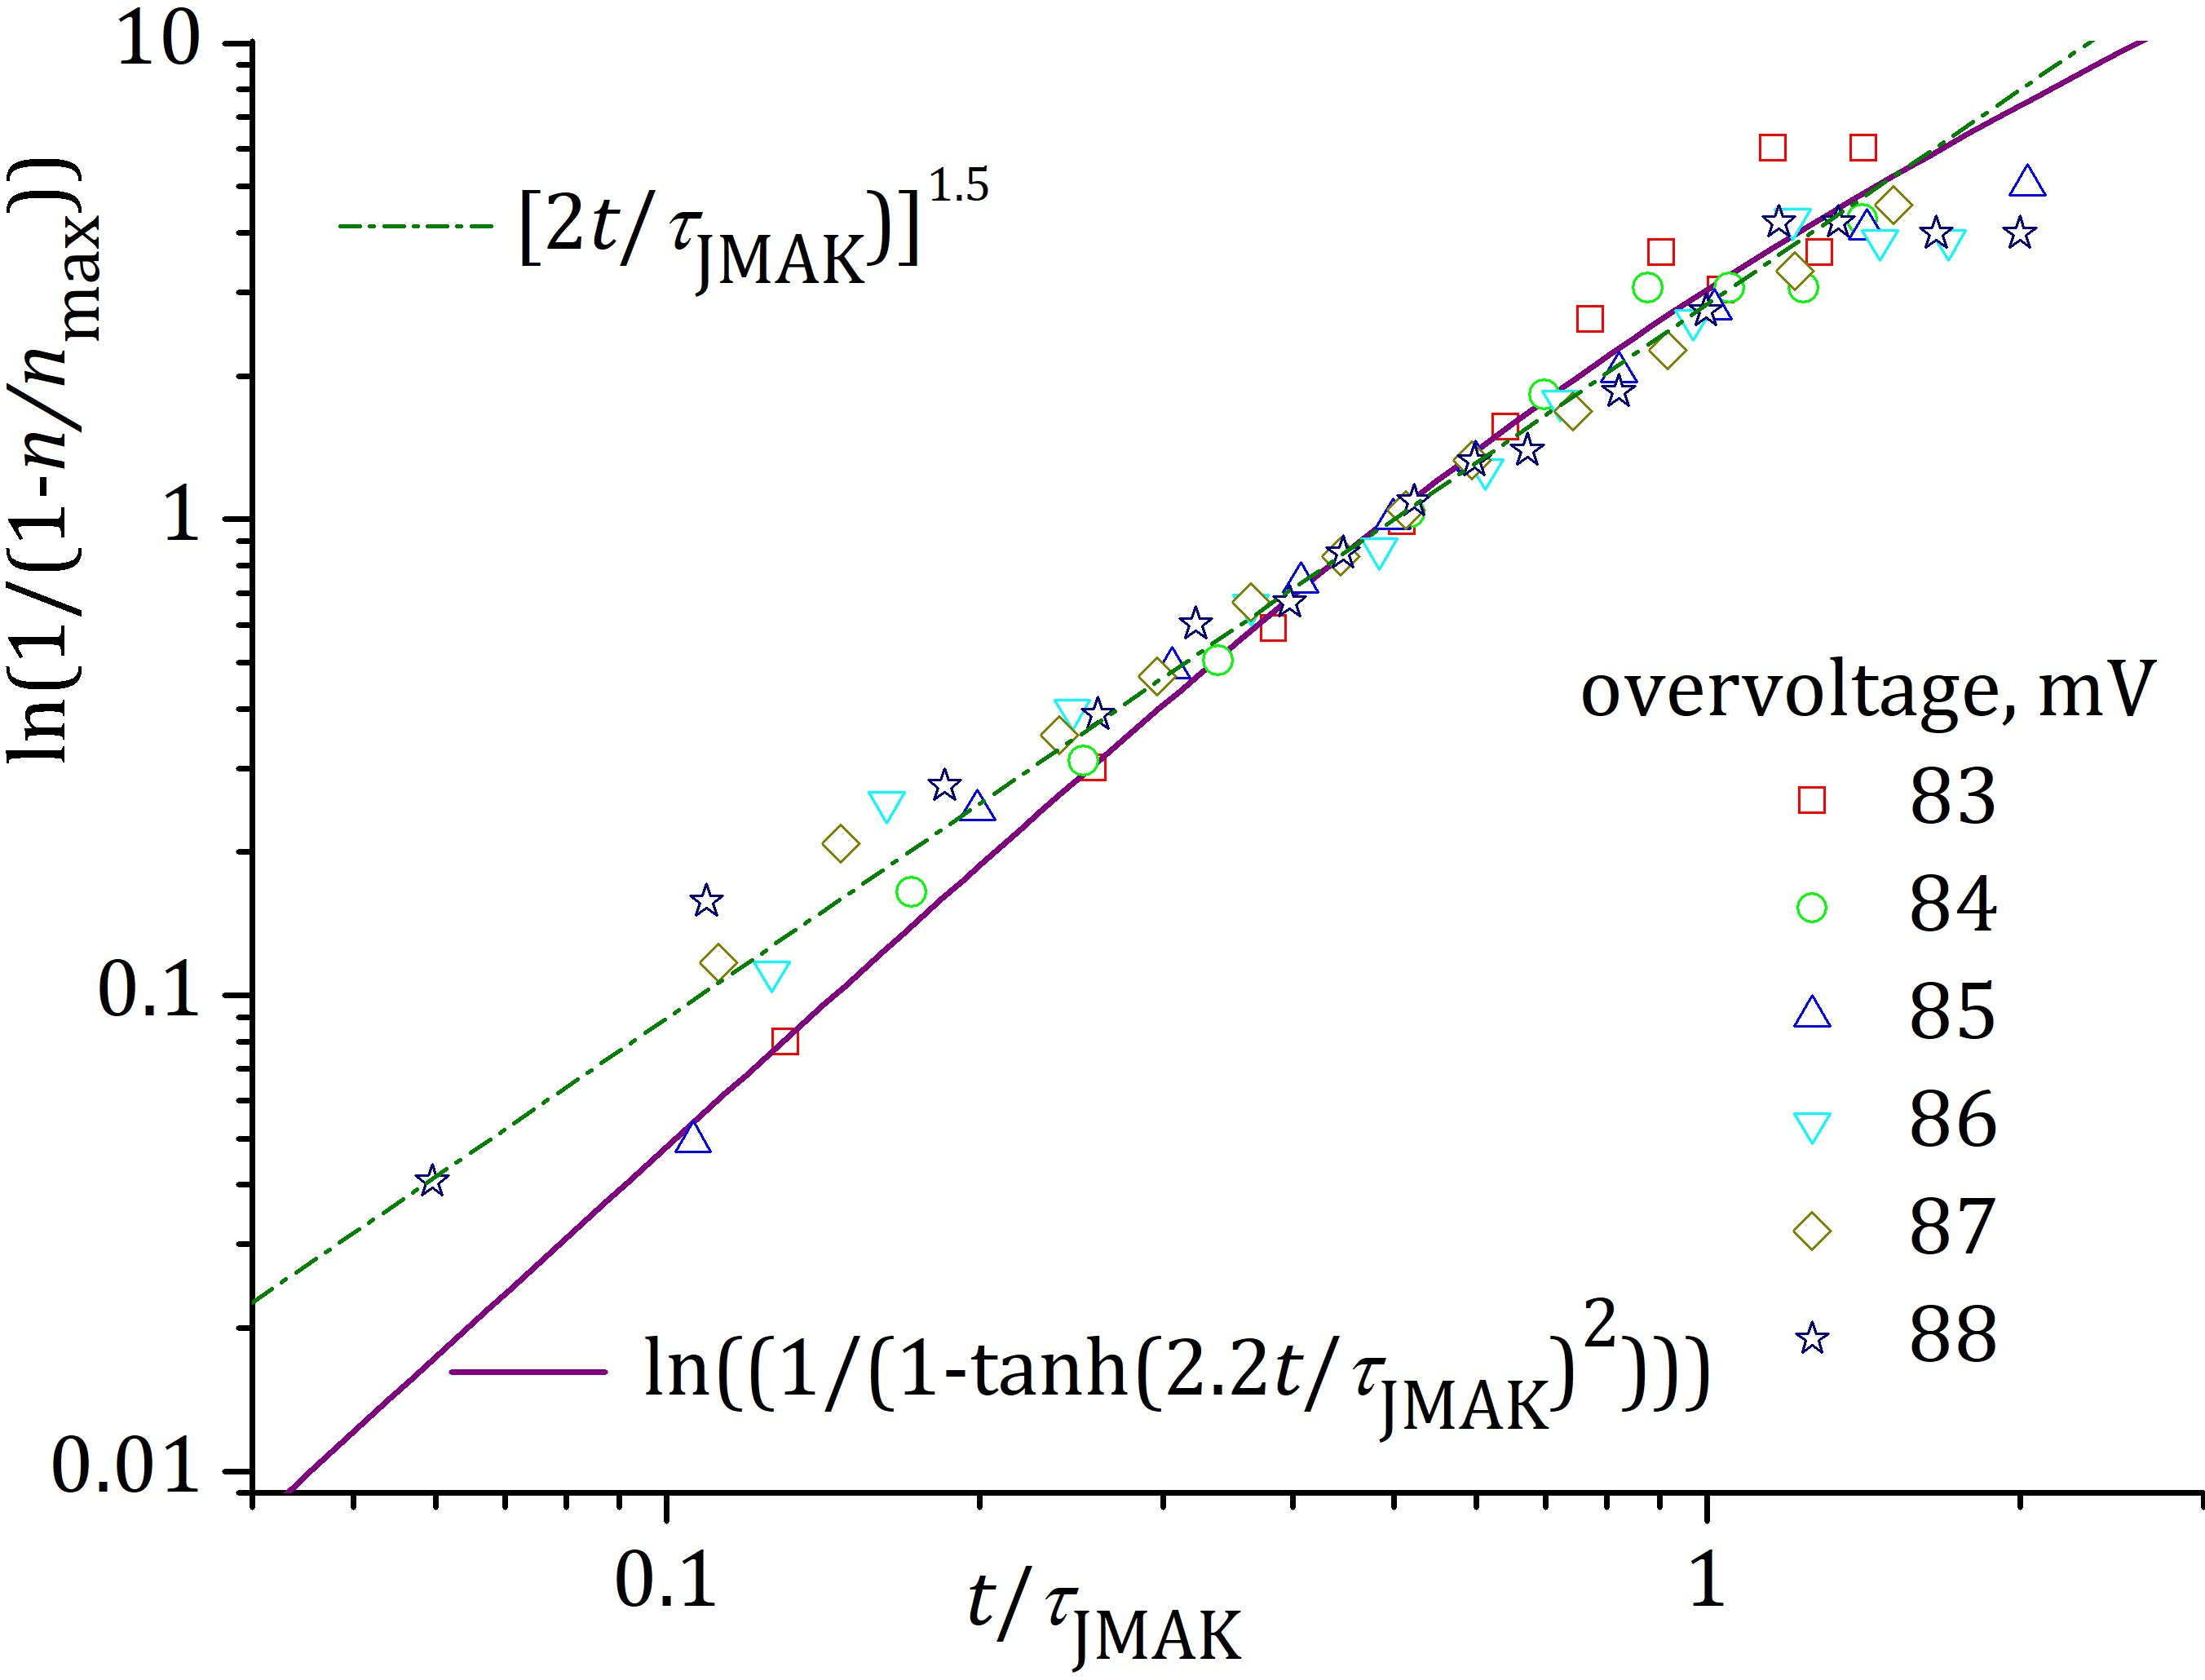
\includegraphics[width=0.48\textwidth]{ivan_markov_graphs/Fig6-jmak_rescaled_inAvramiCoordinates.jpg}}
    \caption{Рескалирани данни от JMAKn за различни свръхпотенциали в Аврами координати}
    \label{fig:jmakn_ivan_markov_avrami_plot}
\end{figure}
\autoref{fig:jmakn_ivan_markov_avrami_plot} представя много ясно основните слабости на JMAKn - несъответствието на модела на поведението на данните в Аврами координати за малки $\alpha$ и завоят за $\alpha \rightarrow 1$ спрямо $n$.

Липсата на универсална крива може да бъде пропуснато тук заради близките стойности на $n$, т.е. получените резултати за този параметър грубо да бъдат закръглени, но това ще доведе до съответно понижаване на $R^2$, тъй като моделът е нелинеен и чувствителен към промените на $n$.
\subsubsection{\texorpdfstring{$\alpha_{21}$}{α21}}
\begin{figure}[H]
    \centering
        \subfloat[Фиг. 5]{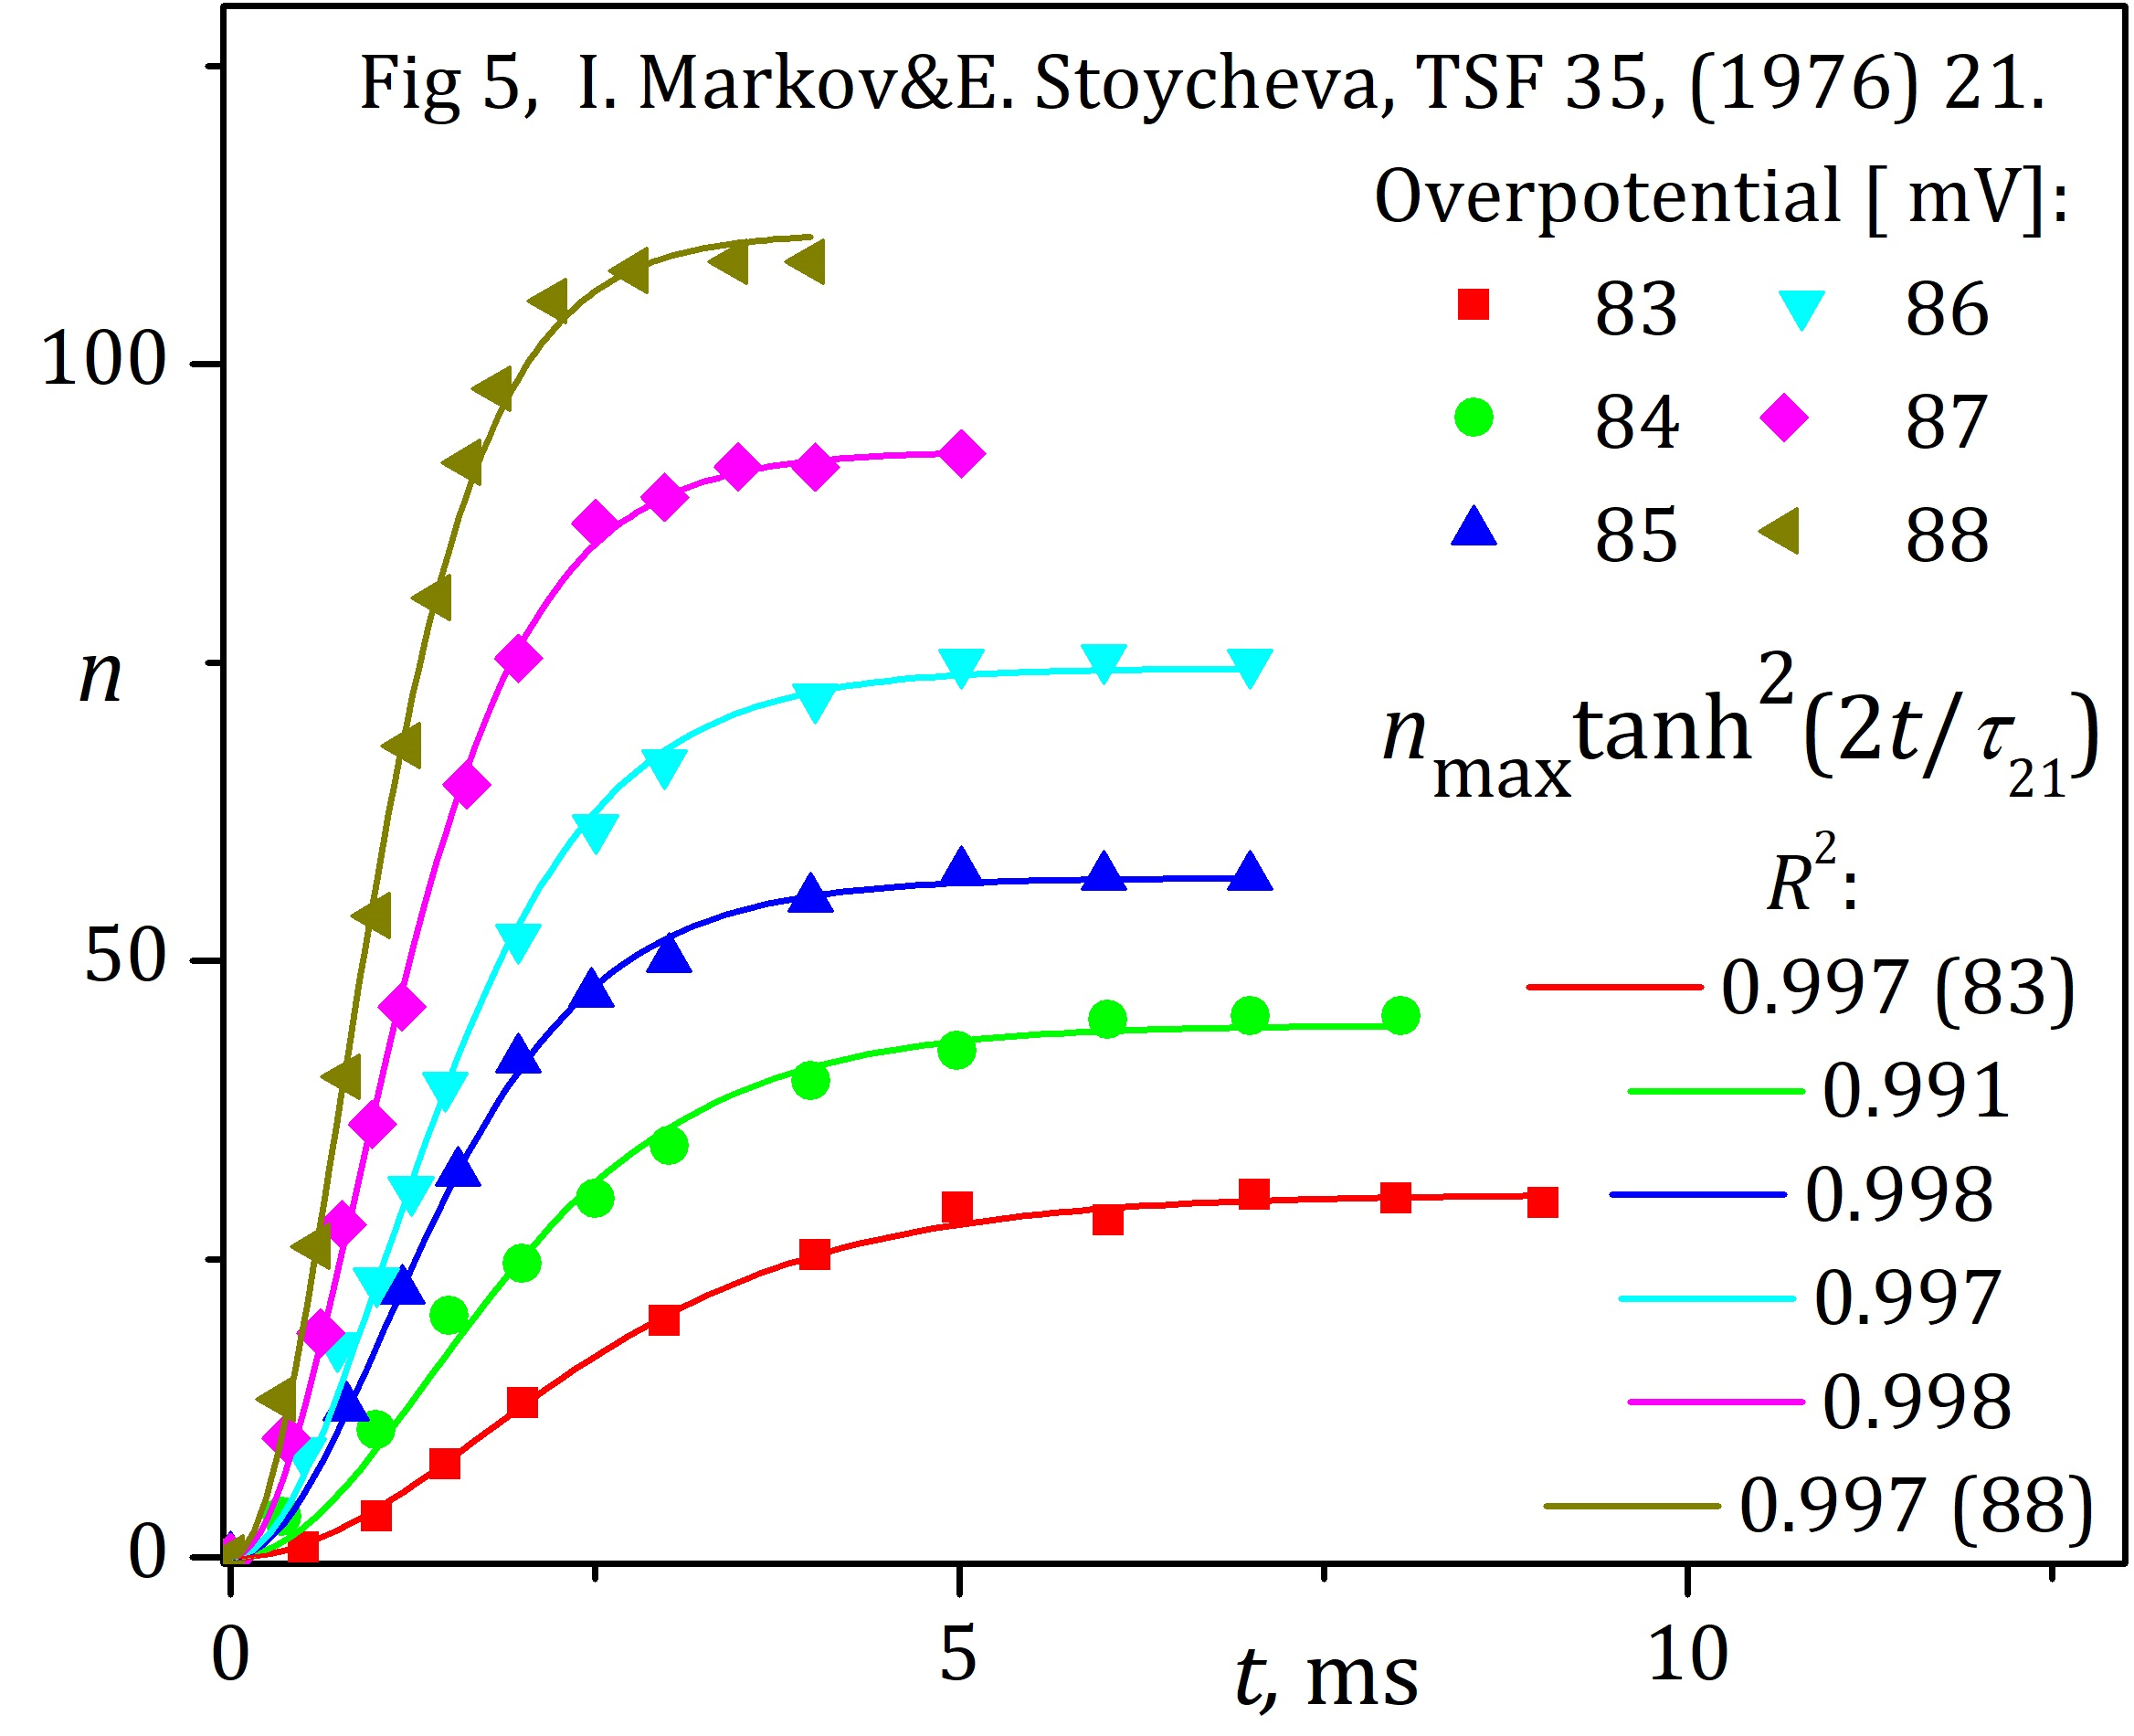
\includegraphics[width=0.48\textwidth]{ivan_markov_graphs/Fig5-alfa21-direct.jpg}}
        \subfloat[Фиг. 6]{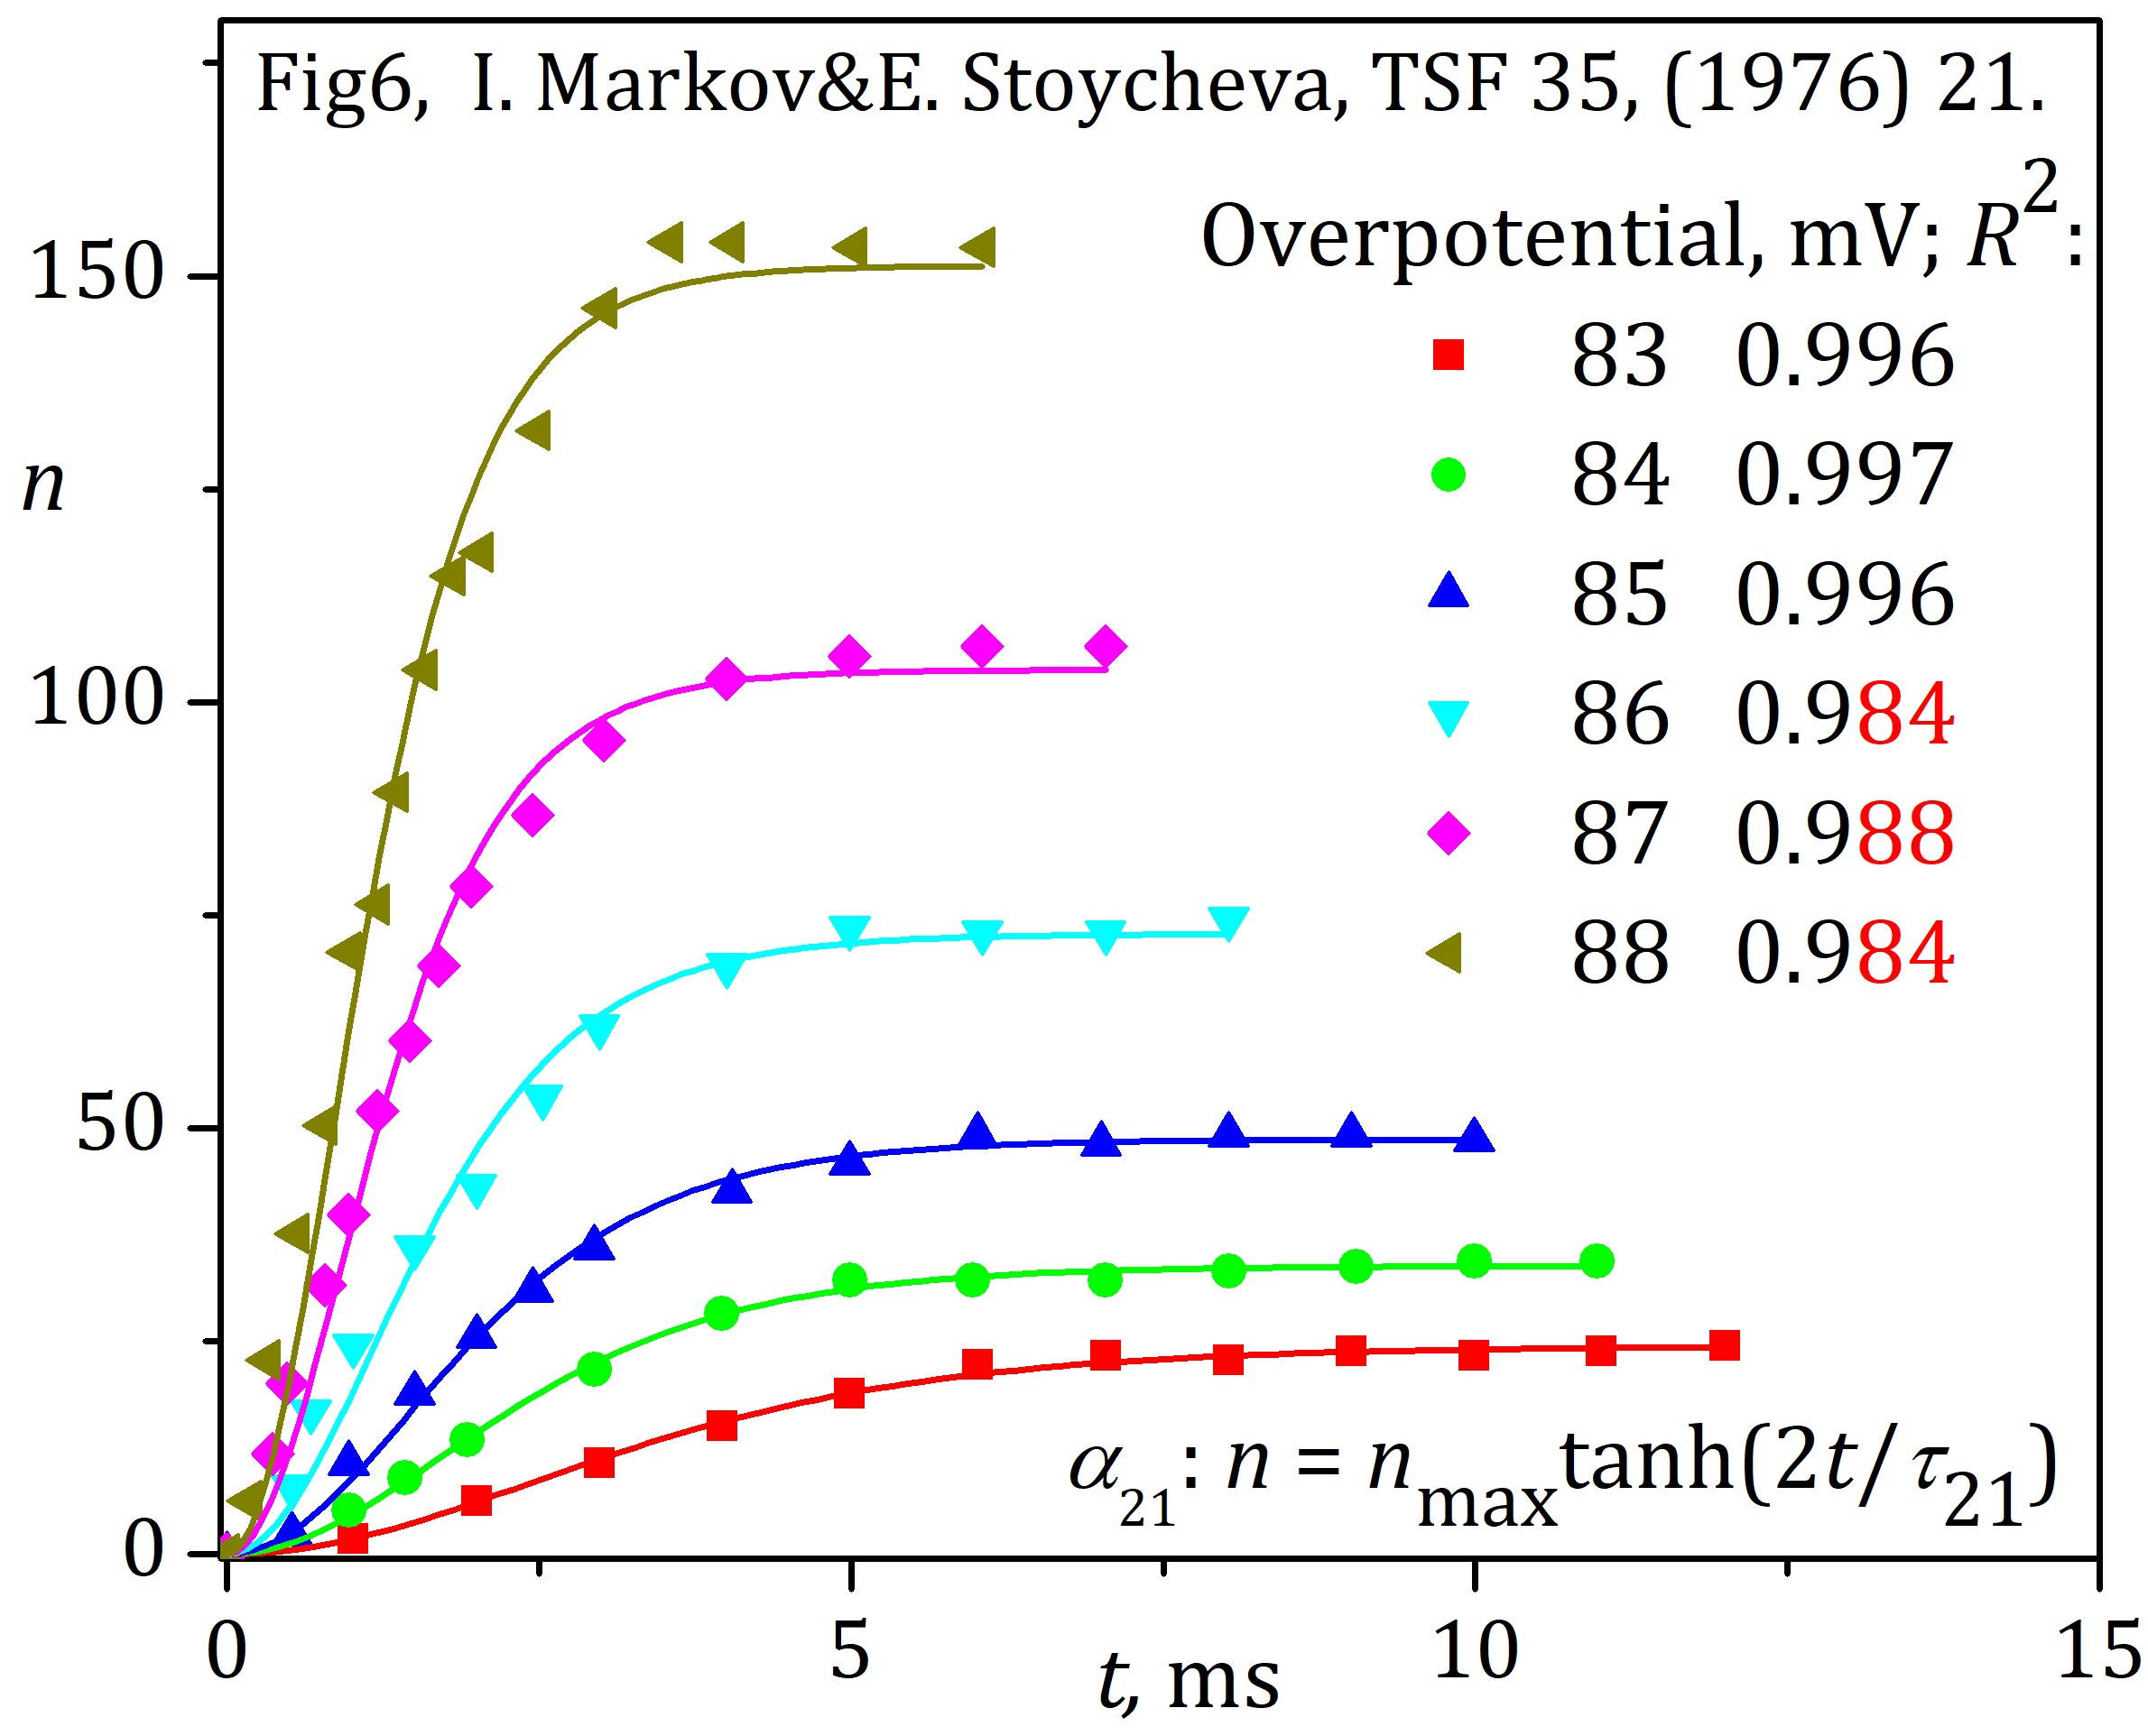
\includegraphics[width=0.48\textwidth]{ivan_markov_graphs/Fig6_alfa21-direct.jpg}}
    \caption{Данни от \cite{Markov1976} и съответните криви за $\alpha_{21}$ и съответни стойности за $R^2$}
\end{figure}

Тъй като имаме единствен параметър ($\tau_{21}$) освен $N_{max}$, можем да представим всички данни на универсална крива. Това е и основно достойнство на изведения от нас модел.

\begin{figure}[H]
    \centering
        \subfloat[Фиг. 5]{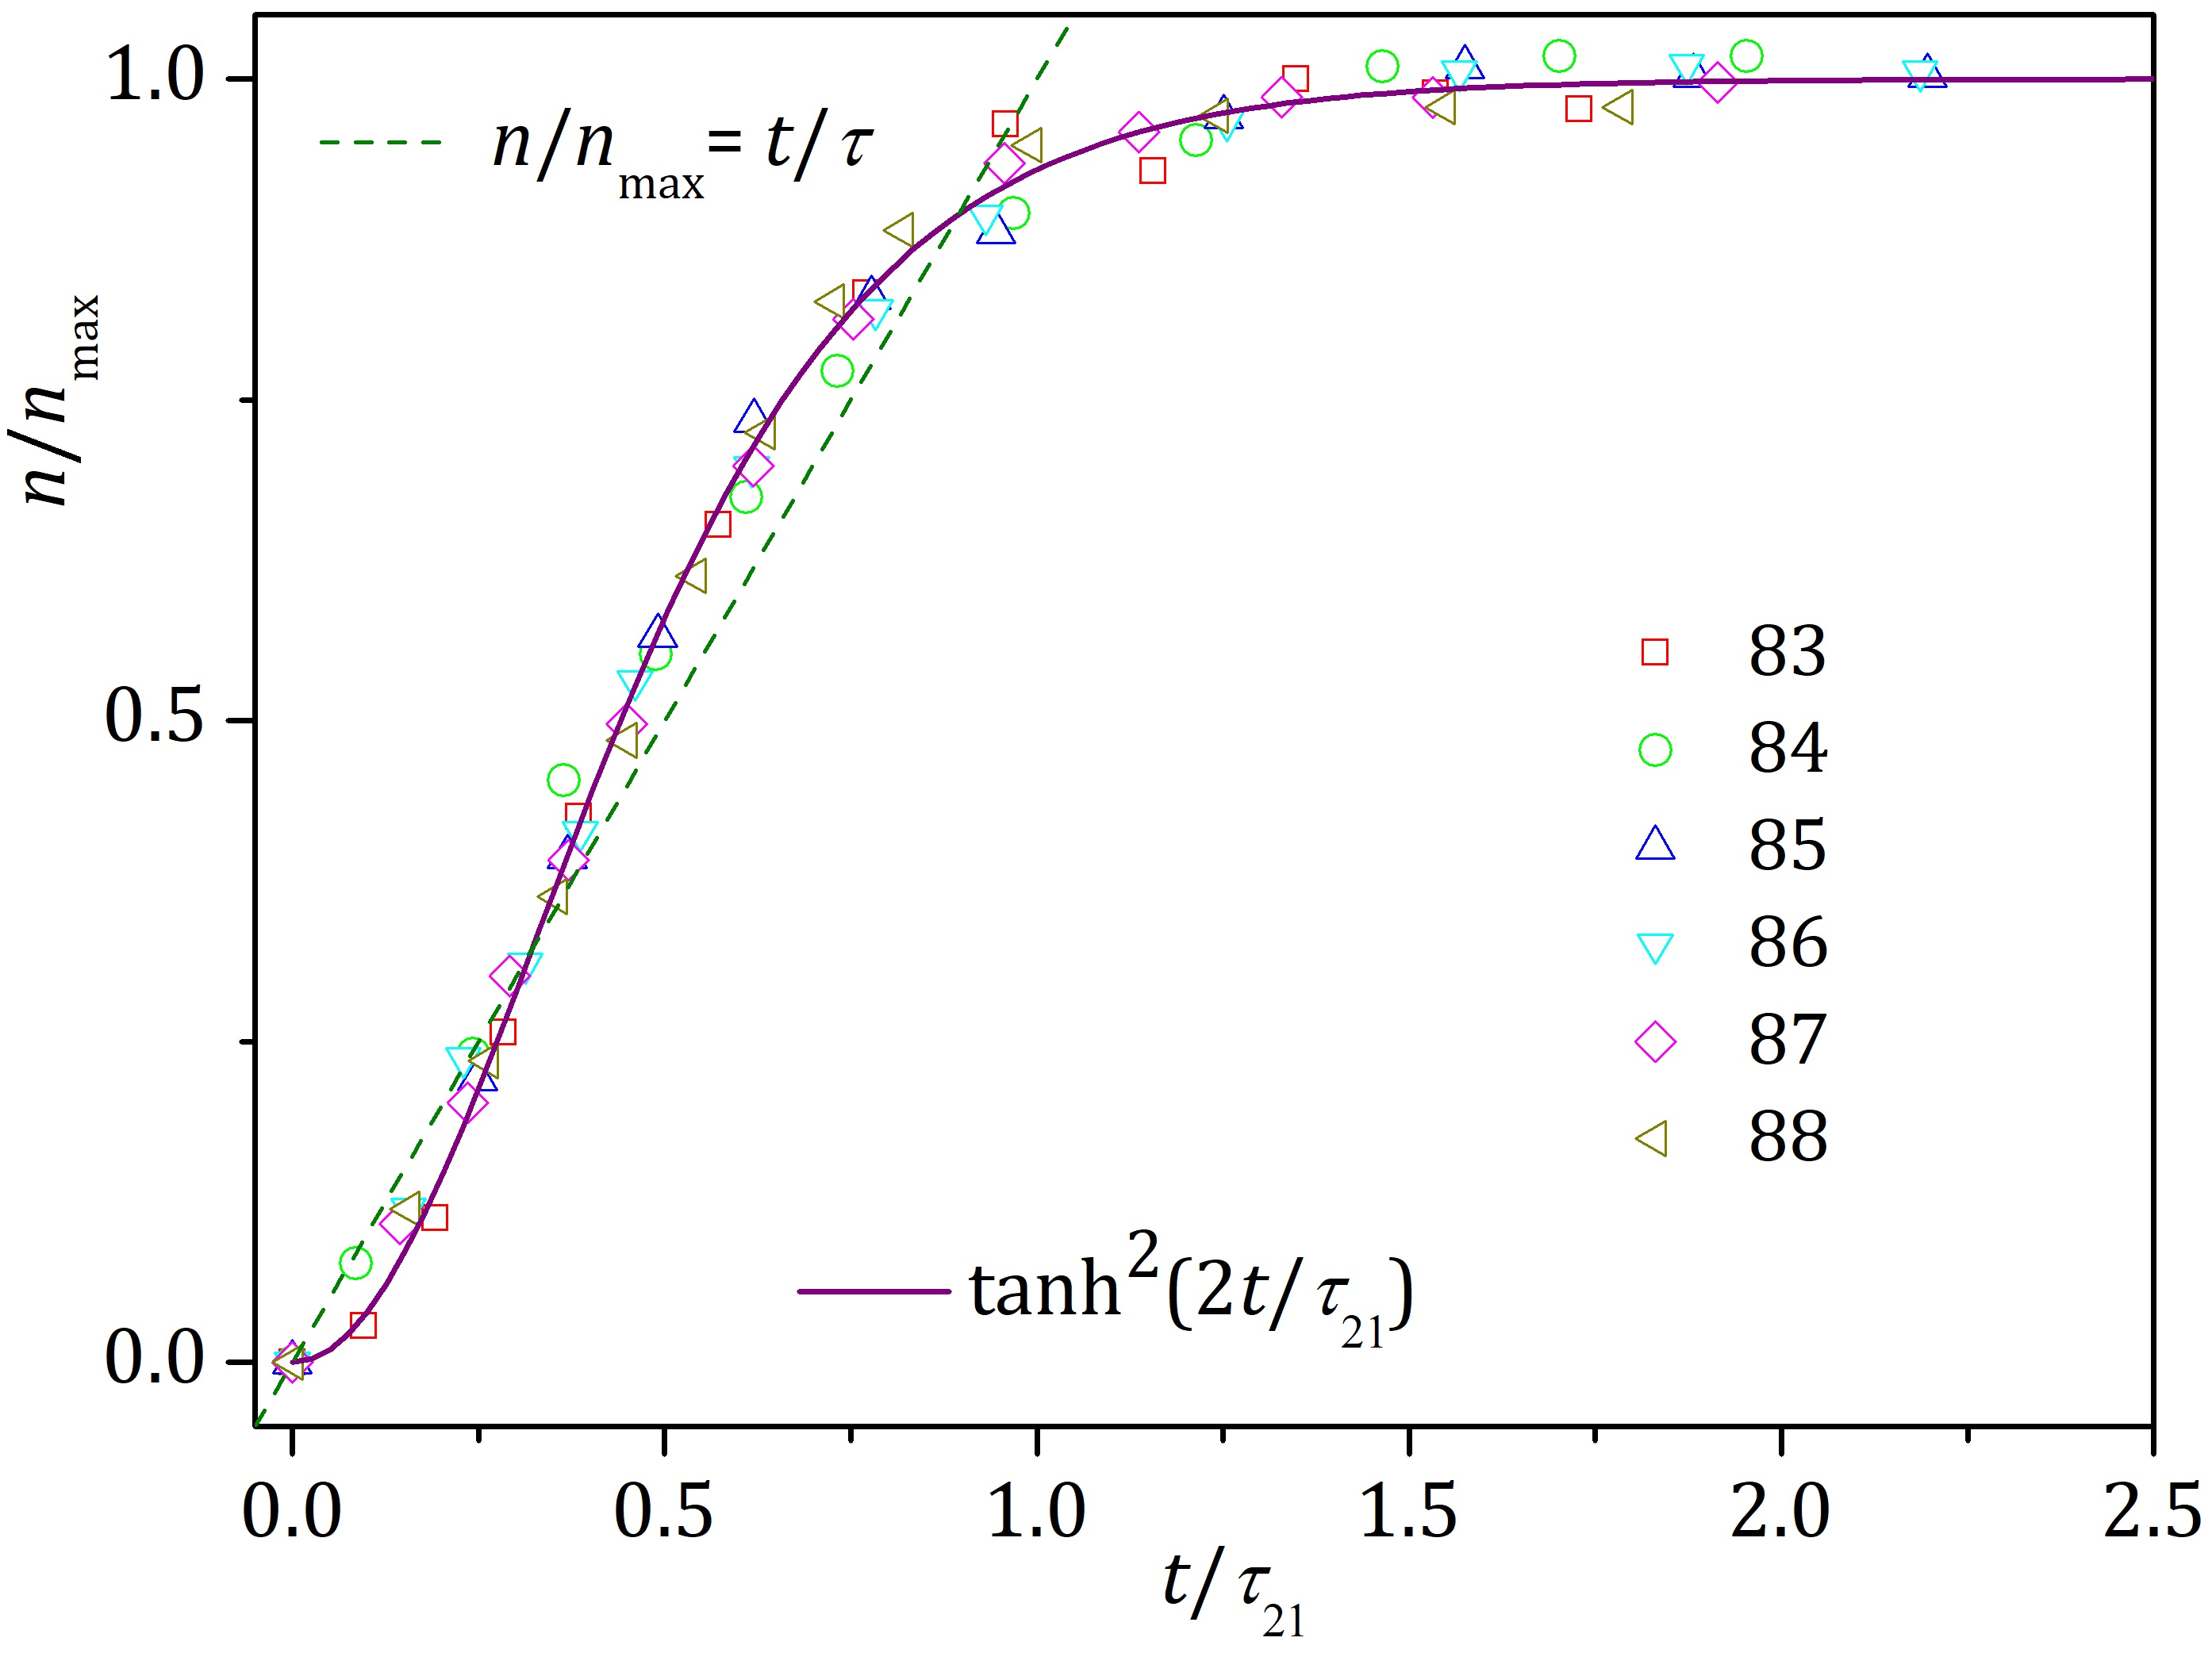
\includegraphics[width=0.48\textwidth]{ivan_markov_graphs/Fig5-alfa21_rescaled.jpg}}
        \subfloat[Фиг. 6]{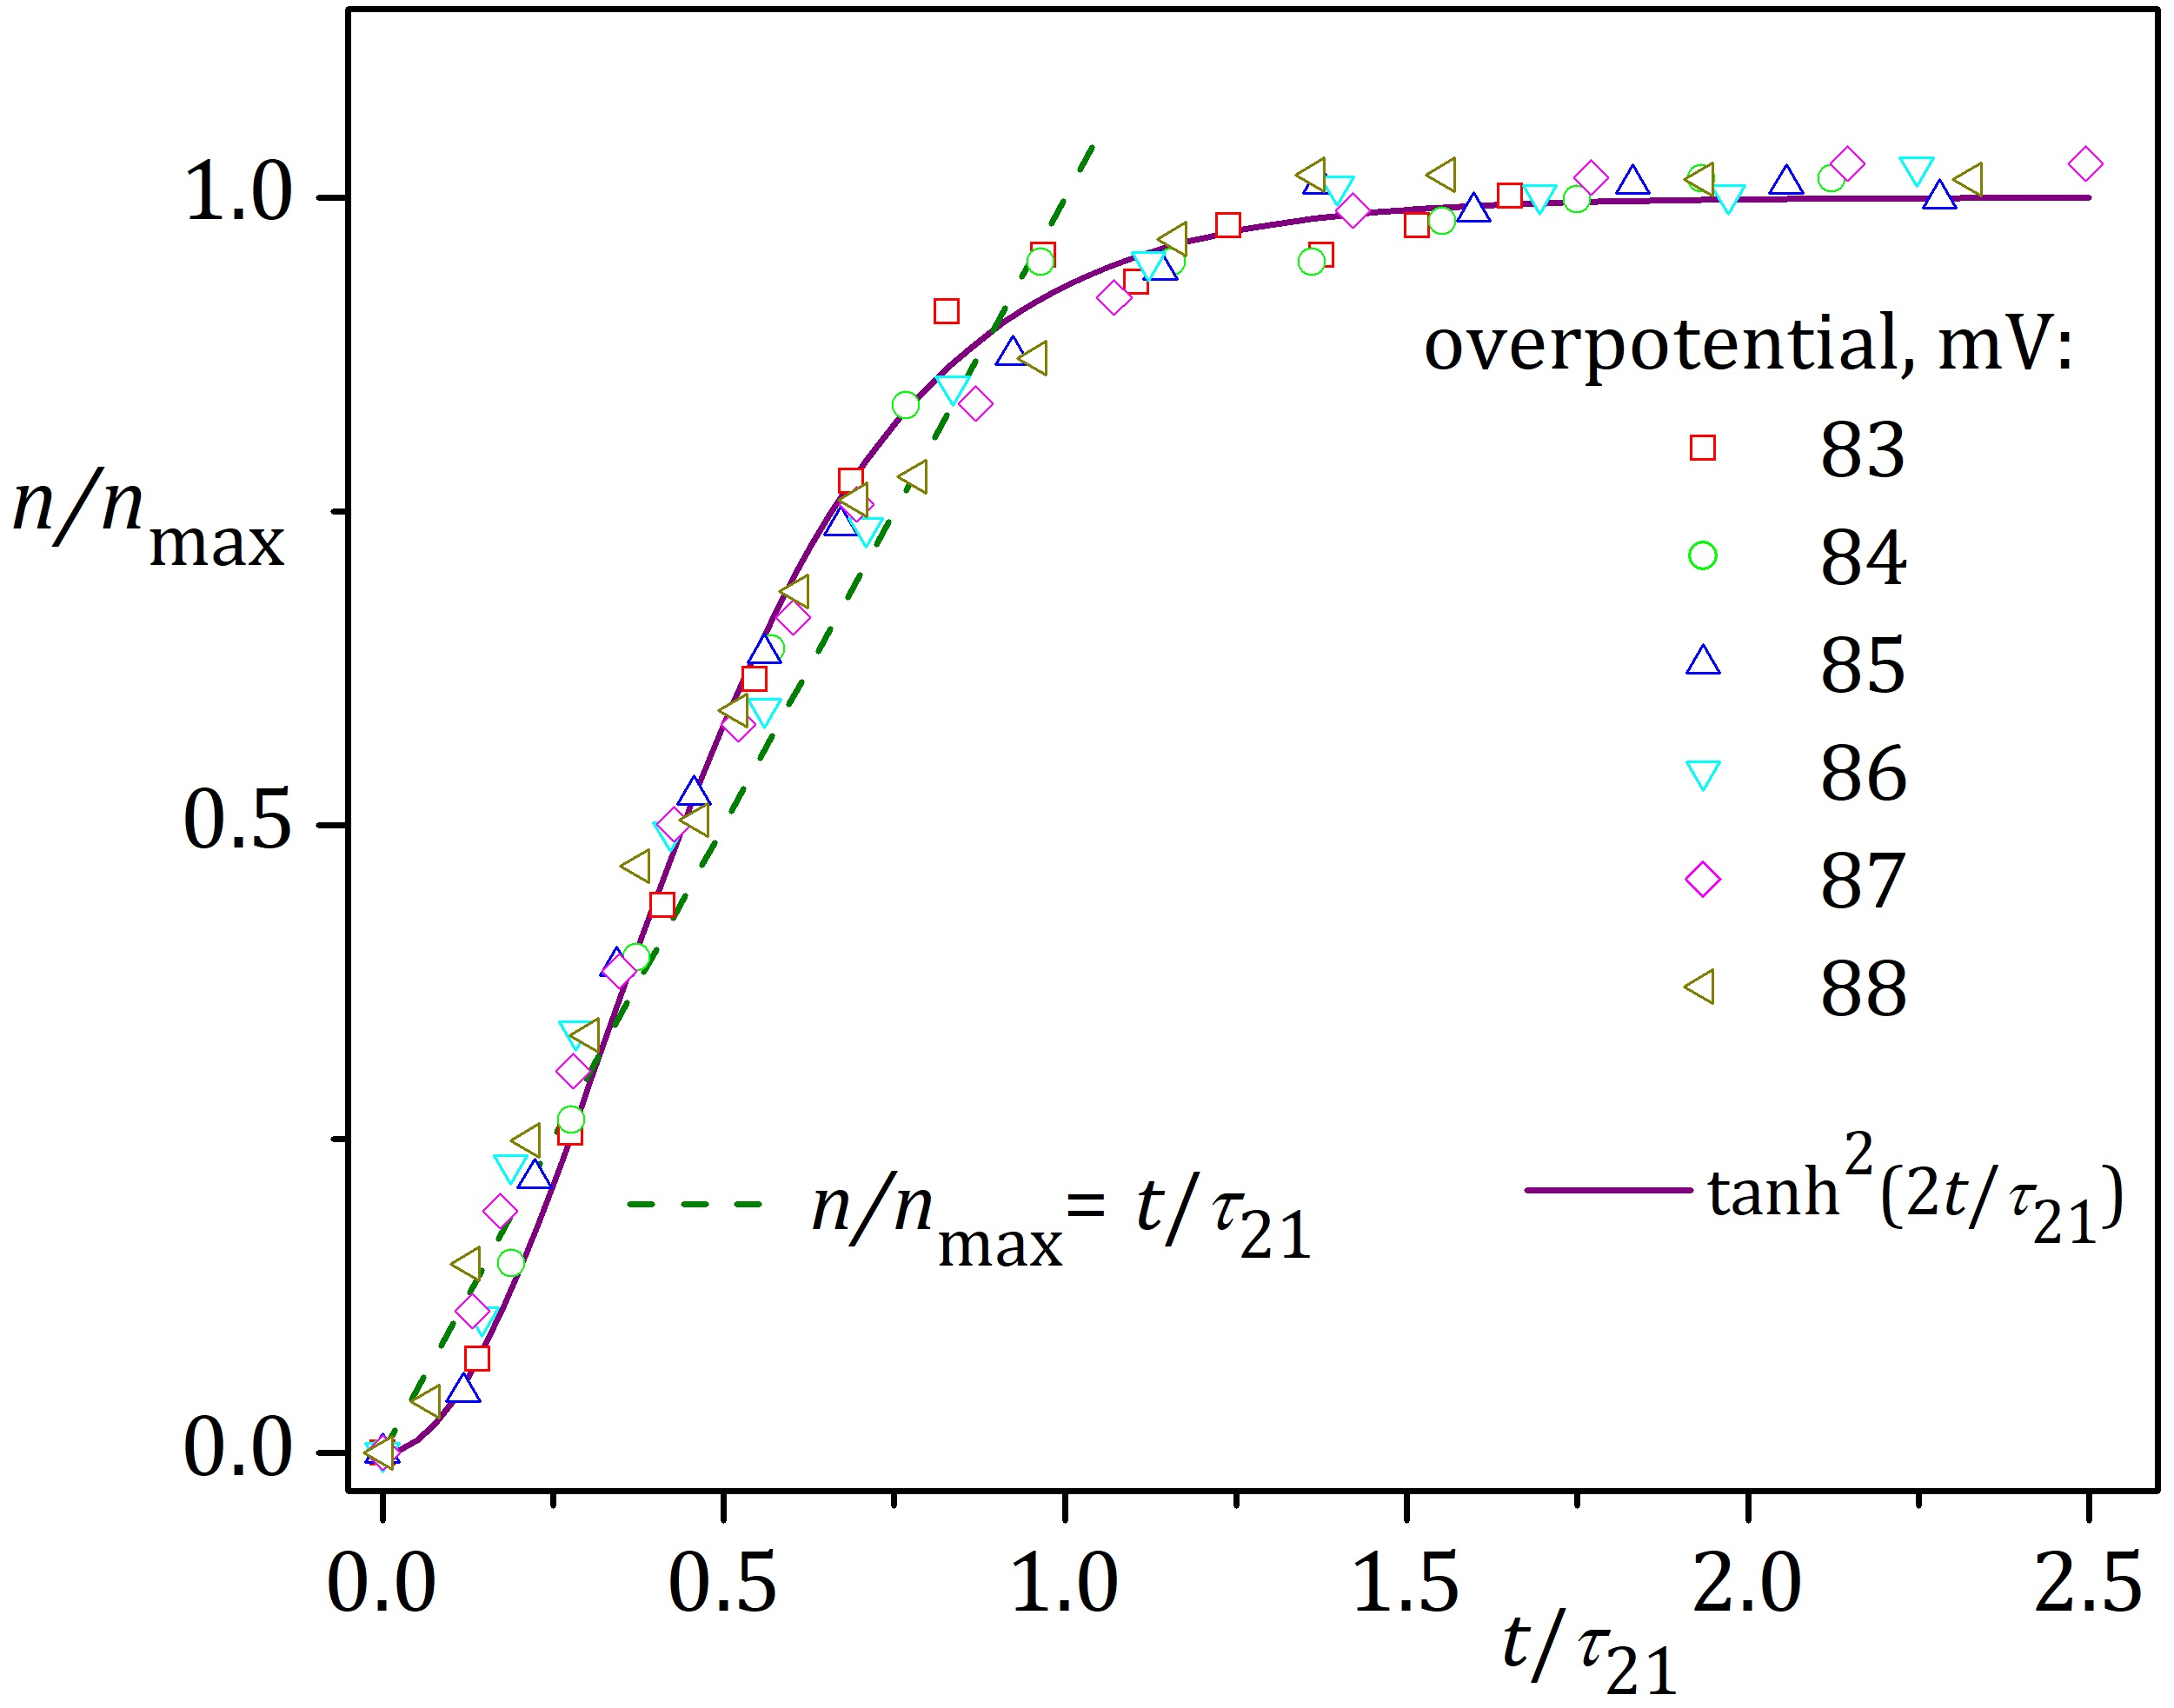
\includegraphics[width=0.48\textwidth]{ivan_markov_graphs/Fig6_alfa21_rescaled.jpg}}
    \caption{Рескалирани данни от \cite{Markov1976} и универсалната крива за $\alpha_{21}$}
    \label{fig:alfa21_ivan_markov_master_curve}
\end{figure}
\autoref{fig:alfa21_ivan_markov_master_curve} представя апотеоза на нашите разглеждания до тук - от чисто физичните съображения (потвърдени с резултатите за $n$ от JMAKn) избрахме $\aDg$ аналитична крива. За различните експериментални условия определихме $N_{max}$ и $\tau$. Тези параметри използваме след това, за да рескалираме експерименталинте данни. Така получаваме универсално поведение, което не може да бъде разкрито с моделите с повече параметри.
\begin{figure}[H]
    \centering
        \subfloat[Фиг. 5]{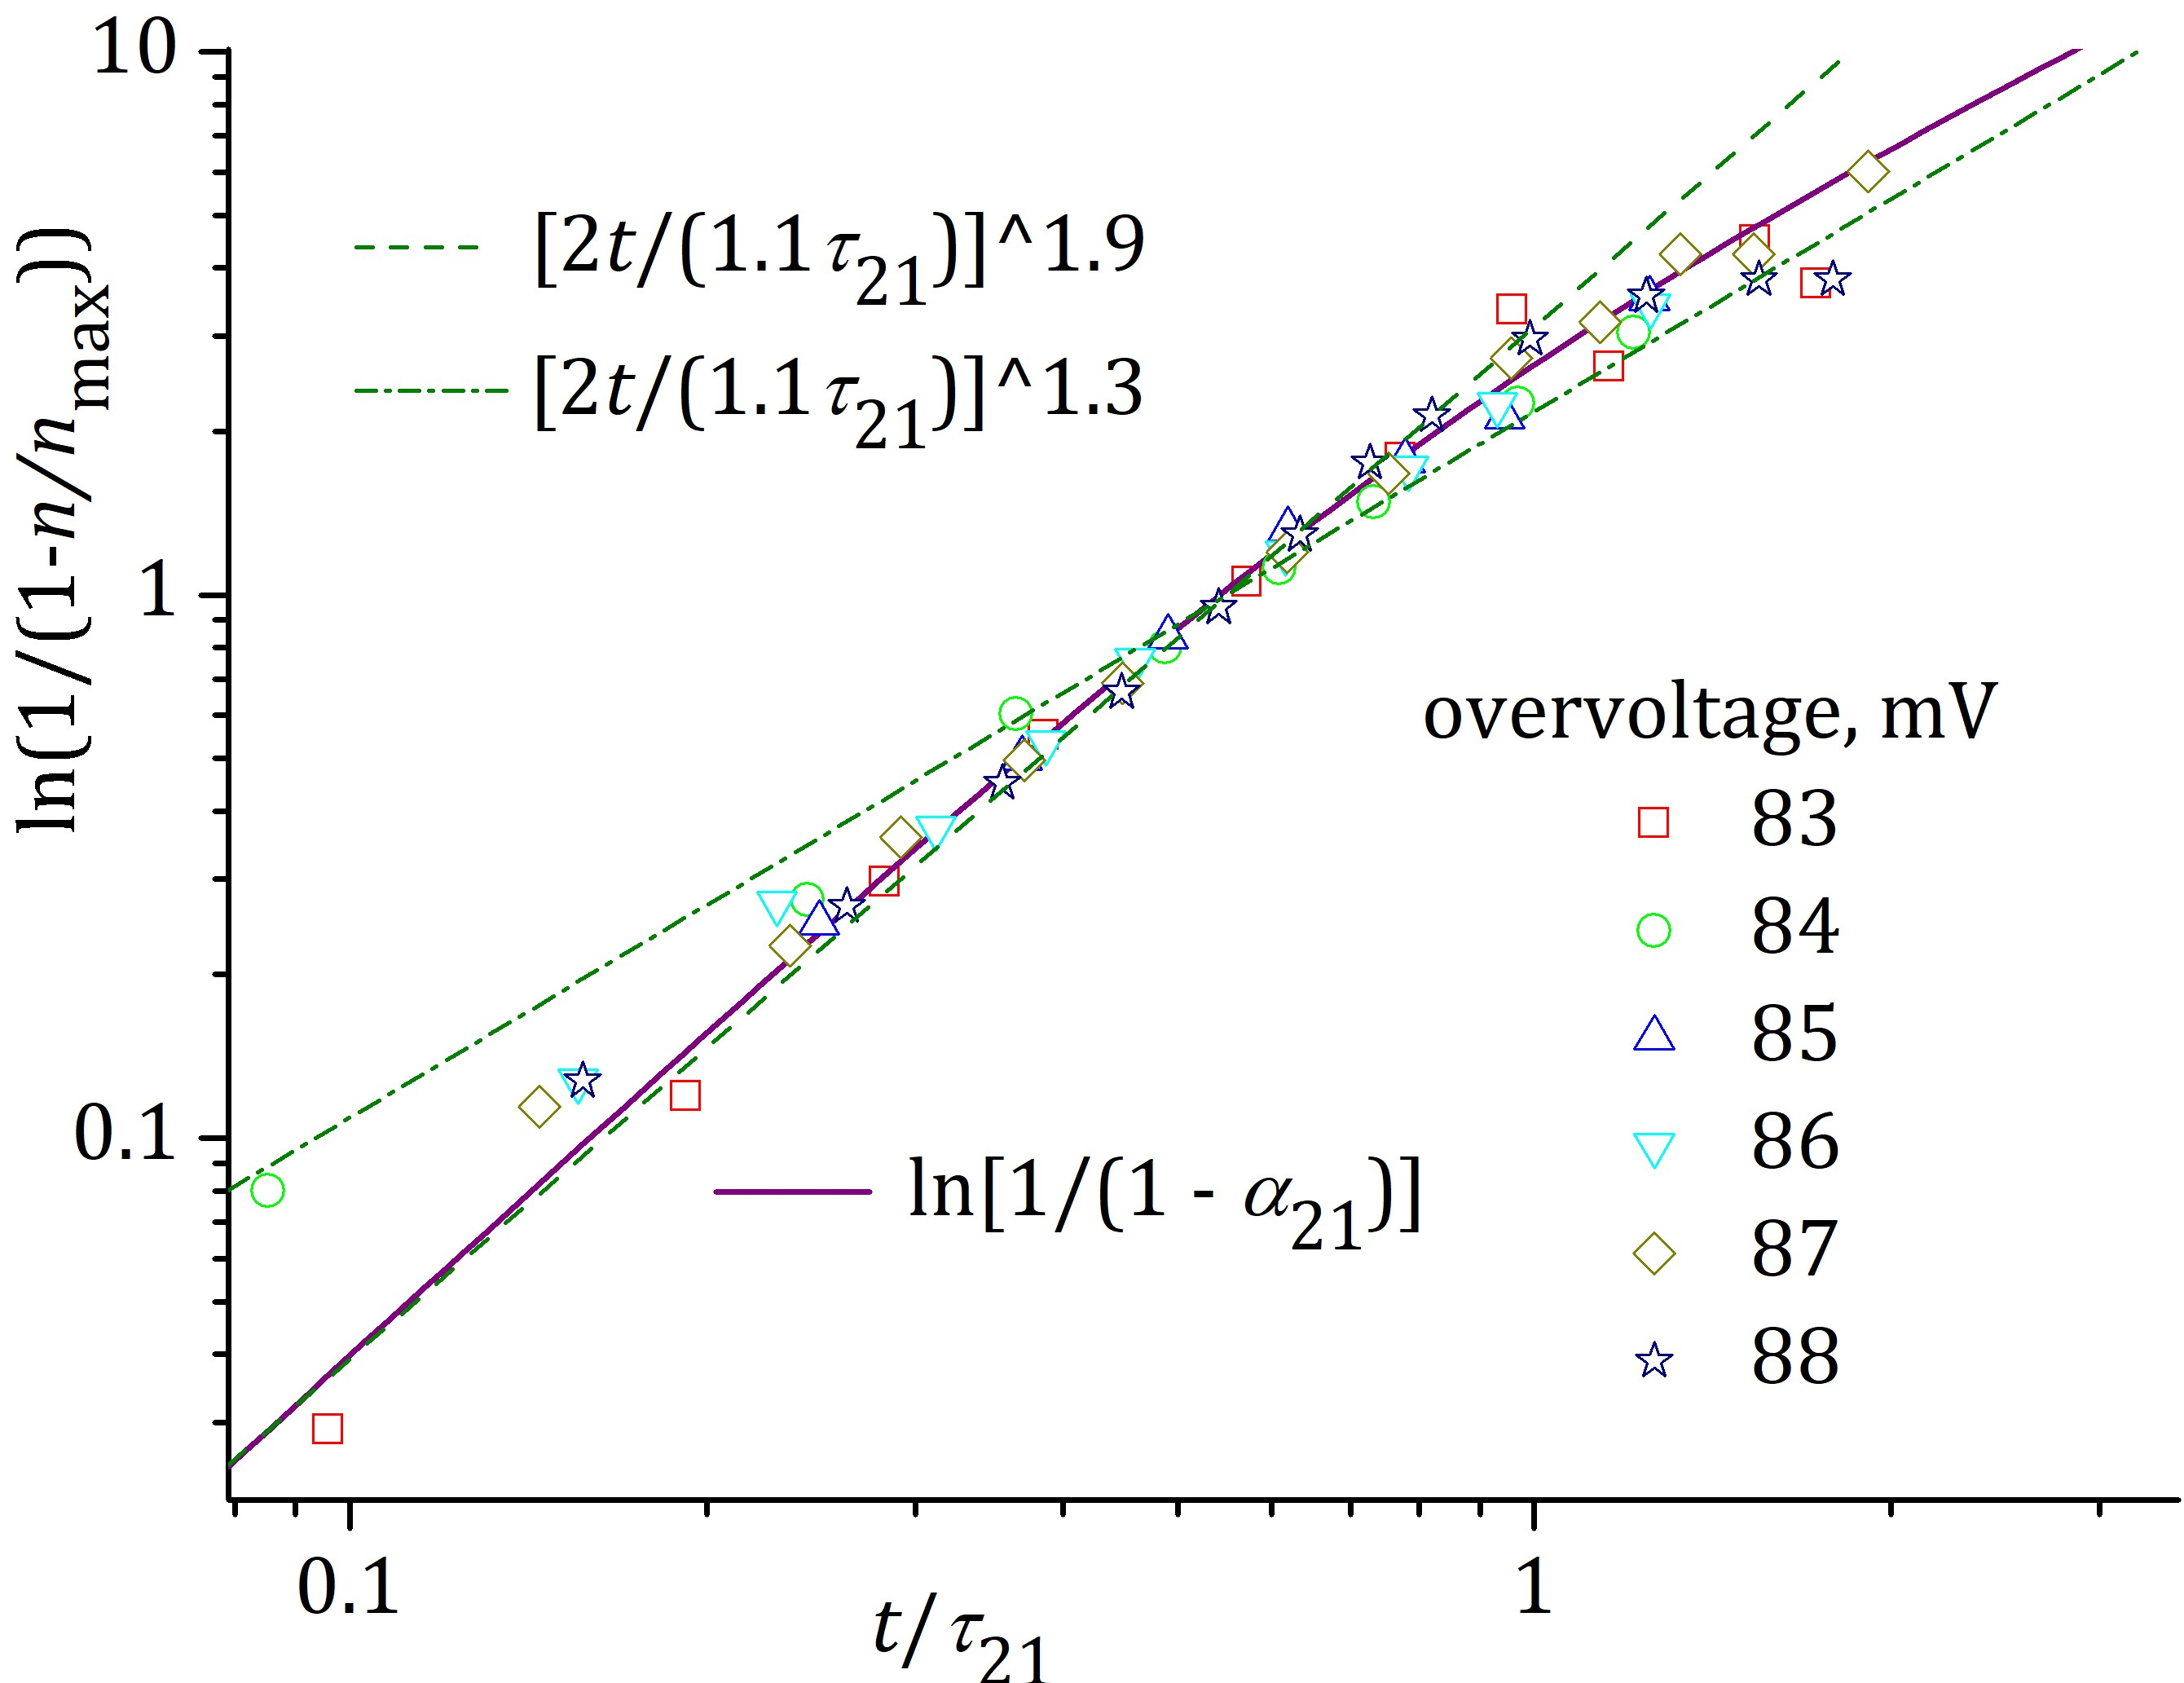
\includegraphics[width=0.48\textwidth]{ivan_markov_graphs/Fig5-alfa21-avrami-plot.jpg}}
        \subfloat[Фиг. 6]{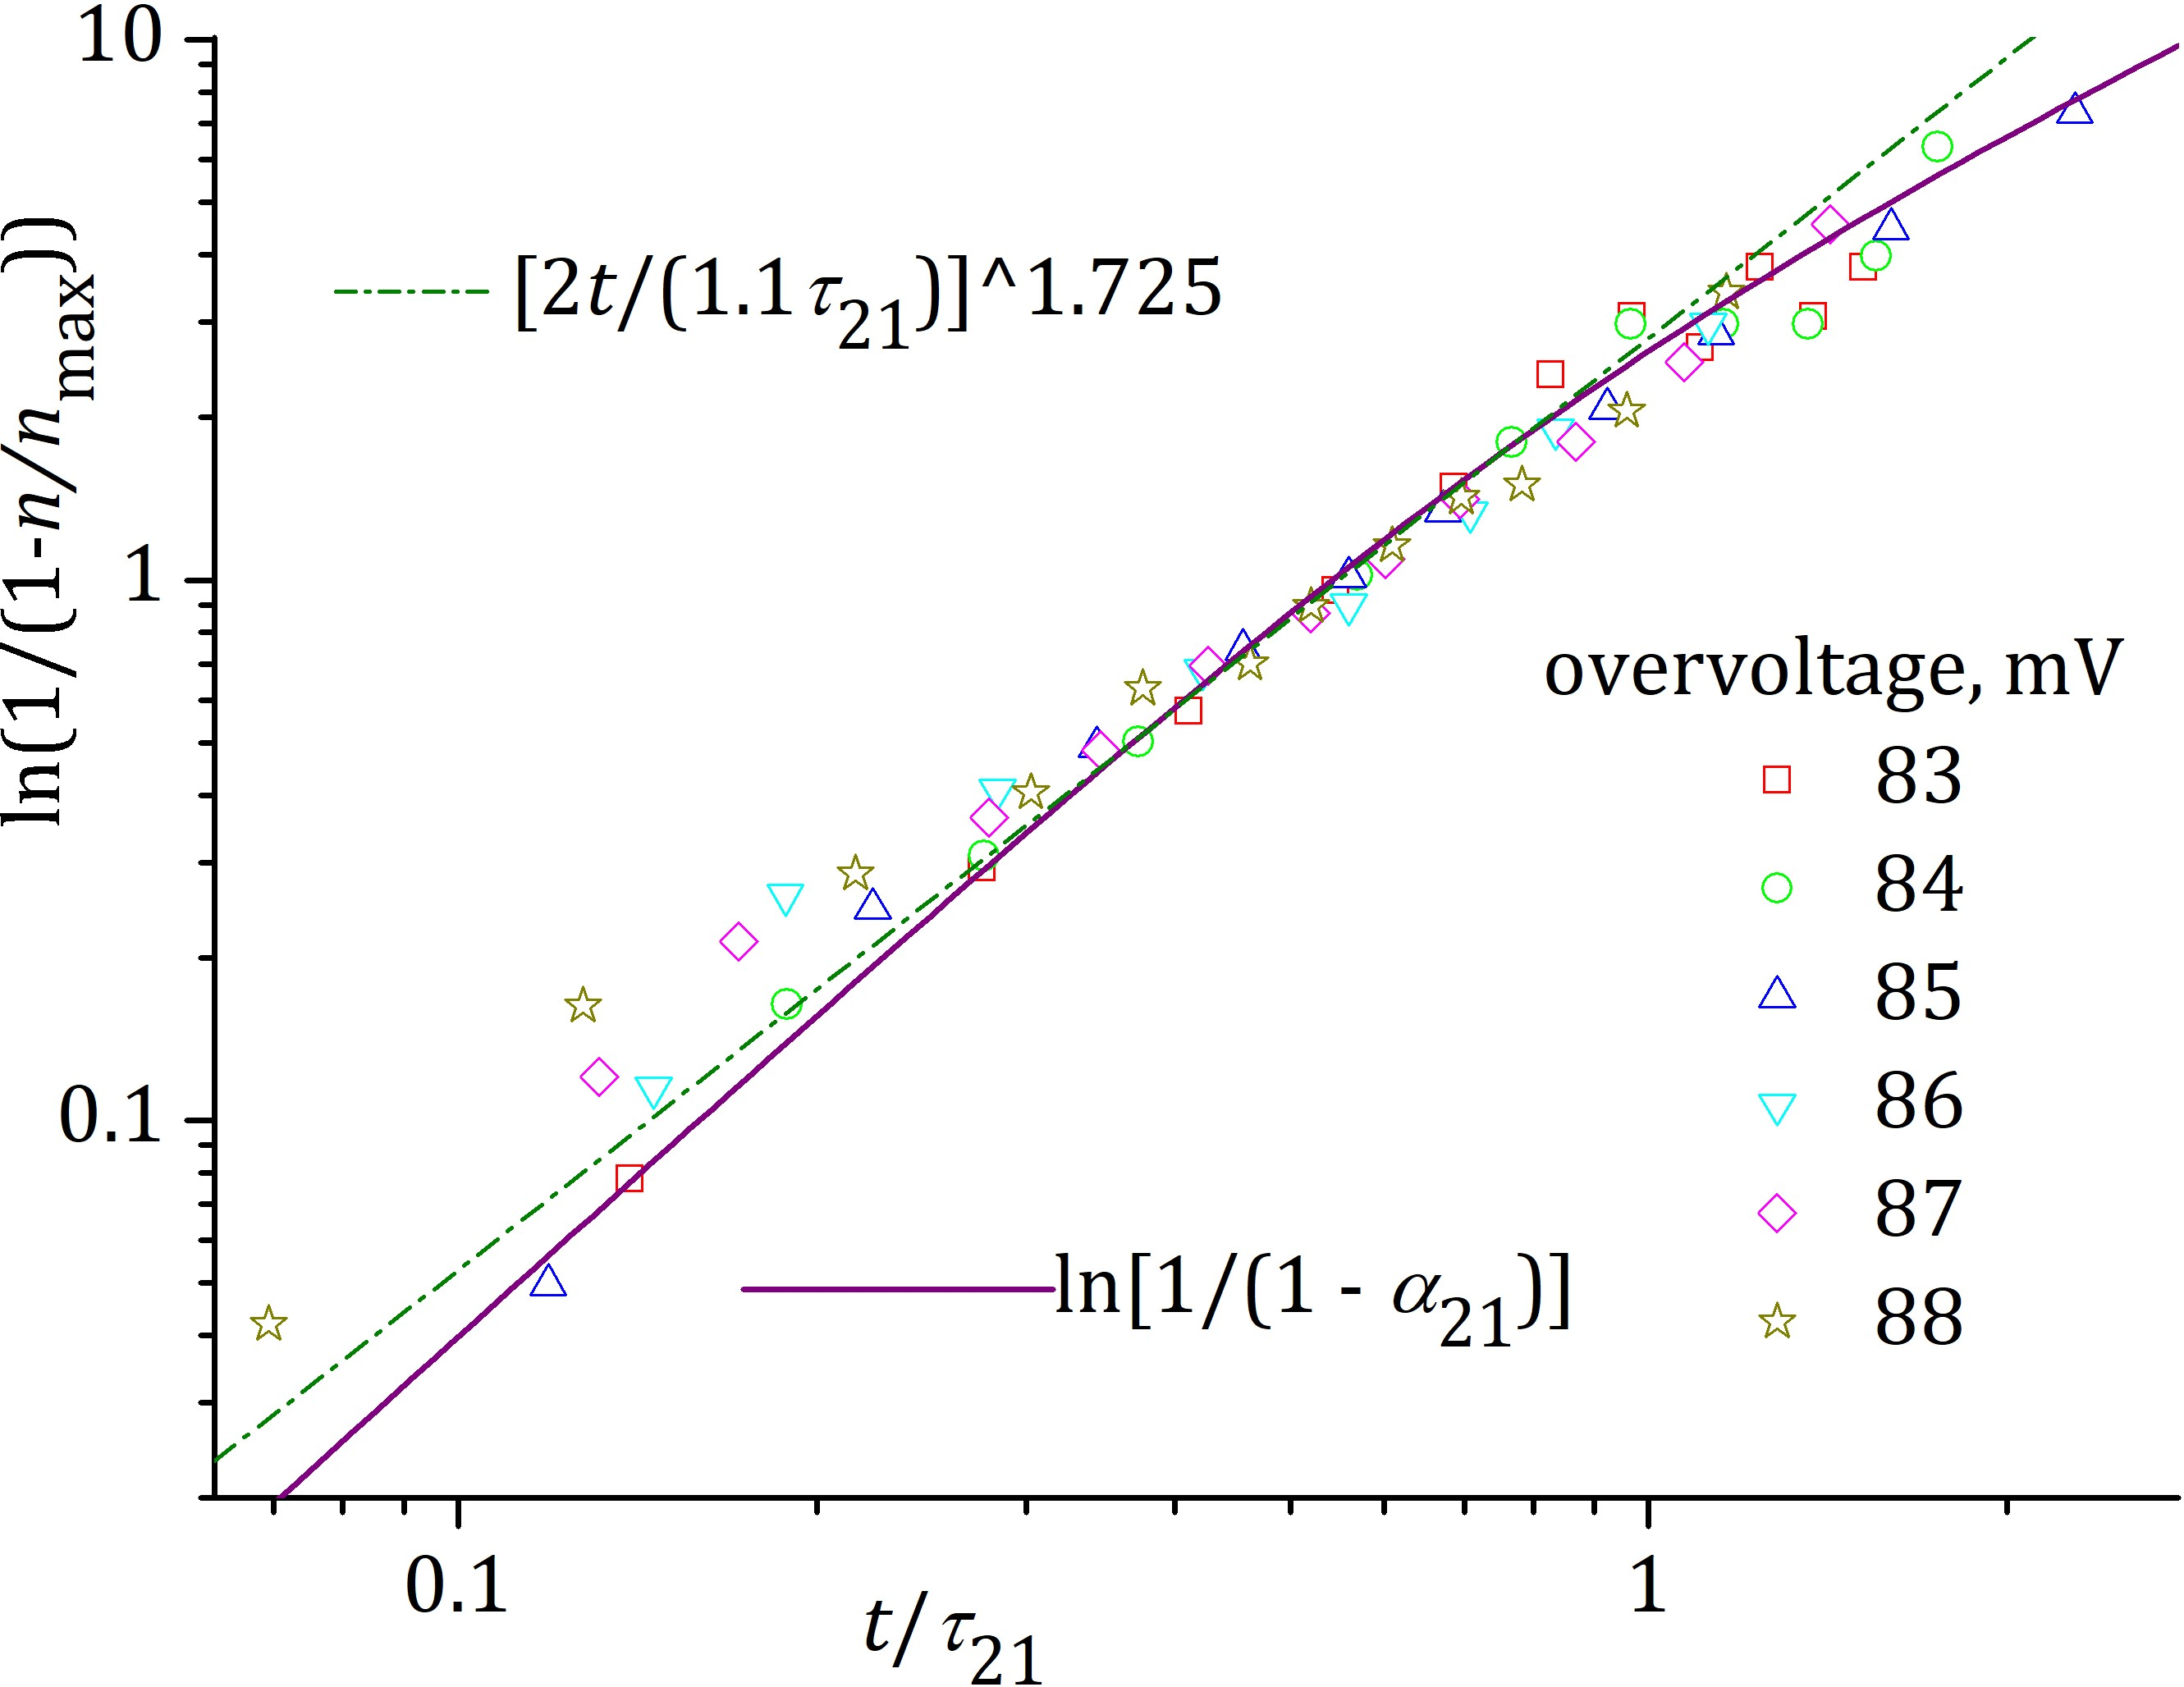
\includegraphics[width=0.48\textwidth]{ivan_markov_graphs/Fig6-alfa21-avrami-plot.jpg}}
    \caption{Рескалирани данни от \cite{Markov1976} и универсалната крива за $\alpha_{21}$ в Аврами координати. Показани са криви и за различни $n$ от JMAKn. Завоят на данните за $\alpha \rightarrow 1$ е очевиден.}
    \label{fig:alfa21_ivan_markov_master_curve_avrami}
\end{figure}
\begin{figure}[H]
    \centering
        \subfloat[Фиг. 5\label{subfig:alfa21_params_fig5}]{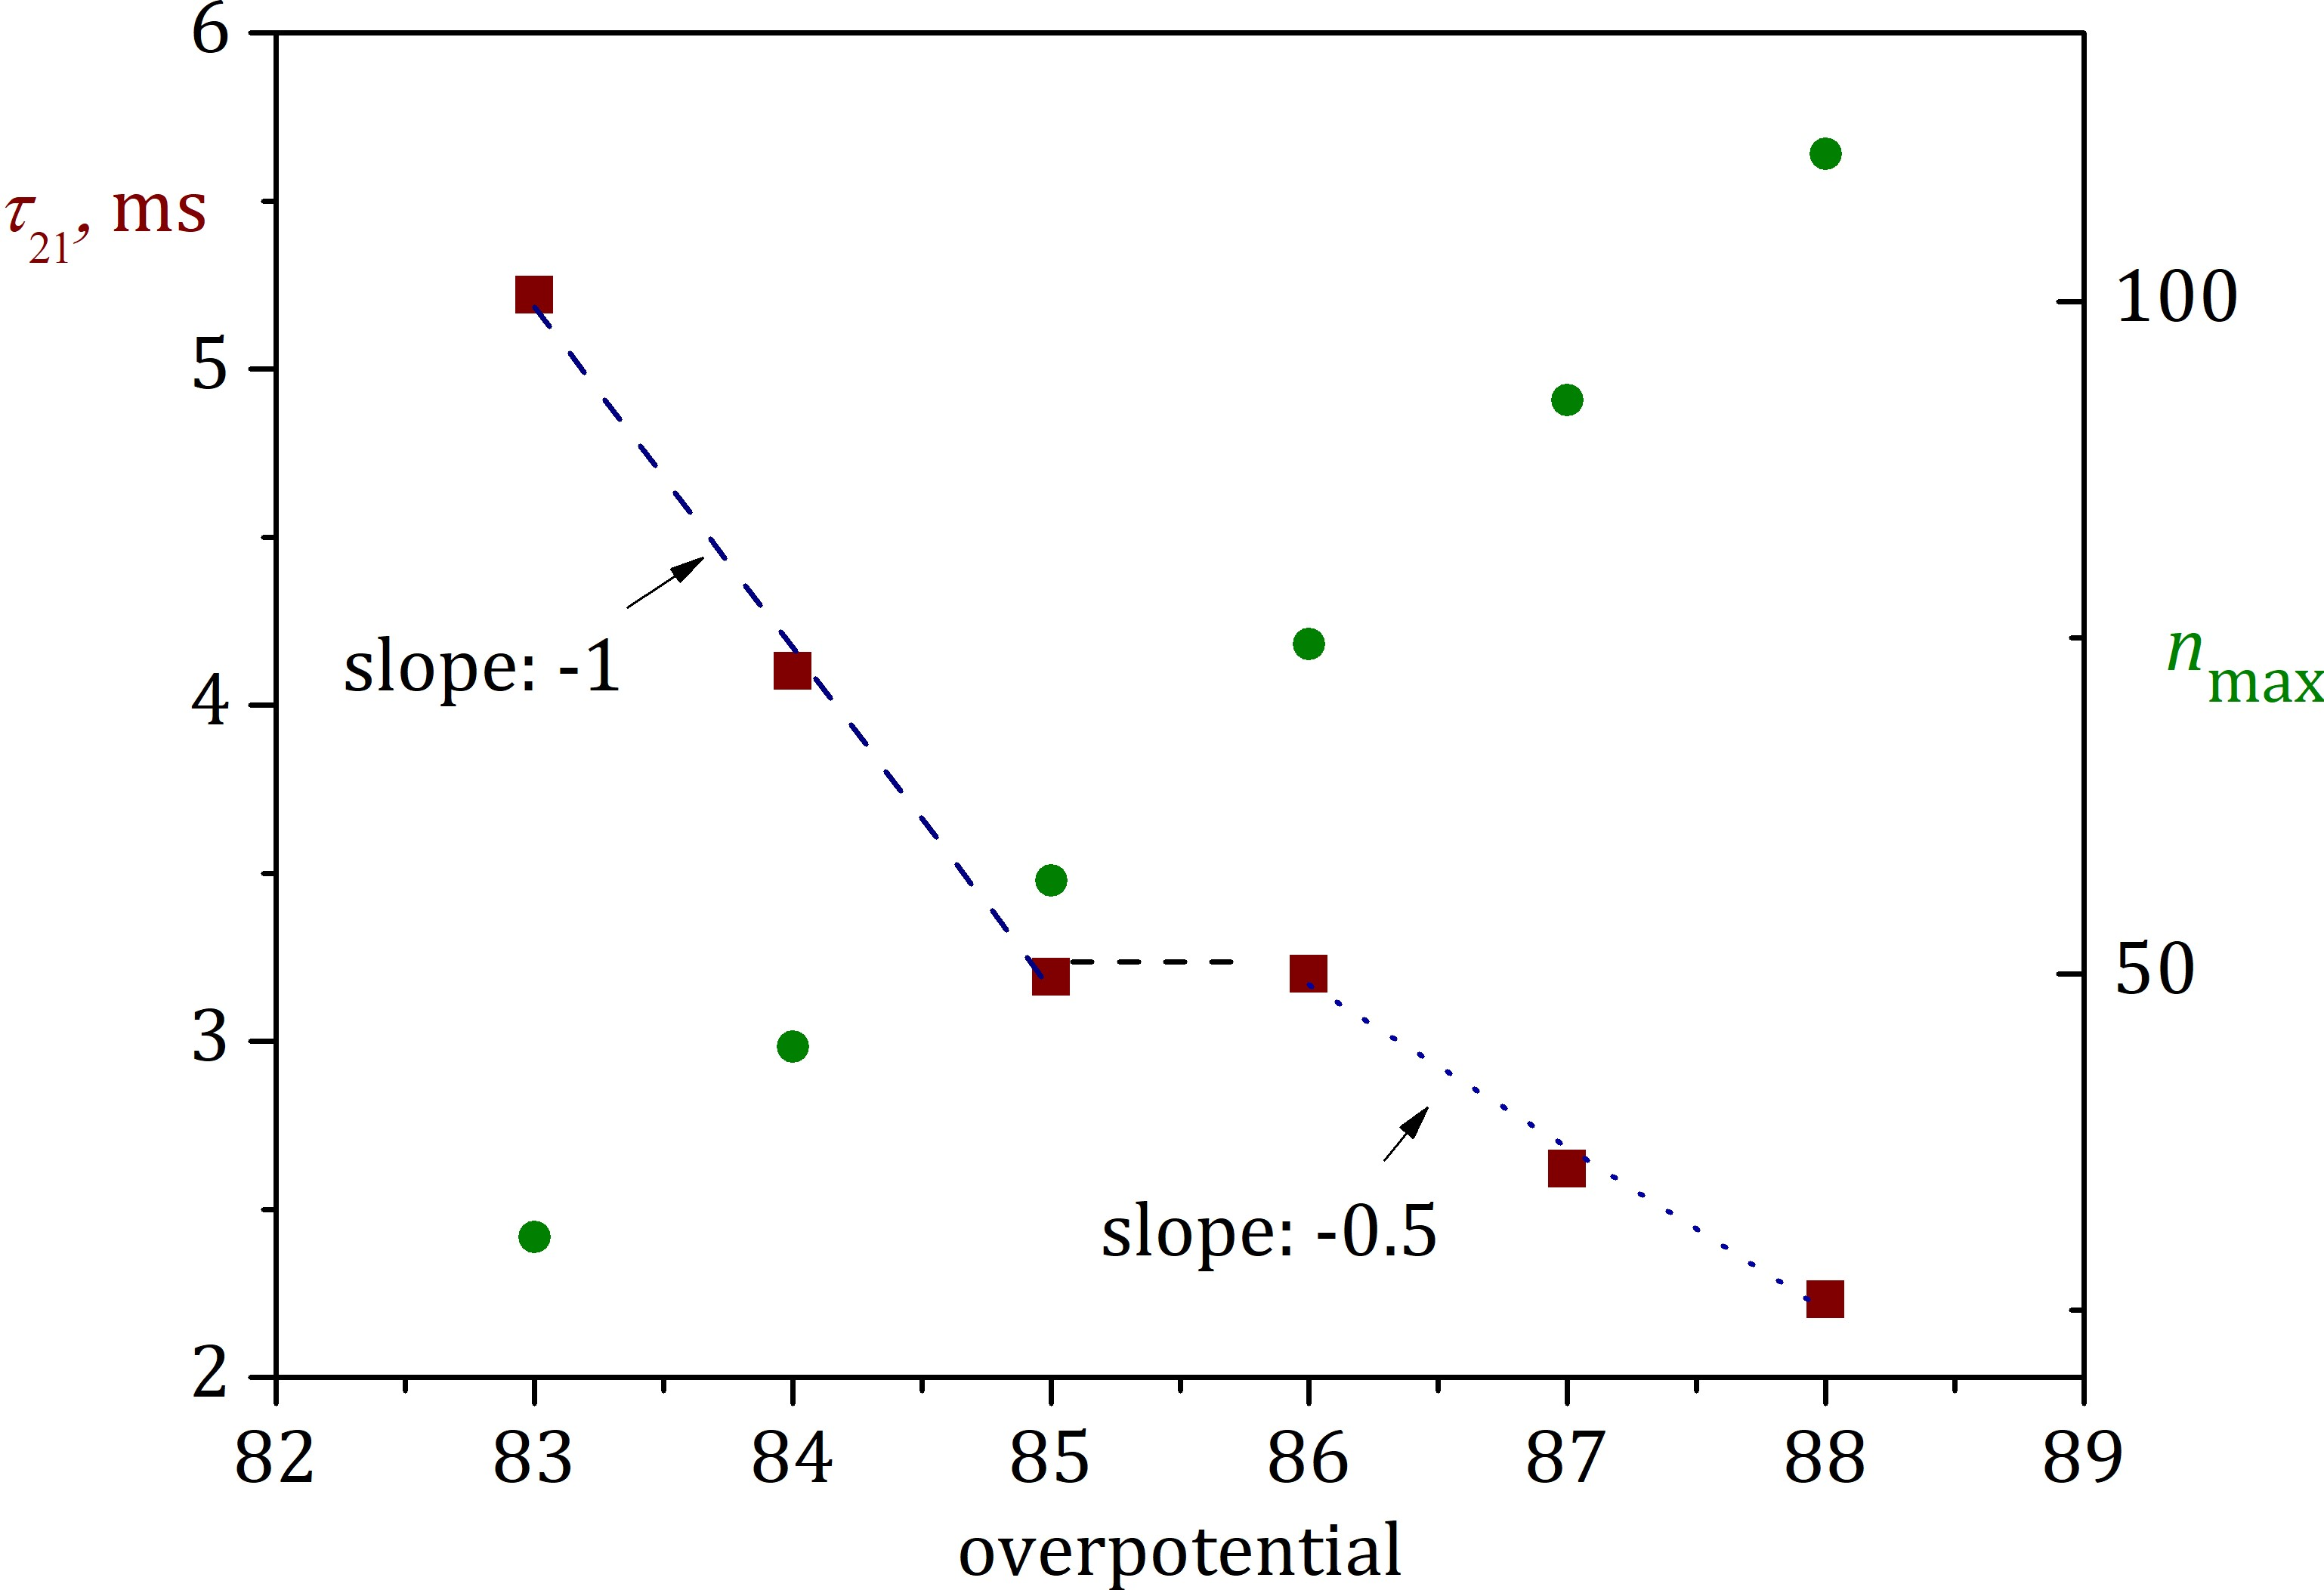
\includegraphics[width=0.48\textwidth]{ivan_markov_graphs/Fig5-alfa21_tau-overpotential.jpg}}
        \subfloat[Фиг. 6\label{subfig:alfa21_params_fig6}]{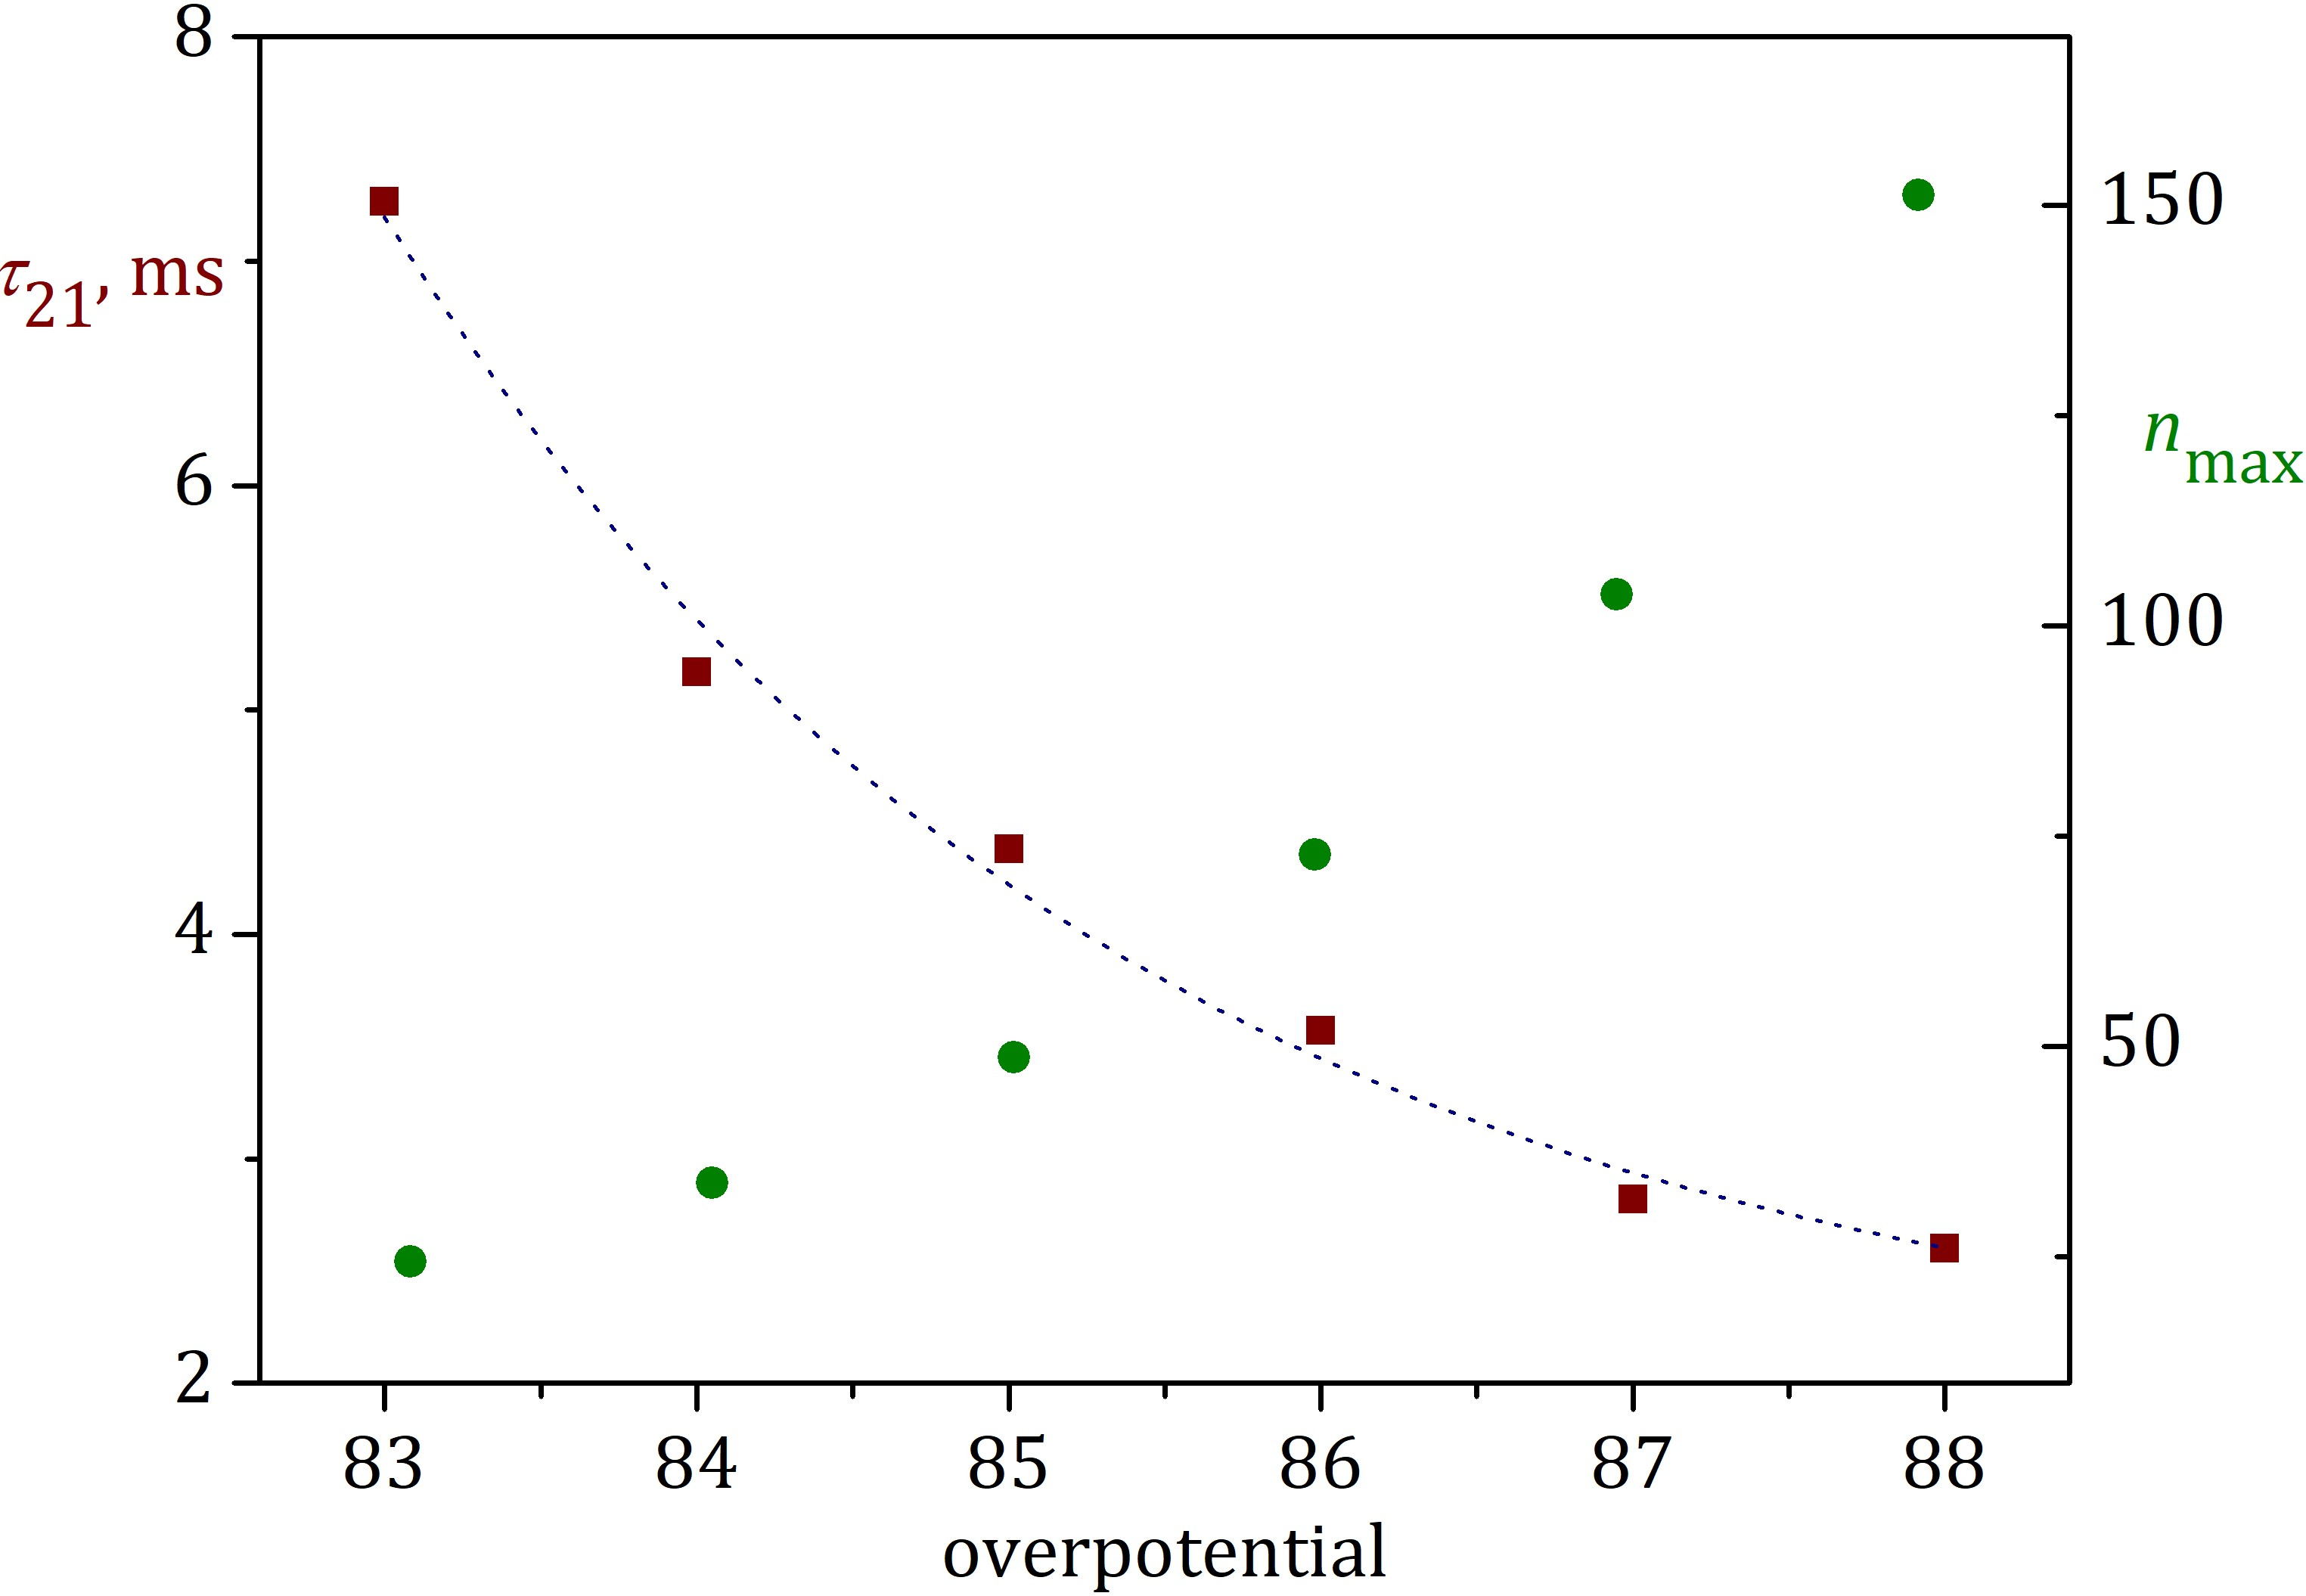
\includegraphics[width=0.48\textwidth]{ivan_markov_graphs/Fig6-alfa21_tau-overpotential.jpg}}  
    \caption[Зависимост на параметрите на модела от свръхпотенциала]{Зависимост на $N_{max}$ (\tikz\draw[darkgreen,fill=darkgreen] (0,0) circle (.5ex);) и $\tau_{21}$ (\tikz\draw[wine,fill=wine] (0,0) rectangle (1ex, 1ex);) от свръхпотенцила (пресищането) за $\alpha_{21}$}
    \label{fig:alfa21_ivan_markov_tau_nmax_overpot}
\end{figure}

\autoref{fig:alfa21_ivan_markov_tau_nmax_overpot} представлява връщането от безразмерна универсална крива - загуба на информация с цел потвърждаване на общия механизъм при различните експериментални условия. 

Изследването на зависимостта на скалите, с които е обезразмерен модела и как те зависят от свръхпотенциала (експерименталните условия) разкрива особености в поведението на системата.  На \autoref{subfig:alfa21_params_fig5} между $85~mV$ и $86~mV$ се наблюдава ясен сигнал за промяна на режима - наклонът на зависимостта $\tau_{21} (V)$ на практика намалява наполовина със скок. \autoref{subfig:alfa21_params_fig6} показва тъкмо обратното - гладко намаляване на характеристичното време $\tau_{21}$ с пресищането. В първия случай данните добре се описват от по части линейна зависимост, докато във втория - от квадратична.  Това поведение на $\tau_{21}$ във \autoref{fig:alfa21_ivan_markov_tau_nmax_overpot} може да бъде сравнено със спинодалния разпад в модела на Ван дер Ваалс за реалния газ (\textit{cusp catastrophy}).

При максималният брой зародиши подобна ,,катастрофа`` не се наблюдава в двата експеримента - и в двата случая имаме нарастване, което може да бъде описано с една гладка крива. На \autoref{subfig:alfa21_params_fig5} нарастването на максималният брой зародиши в системата $N_{max}$ е по-скоро линейно, докато \autoref{subfig:alfa21_params_fig6} е квадратично.

\subsubsection{Числени стойности на параметрите}

\begin{table}[htbp]
\centering
\caption{Данни за параметрите от фиг. 5 получени от моделите в йерархията. Скалата за Ричардс не е получена директно от фитването на данните. Параметрите $t_i$ и $t_k$ не са показани, тъй като не са използвани в дискусията на резултатите.}
\label{tabl:fig5_table_data}
\resizebox{\linewidth}{!}{%
\begin{tabular}{cccccccccccc} 
\toprule
\multirow{2}{*}{overvoltage, mV} & \multicolumn{3}{c}{$\alpha_{21}$}                                                           & \multicolumn{4}{c}{JMAKn}                                                                                                & \multicolumn{4}{c}{Richards}                                                                                           \\
                                 & \multicolumn{1}{l}{$N_{max}$} & \multicolumn{1}{l}{$\tau_{21}$} & \multicolumn{1}{l}{$R^2$} & \multicolumn{1}{l}{$N_{max}$} & \multicolumn{1}{l}{$\tau_{JMAKn}$} & \multicolumn{1}{l}{$n$} & \multicolumn{1}{l}{$R^2$} & \multicolumn{1}{l}{$N_{max}$} & \multicolumn{1}{l}{$\tau_{21}$} & \multicolumn{1}{l}{$q$} & \multicolumn{1}{l}{$R^2$}  \\ 
\hline
83                               & 30.43                         & 5.22                            & 0.9974                    & 29.9                          & 5.6                                & 1.89                    & 0.9977                    & 30.29                         & 5.20                            & 0.83                    & 0.9967                     \\
84                               & 44.61                         & 4.11                            & 0.9937                    & 45.78                         & 4.75                               & 1.39                    & 0.9986                    & 46.28                         & 3.93                            & 0.53                    & 0.9981                     \\
85                               & 56.94                         & 3.19                            & 0.9986                    & 56.86                         & 3.51                               & 1.67                    & 0.998                     & 57.36                         & 3.28                            & 0.64                    & 0.9984                     \\
86                               & 74.51                         & 3.20                            & 0.9976                    & 75.06                         & 3.61                               & 1.58                    & 0.9992                    & 75.60                         & 3.09                            & 0.79                    & 0.9988                     \\
87                               & 92.7                          & 2.62                            & 0.9988                    & 92.37                         & 2.89                               & 1.70                    & 0.9995                    & 93.17                         & 2.52                            & 0.96                    & 0.9989                     \\
88                               & 111.01                        & 2.23                            & 0.9974                    & 109.19                        & 2.40                               & 1.86                    & 0.999                     & 109.57                        & 2.09                            & 1.35                    & 0.9983                     \\
\bottomrule
\end{tabular}
}
\end{table}



\begin{table}[htbp]
\centering
\caption{Данни за параметрите от фиг. 6 получени от моделите в йерархията. Аналогично на Фиг.5 скалата за Ричардс е получена индиректно и параметрите $t_i$ и $t_k$ не са показани.}
\label{tabl:fig6_table_data}
\resizebox{\linewidth}{!}{%
\begin{tabular}{cccccccccccc} 
\toprule
\multirow{2}{*}{overvoltage, mV} & \multicolumn{3}{c}{$\alpha_{21}$} & \multicolumn{4}{c}{JMAKn}                  & \multicolumn{4}{c}{Richards}            \\
                                  & $N_{max}$ & $\tau_{21}$ & $R^2$   & $N_{max}$ & $\tau_{JMAKn}$ & $n$  & $R^2$  & $N_{max}$ & $\tau_{R}$ & $q$  & $R^2$   \\ 
\hline
83                                & 24.41     & 7.27        & 0.9966  & 23.92     & 7.79           & 1.91 & 0.9978 & 24.12     & 6.95       & 1.18 & 0.9963  \\
84                                & 33.84     & 5.17        & 0.9977  & 33.68     & 5.69           & 1.72 & 0.9978 & 33.93     & 4.98       & 0.93 & 0.9971  \\
85                                & 48.69     & 4.38        & 0.9969  & 48.97     & 4.92           & 1.55 & 0.9985 & 48.19     & 4.62       & 0.43 & 0.9987  \\
86                                & 72.78     & 3.57        & 0.9890  & 74.50     & 4.13           & 1.38 & 0.9967 & 73.07     & 3.36       & 0.51 & 0.9948  \\
87                                & 103.77    & 2.82        & 0.9923  & 106.51    & 3.30           & 1.38 & 0.9993 & 103.81    & 2.68       & 0.54 & 0.9990  \\
88                                & 151.22    & 2.60        & 0.9891  & 156.27    & 3.03           & 1.35 & 0.9971 & 151.30    & 2.43       & 0.52 & 0.9958  \\
\bottomrule
\end{tabular}
}
\end{table}
\autoref{tabl:fig5_table_data} и \autoref{tabl:fig6_table_data} показват, че на практика за всеки от моделите и наборите данни $R^2 \approx 0.99$, т.е. по този критерий (остатъчна дисперсия) те трудно могат да бъдат разделени. Максималният брой зародиши $N_{max}$ и времевите скали $\tau$ също са близки за всяка от колоните на таблиците (трудно можем да различим експериментално $N_{max} = 72, 74.5, 73$ например). Определящ тогава ще е изцяло броят параметри и физичният смисъл, който стои зад тях. 

При JMAKn не можем да дадем физическо обяснение за получените оптимални стойности за $n$, a фиксирането на $n = 2$ води до значително влошаване на $R^2$. Аналогично, при моделът на Ричардс стойностите за $q$ не преполагат нито класически логистичен растеж, нито по модела на Гомперц. Фиксирането на този параметър също значително влошава $R^2$, като и физическото обяснение на параметрите е още по-трудно от това за JMAKn.

Изборът на конкретно кривата $\alpha_{21}$ \textit{a priori} предполага дифузионно контролиран квази-двумерен растеж, каквито и са заложените в експеримента условия. Параметрите $N_{max}$ и $\tau_{21}$ са напълно ясни в своя смисъл. Нещо повече - те представляват скалите за брой зародиши $N$ и време $t$, което позволява да получим универсалното поведение показано на \autoref{fig:alfa21_ivan_markov_master_curve}. 

За JMAKn и Ричардс параметрите не очертават ясна зависимост от свръхпотенциала. Експонентите $n$ и $q$ съответно и в двата случая намаляват и се насищат при високи потенциали. Скалите в този случай можем да сравняваме и не очертават ясна зависимост. При, $\alpha_{21}$ както беше показано в предния параграф, се наблюдава интересна зависимост на времевата скала от експерименталните условия, което може да бъде оснонова на бъдещи изследвания.
\section{Моделиране на тангенциалния растеж на повърхността}
До момента показаните модели дават връзки за напредването на кристалната стена в безпорядъчната фаза, т.е. нормалния растеж на стената и съответната нормална скорост. В \autoref{sub:microscopic_growth} беше показано, че микроскопският механизъм на нарастване на кристалите е обусловен от свързването към кинк-позиция и изграждане на стената слой по слой. По тази причина фокусът ще бъде преместен към моделиране микроскопските процеси, които протичат при растеж на кристалите и детайлите свързани с това. Конкретният физичен процес, който ще бъде обект на разглеждане е т.нар. групиране на повърхностните ,,стъпала`` при растеж - \textit{step bunching}.
\subsection{Вицинални повърхности}
Атомите, йоните и молекулите от гледна точка на кристалния растеж и нашите разглеждания са неделими, дискретни структури. За приготвянето на повърхности за целите на насочен кристален растеж, често голям монокристал се срязва на тънки плоскости или дискове (\autoref{fig:sillicon_wafers}). Например за целите на производството на фотоволтаични клетки се изрязват тънки пластинки от свръхчист силициев монокристал, при които чрез т.нар. процес на \textit{епитаксия} (насочен послоен растеж) се изграждат допълнителни повърхностни слоеве, придаващи нужните свойства на кристала.
\begin{figure}[htbp]
	\centering
	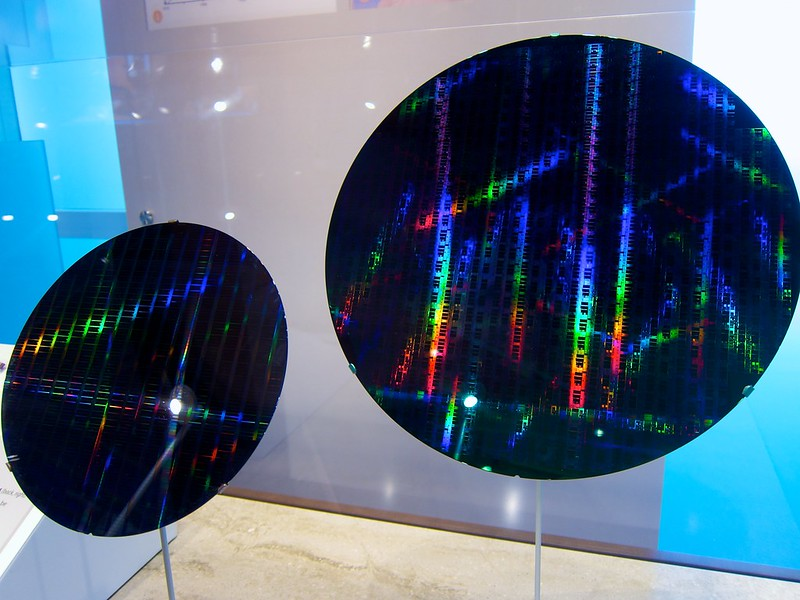
\includegraphics[width=0.5\textwidth]{silicon-wafers.jpg}
	\caption{Пластинки изрязани от силициев монокристал използвани за производството на компютърни чипове. \cite{debold_waffers_2011}}
	\label{fig:sillicon_wafers}
\end{figure}
Поради неделимата структура на градивните единици обаче следва, че няма как технологичният инструмент да среже ,,през атома``, т.е. получената повърхност при срязването на монокристала няма как да бъде гладка на атомно ниво, а се формират т.нар. \textit{стъпала}, a самата повърхност наричаме \textit{вицинална}.
\begin{figure}[htbp]
	\centering
	
\includegraphics[width=\textwidth]{miscut.png}
	\caption{Схематично представяне на срязването на монокристал под ъгъл $\theta$}
	\label{fig:miscut_crystal}
\end{figure}

Ще различаваме между две основни структури, които са допълнителни на вициналната повърхност - тераси (непрекъснати части от повърхността с еднаква височина) и стъпала - преходите между две тераси. Ъгълът, под който е срязан монокристала дава началната ширина на терасите (разстояние между стъпалата) - $l_0$. Да обърнем внимание, че при постоянен ъгъл на срязване началното $l_0$ e еднакво за всички тераси. Такава вицинална повърхност с равномерно отдалечени стъпала ще бъде и началното условие за всички модели, които ще разгледаме.
\begin{figure}[htbp]
	\centering
	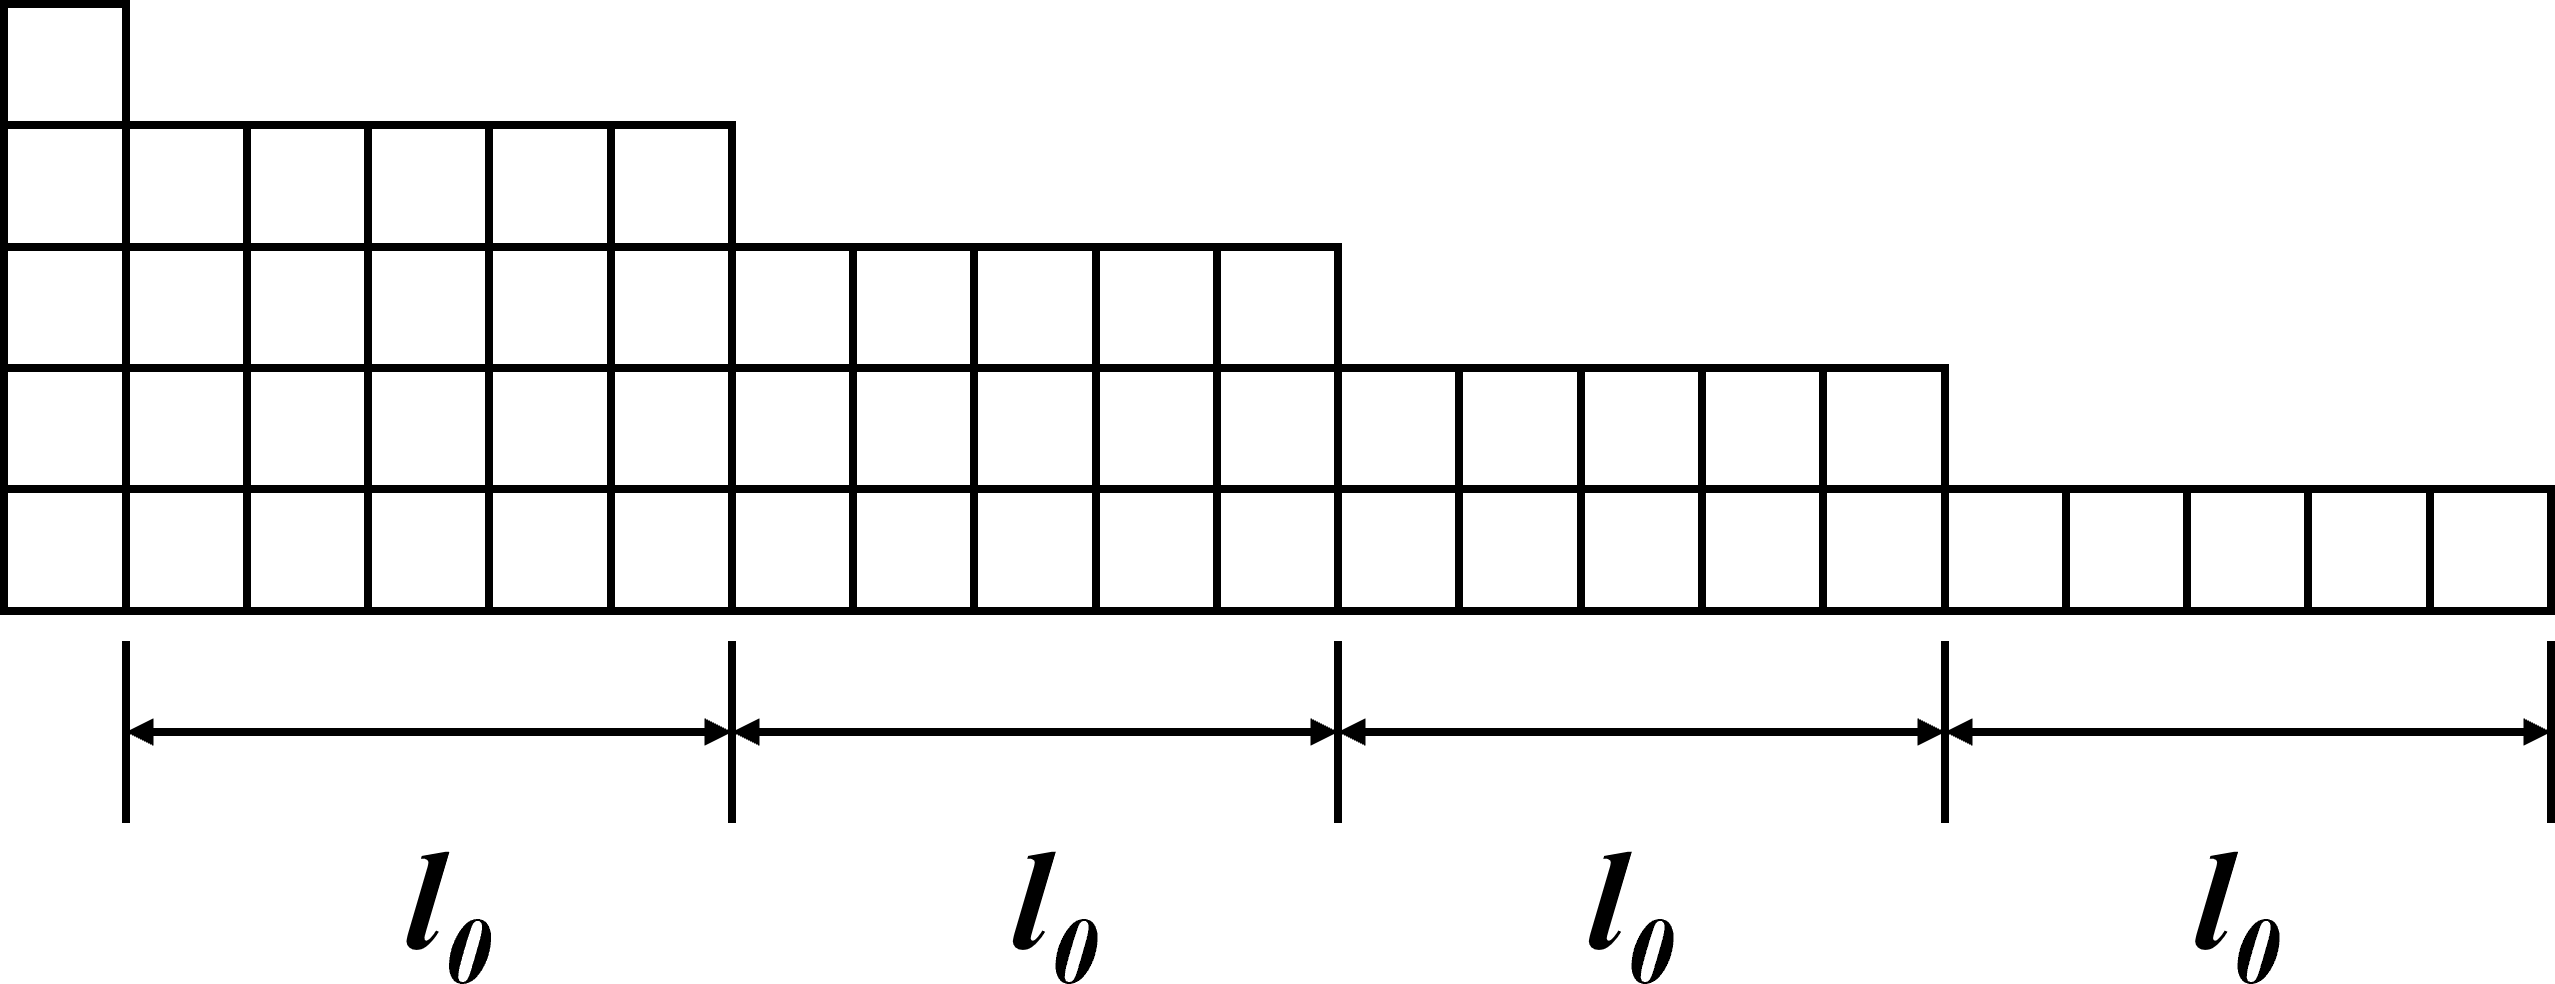
\includegraphics[width=\textwidth]{vicinal.png}
	\caption{Схематично представяне на вициналната повърхност. С $l_0  \propto \cot{\left( \theta \right)} $ e отбелязано началното вицинално разстояние между стъпалата (ширина на терасите).}
	\label{fig:initial_vicinal}
\end{figure}

\autoref{fig:miscut_crystal} и \autoref{fig:initial_vicinal} представят цялостния процес на формиране на една вицинална повърхност и ще служат като основа na следващите модели. Да обърнем внимание, че на една такава двумерна вицинална повърхност всяко от стъпалата всъщност представлява кинк-позиция. В 3D (вж. \autoref{fig:atoms_on_surface}) не е задължително всяка позиция на стъпало да бъде кинк позиция.
\subsection{Групиране на стъпалата (step bunching)}
През 1989~г. в статия от \textit{Latyshev et. al} \cite{Latyshev1989} е описано за пръв път т.нар. групиране на стъпала при растеж и/или сублимация (\textit{step bunching)} на кристалната повърхност на Si(111) в електрично поле. Започвайки от начална вицинална повърхност като показаната на \autoref{fig:initial_vicinal}, по време на процеса на растеж се наблюдава ефективно ,,придвижване`` на стъпалата по повърхността на растящия кристал, така че разстоянието между тях $l_{bunch}$ намалява спрямо началното вицинално разстояние $l_{bunch} < l_0$, като така се формират групи от стъпала на повърхността. Тези групи са разделени една от друга от тераси, чиято ширина е по-голяма от началната $l_{terrace}  > l_0$.
\begin{figure}[htbp]
	\centering
	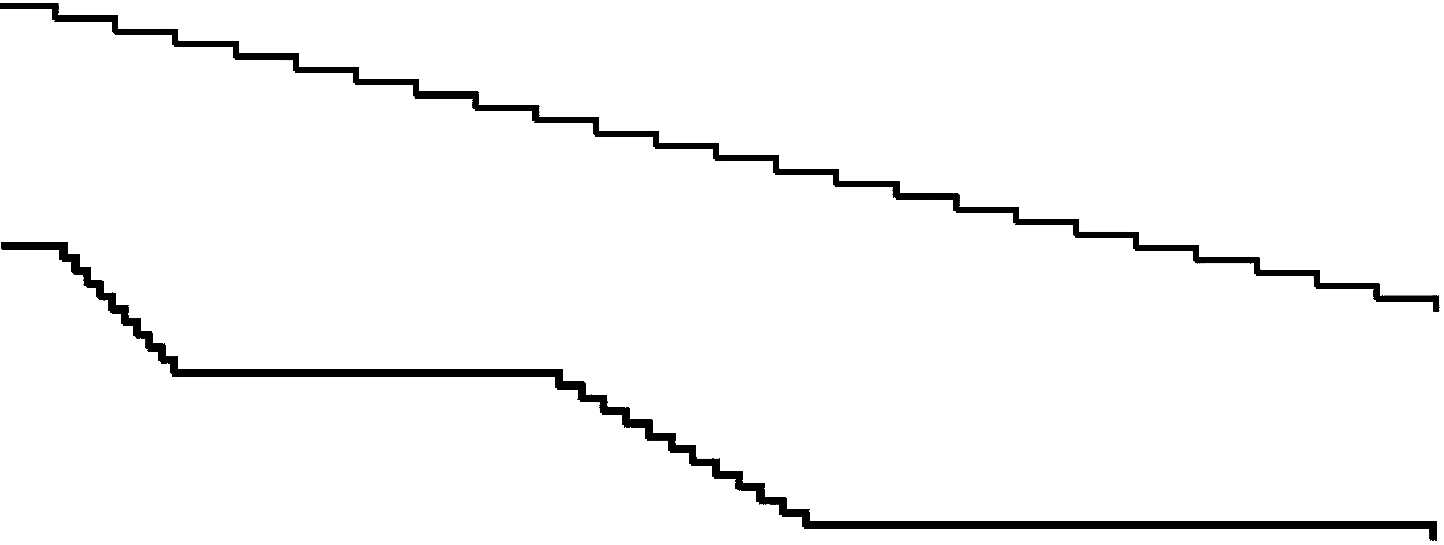
\includegraphics[width=\textwidth]{step_bunching_scheme.png}
	\caption{Схематично представяне на групиране на стъпалата върху кристалната повърхност. От начална вицинална повърхност с равни начални разстояния между стъпалата са формирани две групи в които $l_{bunch} < l_0$.}
	\label{fig:step_bunching}
\end{figure}
За да наблюдаваме такъв процес на реорганизация на повърхността, трябва в системата да съществува нестабилност, обуславяща движението на стъпалата едно спрямо друго. В литературата \cite{StoyanStoyanov1991}\cite{TonchevArxiv2012} са идентифицирани два основни източника на нестабилност при кристализация и изпарение - \textit{Ерхлих-Швьобелов ефект} (локален ефект) \cite{Ehrlich1966} \cite{Schwoebel1966} и електромиграция (обемен ефект) \cite{Latyshev1989}. Поради това в следващите параграфи ще разгледаме физиката зад тези два ефекта.
\subsubsection{Ерлих-Швьобелов (ЕШ) ефект}
Този ефект представлява представлява разлика в енергиите на свързването или отделянето на градивна единица към предната и задната тераса. Ефектът е локален и зависи от размера на терасите
отгоре и отдолу на стъпалото \cite{Krug2005}. Когато свързването е преференциално към предната тераса, ефектът се нарича \textit{нормален} (прав) Ерлих-Швьобелов ефект,  докато ако свърването е преференциално към задната - \textit{обратен} Ерлих-Швьобелов ефект. При растеж на метални кристални решетки е до голяма степен повсеместен нормалният ЕШ ефект, докато при полупроводници като Si(111) при високи температури се наблюдава обратния ЕШ, а при ниски - нормалният.
Този ефект води до нестабилност в системата - двете тераси, формиращи едно стъпало нарастват с различна скорост - това създава ефективно движение ,,напред`` на стъпалото и намаляване на разстоянието между стъпалата $l_{bunch} < l_0$.
\begin{figure}[htbp]
	\centering
	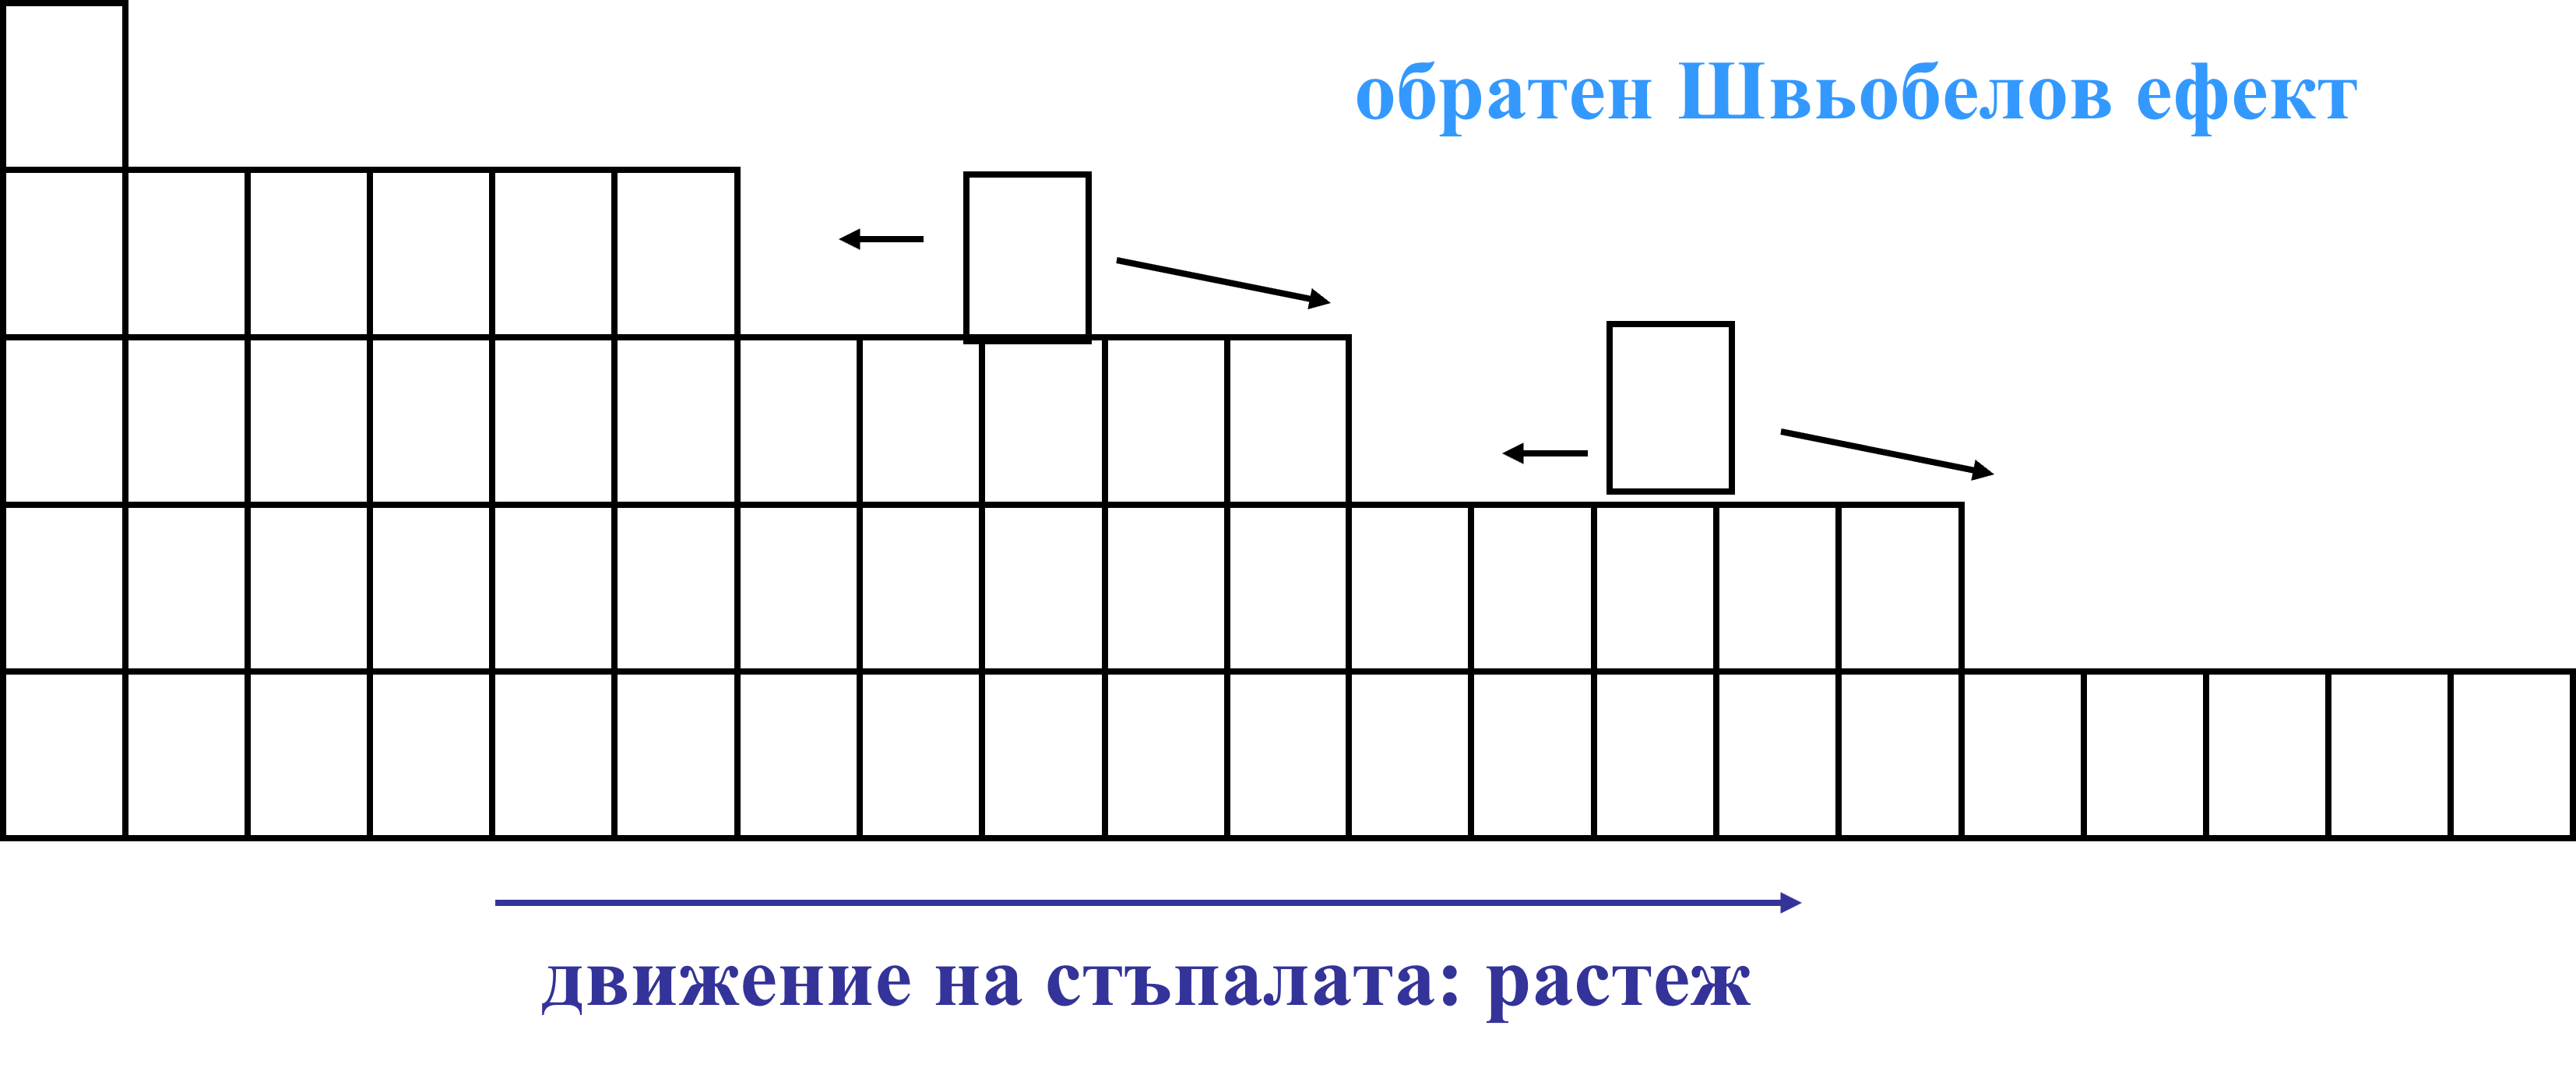
\includegraphics[width=\textwidth]{reverse_schwobel_effect_bunching.png}
	\caption{Обратен ЕШ ефект водещ до групиране на стъпалата при кристализация. Тук условно посоката на нарастване (кристализация) е взета да е надолу (надясно).}
	\label{fig:inverse_es_effect}
\end{figure}

На \autoref{fig:inverse_es_effect} e показано как обратният ЕШ при кристализация е ,,източник на нестабилност`` - задната тераса допринася повече към движението на стъпалото от предната (условно отбелязано с дължината на стрелките сочещи към съответната тераса). Съответно пертурбирайки задната тераса за $i$-тото стъпало напред (нараства с една градивна единица), това води до увеличаване на ефективната скорост на $i$-тото стъпало поради обратния ЕШ ефект. Пертурбирайки предната за $i$-тото стъпало тераса напред, тя се явява задна за $i+1$-вото стъпало и неговата скорост се увеличава. Обобщено, независимо към коя тераса се свърже градивната единица, обратния ЕШ е източник на нестабилност при кристализация.
\begin{figure}[htbp]
	\centering
	\includegraphics[width=\textwidth]{normal_schowbel_effect.png}
	\caption{Нормален ЕШ ефект водещ до групиране на стъпалата при изпарение. Тук условно посоката на изпарение (сублимация) е взета наляво (нагоре).}
	\label{fig:normal_es_effect}
\end{figure}

\autoref{fig:normal_es_effect} показва обратния на кристализацията случай - изпарението, тук нормалният ЕШ ефект действа в обратна посока (нагоре). Чрез аналогични разсъждения за пертурбиране на стъпалата може да се покаже, че нормалният ЕШ е източник на нестабилност при изпарение. Тук различното е, че градивните единици ще се откъсват от съответната им тераса.

ЕШ е \textbf{локален ефект}, който води до нестабилност в системата. За него най-важното е, че той е насочен нагоре или надолу по терасите в зависимост от това дали разглеждаме кристализация или сублимация.  В случая, когато имаме нормален ЕШ при растеж се наблюдава друг интересен режим на нестабилност на вициналната повърхност - меандриране. Меандрирането също е особен ефект и изисква собствено изучаване, което не е цел на настоящия труд. \cite{Krug2005} Следващият ефект, който ще разгледаме - \textit{електромиграцията}, насочена в една и съща посока тя е източник на нестабилност и за растеж, и за изпарение.

\subsubsection{Електромиграция}
Електромиграцията е процес на пренос на заредени частици под действието на електрично поле. В контекста на кристализация и по-конкретно - групиране на стъпала, електричното поле създава насочено движение (адвекция) на градивни частици по посока на нарастване на потенциала.
За разлика от нормалния и обратния ЕШ ефект, елеткромиграцията е \textit{обемен} ефект - това означава, че силата, която действа на атомите се характеризира изцяло с векторното поле на електричния потенциал $\overline{f}$ и не зависи от размера на съседните на $i$-тото стъпало тераси. Допълнително - електромиграцията е източник на нестабилност и води до съответно групиране на стъпалата при една и съща посока на силата (напр. надолу) за случаите на кристализация и сублимация.

\autoref{fig:electromigration_crystalization} и \autoref{fig:electromigration_sublimation} илюстрират поведението на системата при нестабилност вследствие електромиграция. Електричното поле води до преференциално свързване към задната на $i$-тото стъпало тераса при групиране и отделяне от предната за $i$-тата тераса при сублимация, така резултатът и в двата случая е групиране на стъпалата при еднаква посока на силата.
\begin{figure}[htbp]
	\centering
	\includegraphics[width=\textwidth]{electromigration_growth.png}
	\caption{Електромиграция насочена условно надолу при кристализация, водеща до преференциално свързване към задната тераса и групиране.}
	\label{fig:electromigration_crystalization}
\end{figure}
\begin{figure}[htbp]
	\centering
	\includegraphics[width=\textwidth]{electromigration_sublimation.png}
	\caption{Електромиграция насочена условно надолу при сублимация, водеща до преференциално отделяне от предната тераса и групиране.}
	\label{fig:electromigration_sublimation}
\end{figure}

\subsection{Динамика на адатомите}
Динамиката на стъпалата може да се разглежда като задача с подвижна граница (moving boundary problem), като самото стъпало е идеализирана математическа граница между две съседни тераси (скок във функцията описваща локалната височина на повърхността), която еволюира чрез обмен \textit{през} непрекъснатото поле на адатомите в околността на повърхността $N(\overline{x}, t)$. $N$ - брой адатоми в полето, $\overline{x}$ - координата в пространството над повърхността, $t$ - време. \cite{Krug2005} Ще разгледаме модел на групиране под електромиграция, тъй като обемният характер на силата прави този случай по-прост.
Нека отбележим с $D = const$ - дифузионния коефициент на адатомите, $k_B$ - болцманова константа, $Т$ - абсолютна температура, $\overline{f}$ - сила на електромиграция, $G$ - поток на отлагане на адатомите, $\tau$ - характеристично време на отлагане. Комбинирани тези ефекти дават за еволюцията на адатомното поле:
\begin{equation}
	\label{eq:advection_diffusion_adatom_dynamics}
	\frac{\partial N}{\partial t} = D \nabla^2 N - \frac{D}{k_B T} \overline{f} \cdot \nabla N + G - \frac{N}{\tau} = - \nabla \cdot J + G - \frac{N}{\tau}
\end{equation}
\autoref{eq:advection_diffusion_adatom_dynamics} e уравнение от вида адвекция-дифузия. Обобщеният поток на адатомите тогава е:
\begin{equation*}
	J = -D \nabla N + \frac{D}{k_{B} T} \overline{f} N
\end{equation*}
\begin{equation*}
	\nabla \cdot \overline{f} = 0
\end{equation*}
Коефициентът $D/(k_{B} T)$ се нарича подвижност на адатомите. 

Докато самото ЧДУ е стандартно от математическа гледна точка, особени са граничните условия върху стъпалата. Те са условия на Робин за локалния поток върху границите на терасата. Нека $j_+$ е локалният поток върху отляво на терасата (прииждащ по посоката на кристализация), а $j_-$ е този отдясно (напускащ). Обикновено те са рескалирани спрямо локалния равновесен брой адатоми:
\begin{align*}
	j_+ &= k_+ (N_+ - N_{eq}) + p (N_+ - N_{eq}) \\
	j_- &= k_- (N_- - N_{eq}) + p (N_- - N_{eq}) 
\end{align*}
Където $k_+$ и $k_-$ са склонностите за свързване към двете стъпала, а $p$ e т.нар. \textit{прозрачност} на стъпалото. Тогава, на база закона за материалния баланс в система, получаваме следните г.у. за потоците $j_+$ и $j_-$.

\begin{align*}
	j_+  &= D \overline{n} \left[ \nabla N|_+ - \frac{1}{k_B T} \overline{f} N \right] \\
	j_-  &= - D \overline{n} \left[ \nabla N|_- - \frac{1}{k_B T} \overline{f} N \right] 
\end{align*}
Където $\overline{n}$ е единичната нормала към стъпалото, която сочи към долната тераса, а  $N|_\pm$ са броя адатоми от двете страни на стъпалото \cite{Krug2005}.
\textit{Стоянов} \cite{StoyanStoyanov1991} решава \autoref{eq:advection_diffusion_adatom_dynamics} в едномерния (1D+t) случай и показва, че когато електромиграцията е насочена надолу по стъпалата (по посока на кристализацията), действително се наблюдава групиране в този модел. 

Подвижните гранични условия в тази задача я правят значително сложна дори за числено изследване в по-голям брой измерения - 2D + t, 3D + t. 

Затова за 1D+t случая може да се направи значително опростяване като повърхността се сведе до едномерна такава, като в началото на всяка позиция $X_i, i = \overline{1,N}$ имаме стъпало. Така ще получим един окрупнен модел под формата на ОДУ, в който стъпалата от \autoref{fig:step_bunching} са заместени с точки (техните позиции) върху числова ос.

\subsection{ОДУ модел за скоростта на стъпалата}
\begin{figure}[htbp]
	\centering
	\includegraphics[width=\textwidth]{step_growth_direction.png}
	\caption{Схематично представяне на модела. За положителна посока по $x$-приемаме посоката ,,надолу`` по стъпалата. С $x_{i}, i = \overline{1, N}$ означаваме позициите на съответните стъпала.}
	\label{fig:step_growth_ode_model_scheme}
\end{figure}
Нека спрямо \autoref{fig:step_growth_ode_model_scheme} да приемем, че на всяка позиция $x_{i}$ имаме стъпало. Разликата във височината между всяко стъпало да е една градивна единица и в началото, те да са на равно разстояние едно от друго $l_0$ - началното вицинално разстояние. Допълнително, нека:
\begin{equation*}
    \Delta x_i \coloneqq x_i - x_{i - 1}
\end{equation*}
Това e ширината на $i$-тата тераса - тази за която $i$-то стъпало е долното такова.
Тогава за скоростта на $i$-тото стъпало можем да запишем в най-общ вид ОДУ, чието н.у. е началната вицинала с периодични г.у. (първото стъпало \textbf{е до} N-тото) \cite{Krasteva2016}:
\begin{equation}
    \frac{d x_i}{d t} = k a_i + u r_i
    \label{eq:general_step_velocity_ode}
\end{equation}
Където с $a_i$ сме обозначили функция на $\Delta x_{i-n}, \Delta x_{i-n + 1}, ..., \Delta x_{i}, ... \Delta x_{i + n} $ отчитаща обобщено силите на привличане, а с $r_{i}$ - функция на  $\Delta x_{i-n}, \Delta x_{i-n + 1}, ..., \Delta x_{i}, ... \Delta x_{i + n}$ (големината на $n$-те задни и $n$-те предни тераси) - отчитаща силите на отблъскване. В общия случая се разглеждат до първи и втори съседи $n = 0,1$. Параметрите $k$ и $u$ са константите на пропорционалност между двете сили (безразмерни). Конкретни изрази за $a_i, r_i$ ще бъдат дадени по-нататък. 

\subsubsection{Автомоделни решения}
Искаме да намерим автомоделни решения \cite{Barenblatt1996} \cite{Krasteva2016}:
\begin{equation}
    t^\delta l = s_{l t} 
    \label{eq:dimensional_scaling}
\end{equation}

Където $l(t)$ e характеристично за групите разстояние (напр. $l_{min}$ - минимално разстояние в дадена група),  $s_{l t} = f(k, u, l_0)$ е автомоделната функция. Тя следва да е функция на параметрите на модела $k, u$ и началното разстояние $l_0 = l_{min} (0)$. Тук $\delta$ е времевата експонента на динамичния скейлинг и e безразмерна величина \cite{Vicsek1984}. Такива автомоделни решения описват самоподобието на групите, които се формират:
\begin{equation*}
    l(t_1) t_1^\delta = l(t_2) t_2^\delta
\end{equation*}
Записано във вида \autoref{eq:dimensional_scaling} показва, че за размерността на автомоделната функция имаме:
\begin{equation*}
    \left[s_{l t} \right] = T^\delta L
\end{equation*}
Където T, L са съответно размерностите за време и дължина. За да отговаря на анзаца на \textit{Family-Visceck}, искаме да обезразмерим това уравнение и да получим скейлинговата функция в ,,чист вид``. За целта ще започнем с обезразмеряването на \autoref{eq:general_step_velocity_ode}.
Ще дефинираме безразмерното разстояние и време съответно:
\begin{align*}
    X_{i} & \coloneqq \frac{x_i}{\xi_0} \\
    T & \coloneqq \frac{t}{\tau_0}
\end{align*}
Тук обезразмеряванията и скалите $\xi_0, \tau_0$ са въведени естествено, без ограничение на общността на уравнението.
Ще направим \textit{допускането} че $[a_i] = L ^ \nu $ и $[r_i] = L ^ \mu$, т.е. в размерността им единствено участва дължината. Това означава, че тези сили на привличане и отблъскване зависят от времето единствено чрез размера на терасите в дадения момент, което не е силно ограничение в общността и е физически обосновано допускане (кохерентност на групите). Тогава дефинираме безразмерните сили на взаимодействие:
\begin{align*}
    A_{i} & \coloneqq \frac{a_i}{\xi_{0}^ \nu} \\
    R_{i} & \coloneqq \frac{r_i}{\xi_{0}^ \mu}
\end{align*}
Заместваме и получаваме:
\begin{equation*}
    \frac{\xi_0}{\tau_0} \frac{d X_i}{d T} = \xi_0^\nu k A_i + \xi_0^\mu u R_i
\end{equation*}
\begin{equation*}
    \frac{d X }{d T} = \tau_0 \xi_0^{\nu-1} k A_i + \tau_0 \xi_0^{\mu-1} u R_i
\end{equation*}
Тъй като досега не сме допуснали нищо за $\tau_0, \xi_0$ ще ги изберем така, че в основното ОДУ да няма експлицитно параметри. Така имаме системата от уравнения за скалите:
\begin{equation}
    \begin{cases}
        \tau_0 \xi_0^{\nu-1} k = 1 \\
         \tau_0 \xi_0^{\mu-1} u = 1
    \end{cases} 
\end{equation}
Решаваме системата за скалите и получаваме:
\begin{align*}
    \xi_0 &= \left( \frac{u}{k} \right)^ {\frac{1}{\nu - \mu}} \\
    \tau_0 &= k^{-1} \left( \frac{u}{k} \right) ^ {\frac{1-\nu}{\mu - \nu}}
\end{align*}
И обезразмерено диференциалното уравнение:
\begin{result}{Oбезразмерен общ ОДУ модел на групиране}{ode_general}
    \begin{equation}
        \label{eq:non_dimenisonal_ode}
        \frac{d X_i}{d T} = A_i + R_i
    \end{equation}
\end{result}
С обезразмерено начално разстояние: $L_0 \coloneqq \frac{l_0}{\xi_0}$.
Можем сега да получим и безразмерната форма на \autoref{eq:dimensional_scaling}.
\begin{align*}
    l t^\delta &= s_{l t}(l_0, k, u) \\
    \frac{l}{\xi_0} \left(\frac{t}{\tau_0}\right)^{\delta} &= L T ^\delta = S_{L T} (L_0)
\end{align*}
Където $L \coloneqq \frac{l}{\xi_0}$, $T \coloneqq \frac{t}{\tau_0}$. Заместваме скалите, извършваме алгебричните преобразования и получаваме \cite{Krasteva2016}:
\begin{equation*}
    l t ^ \delta =  \left( \frac{u}{k} \right)^ {\frac{1}{\nu - \mu}} k^{-\delta} \left( \frac{u}{k} \right) ^ {\delta \frac{1-\nu}{\mu - \nu}} S_{L T} (L_0)
\end{equation*}
Където $S_{L T}$ е безразмерната автомоделна функция, която зависи \textbf{само} от обезразмереното начално разстояние $L_0$.

С проведената процедура по обезразмеряване на задачата постигнахме следното:
\begin{itemize}
    \item Намерихме ,,естествените`` скали на задачата.
    \item В основното ОДУ нямаме параметри.
    \item Намалихме параметрично пространство от $(k, u, l_0)$ на едномерното - $(L_0)$.
    \item Получихме автомоделна функция $S_{L T}$, която зависи \textit{само} от началното разстояние $L_0$.
\end{itemize}

Освен аналитичните резултати как влияят параметрите на модела върху решения от вида на \autoref{eq:dimensional_scaling}, това обезразмеряване значително намалява необходимите изчисления за числено изследване на модела при различен конкретен вид на привличането и отблъскването на стъпалата. Ако в размерната версия например правим по 10 ,,експериментални резултата`` за всеки параметър, то общо ще са ни необходими 1000 числени експеримента, при безразмерния модел - само 10, т.е. сложността на задачата е намалена от $O(n^3)$ до $O(n)$.

\subsubsection{Изрази за силите на привличане и отблъскване}
Във времето са разработени разнообразни ОДУ модели в литературата по групиране, които отговарят на общия вид зададен от \autoref{eq:non_dimenisonal_ode}. Те обикновено са публикувани в размерена форма и параметрите $k, u$ в тях могат да имат сложен ви. Най-важното за всеки от тях е, че $k, u$ не зависят от размера на терасите. Те например могат да носят зависимостта от температурата, да отчитат материалните характеристики на повърхността и т.н.

Ще разгледаме безразмерните форми на моделите на \textit{Liu \& Weeks} (1998) \cite{Liu1998} (\textbf{LW2}), \textit{Tersoff} (1995) \cite{Tersoff1995} (\textbf{TE}) и \textit{ad-hoc} минимален модел на \textit{Тончев \& Кръстева} (2016) \cite{Krasteva2016} (\textbf{MM2}) - минимална част от модела на \textit{Liu \& Weeks} (1998), така че да може да бъде получено групиране. Изрази за трите модела са дадени в \autoref{tabl:rhs_bunching_ode}.

\begin{table}[hbpt]
\resizebox{\textwidth}{!}{
\begin{tabular}{@{}ccc@{}}
\toprule
 &
  $A_i$ &
  $R_i$ \\ \midrule
\textbf{MM2} &
  $-F_i^{- (p + 1)} \coloneqq -\left(  \Delta X_i^{-(p+1)} - \Delta X_{i+1} ^{-(p+1)} \right)$ &
  $F_i^{- (n + 1)} \coloneqq  \Delta X_i^{-(n+1)} - \Delta X_{i+1} ^{-(n+1)}$ \\
\textbf{LW2} &
  $F_{i+1}^{-(p+1)} - 2 F_{i}^{-(p+1)} + F_{i-1}^{-(p+1)}$ &
  $- \left( F_{i+1}^{-(n+1)} - 2F_{i}^{-(n+1)} + F_{i-1}^{-(n+1)}  \right)$ \\
\textbf{TE} &
  - $\left[ \Delta X_{i+1}^{-1} \left( F_{i+2}^{-(p+1)} - F_{i+1}^{-(p+1)} \right)   - \Delta X_i^{-1} \left( F_{i+1}^{-(p+1)} - F_i^{-(p+1)}   \right)          \right]$ &
  $ \Delta X_{i+1}^{-1} \left( F_{i+2}^{-(n+1)} - F_{i+1}^{-(n+1)} \right)   - \Delta X_i^{-1} \left( F_{i+1}^{-(n+1)} - F_i^{-(n+1)}   \right) $ \\ \bottomrule
\end{tabular}
}
\caption{Конкретни изрази за безразмерните сили на привличане и отблъскване}
\label{tabl:rhs_bunching_ode}
\end{table}
Най-прост от всички модели по дефиниция е именно моделът \textbf{MM2}. Силата $F_i$ както е дефинирана за дясната страна е основната единица на взаимодействие и в трите модела. Експонентите $p, n$ са съответно експонентите на привличане и отблъскване, като в общия случай не е необходимо те да съвпадат (сравн. с потенциала на Ленард-Джоунс).
Следващото наблюдение, което можем да направим е като сравним \textit{MM2} и \textit{LW2} чрез формулата за апроксимация на втора производна с централна разлика:
\begin{equation*}
    F''(x) = \frac{1}{h^2} \delta_h^2 [F](X) + O(h^2) = \frac{F(X+h) - 2F(X) + F(X-h)}{h^2} + O(h^2)
\end{equation*}
Където $\delta_h^n[F]$ e операторът за централната разлика от $n$-ти ред при стъпка h на функцията F.
Ако изберем конкретно стъпката $h = 1$ и $F_i \coloneqq F(X_i)$ то можем да видим именно, че връзката между \textbf{MM2} и \textbf{LW2} е чрез втората централна разлика на \textbf{MM2}. Това наблюдение може да бъде основа на бъдещи разглеждания, но за момента ще се ограничим само с отбелязването му.

Което ще бъде важно за последващото числено решаване на тези уравнения е следното: всеки от членовете - на отблъскване и привличане зависи от $1/{\Delta X_{i}}$ - реципрочното разстояние между стъпалата. При групиране обаче това разстояние става \textit{малко} (при големи сили на привличане, $\Delta X_i \rightarrow 0$), следователно реципрочната му стойност е \textit{голяма}. Тогава $F_i$ ще е разлика между две големи числа (толкова по-големи, колкото експонентите $n, p$ са по-големи). В компютърната аритметика с плаваща запетая, такива разлики са проблемни и водят до големи грешки от закръгляване и съответно всеки от моделите всъщност е \textit{твърдо} диференциално уравнение. Решаването на такива задачи в общия случай е лошо обусловено и се налага използването на методи, които са по-устойчиви - напр. неявни методи с адаптивна стъпка, специални членове за детектиране на загуба на устойчивост и т.н.
\subsubsection{Имплементация на моделите}
Разглежданията тук и листингите ще са на база \textbf{MM2} като най-прост, но за останалите два - \textbf{LW2} и \textbf{TE} те са аналогични. Различни са само конкретните изрази.

С цел висока производителност на изчисленията, десните страни от \autoref{tabl:rhs_bunching_ode} са имплементирани като субрутини на езика \textit{Fortran 90}, компилирани към \textit{С програмен интерфейс} и генерирана обвивка за \textit{Python}, която да позволява извикването им от \textit{Python}. Така едновременно ще получим оптимизацията от компилационния процес - векторизация, loop-unfolding и т.н. и ще се възползваме от гъвкавостта на динамичния език \textit{Python}, вкл. методите за интегриране на ОДУ от \textit{SciPy}.

Целият този процес по генериране на обвивка е автоматизиран с \textit{мета-билд системата} CMAKE и е сведен до една команда. Конкретните имплементации, за които ще става дума тук може да бъдат намерени в \textit{GitHub} \cite{BunchingModelsGH}.

\begin{minted}[linenos]{fortran}
subroutine gpmm2(Y, DY, M, bdef, p1, p2)
   real*8, intent(in)::Y(M)
   intent(in) M
   intent(in) bdef
   intent(in) p1
   intent(in) p2
   real*8, intent(out)::DY(M)
   ! ....
   integer M, i
   real(8) dk(M + 1), du(M + 1), dtem
   real(8) p1, p2
   real(8) bdef
   
   ! calculate inverse of the distances and its third power:
   do i = 2, M
      dtem = Y(i) - Y(i - 1)
      dk(i) = 1.0d0/dtem**p1
      du(i) = 1.0d0/dtem**p2
   end do
   
   dtem = Y(1) - Y(M) + M*bdef
   dk(1) = 1.0d0/dtem**p1
   dk(M + 1) = dk(1)
   du(1) = 1.0d0/dtem**p2
   du(M + 1) = du(1)

   do i = 1, M
      DY(i) = dk(i + 1) - dk(i) - du(i + 1) + du(i)
   end do
end subroutine
\end{minted}

Тук \textit{M} е броят на стъпалата на повърхността, а \textit{bdef} е началното вицинално разстояние $L_0$; $p1, p2$ са степените съответно $p, n$ в уравненията. Имплементацията е директна (вж. цикъла на редове 15-19), като особеното е отчитането на периодичното гранично условие (редове 21-25) - съседно на първото стъпало е последното и съответно терасата между тях има ширина $\Delta X_{M} = X_1 - X_M + M L_0$ \cite{BunchingModelsGH}.  

Друг важен детайл от имплементацията е генерирането на началната вицинална повърхност. За \textit{M} стъпала и начално разстояние $L_0$, тя може да бъде дефинирана като мрежата от точки $S_0 \coloneqq \left\{ X_i: i L_0 + \delta_{i} L_0, i = \overline{1, M} \right\}$, където $\delta_i = \text{\textit{RandomUniform}}(-1,1), \delta_{i} \in \mathbb{R}$, т.е. това са случайни пертурбации на равномерната начална повърхност. Такива пертурбации са необходими, защото $F_i \propto 1/\Delta X_i$ и това прави пресмятането с равномерна начална повърхност на практика невъзможно. Пресмятането на началнота повърхност се прави само веднъж и е удобно имплементацията да е директно в \textit{Python} като по-гъвкав език.
\begin{minted}{python}
def generate_random_vicinal(N_steps, initial_var=0.1, bdef=1.0):
    lst = [i * 1.0 for i in range(1, N_steps + 1)]
    var = initial_var * bdef
    for i in range(N_steps):
        lst[i] = (i - 1) * bdef + (bdef - var) + random.uniform(0, 2.0 * var)
    lst.sort()
    return np.array(lst)
\end{minted}

След като тези компоненти са налични - десните страни на ОДУ и генератора на начални повърхностни (пертурбирани) можем да преминем към тяхното интегриране. На този въпрос ще обърнем особено внимание в следващия параграф, защото поради твърдостта на ОДУ-тата се налага подробно изследване на възможни методи за тяхното интегриране.

\subsubsection{Числено интегриране}
За да са сравними изследванията и фокусът да е върху избора на числения метод, който ще се използва по-нататък, всички резултати в параграфа са за \textbf{MM2} с параметри на функцията: $\text{\textit{bdef}} = 1, p1 = 3.0, p2 = 2.0$ и брой на стъпалата в началната вицинала $M = 150$, $\max_i |\delta_i| = 10\%$. Изборът на експонентите е на база публикуваната литература за модела на \textbf{LW2} \cite{Liu1998}. Добавяме \textit{ad hoc} критерий, че при $\max_{i} |X_i(t)| > 10^{5}$ за тези параметри интегрирането е неуспешно и траекториите ,,отиват към безкрайност``. Максималното време, до което искаме да интегрираме, е $T_{max} = 1300$.

\paragraph{RK4} Като най-широко използван алгоритъм с достатъчно висок ред на точност си струва да тестваме интегрирането и с метода на Рунге-Кута от четвърти ред. Направени са числени експерименти с $h = 0.1$ до $h = 10^{-7}$ за всеки порядък. Във всеки случай резултатът е неуспешно интегриране и траекториите отиват към безкрайност. Пример за такова неуспешно интегриране с RK4 е \autoref{fig:RK4_failing}. Вижда се от фигурата, че метода доста \textit{рано} е загубил устойчивост и траекториите, които трябва да образуват групите са разходящи. Обобщено - RK4 няма да е приложим за нашето изследване.
\begin{figure}[htbp]
	\centering
	\includegraphics[width=0.6\textwidth]{failing_integration_rk4.png}
	\caption{Неуспешно интегриране на \textbf{ММ2} с RK4 при стъпка по времето $h = 10^{-5}$.}
	\label{fig:RK4_failing}
\end{figure}

\paragraph{RK45 (DOPRI5)} Една от класическите имплементации и най-популярна такава в различни софтуерни пакети на методи с адаптивен избор на стъпката е Dormand-Prince Runge-Kutta 4(5) (DORPI5) \cite{Dormand1980}. Той има известни предимства пред класическия вариант на Runge-Kutta-Fehlberg (RKF4(5)) \cite{Fehlberg1970} за твърди системи ОДУ, тъй като при RKF4(5) методът от четвърти ред има по-широк регион на стабилност и новата стъпка се избира от формулата за грешката на метода от четвърти ред. Това за случаите, когато областта на стабилност е малка (твърди ОДУ) може да доведе до ,,прескачането`` ѝ от метода от пети ред с избора на новата стъпка. Имплементацията на DOPRI5 е по-сложна, но този проблем с избора на стъпката е преодолян чрез по-сложен контрол на грешката. Тук ще използваме имплементацията на DOPRI5 от \textit{SciPy} с $rtol=10^{-6}$ като толеранс за грешката от интегриране.
\begin{figure}[hbpt]
    \centering
    \caption{Интегриране с RK45 (DOPRI5) при различни толеранси за относителната грешка.}
        \subfloat[$rtol = 10^{-6}$]{\includegraphics[width=0.4\textwidth]{almost_good_dopri5.png}}
        \subfloat[$rtol = 10^{-7}$]{\includegraphics[width=0.3\textwidth]{good_dopri5.png}}
    \label{fig:dopri5_integration_results}
\end{figure}


\autoref{fig:dopri5_integration_results} ни показва, че при тези параметри можем да получим от DOPRI5 успешно интегриране, стига толерансът за грешката да е достатъчно малък $rtol  = 10^{-7}$. От \textbf{подфигура б)} дори можем да видим формираните групи в \textbf{MM2}.

Въпреки че за тези параметри на модела, DOPRI5 успява да интегриране система ОДУ, при по-голяма пертурбация на началната повърхност ($ > 20\%$), трябва да намалим $rtol = 10^{-9}$. Тези стойности стават от порядъка на машинната грешка за числата с плаваща запетая с единична точност. От друга страна, времето за получаване на решение става значително по-голямо. Това дава и причина да тестваме и други методи за решаване на тези системи ОДУ.

\paragraph{RK23} Е също метод с адаптивен избор на стъпката, който има по-нисък ред на точност от DOPRI5. Идеологията е същата, като RKF4(5), както и проблемите му. Удобното в случая е, че имплементацията е значително по-проста \cite{RK23GH}, както и броят на пътите, в които се изчислява дясната страна на ОДУ (по 3 пъти за всяка стъпка срещу 6 при DOPRI5). По-малкото пресмятания на дясната страна водят до потенциално по-добро поведение при твърди системи, заради намаления брой операции за една стъпка. \autoref{fig:rk23_integration_results} демонстрира именно това - за да е стабилно интегрирането е достатъчно толеранса в относителната грешка да е $rtol = 10^{-2}$. Проблемът на този метод е, че заради по-ниският ред на точност (трети), ако искаме да получаваме по-точни резултати за траекториите, той става значително по-бавен (броят на стъпките, които прави става много по-голям). По тази причина той също няма да е основният за целите на изследването, но е удобен за ,,бързи сравнения`` при различни модификации на ОДУ.
\begin{figure}[hbpt]
    \centering
    \caption{Интегриране с RK23 при различни толеранси за относителната грешка.}
        \subfloat[$rtol = 10^{-1}$]{\includegraphics[width=0.42\textwidth]{bad_rk23.png}}
        \subfloat[$rtol = 10^{-2}$]{\includegraphics[width=0.3\textwidth]{good_rk23.png}}
    \label{fig:rk23_integration_results}
\end{figure}

\paragraph{LSODA/VODE} Са имплементации на \textit{variable-step-size-variable-order} (VSVO) методи на Адамс-Мултон (неявни методи на Адамс) за интегриране именно на твърди системи ОДУ \cite{Shampine2002}. Те са част от пакета за \textit{Fortran} ODEPACK \cite{odepack1992}, но имат програмни интерфейси за \textit{Python} в \textit{SciPy}, като последните предлагат и настройки по подразбиране за повечето от параметрите на съответния интегратор. \textit{LSODA} е по-комплексна имплементация от двата с автоматична смяна между методи \textit{stiff} и \textit{non-stiff} чрез член отчитащ ,,втвърдяването`` на системата, затова и ще предпочетем него. Резултатите наподобяват \autoref{fig:dopri5_integration_results} и \autoref{fig:rk23_integration_results}, като тук за $rtol < 10^{-7}$ интегрирането е успешно. Тук особеното е, че поради автоматичната смяна на метода и и адаптивната стъпка, интегрирането на системата отнема около 10 пъти по-малко време от DOPRI5. 

\paragraph{DE<XY>R} Са семейство методи за интегриране на твърди и не-твърди ОДУ публикувани от МГУ \cite{DEXYRD}. DE13R е вариант на RK4(5) с различен контролен член от RKF и DOPRI5, като резултатите от тестовете с него са аналогични на DOPRI5. DE21R е метод за твърди ОДУ с детектиране на ,,втвърдяването`` на системата ОДУ и адаптиране на реда/стъпката по съответен начин. Тъй като кодът на тези методи е само за \textit{Fortran 77} и \textit{C} се налага по подобен начин като за десните страни на моделите да се генерира обвивка/програмен интерфейс за \textit{Python}. Резултатите за DE21R са аналогични от LSODA с $rtol = 10^{-7}$, като и скоростта на интегриране е съизмерима. Неудобното тук е, че всеки от параметрите на интегратора трябва да бъде ръчно зададен и качеството на резултата силно зависи от това.

\subsubsection{Траектории на моделите}
В изследването на числените методи върху \textbf{MM2}, беше показан очаквания вид на траекториите за модел базиран на \autoref{eq:non_dimenisonal_ode}. Локалният наклон на кривите ни дава скоростта на стъпалата в дадения момент, а при фиксиран момент от време $t$ ,,напречното сечение`` на траекториите ни дава разстоянието между стъпалата и съответно броя на формираните групи с броя стъпала във всяка от тях - състоянието на повърхността в дадения момент.

\paragraph{MM2} Числените методи от предния параграф изпитвахме върху \textbf{ММ2} без особен коментар за получените траектории. Ще го интегрираме за параметрите описани за предни параграф и ще разгледаме получената траектория на \autoref{fig:MM_trajectory}.
\begin{figure}[htbp]
	\centering
	\includegraphics[width=0.7\textwidth]{g1smm.png}
	\caption{Траектория за \textbf{MM2} за 150 стъпала (изобразени 50)}
	\label{fig:MM_trajectory}
\end{figure}
При \textbf{MM2} започваме с пертурбирана начална вицинала, с развиването на процеса започват да се формират малки групи от по няколко стъпала, които в последствие коалесцират в по-големи чрез обмен на стъпала. Този процес доведен до края води до формирането на две големи групи, които поради периодичните гранични условия всъщност са една и съща голяма група. Можем да направим следните наблюдения на база представения числен експеримент и други аналогични: 
\begin{itemize}
    \item Моделът води успешно до групиране.
    \item Минималното разстояние между стъпалата с времето намалява, до формиране на една голяма група.
    \item В модела има т.нар. \textit{drift} - с времето групите се придвижват напред (наклонът на траекториите им е ненулев).
\end{itemize}
Можем чрез анализ на интензитета на пикселите на графиката с помощта на инструмента \textit{Fiji ImageJ} директно да получим визуално представяне на разстоянието между стъпалата в групите в определен момент. На \autoref{fig:MM_trajectory_profiles} от профилите в координати \textit{Gray Value vs. Distance (Pixels)} се виждат ясно формираните групи - при по-малкото време са 3, които в последствие са коалесцирали в две - по-големи.
\begin{figure}[hbpt]
    \centering
    \caption{Профил на траекториите от \autoref{fig:MM_trajectory} в различни моменти от безразмерното време t.}
        \subfloat[$t = 400$]{\includegraphics[width=0.38\textwidth]{g1smm_t400_profiles.png}}
        \subfloat[$t = 1200$]{\includegraphics[width=0.4\textwidth]{g1smm_t1200_profiles.png}}
    \label{fig:MM_trajectory_profiles}
\end{figure}

\paragraph{LW2} Това e най-известният модел от \autoref{tabl:rhs_bunching_ode} и от разглеждания вид. Неговата имплементация отново е на \textit{Fortran}, като тук най-голям успех като бързодействие и устойчивост при промяна на параметрите имаме с RK23 интегратора. За експонентите в модела избираме стойностите от \textit{Liu \& Weeks} (1998) \cite{Liu1998} $p = 0$ и $n = 2$. Началното вицинално разстояние тук ще е преоразмереното $L_0$ спрямо анализа на размерностите, който беше направен в предните параграфи.
\begin{figure}[htbp]
	\centering
	\includegraphics[width=0.80\textwidth]{lw_trajectory.png}
	\caption{Траектория за \textbf{LW2} за 150 стъпала (изобразени 50)}
	\label{fig:LW_trajectory}
\end{figure}
Наблюденията от числените експерименти тук и \autoref{fig:LW_trajectory} са следните: 
\begin{itemize}
    \item В \textbf{LW2} има групиране.
    \item Минималното разстояние в групите остава \textit{постоянно}, единствено броят на стъпалата в групите нараства (\textit{несвиваеми групи}).
    \item В модела \textit{няма} drift - наклонът на траекториите е ненулев само при сливане на две съседни групи, в останалото време те са статични.
    \item Времевата скала на този модел е \textit{значително} по-голяма от тази на \textbf{MM2} за съответните параметри.
\end{itemize}
\autoref{fig:LW_trajectory_profiles} представя отново анализ на профилите на траекториите за две различни безразмерни времена. Добре се вижда, че разстоянието в пиксели между стъпалата (пиковете) е относително постоянно за две различни времена ($t = 2000$ и $t = 14000$). С времето отново малките групи коалесцират в по-големи такива, което се вижда добре на профилите. При достатъчно дълго време на интегриране дори тези 4 (3 през периодичните г.у.) ще станат една, подобно на \textbf{MM2}. Тъй като тук времевата скала е значително по-голяма, това отнема значително изчислително време и прави трудно визуализирането на траекториите на една статична графика.
\begin{figure}[hbpt]
    \centering
    \caption{Профил на траекториите от \autoref{fig:LW_trajectory} в различни моменти от безразмерното време t.}
        \subfloat[$t = 2000$]{\includegraphics[width=0.37\textwidth]{lw_profile_t2000.png}}
        \subfloat[$t = 14000$]{\includegraphics[width=0.41\textwidth]{lw_profile_t14000.png}}
    \label{fig:LW_trajectory_profiles}
\end{figure}

\paragraph{TE} Това е най-старият (исторически) от моделите и с най-сложен вид на дясната страна. Тук особено е, че участва $i+2$-тераса - взаимодействията са по-далечни и изискват по-внимателно третиране на периодичните г.у. Отново интегрираме за $p = 0$, $n = 2$ като ,,канонични`` от \textit{Tersoff} (1995) \cite{Tersoff1995}, като пример за получена траектория е даден на \autoref{fig:TE_trajectory}.
\begin{figure}[htbp]
	\centering
	\includegraphics[width=0.80\textwidth]{te_trajectory.png}
	\caption{Траектория за \textbf{TE} за 150 стъпала (изобразени 50)}
	\label{fig:TE_trajectory}
\end{figure}
Резултатите (визуално и като времева скала на процеса) са много подобни на тези за \textbf{LW2}. Особеното тук e, че в оригиналния труд на \textit{Tersoff} се сумира до ,,безкрайност``, т.е. всички тераси имат принос за $i$-тото стъпало. Това означава, че трябва да имаме много големи системи и да се изследва асимптотичното поведение на системата при нарастване на броя съседи в модела.
\begin{figure}[hbpt]
    \centering
    \caption{Профил на траекториите от \autoref{fig:TE_trajectory} в различни моменти от безразмерното време t.}
        \subfloat[$t = 5000$]{\includegraphics[width=0.4\textwidth]{te_t5000_profiles.png}}
        \subfloat[$t = 25000$]{\includegraphics[width=0.4\textwidth]{te_t25000_profiles.png}}
    \label{fig:TE_trajectory_profiles}
\end{figure}
Групите на модела на \textbf{TE} отново са несвиваеми и нямат drift, като при избраното обезрамеряване минималното разстояние при формирани стабилни групи е $l_{min}/L_{0} = 1$. 

\autoref{fig:TE_trajectory_profiles} демонстрира предстоящото сливане на две големи групи при развитието на процеса, отново асимптотично в края на процеса ще има единствена голяма група, която се пропагира с времето устойчиво.

\subsubsection{Схеми за мониторинг и видове групиране}
Профилите получени с \textit{Fiji ImageJ} са удобна визуализация на развитието на повърхността, но не са количествена информация, с която можем да получим скейлинговите зависимости на характеристики като брой стъпала и минимално разстояние в групата по отношение на времето. Искаме да можем да изследваме числено автомоделната функция от \autoref{eq:dimensional_scaling}. По тази причина е необходима процедура, с която систематично да бъдат изследвани характеристиките на повърхността. \textit{Тончев (2012)} \cite{tonchev2010scaling} предлага две \textit{схеми за мониторинг}, които именно от резултантните на интегриране траектории изчисляват среден брой стъпала в групата, минимално разстояние в групата, средна ширина на терасата и т.н. 

За схемите на мониторинг централен параметър е \textit{bunch definition - bdef}. Това е разстоянието, под което смятаме, че две стъпала принадлежат на една група или обратното - на две различни групи и от правилния му избор зависи до голяма степен успеха на процедурите.

\paragraph{Monitoring Scheme I (MSI)} e процедура за ,,snapshot statistics`` \cite{TonchevArxiv2012} - работи върху моментното състояние на повърхността, без да взима предвид предишната ѝ еволюция. Това е подобно на анализ на профилите получени от \textit{Fiji ImageJ}. За целите на схемата, на всяка стъпка по времето от траекторията изчисляваме броя на групите в системата, средния брой стъпала в групата $N$ и съответните допълнителни величини - брой тераси и тяхната средна ширина, както и глобално най-малкото разстояние в групите $l_{min}^g$. Динамичният скейлинг на всяка от тези зависимости след това може да бъде изследван поотделно, като ги разгледаме $\log\mbox{--}\log$ координати.

\paragraph{Monitoring Scheme II (MSII)} е кумулативна статистика по размера на групите \cite{TonchevArxiv2012}. В този случай се проследява за даден размер група еволюцията на средната ширина на групата, минималното разстояние в групата $l_{min}$. На всяка стъпка от се използва MSI, за да се намерят съответните размери на групите и тогава на база резултатите от MSI и информацията за всички предишни стъпки от MSII се изчисляват съответните характеристики. Така могат да се разкрият по-фини скейлингови зависимости зависимости за процеса на групиране.

\textit{Станева и сътрудници (2012)} \cite{Staneva2012} дефинират два фундаментални типа групиране \textbf{B1} и \textbf{B2}. Те са основни за осмислянето на голямото разнообразие от модели на феномена, както и определяне на ,,съвместимостта`` на даден модел с конкретни експериментални данни:
\begin{itemize}
    \item \textbf{B1} типа групиране се характеризира с \textbf{постоянно} $l_{min}$ в групата и само \textbf{една} характеристична скала за дължина необходима за описание на процеса.
    \item \textbf{B2} се характеризира с \textbf{намаляващо} $l_{min}$ в групата и \textbf{две} характеристични скали за дължина необходими за описание на процеса.
\end{itemize}

Тъй като в \textbf{B1}-тип моделите $l_{min}$ остава постоянно, то за пълното изследване на скейлинговите зависимости при тях е достатъчно да използваме \textit{само} MSI. Изследваните в настоящия текст модели имат една скала за дължина ($\xi_0$) \cite{Staneva2010} и те са съответно \textbf{B1}-тип.

\subsubsection{Скейлингови зависимости на ОДУ моделите}
MSI е имплементирана, така че да работи директно със записаните след интегрирането траектории. За всеки от трите модела ще изследваме конкретно зависимостите $N \propto t^\beta$. 

\paragraph{LW2} За \textbf{LW2} е известно от литературата \cite{Liu1998} \cite{Krasteva2016}, че за фиксирано $n = 2$:
\begin{equation}
    \beta = \frac{1}{p+5}
    \label{eq:lw_scaling_beta}
\end{equation} 
Интегрираме траекториите за $p = 0, 1$ и съответно пресмятаме средният брой стъпала в групата $N$ във всеки един момент от времето. В логаритмични координати наклонът $a$ на линейната зависимост $\log(N) = a \log(t) + b$ е времевата експонента $\beta$. Резултатите от това представени на \autoref{fig:LW_scaling}.
\begin{figure}[hbpt]
    \centering
    \caption{Скейлингова зависимост на $N(t)$ за \textbf{LW2}}
        \subfloat[$p = 0$]{\includegraphics[width=0.4\textwidth]{lw_scaling_p0n2.png}}
        \subfloat[$p = 1$]{\includegraphics[width=0.4\textwidth]{lw_scaling_p1n2.png}}
    \label{fig:LW_scaling}
\end{figure}
Получените стойности за $\beta = 0.2033; 0.1605$ отговарят именно на очакванията ни на база \autoref{eq:lw_scaling_beta}.

\paragraph{TE} Моделът на \textit{Tersoff} е известно \cite{Krasteva2016}, че има същата времева експонента като този на \textit{Liu \& Weeks}. Провеждайки аналогично изследване с получаване на траектории за $p = 0, 1$ при фиксирано $n =  2$ и последващо определяне на средната брой стъпала в групата $N$ с MSI получаваме зависимостите от \autoref{fig:TE_scaling}. 

Получени са $\beta = 0.2119; 0.1710$ за експонентите от този числен експеримент, което и потвърждава отново очакването за зависимостта $\beta(p)$ да е по \autoref{eq:lw_scaling_beta}.
\begin{figure}[hbpt]
    \centering
    \caption{Скейлингова зависимост на $N(t)$ за \textbf{TE}}
        \subfloat[$p = 0$]{\includegraphics[width=0.4\textwidth]{TE2_scaling_p0n2.png}}
        \subfloat[$p = 1$]{\includegraphics[width=0.4\textwidth]{TE2_scaling_p1n2.png}}
    \label{fig:TE_scaling}
\end{figure}

\paragraph{MM2} Е обстойно изследван като най-прост модел на групиране включително и подробен линеен анализ на устойчивостта на дясната страна  от \textit{Рангелов, Кръстева, Мисбах, Тончев и други} \cite{Ranguelov2012}. Очакваната зависимост за $\beta$ тук е различна:
\begin{equation}
    \beta = \frac{1}{p+3}
    \label{eq:mm_scaling_beta}
\end{equation} 
\begin{figure}[hbpt]
    \centering
    \caption{Скейлингова зависимост на $N(t)$ за \textbf{MM2}}
        \subfloat[$p = 0$]{\includegraphics[width=0.4\textwidth]{mm_scaling_p0n2.png}}
        \subfloat[$p = 1$]{\includegraphics[width=0.4\textwidth]{mm_scaling_p1n2.png}}
    \label{fig:MM_scaling}
\end{figure}

Получаваме за $\beta = 0.3469; 0.2566$ от \autoref{fig:MM_scaling}, което съвпада и с очакванията \autoref{eq:mm_scaling_beta}.

Всеки от тези модели може да бъде изследван за по-голям набор от стойности за $p, n$ и така да се проверят по-пълно зависимостите (и техните отклонения от съответно \autoref{eq:mm_scaling_beta} и \autoref{eq:lw_scaling_beta}). Това представлява и потенциална възможност за бъдещо изследване.

\subsection{Уравнение на PTVV}
\label{par:ptvv}
Уравнението на Pimpinelli-Tonchev-Videcoq-Vladimirova (PTVV) \cite{Pimpinelli2002} \cite{2Krug2005} представлява опит за обобщено описание на феномена групиране (\textbf{B1} и \textbf{B2} тип), особено в специалния случай на прави стъпала. Този модел е по-близо до представата за повърхността показана на \autoref{fig:step_bunching}. Това е нелинейно частно диференциално уравнение от четвърти ред:
\begin{equation}
    \frac{\partial h}{\partial t} + \frac{\partial }{\partial x} \left( K_{1} m^{\rho} + \frac{K_2}{m^k} \frac{\partial^2 }{\partial x^2} m ^ n \right) = 0
    \label{eq:ptvv}
\end{equation}
Където $h$ - локална височина на повърхността в точката $x$, $m \coloneqq \partial h / \partial x$ - локален наклон на повърхността, $K_1, K_2$ са ,,материални константи``, $n$ е експонентата на взаимодействие на разстояние $d$, $U \propto 1/d^n$, като за линейно-еластични стъпала $n = 2$ \cite{Kozlov2022}, $\rho, k$ са кинетични параметри, чиито стойности са обобщени от \textit{Kozlov, et al.} и свързани с морфологичните (скейлинговите) параметри $\alpha, \beta$ в \textit{Табл.~1} на \cite{Kozlov2022}. Задачата се затваря с пертурбирана начална вицинална повърхност с периодични г.у. 

Параметърът $\alpha$ описва съответно скейлинга на \textit{ширината} $W$ на групата с броя стъпала $N$ в нея ($W \propto N^\alpha$), а $\beta$ - времевият скейлинг на броя стъпала в групата ($N \propto t^\beta$).

\textit{Krzyżewski et al.} чрез подробен анализ на размерностите и отношенията на скалите на \autoref{eq:ptvv} \cite{Krzyewski2018} получават експлицитен израз за морфологичния параметър $\alpha$ като функция на параметрите на PTVV-уравнението.
\begin{equation}
    \alpha = \frac{2 - (n-k) - \rho}{(n-k) - \rho}
    \label{eq:alpha_ptvv}
\end{equation}

Целта ни тук ще бъде да получим другия морфологичен параметър $\beta$ чрез изследване на инвариантността под трансформация на разтягане на PTVV. Нека направим преобразованието:
\[\begin{gathered}
  \overline t  = {\varepsilon ^a}t \Leftrightarrow t = {\varepsilon ^{ - a}}\overline t  \\ 
  \overline x  = {\varepsilon ^b}x \Leftrightarrow x = {\varepsilon ^{ - b}}\overline x  \\ 
  \overline h  = {\varepsilon ^c}h \Leftrightarrow h = {\varepsilon ^{ - c}}\overline h
\end{gathered} \]
Нека отбележим решението на разглежданата и трансформираната задача съответно с (2D равнина):
\begin{align*}
    h  &= \phi(x, t) \\
    \overline{h} &= \overline{\phi}(\overline{x}, \overline{t})
\end{align*}
Очевидно е, че ако $h  = \phi(x, t)$ e решение на горното ЧДУ, то $\overline{h} = \overline{\phi}(\overline{x}, \overline{t})$ е решение на:
\begin{equation*}
    \frac{\partial \overline h}{\partial \overline t} + \frac{\partial }{\partial \overline x} \left( K_{1} \overline m^{\rho} + \frac{K_2}{\overline m^k} \frac{\partial^2 }{\partial \overline x^2} \overline m ^ n \right) = 0
\end{equation*}
Заместваме трансформираните променливи в основното уравнение и извършваме преобразованията:
\begin{equation*}
    {\varepsilon ^{a - c}}\frac{{\partial \overline h }}{{\partial \overline t }} + {\varepsilon ^b}\frac{\partial }{{\partial \overline x }}\left( {{K_1}{{\left( {{\varepsilon ^{b - c}}\frac{{\partial \overline h }}{{\partial \overline x }}} \right)}^\rho } + \frac{{{K_2}}}{{{{\left( {{\varepsilon ^{b - c}}\frac{{\partial \overline h }}{{\partial \overline x }}} \right)}^k}}}{\varepsilon ^{2b}}\frac{{{\partial ^2}}}{{\partial {{\overline x }^2}}}{{\left( {{\varepsilon ^{b - c}}\frac{{\partial \overline h }}{{\partial \overline x }}} \right)}^n}} \right) = 0
\end{equation*}
\begin{equation}
   {\varepsilon ^{a - c}}\frac{{\partial \overline h }}{{\partial \overline t }} + \frac{\partial }{{\partial \overline x }}\left( {{\varepsilon ^{b + \rho (b - c)}}{K_1}{{\left( {\frac{{\partial \overline h }}{{\partial \overline x }}} \right)}^\rho } + {\varepsilon ^{b - k(b - c) + 2b + n(b - c)}}\frac{{{K_2}}}{{{{\left( {\frac{{\partial \overline h }}{{\partial \overline x }}} \right)}^k}}}\frac{{{\partial ^2}}}{{\partial {{\overline x }^2}}}{{\left( {\frac{{\partial \overline h }}{{\partial \overline x }}} \right)}^n}} \right) = 0
   \label{eq:ptvv_subst_eps}
\end{equation}

\begin{definition}{Инвариантност под разтягане}{stretching_transform}
    ЧДУ е инвариантно (с точност до константа) относно семейството на трансформации на разтягане, ако е в сила:
    \begin{equation*}
        \label{eq:stretching_transform}
        F(x,t,h,{h_t},{h_x},{h_{xx}},{h_{xxx}},{h_{xxxx}}) = A(\varepsilon )F(\overline x ,\overline t ,\overline h ,\overline h \overline {_t} ,{\overline h _{\overline x }},{\overline h _{\overline {xx} }},{\overline h _{\overline {xxx} }},{\overline h _{\overline {xxxx} }})
    \end{equation*}
    За всяко  $\varepsilon$, за някаква $A(\varepsilon)$, такава че $A(1) = 1$. Ако $A(\varepsilon) \equiv 1$, то уравнението е абсолютно инвариантно.
\end{definition}
Тогава от \autoref{def:stretching_transform} директно следва, че ако разглежданото уравнение е инвариантно под трансформацията на разтягане, то $\overline{h} = \overline{\phi}(\overline{x}, \overline{t})$ ще е решение и на оригиналното уравнение.
\begin{definition}{Инвариантни решения}{invariant_solution}
    Едно решение е инвариантно относно трансформацията на разтягане, ако е в сила:
    \begin{equation*}
        \label{eq:invariant_equation}
        \phi (\overline x ,\overline t ) = \overline \phi  (\overline x ,\overline t )
    \end{equation*}
    Автомоделните решения от вида $\phi  = \omega (t)f(s(x,t))$, където $\omega(t)$ - „амплитуда“,  $f(s(x,t))$- автомоделна функция,  $s(x,t)$ - автомоделна променлива са измежду инвариантните на разтягане решения.
\end{definition}
\noindent За да отговаря на \autoref{def:stretching_transform}, за \autoref{eq:ptvv_subst_eps} тогава е необходимо да е изпълнено:
\begin{equation*}
    a - c = b + (b - c)\rho  = c(k - n) + b(3 - k + n)
\end{equation*}
Решаваме системата за $a, c$:
\begin{align*}
    a &= \frac{{2\left( {k - n + 2\rho  - 1} \right)}}{{k - n + \rho }}b \\
    c &= \left( {1 - \frac{2}{{k - n + \rho }}} \right)b
\end{align*}
Тогава от \autoref{def:invariant_solution} имаме:
\begin{equation*}
    \phi ({\varepsilon ^b}x,{\varepsilon ^a}t) = {\varepsilon ^c}\phi (x,t)
\end{equation*}
Диференцираме по $\varepsilon$ и слагаме $\varepsilon = 1$, като получаваме следното ОДУ:
\begin{equation*}
    b x{\phi _x} + a t{\phi _t} = c \phi
\end{equation*}
Това уравнение има известно общо аналитично решение във вида:
\begin{equation*}
    \phi(x, t) = t^{c/a} f \left(x^a / t^b \right)
\end{equation*}
Ще изберем частния случай на $b = 1$ и ще положим:
\begin{align*}
    q & \coloneqq c/a = \frac{{k - n + \rho  - 2}}{{2\left( { - 1 + k - n + 2\rho } \right)}} \\
    p & \coloneqq a= \frac{{2\left( {k - n + 2\rho  - 1} \right)}}{{k - n + \rho }} \\
    s & \coloneqq \frac{x^p}{t}
\end{align*}
Тогава, замествайки полаганията получаваме:
\begin{equation*}
    h = \phi(x, t) = t^q f(s)
\end{equation*}
Това ни позволява да пресметнем за ,,каноничните`` стойности на $k, \rho$ от PTVV \cite{Kozlov2022} параметъра $q$:
\begin{table}[hbpt]
\centering
\caption{Стойности на $q$ за различни стойности на $k, \rho$}
\resizebox{0.3\linewidth}{!}{%
\begin{tabular}{cccc} 
\toprule
\multicolumn{1}{l}{\diagbox{$k$}{$\rho$}} & \multicolumn{1}{l}{$-1$} & \multicolumn{1}{l}{$0$}                      & $1$        \\ 
\hline
$0$                                       & $1/2$                    & $2/3$                                        & $3/2$      \\ 
\hline
$1$                                       & $1/2$                    & $3/4$                                        & $\infty $  \\ 
\hline
$2$                                       & $1/2$                    & -                                            & $-1/2$     \\
\bottomrule
\end{tabular}
}
\label{tabl:q_param}
\end{table}
Ако сравним \autoref{tabl:q_param} с \textit{Табл.~1} от \cite{Kozlov2022}, виждаме че това са именно стойностите на параметъра $\beta$, т.е. $\beta = q$. Нещо повече - знаем че броят стъпала в групата $N$ в даден момент е пропорционален на $t^\beta$. Тогава ако сравним:
\begin{align*}
    N      & \propto t^\beta \\
    h/f(s) & \propto t^\beta 
\end{align*}
Или $N \propto h/f(s)$, т.е. броят стъпала в групата е пропорционален на височината на повърхността, разделена на автомоделната функция. Този резултат е естествен и съвпада с очакванията височината да зависи от броя стъпала в дадена група. В \cite{Kozlov2022} стойностите за $\beta$ са получени от анализ на размерностите на частни случаи или от числени експерименти, а тук получихме директната връзка между параметрите на модела:
\begin{result}{Израз за морфологичния параметър $\beta$}{beta_rho_k_n_rel}
    \begin{equation}
        \beta = \frac{{k - n + \rho  - 2}}{{2\left( { - 1 + k - n + 2\rho } \right)}}
        \label{eq:beta_explicit}
    \end{equation}
\end{result}

Теорията на инвариантните под разтягане решения също така показва, че ако заместим автомоделното решение в основното ЧДУ, то може да бъде сведено до ОДУ за автомоделната функция $f(s)$ по отношение на автомоделната променлива $s$. За общия вид $h  = t^q f(s)$ не е получено обобщено ОДУ, но например за конкретния избор на  $k = 2, \rho  = 1, n = 2$ заместваме автомоделното решение и съкращаваме на $t^q$, получаваме следното ОДУ:
\[\begin{gathered}
  16{K_2}{s^2}\left( { - 3{{\left( {s{f^{(2)}}} \right)}^2} + 2s\left( {{f^{(3)}}s} \right)\left( {s{f^{(2)}}} \right) + \left( {2s\left( {{f^{(4)}}s} \right) + 7{f^{(3)}}s} \right)\left( {s{f^{(1)}}} \right)} \right) =  \hfill \\
   = 2{s^{3/2}}\left( {s - 2{K_1}} \right){\left( {s{f^{(1)}}} \right)^3} + {\left( {s{f^{(1)}}} \right)^2}\left( { - 8{K_1}{s^{5/2}}\left( {s{f^{(2)}}} \right) + {s^{3/2}}(fs) + 8{K_2}} \right) + \frac{{64{K_2}{s^3}{{\left( {s{f^{(2)}}} \right)}^3}}}{{s{f^{(1)}}}} \hfill \\ 
\end{gathered} \]
Това e \textit{нелинейно} ОДУ от 4 ред и заедно с периодичните г.у. представлява гранична задача. Численото му решение изисква специално третиране, тъй като трябва да се прескалира началната вицинала по съответен начин. Освен това тази гранична задача трябва да бъде превърната в начална, която може да бъде решена числено със стандарти методи за интегриране на задачи на Коши. Това може да постигнато с т.нар. метод на прострелката (\textit{shooting method}). В тази посока \textit{Guedda, et al.} \cite{Guedda2022} са изследвали уравнението на \textit{Golubović}, което е по-обща форма на PTVV изведена за друг контекст. Те са получили числени решения за автомоделната функция $f(s)$ (макар и само в контекста на \textit{анзаца} на \textit{Family-Viscek}) и това може да бъде оправна точка за бъдещи разработки по численото решаване на PTVV.

\subsection{Уравнение на Стоянов-Тончев (ST)}
Уравнението на Стоянов-Тончев също е уравнение за групиране на стъпала получено през 1998~г \cite{StoyanovTonchev}. В перспектива, то представлява частен случай на PTVV, който описва специфичен режим на групиране. В него отново е основно предположението за отблъскване между стъпалата на разстояние $d$ зададено от закона $U = A/d^2$, където $A = const$ e магнитудът на отблъскване:
\begin{equation}
    \label{eq:stoyanov_tonchev_dimensional}
    \frac{\partial h}{\partial t} = B \left[ - \frac{6 a^2 A}{h^2_0} \frac{\partial^2}{\partial x^2} \left( \frac{\partial h}{\partial x} \frac{\partial^2 h}{\partial x^2}  \right) + 2 F \frac{b}{h_0} \left( \frac{\partial^2 h}{\partial x^2}  \right) \right] 
\end{equation}
Където $a$, $h_0$ са ,,атомните мащаби`` за $x$, $h$, $B = \frac{D_s n^e_s}{k \Theta} \Omega$ е материален параметър характеризиращ дифузията на адатомите, $F$ - силата на електромиграцията.

Ще започнем с обезразмеряването на уравнението, като приложим същият ,,трик`` като при обобщения ОДУ-модел с избор на скалите, така че в обезразмереното уравнение да няма явни параметри. Избираме $H \coloneqq h/\xi_y$, $X \coloneqq x/\xi_x$ и $T \coloneqq t/\tau$. Заместваме в \autoref{eq:stoyanov_tonchev_dimensional} заедно с експлицитния вид на всички параметри и получаваме:
\begin{equation*}
\frac{{\partial H}}{{\partial T}} =  - \frac{{{D_s}n_s^e}}{{k\Theta }}\Omega \frac{{6abA\tau {\xi _y}}}{{\xi _x^5h_0^2}}\frac{{{\partial ^2}}}{{\partial {X^2}}}\left( {\frac{{\partial H}}{{\partial X}}\frac{{{\partial ^2}H}}{{\partial {X^2}}}} \right) + \frac{{{D_s}n_s^e}}{{k\Theta }}\Omega \frac{{2Fb\tau }}{{\xi _x^2{h_0}}}\left( {\frac{{{\partial ^2}H}}{{\partial {X^2}}}} \right)
\end{equation*}
Получаваме система от две уравнения за три неизвестни:
\begin{equation}
    \label{eq:stoyanov_tonchev_scales_system}
    \begin{cases}
        \frac{{{D_s}n_s^e}}{{k\Theta }}\frac{{6abA}}{{h_0^2}}\Omega \frac{{\tau {\xi _y}}}{{\xi _x^5}} = 1 \\
        \frac{{{D_s}n_s^e}}{{k\Theta }}\frac{{2Fb}}{{{h_0}}}\Omega \frac{\tau }{{\xi _x^2}} = 1
    \end{cases} 
\end{equation}
и обезразмерената форма на ST:
\begin{equation}
    \label{eq:stoyanov_tonchev_dimensionless}
    \frac{\partial H}{\partial T} = - \frac{\partial^2}{\partial X^2} \left( \frac{\partial H}{\partial X} \frac{\partial^2 H}{\partial X^2} \right) + \left( \frac{\partial^2 H}{\partial X^2} \right)
\end{equation}
Тогава можем да получим по-удобните връзки между скалите:
\begin{align*}
    \tau  = \frac{{k\Theta {h_0}}}{{2\Omega Fb{D_s}n_s^e}}\xi _x^2 \\
    {\xi _x} = {\left( {\frac{{3aA}}{{F{h_0}}}{\xi _y}} \right)^{1/3}}
\end{align*}
И можем условно да поставим, че големината на групата (броят стъпала $N$) е $N \coloneqq \xi_y / h_0$ (характеристична височина разделена на ,,кванта`` височина). Така получаваме междинно:
\begin{equation*}
    \xi_x = \left( \frac{3 a A}{F}  N \right) ^ {1/3}
\end{equation*}
Тогава ако разделим $\xi_{x}$ на броя стъпала $N$, ще получим оценка за средната \textit{ширина} на групата $\langle l\rangle_b$:
\begin{equation*}
    {\left\langle l \right\rangle _b} \coloneqq \frac{{{\xi _x}}}{N} = {\left( {\frac{{3aA}}{{F{N^2}}}} \right)^{1/3}}
\end{equation*}
Можем да сравним с оригиналния труд на Стоянов и Тончев \cite{StoyanovTonchev}, където е получена връзката:
\begin{equation*}
    {\left\langle l \right\rangle _b} = 1.563{\left( {\frac{{3aA}}{{\left| F \right|{N^2}}}} \right)^{1/3}}
\end{equation*}
чрез интегриране на \autoref{eq:stoyanov_tonchev_dimensional} при съответни приближения.

Получаването на \autoref{eq:stoyanov_tonchev_dimensionless} значително опростява работата с него и затова ще изследваме неговата инвариантност под трансформация на разтягане, аналогично на PTVV. Ще използваме същата нотация за трансформираните променливи като в \autoref{par:ptvv} и директно ще заместим в \autoref{eq:stoyanov_tonchev_dimensionless}, като отново само ще разгледаме основното ЧДУ, което ще сведем до ОДУ за автомоделната функция $f(s)$, без да го решаваме:
\begin{align*}
    {\varepsilon ^{a - c}}\frac{{\partial \bar H}}{{\partial \bar T}} &=  - {\varepsilon ^{2b}}\frac{\partial }{{\partial {{\bar X}^2}}}\left( {{\varepsilon ^{b - c}}\frac{{\partial \bar H}}{{\partial \bar X}}{\varepsilon ^{2b - c}}\frac{{{\partial ^2}\bar H}}{{\partial {{\bar X}^2}}}} \right) + {\varepsilon ^{2b - c}}\frac{{{\partial ^2}\bar H}}{{\partial {{\bar X}^2}}} \\
    {\varepsilon ^{a - c}}\frac{{\partial \bar H}}{{\partial \bar T}} &=  - {\varepsilon ^{5b - 2c}}\frac{\partial }{{\partial \bar X}}\left( {\frac{{\partial \bar H}}{{\partial \bar X}}\frac{{{\partial ^2}\bar H}}{{\partial {{\bar X}^2}}}} \right) + {\varepsilon ^{2b - c}}\frac{{{\partial ^2}\bar H}}{{\partial {{\bar X}^2}}}
\end{align*}
Така получаваме системата за параметрите $a, b, c$:
\begin{equation*}
    a - c = 5b - 2c = 2b - c
\end{equation*}
И съответно:
\begin{equation}
    \begin{cases}
        b = \frac{a}{2} \\
        c = \frac{3}{2} a
    \end{cases} 
\end{equation}
Тогава семейството инвариантни решения (при вариране на параметъра $a$) има общия вид:
\begin{equation}
        h = \phi (x,t) = {t^{c/a}}f\left( {\frac{{{x^a}}}{{{t^b}}}} \right) = {t^{3/2}}f\left( {\frac{{{x^a}}}{{{t^{a/2}}}}} \right)
\end{equation}
Тогава, времевият скейлинг на ST ($N \propto t^\beta$) можем да дадем като:
\begin{equation}
    N \propto \frac{h(x,t)}{f(s)} = t^{3/2}
\end{equation}
Обратно, можем да изследваме поведението $h/t^{3/2}$ и така при правилно построена процедура за параметрична идентификация да определим конкретната стойност на $a$ в автомоделната променлива $s_a(x,t) = x^a/t^{a/2}$. Ако изберем $a = 1$ и заместим анзаца в \autoref{eq:stoyanov_tonchev_dimensionless}:
\begin{result}{Анзац на Family-Vicsek за ST}{st_family_viscek}
    \begin{equation*}
        h(x,t) = {t^{3/2}}f\left( {\frac{{{x}}}{{{\sqrt{t}}}}} \right)
    \end{equation*}
\end{result}
\noindent Отново получаваме ОДУ за автомоделната функция $f(s)$, където $s \coloneqq x/\sqrt{t}$:
\begin{align*}
    \sqrt t \left( { - \left( {s - 2{f^{(4)}}(s)} \right)f'(s) + 2\left( {3{f^{(3)}}(s) - 1} \right)f''(s) + 3f(s)} \right) = 0 \\
     2\left( {3{f^{(3)}}(s) - 1} \right)f''(s) + 3f(s) = \left( {s - 2{f^{(4)}}(s)} \right)f'(s), \quad t \ne 0 \\
\end{align*}
Пред решаването на това ОДУ стоят същите проблеми като при PTVV, основно свързани с особените начални и гранични условия на системата. Въпреки това този резултат е полезен, защото директно показва кой частен случай на PTVV е ST и дава възможност за широки изследвания за междинната асимптотика на това семейство модели.
\section{Заключение}
В настоящата дипломна работа е направен обзор на областта на моделиране на кристалния растеж. Освен общите положения, известни в литературата са разгледани два подхода за моделиране - окрупнен (нормалния растеж на кристалната стена) и микроскопски (тангенциален, в контекста на групиране на повърхностни стъпала или т.нар. \textit{step bunching}).

В рамките на макроскопския подход е получен фундаментално нов модел за степента на превръщане - $\aDg$, за който беше получен протокол за намиране на параметрите му ($D, g$) за конкретни експериментални данни. Беше направено кръстосано валидиране с широко използвания модел на Johnson-Mehl-Avarami-Kolmogorov, моделът на Ричардс и експериментални данни от литературата.

При микроскопския подход е дадено по-подробно описание на групиране на стъпалата на кристалната повърхност при растеж или изпарение (step bunching). Даден е адвективно-дифузионно-реакционен модел за динамиката на адатомите в разтвора, без допълнителното му изследване. Основният фокус тук е върху опростени ОДУ модели - \textbf{MM}, \textbf{LW}, \textbf{TE} - тяхното подходящо обезразмеряване и изследването на времевия скейлинг на броя стъпала в групата $N \propto t^\beta$. 

Накрая е изследван трети модел - на Pimpinelli-Tonchev-Videcoq-Vladimirova, който е едномерно ЧДУ за еволюцията на височината на повърхността с времето.  PTVV е изследван за инвариантност под разтягане и от това е получен общ израз за морфологичния параметър $\beta$, както и връзка между $h$, автомоделната функция $f(s)$ и броя стъпала в групата N. Обезразмерен и изследван за инвариантност под разтягане е и по-простият частен случай на PTVV - уравнението на Стоянов и Тончев, при което началният размерен вид значително е опростен, както и някои от по-сложните резултати на оригиналният труд на Стоянов и Тончев са получени директно от този анализ без да се налага интегриране на уравнението. Получен е времевият скейлинг ($\beta$) на броя стъпала в групата, което пък сочи конкретно на кой избор на параметрите $k, \rho$ на PTVV е еквивалентно ST.

\printbibliography[heading=bibintoc]
\end{document}
